\documentclass[a4paper]{article}
\usepackage[T1]{fontenc}			% pacchetto per \chapter
\usepackage[italian]{babel}
\usepackage[italian]{isodate}  		% formato delle date in italiano
\usepackage{graphicx}				% gestione delle immagini
\usepackage{amsfonts}
\usepackage{booktabs}				% tabelle di qualità superiore
\usepackage{amsmath}				% pacchetto matematica
\usepackage{amssymb}				% un altro pacchetto di matematica (e.g. \nexists)
\usepackage{mathtools}				% per sottolineare sotto le equazioni
\usepackage{stmaryrd} 				% per '\llbracket' e '\rrbracket'
\usepackage{amsthm}					% teoremi migliorati
\usepackage{enumitem}				% gestione delle liste
\usepackage{pifont}					% pacchetto con elenchi carini
\usepackage{cancel}					% per cancellare delle espressioni matematiche
\usepackage{caption}				% caption personalizzati
\usepackage[]{mdframed}				% box per il testo
\usepackage{multirow}				% più linee in una tabella
\usepackage{gensymb}				% simbolo di degree
\usepackage[x11names]{xcolor}		% pacchetto colori RGB
\usepackage{tcolorbox}				% pacchetto per le box colorate

% draw a frame around given text
\newcommand{\framedtext}[1]{%
	\par%
	\noindent\fbox{%
		\parbox{\dimexpr\linewidth-2\fboxsep-2\fboxrule}{#1}%
	}%
}


% Link ipertestuali per l'indice
\usepackage{xcolor}
\usepackage[linkcolor=black, citecolor=blue, urlcolor=cyan]{hyperref}
\hypersetup{
	colorlinks=true
}

\usepackage{tikz}
\newcommand{\MyTikzmark}[2]{%
	\tikz[overlay,remember picture,baseline] \node [anchor=base] (#1) {#2};%
}
\newcommand{\DrawVLine}[3][]{%
	\begin{tikzpicture}[overlay,remember picture]
		\draw[shorten <=0.3ex, #1] (#2.north) -- (#3.south);
	\end{tikzpicture}
}
\newcommand{\DrawHLine}[3][]{%
	\begin{tikzpicture}[overlay,remember picture]
		\draw[shorten <=0.2em, #1] (#2.west) -- (#3.east);
	\end{tikzpicture}
}


%\usepackage{showframe}				% visualizzazione bordi
%\usepackage{showkeys}				% visualizzazione etichetta

\newtheorem{theorem}{\textcolor{Red3}{\underline{Teorema}}}
\newtheorem{lemma}{Lemma}
\renewcommand{\qedsymbol}{QED}
\newcommand{\exec}[1]{\llbracket #1\:\rrbracket}
\newcommand{\dquotes}[1]{``#1''}
\newcommand{\longline}{\noindent\rule{\textwidth}{0.4pt}}
\newcommand{\circledtext}[1]{\raisebox{.5pt}{\textcircled{\raisebox{-.9pt}{#1}}}}
\newcommand{\definition}[1]{\textcolor{Red3}{\textbf{#1}}}
\newcommand{\example}[1]{\textcolor{Green4}{\textbf{#1}}}

\newenvironment{rowequmat}[1]{\left(\array{@{}#1@{}}}{\endarray\right)}
\newenvironment{rowequmatbra}[1]{\left[\array{@{}#1@{}}}{\endarray\right]}

\begin{document}
	\newcounter{definition}[section]
	\newtcolorbox{boxdef}{colback=red!5!white,colframe=red!75!black,fonttitle=\bfseries,title=Definizione~\refstepcounter{definition}\thedefinition}

	\author{VR443470}
	\title{Schemi Analisi II}
	\date{\printdayoff\today}
	\maketitle

	\newpage
	
	% indice
	\tableofcontents
	
	\newpage
	
	%%%%%%%%%%%%%%%%
	% Prerequisiti %
	%%%%%%%%%%%%%%%%
	\section{Prerequisiti}\label{section: prerequisiti}
	
	Il corso di Analisi II si articola in due macro sezioni: primo e secondo parziale. All'esame gli esercizi da svolgere saranno 10, suddivisi 5 per la prima parte e 5 per la seconda.\newline
	
	\noindent
	Nonostante vengano date 3 ore per svolgere l'esame totale, dunque 1 ora e mezza per ciascuna prova parziale, il tempo è una risorsa fondamentale. Difatti, se un calcolo matematico dovesse richiedere una quantità eccessiva di risorse/tempo, si rischierebbe di non passare l'esame con esito positivo.\newline
	
	\noindent
	Risulta dunque fondamentale, per ciascun studente, giungere con dei prerequisiti solidi e non banali. In questo capitolo si provvederà a fornire alcuni prerequisiti necessari per affrontare il percorso senza eccessive difficoltà.\newline
	
	\noindent
	Ogni paragrafo presenterà degli esercizi e ognuno di essi sarà risolto nel seguente modo: il primo in modo approfondito per illustrare il modus operandi, gli altri facendo vedere i calcoli e risparmiando le spiegazioni prolisse. Chiaramente, nel caso in cui ci dovesse essere un caso particolare, esso verrà affrontato e spiegato passo passo.\newpage
	
	%%%%%%%%%%%%%%%%%%%%%%%
	% Geometria analitica %
	%%%%%%%%%%%%%%%%%%%%%%%
	\subsection{Geometria analitica}\label{subsection: geometria analitica}
	
	%%%%%%%%%%%%%%%%%
	% Circonferenza %
	%%%%%%%%%%%%%%%%%
	\subsubsection{Circonferenza}\label{subsubsection: circonferenza}
	
	La circonferenza è graficamente rappresentata nel seguente modo:
	\begin{figure}[!htp]
		\centering
		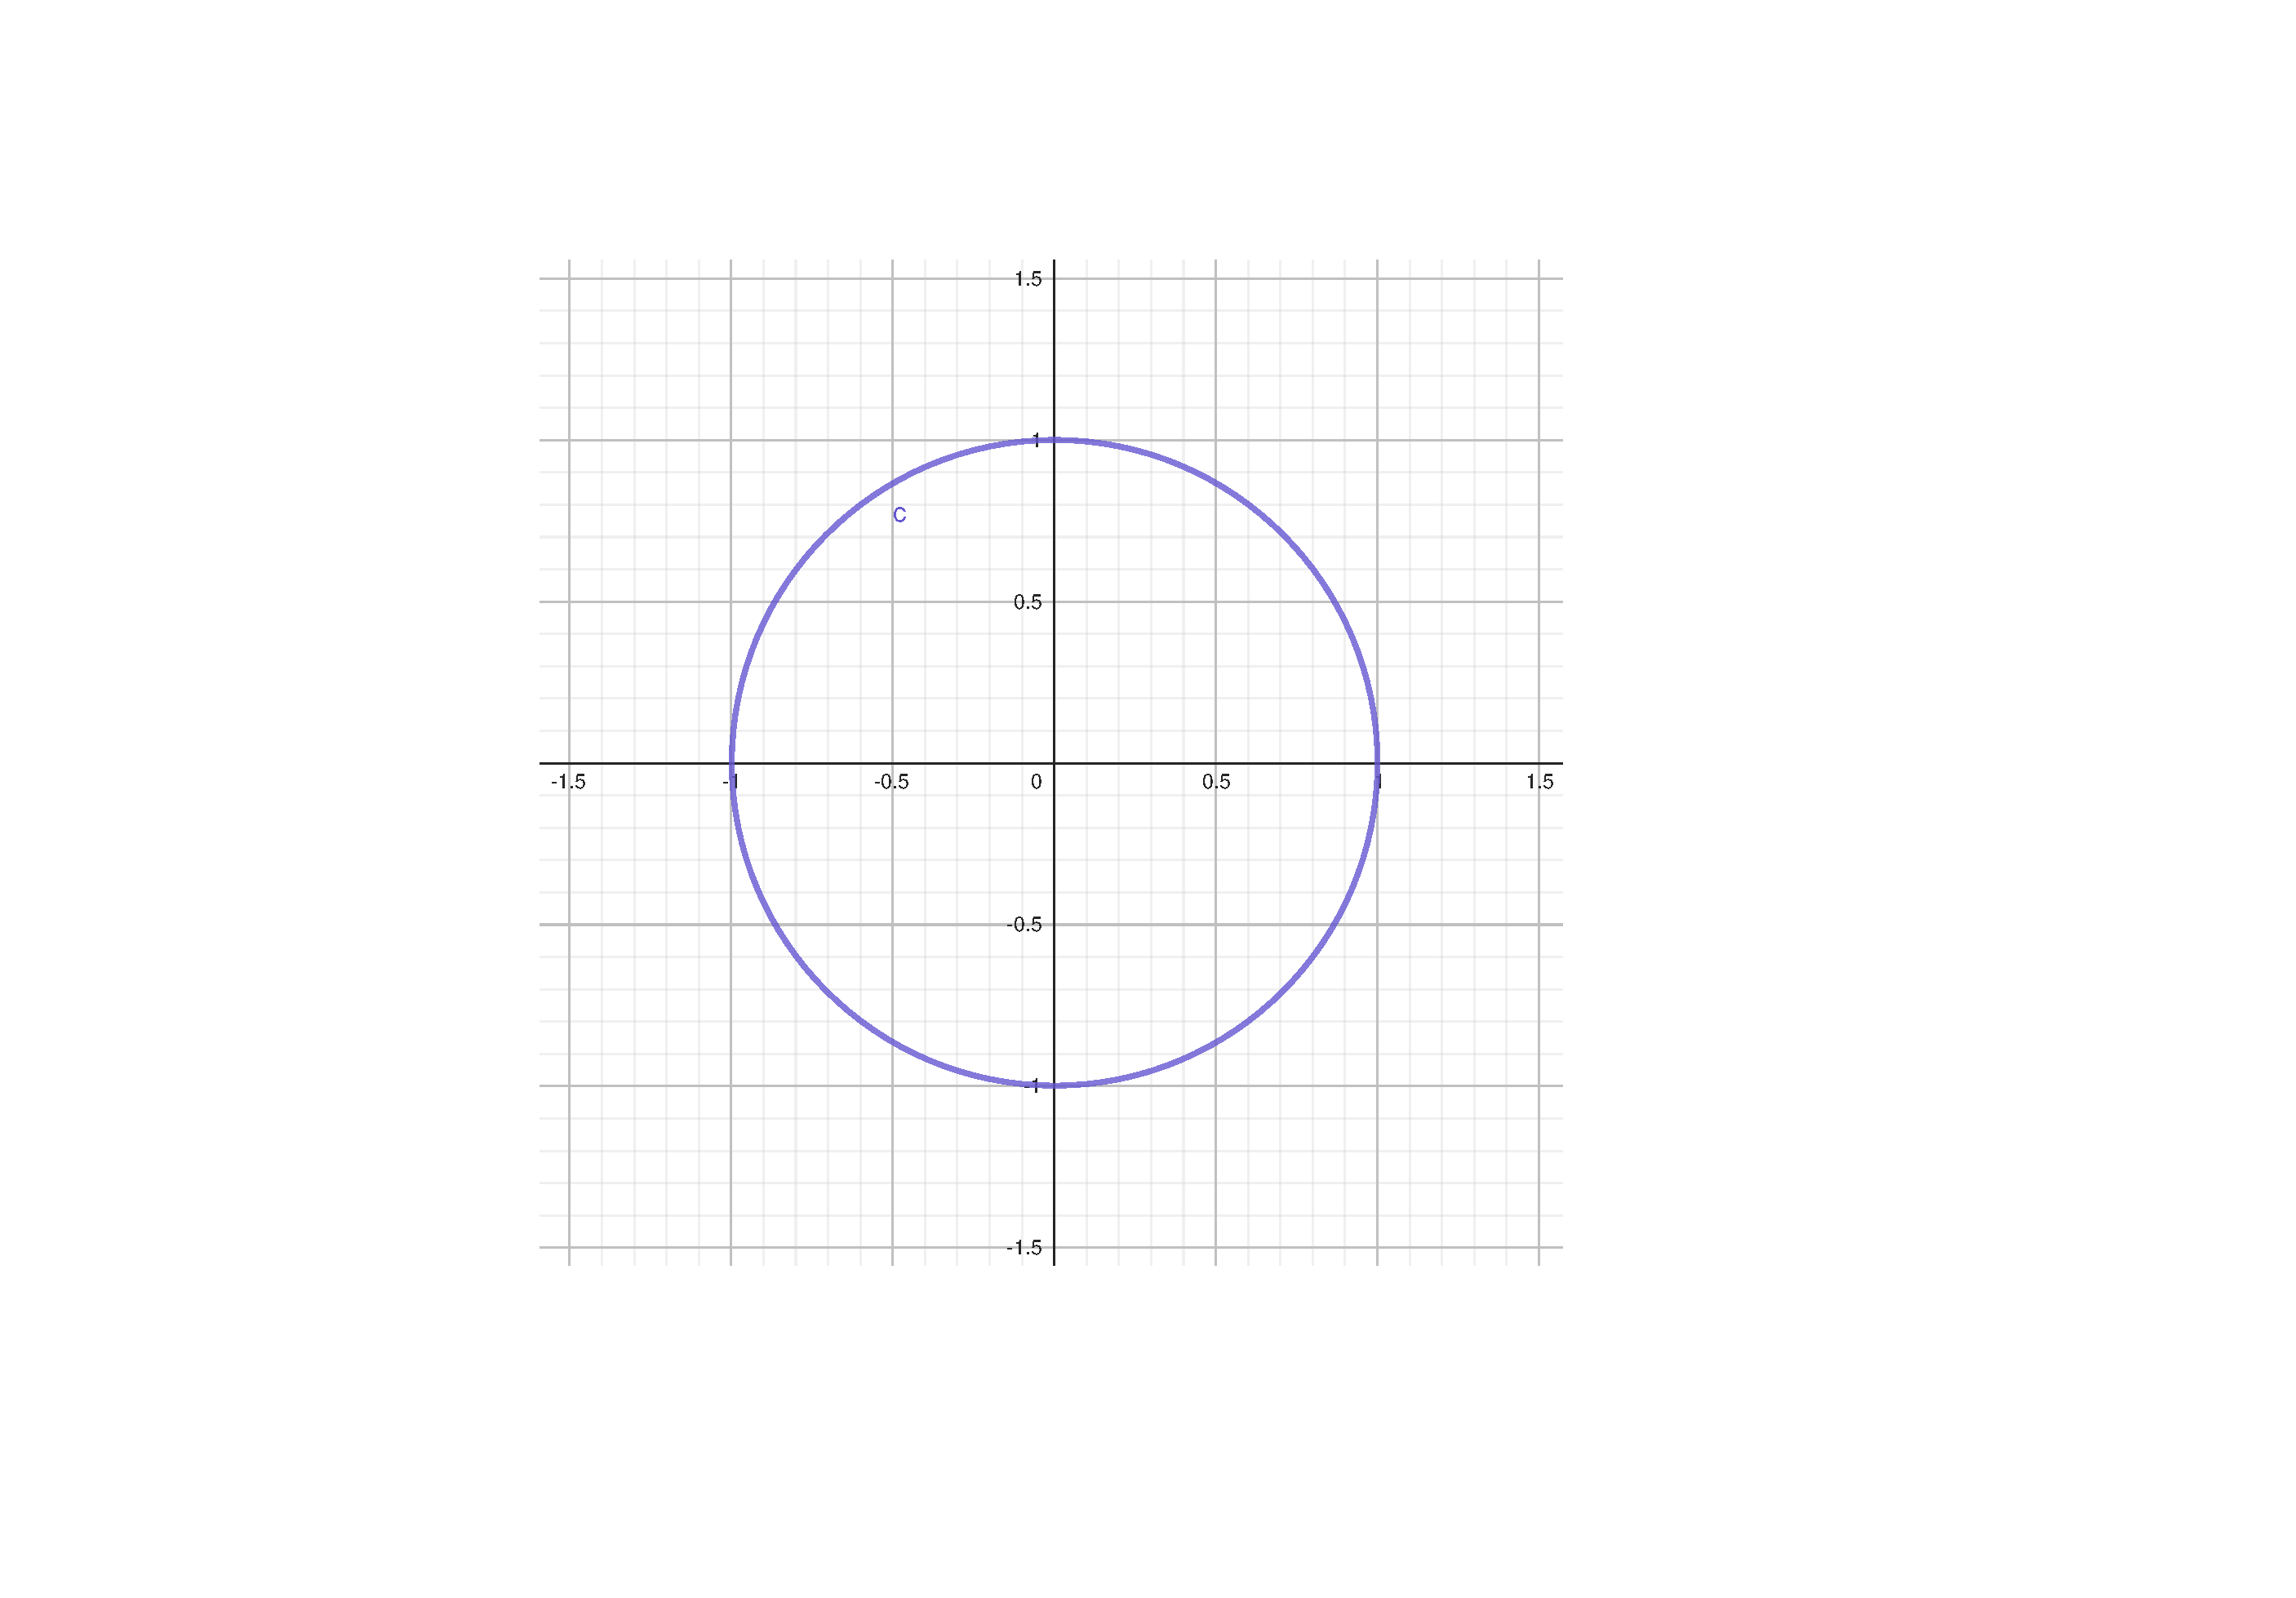
\includegraphics[width=.6\textwidth]{img/circonferenza.pdf}
	\end{figure}
	
	\noindent
	Chiamando con $C = \left(x_{C}, y_{C}\right)$ le coordinate del centro della circonferenza e con $r$ il raggio, la sua equazione generale è espressa nel seguente modo:
	\begin{equation*}
		\left(x-x_{C}\right)^{2} + \left(y-y_{C}\right)^{2} = r^{2}
	\end{equation*}
	Nel caso in cui la circonferenza fosse centrata nell'origine degli assi, ovvero $C = \left(0,0\right)$, allora l'equazione generale sarebbe ridotta a:
	\begin{equation*}
		x^{2} + y^{2} = r^{2}
	\end{equation*}
	Per essere più precisi, l'\textbf{equazione canonica} corrispondente alla circonferenza è la seguente:
	\begin{equation*}
		x^{2} + y^{2} + \alpha x + \beta y + \gamma = 0
	\end{equation*}
	Le formule più importanti per ricavare il centro della circonferenza $C$ e il raggio $r$:
	\begin{equation*}
		C = \left(-\dfrac{\alpha}{2}, -\dfrac{\beta}{2}\right) \hspace{1em} ; \hspace{1em} r = \sqrt{\dfrac{\alpha^{2}}{4} + \dfrac{\beta^{2}}{4} - \gamma}
	\end{equation*}
	Per ottenere l'equazione generale partendo dall'equazione canonica, si utilizza il metodo dei completamento dei quadrati (paragrafo~\ref{subsubsection: completamento dei quadrati}).\newline
	
	\noindent
	Per ottenere il raggio nel caso in cui sia noto il centro $C$ e un punto $P = \left(x_{P}, y_{P}\right)$ appartenente alla circonferenza, si utilizza la seguente formula:
	\begin{equation*}
		r = \sqrt{\left(x_{P} - x_{C}\right)^{2} + \left(y_{P} - y_{C}\right)^{2}}
	\end{equation*}
	Per altri approfondimenti: \href{https://www.youmath.it/formulari/formulari-di-geometria-analitica/440-circonferenza-e-cerchio-nel-piano-cartesiano.html}{YouMath}.\newpage
	
	%%%%%%%%%%%
	% Ellisse %
	%%%%%%%%%%%
	\subsubsection{Ellisse}\label{subsubsection: ellisse}
	
	Non esiste un'unica rappresentazione dell'ellisse, ma solitamente può essere facilmente riconoscibile perché di forma allungata:
	\begin{figure}[!htp]
		\centering
		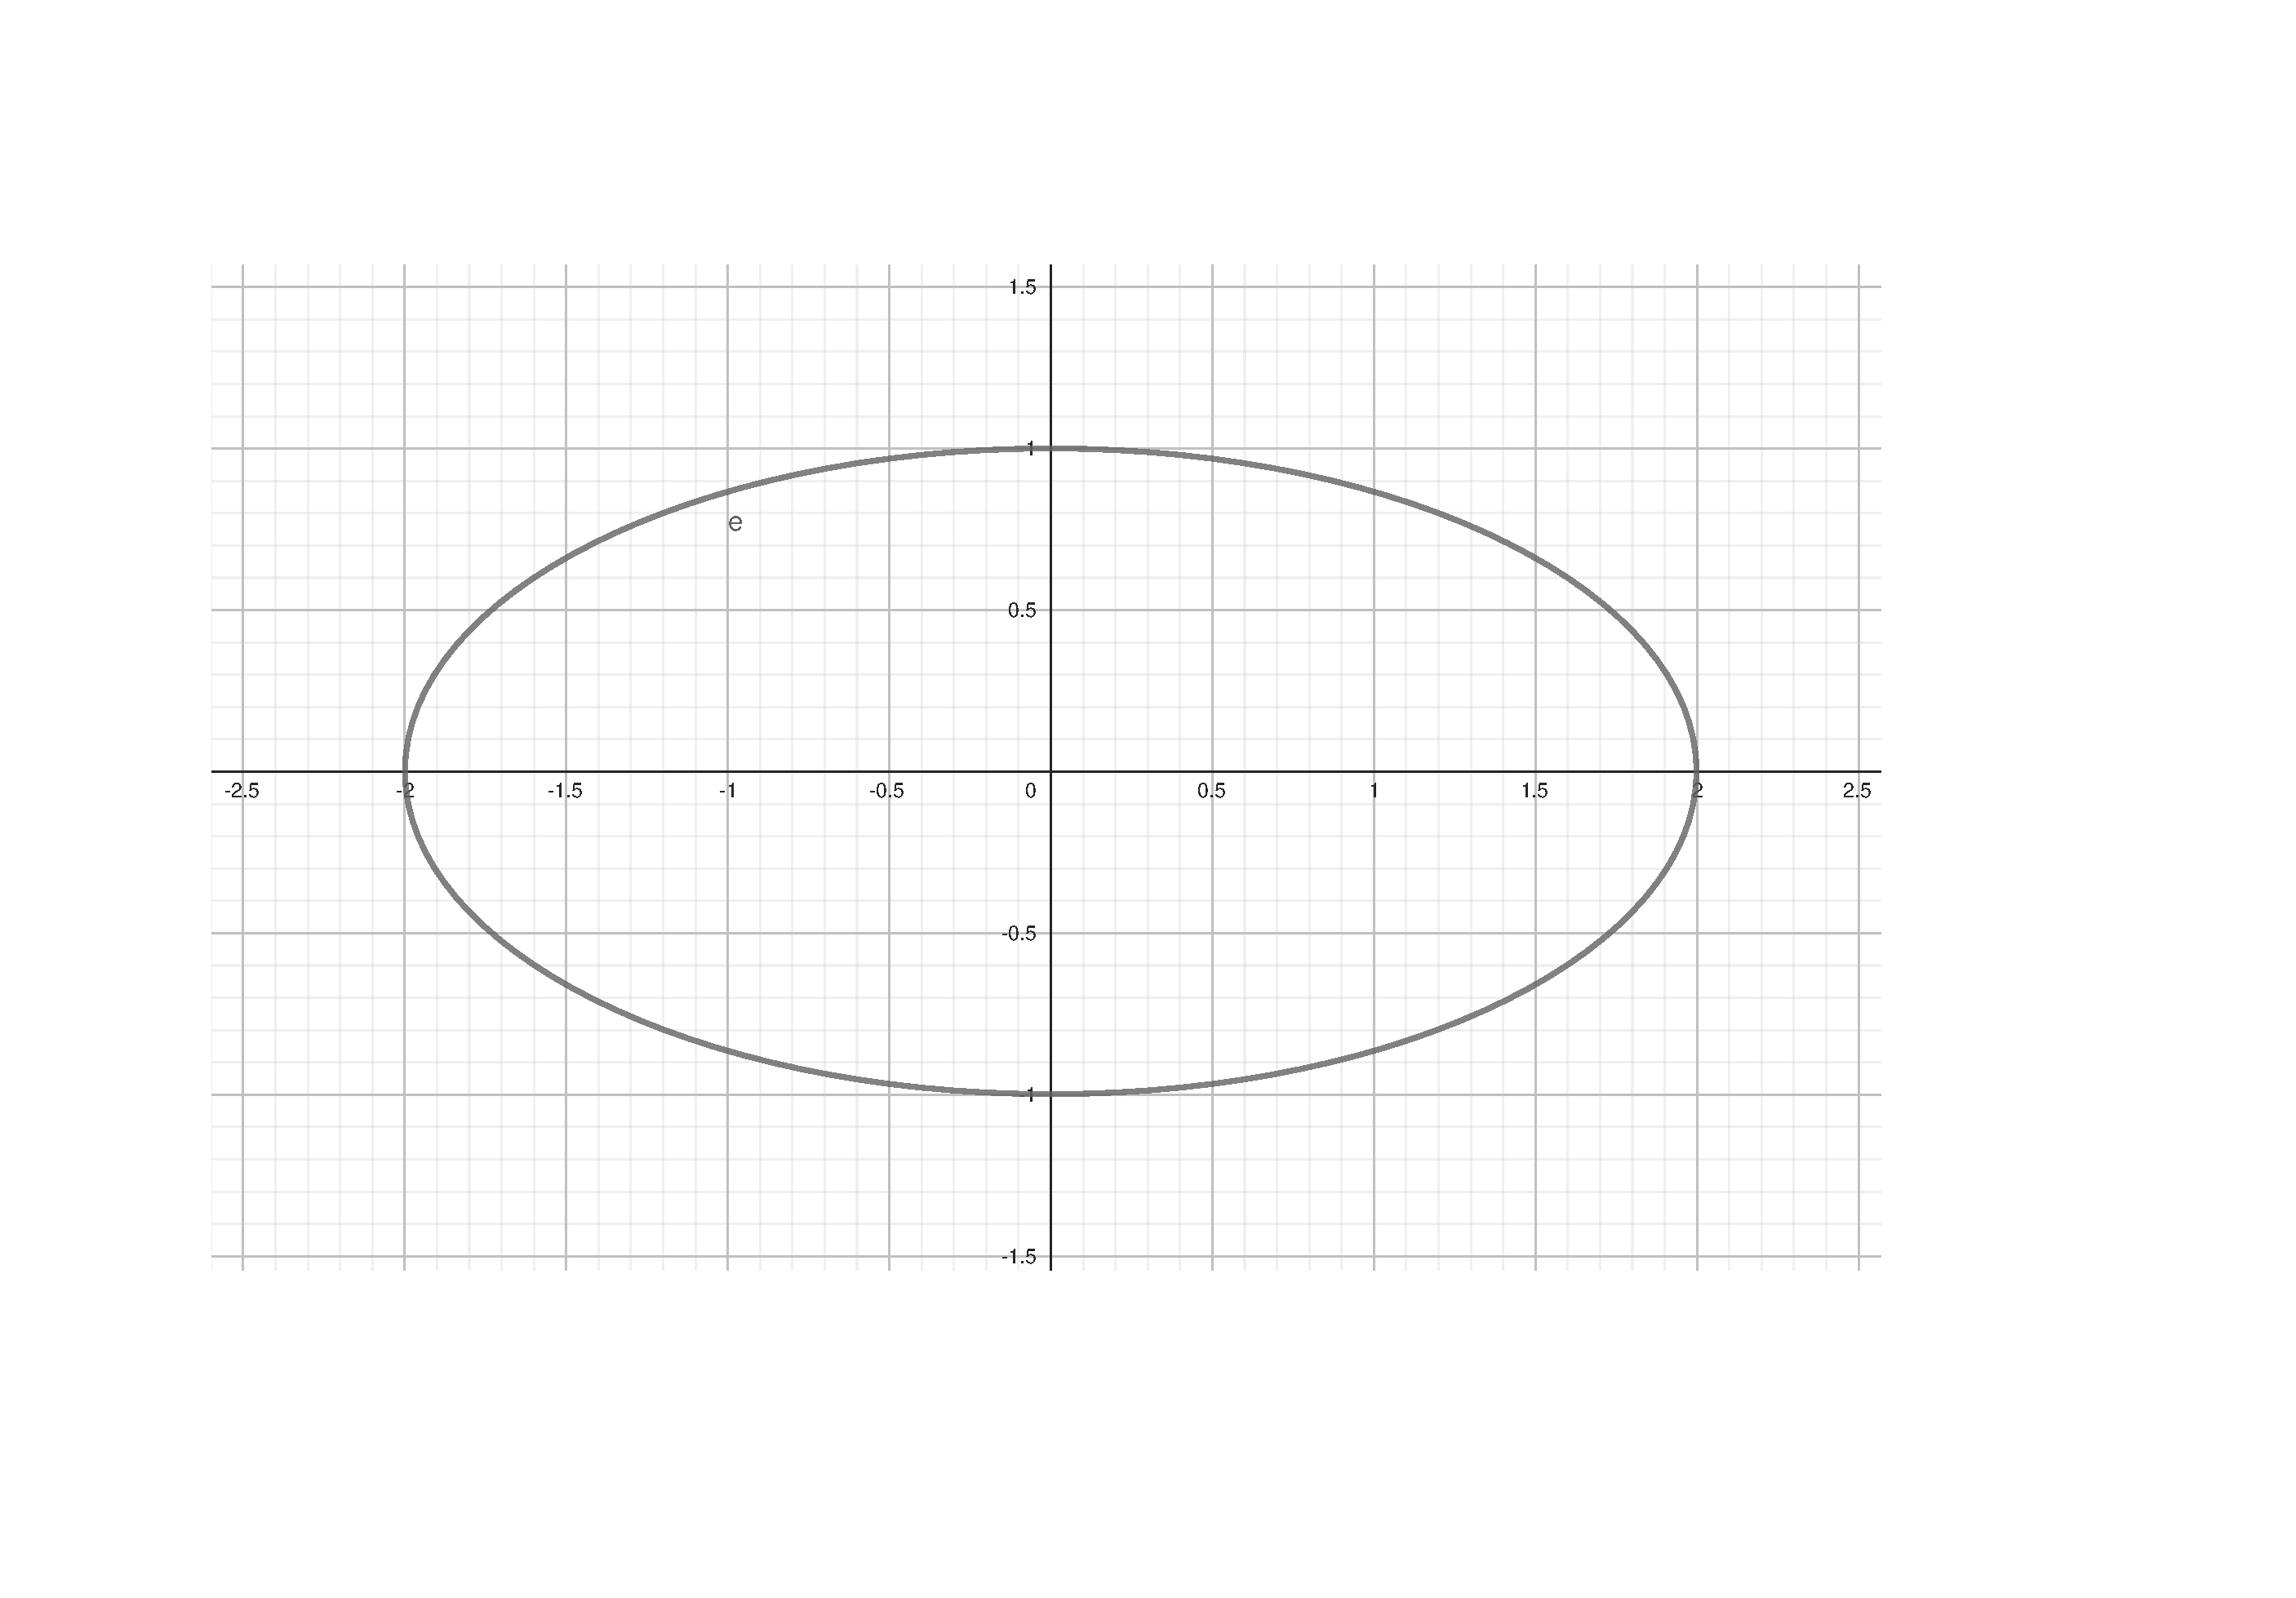
\includegraphics[width=.6\textwidth]{img/ellisse.pdf}
	\end{figure}
	
	\noindent
	Attenzione, che data l'\textbf{equazione canonica} dell'ellisse \textbf{centrata nell'origine}:
	\begin{equation*}
		\dfrac{x^{2}}{a^{2}} + \dfrac{y^{2}}{b^{2}} = 1 \hspace{2em} a \ne 0, \:\: b \ne 0
	\end{equation*}
	Il grafico corrisponde esattamente ad una circonferenza.\newline
	
	\noindent
	Un'ellisse presenta quattro vertici nel caso in cui abbia centro nell'origine. Le relative coordinate sono:
	\begin{equation*}
		V_{1,2} = \left(\pm a, 0\right) \hspace{1em} V_{3,4} = \left(0, \pm b\right)
	\end{equation*}
	Per calcolare l'eccentricità di un'ellisse (\dquotes{quanto l'ellisse è schiacciata}) si devono confrontare i due valori $a^{2}$ e $b^{2}$:
	\begin{equation*}
		\begin{array}{rclcl}
			e = \dfrac{c}{a} & \text{se} & a^{2} > b^{2} & \text{e quindi} & c = \sqrt{a^{2} - b^{2}}\\ [1em]
			e = \dfrac{c}{b} & \text{se} & b^{2} > a^{2} & \text{e quindi} & c = \sqrt{b^{2} - a^{2}}
		\end{array}
	\end{equation*}
	Il valore è compreso tra: $0 \le e < 1$.\newline
	
	\noindent
	Nel caso in cui non fosse centrata nell'origine, l'\textbf{equazione canonica} di un'\textbf{ellisse traslata}, con $C=\left(x_{C}, y_{C}\right)$ come coordinate del centro:
	\begin{equation*}
		\dfrac{\left(x-x_{C}\right)^{2}}{a^{2}} + \dfrac{\left(y-y_{C}\right)^{2}}{b^{2}} = 1
	\end{equation*}
	I relativi vertici hanno le seguenti coordinate:
	\begin{equation*}
		\begin{array}{lcl}
			V_{1} = \left(x_{C}-a, y_{C}\right) &;& V_{2} = \left(x_{C}+a, y_{C}\right) \\
			V_{3} = \left(x_{C}, y_{C}-b\right) &;& V_{4} = \left(x_{C}, y_{C}+b\right) \\
		\end{array}
	\end{equation*}
	L'\textbf{importanza dei vertici} è dovuta al fatto che se fosse necessario rappresentare l'ellisse su un piano cartesiano, grazie alle precedenti formule. È possibile ricordarsi facilmente le formule ricordando che le coordinate dei vertici sono ottenute eseguendo la somma/differenza prima sulla coordinata $x$ e poi sulla coordinata $y$.\newline
	
	\noindent
	Per altri approfondimenti: \href{https://www.youmath.it/formulari/formulari-di-geometria-analitica/445-ellisse-nel-piano-cartesiano.html}{YouMath}.\newpage

	%%%%%%%%%%%%
	% Iperbole %
	%%%%%%%%%%%%
	\subsubsection{Iperbole}\label{subsubsection: iperbole}

	Un iperbole con centro nell'origine ha un'equazione del tipo:
	\begin{equation*}
		\dfrac{x^{2}}{a^{2}} - \dfrac{y^{2}}{b^{2}} = \pm 1 \hspace{1.5em} \text{con } a \ne 0, \: b \ne 0
	\end{equation*}
	Il segno $+$ accanto all'$1$ rappresenta l'intersezione con l'asse delle ascisse ($x$), mentre il segno $-$ rappresenta l'intersezione con l'asse delle ordinate ($y$). Graficamente viene rappresentata nel seguente modo:\newline

	\begin{minipage}{.6\textwidth}
		\centering
		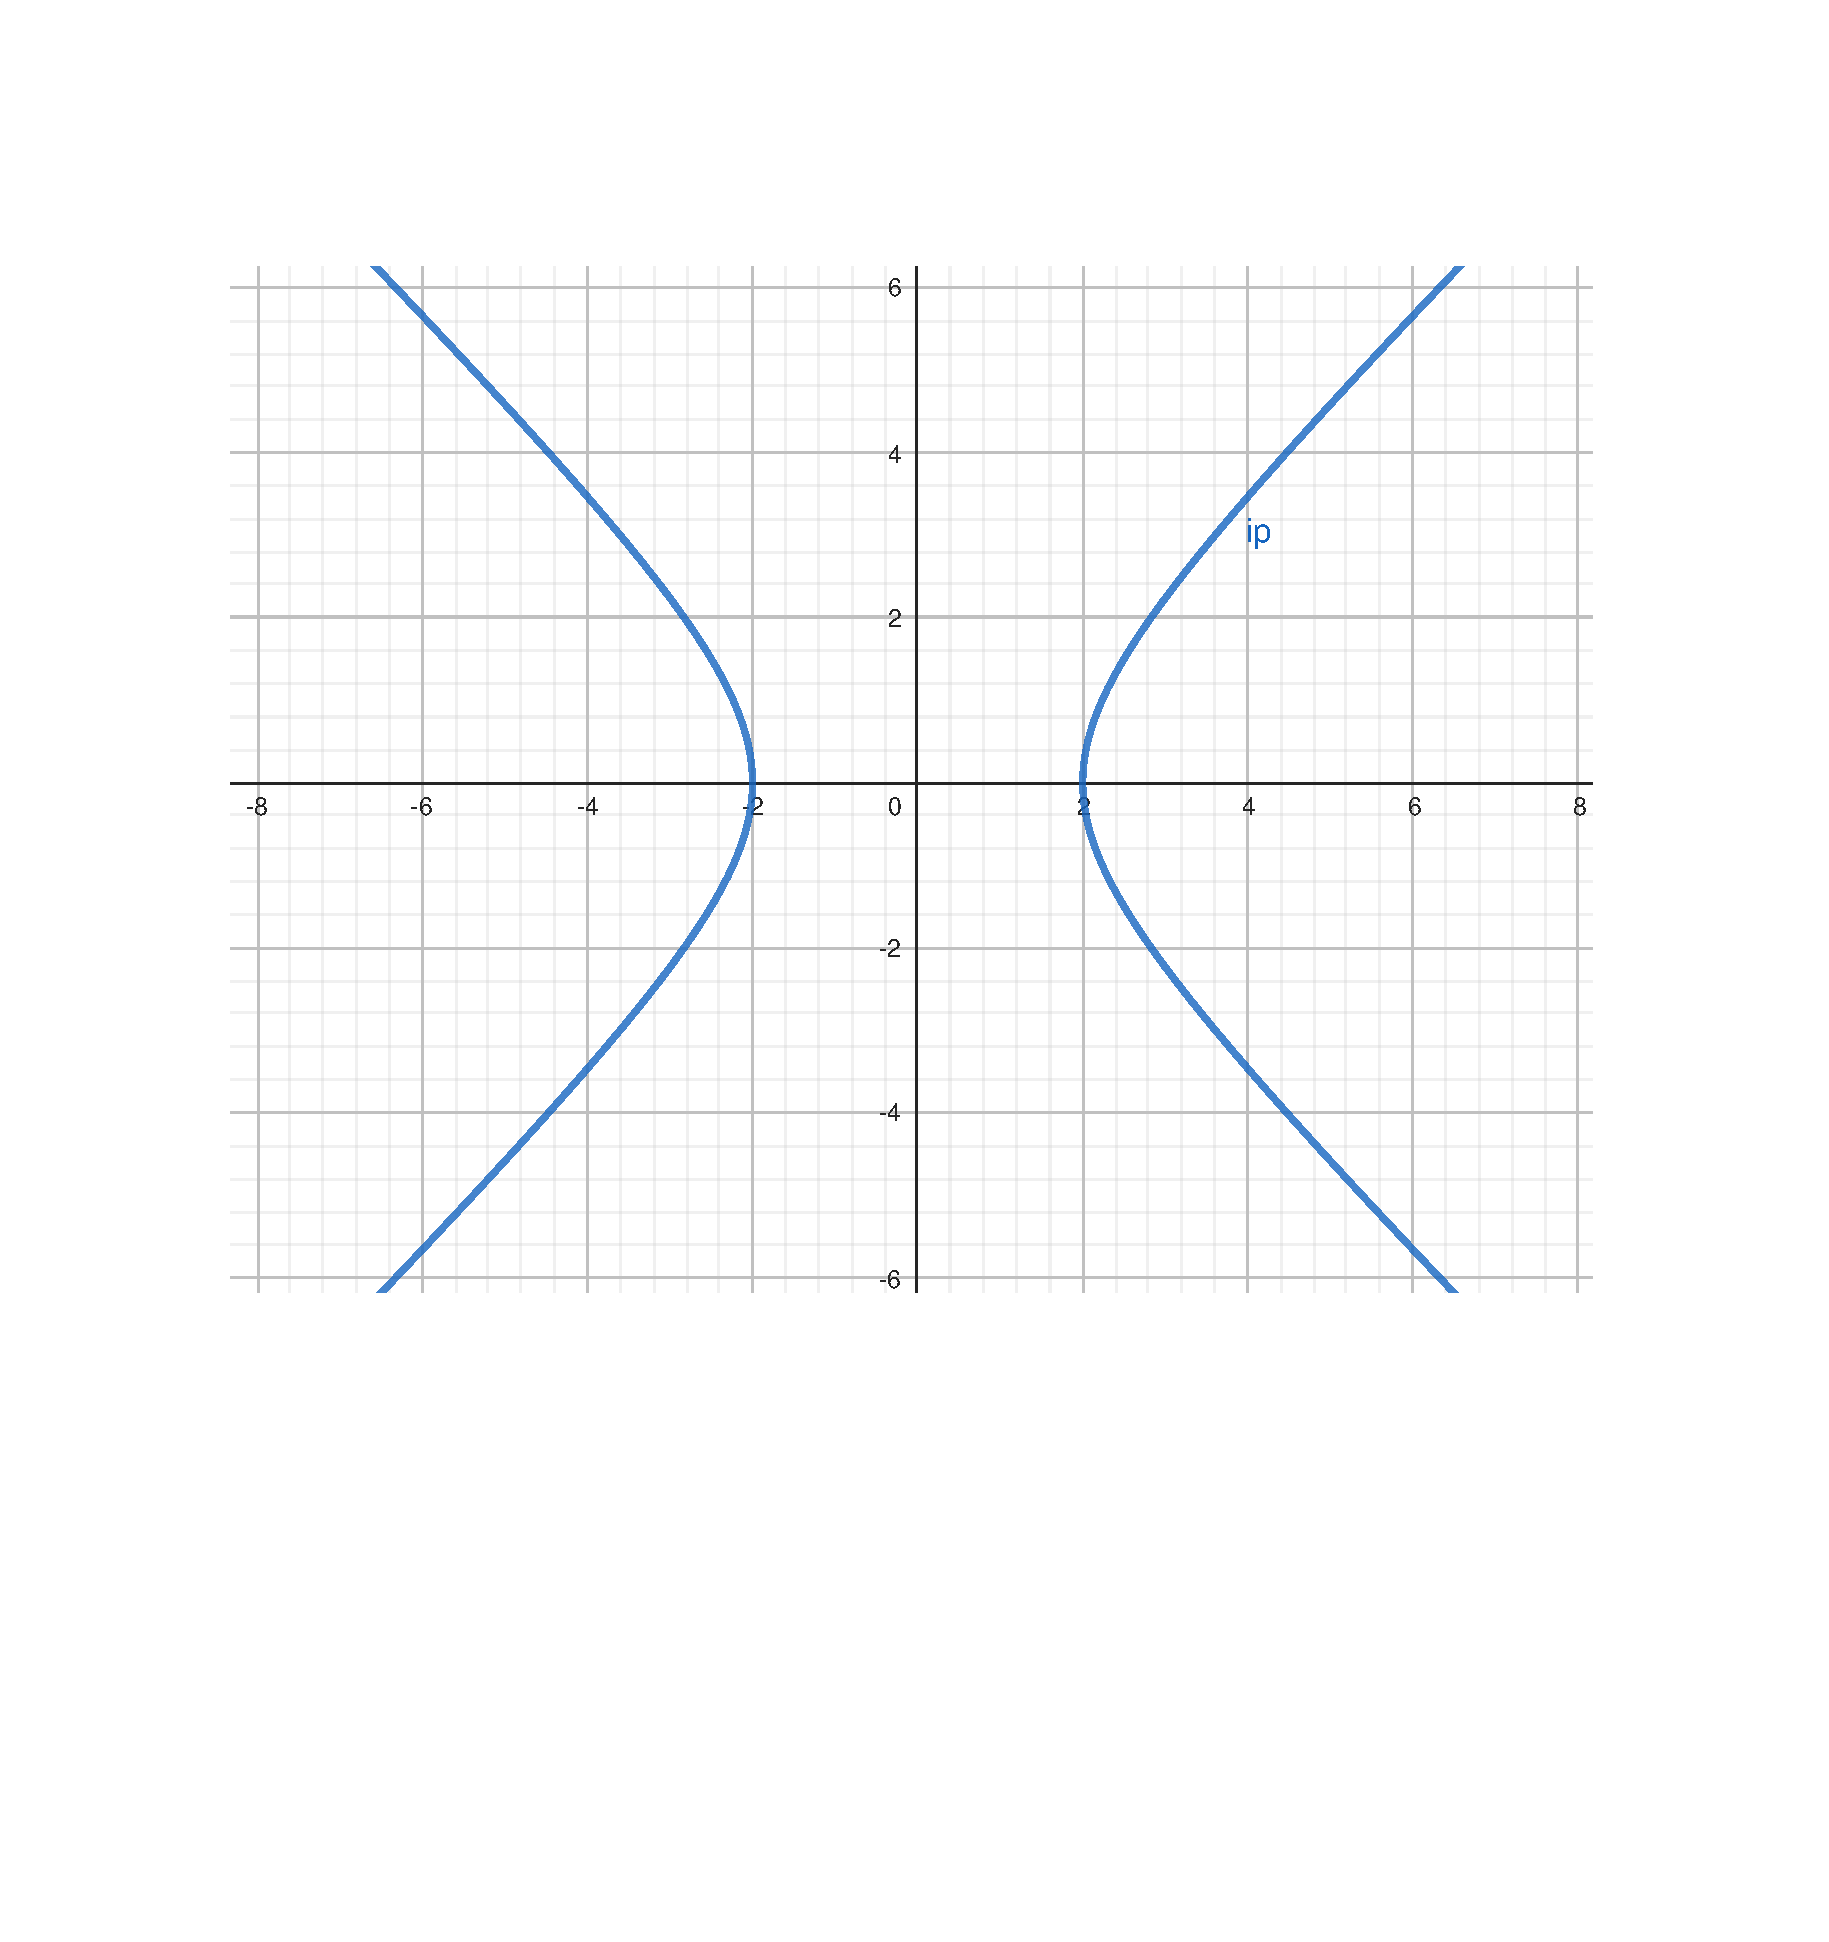
\includegraphics[width=\textwidth]{img/iperbole_ascisse.pdf}
		
		\noindent
		Con $+1$.
	\end{minipage}
	\begin{minipage}{.4\textwidth}
		\centering
		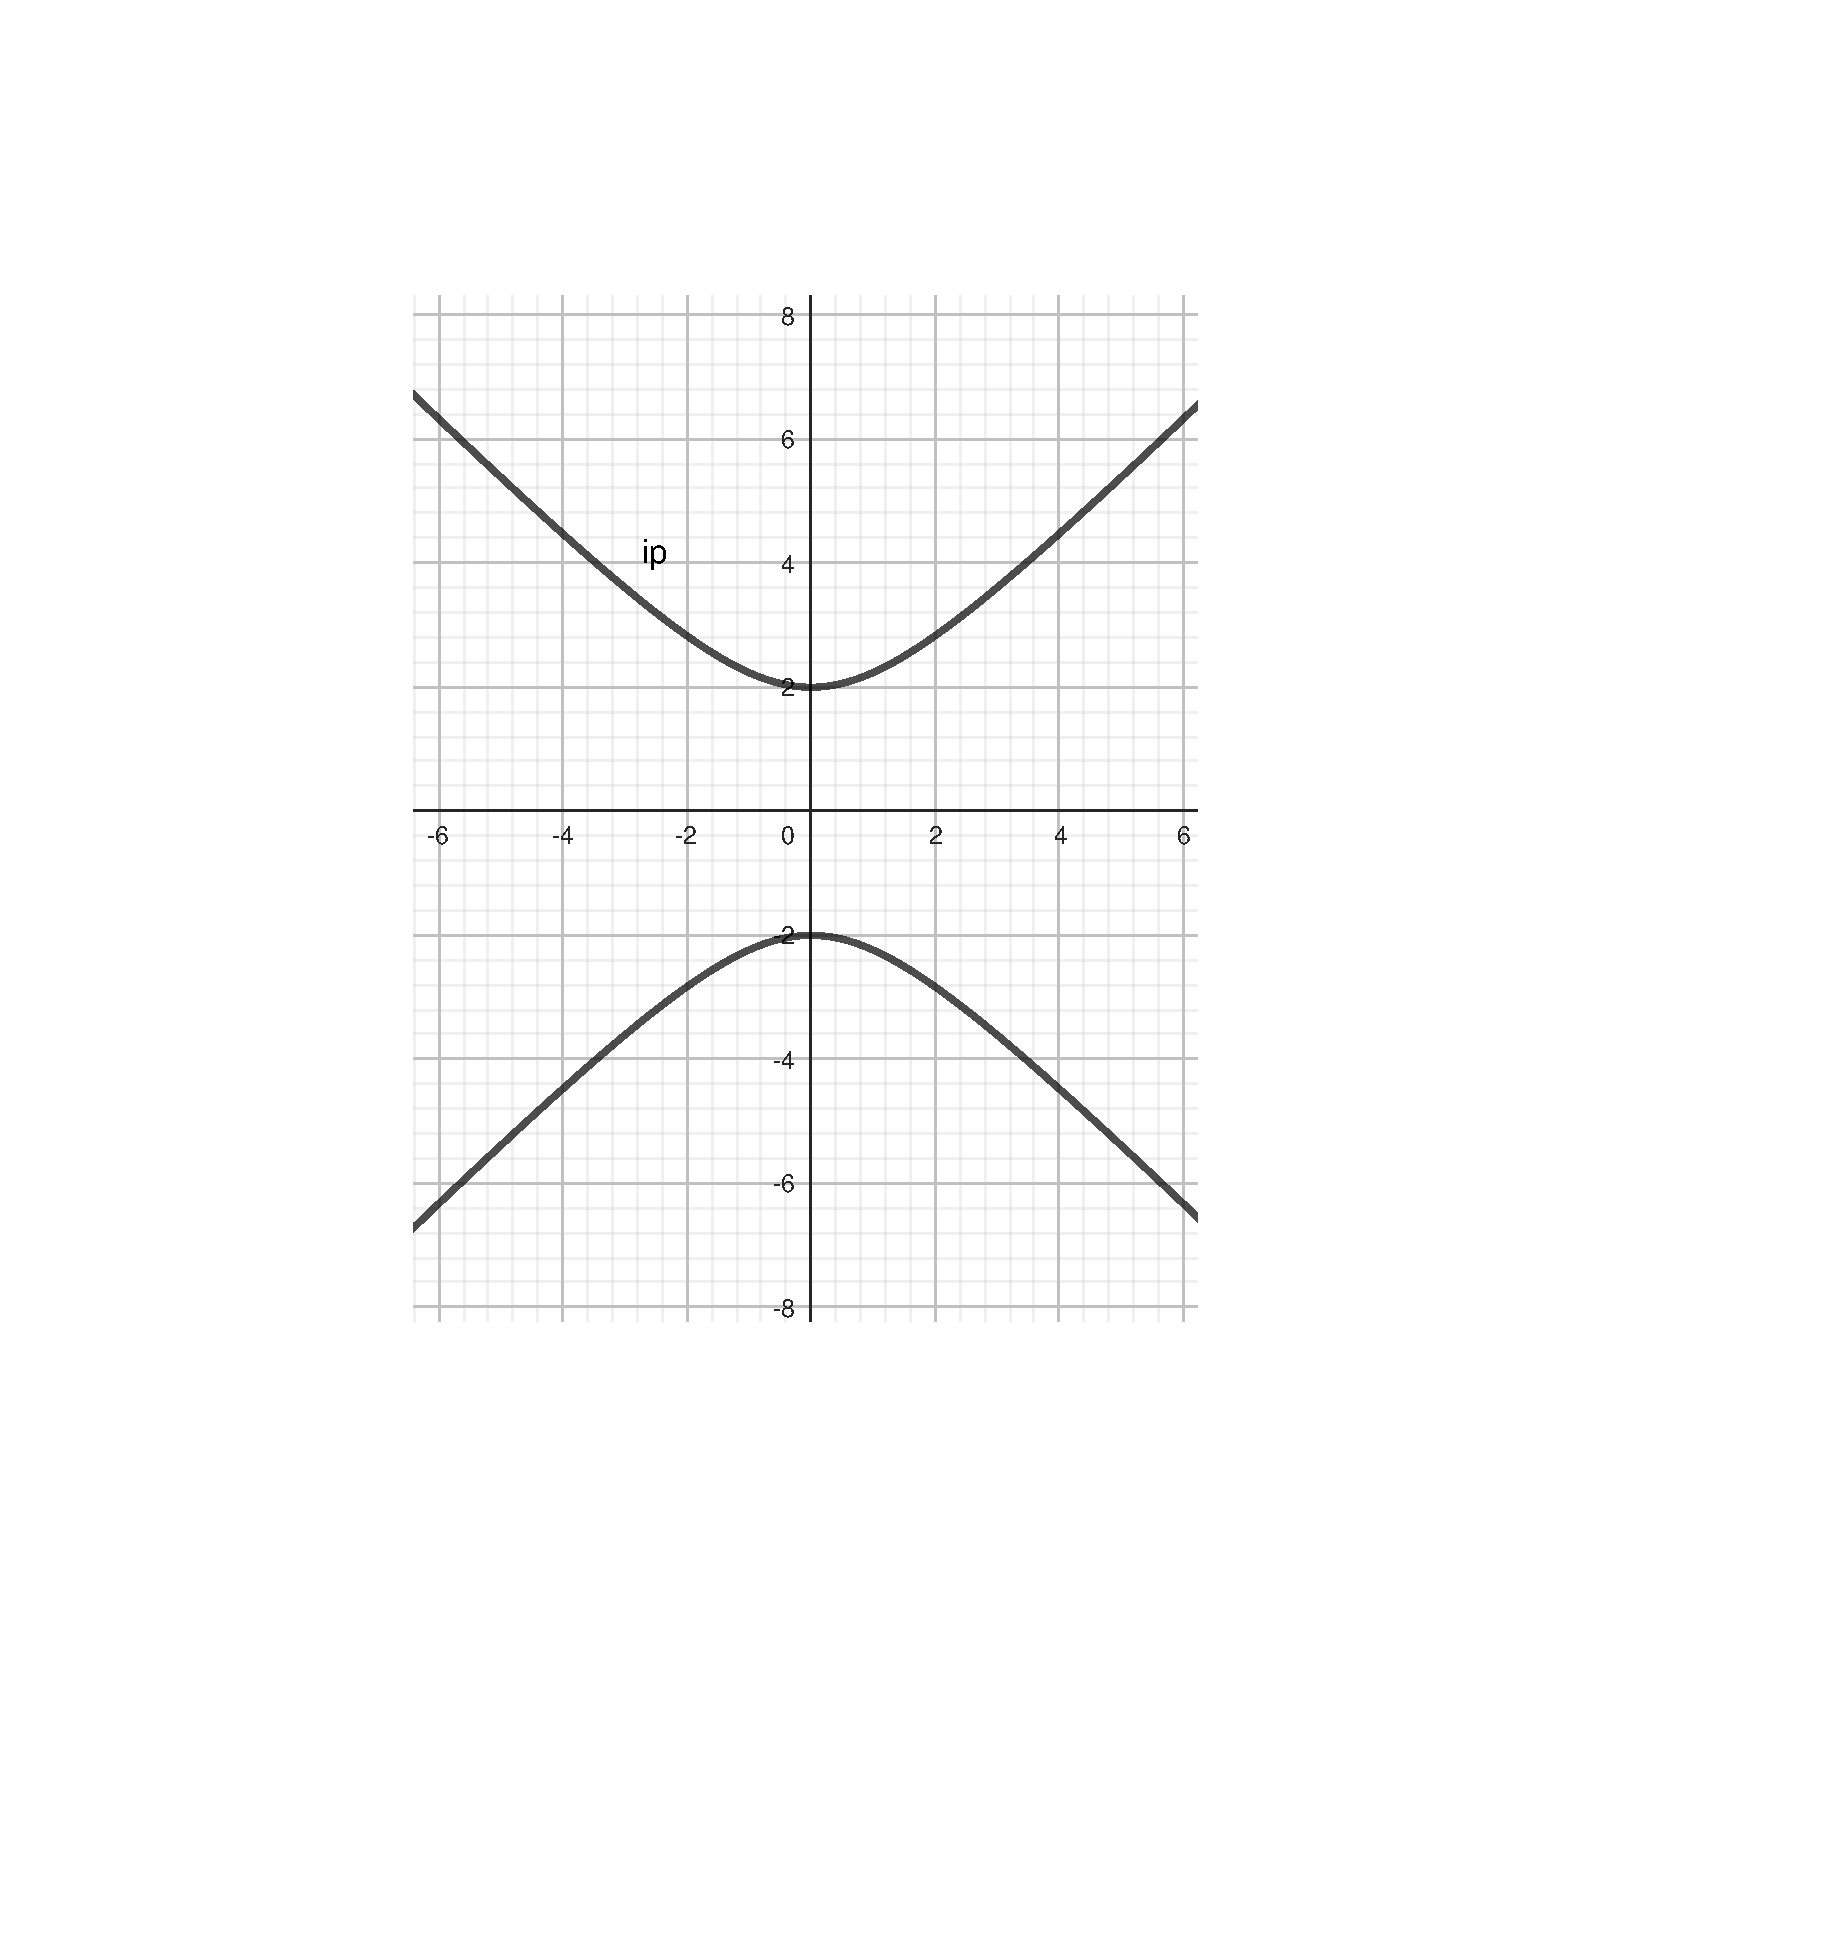
\includegraphics[width=.9\textwidth]{img/iperbole_ordinate.pdf}
		
		\noindent
		Con $-1$.
	\end{minipage}\newline

	\noindent
	Nel caso di una iperbole con gli assi paralleli agli assi cartesiani e quindi con centro in un punto $C = \left(x_{C}, y_{C}\right)$, essa è data da:
	\begin{equation*}
		\dfrac{\left(x-x_{C}\right)^{2}}{a^{2}} - \dfrac{\left(y-y_{C}\right)^{2}}{b^{2}} = \pm 1 \hspace{1.5em} \text{con } a \ne 0, \: b \ne 0
	\end{equation*}
	Dove il segno $\pm$ accanto all'$1$ indica la stessa cosa detta in precedenza.\newline
	
	\noindent
	Il calcolo dei vertici, utile per rappresentare l'iperbole, ricorda molto quello utilizzato per l'ellisse. Tuttavia, dato che in questo caso i vertici sono solo 2 e non 4 (ellisse), tale calcolo cambia a seconda dell'intersezione con l'asse delle $x$ o delle $y$ (determinato dal segno $\pm$ dell'$1$ a sinistra dell'uguale):
	\begin{equation*}
		\begin{array}{rcl}
			\text{Intersezione asse }x\text{, caso }+1 &\rightarrow& V_{1} = \left(x_{C}-a, y_{C}\right) \\ [.3em]
			&& V_{2} = \left(x_{C}+a, y_{C}\right) \\ [1em]
			%
			\text{Intersezione asse }y\text{, caso }-1 &\rightarrow& V_{1} = \left(x_{C}, y_{C}-b\right) \\ [.3em]
			&& V_{2} = \left(x_{C}, y_{C}+b\right)
		\end{array}
	\end{equation*}
	Purtroppo tutto questo non basta per rappresentare un'iperbole, è necessario calcolare anche gli asintoti di un'iperbole per capire l'andamento dell'iperbole. Gli asintoti sono due punti dai quali passa una retta, la quale non viene mai toccata dall'iperbole:
	\begin{equation*}
		\begin{array}{rcl}
			\text{Intersezione asse }x\text{, caso }+1 &\rightarrow& \text{asintoto } = \left(V_{x}, \pm\dfrac{b}{a} + V_{y}\right) \\ [1em]
			%
			\text{Intersezione asse }y\text{, caso }-1 &\rightarrow& \text{asintoto } = \left(\pm\dfrac{b}{a} + V_{x}, V_{y}\right)
		\end{array}
	\end{equation*}
	Con $V_{x},V_{y}$ si intendono le coordinate $x,y$ dei vertici.\newline

	\noindent
	Ricapitolando, i passi per disegnare un'iperbole partendo dall'equazione canonica sono:
	\begin{enumerate}
		\item Posizionarsi sulle coordinate di centro $x_{C}, y_{C}$

		\item Calcolare i vertici, aumentando/diminuendo la $x_{C}$ se l'$1$ nell'equazione canonica ha segno $+$, altrimenti aumentando/diminuendo la $y_{C}$ se l'$1$ nell'equazione canonica ha segno $-$
		
		\item Individuare i punti del fuoco e far passare una retta, per ciascun punto, passante per il centro $x_{C}, y_{C}$
		
		\item Disegnare l'iperbole evitando di toccare le assi
	\end{enumerate}
	Un esempio si può vedere nel seguente grafico:
	\begin{figure}[!htp]
		\centering
		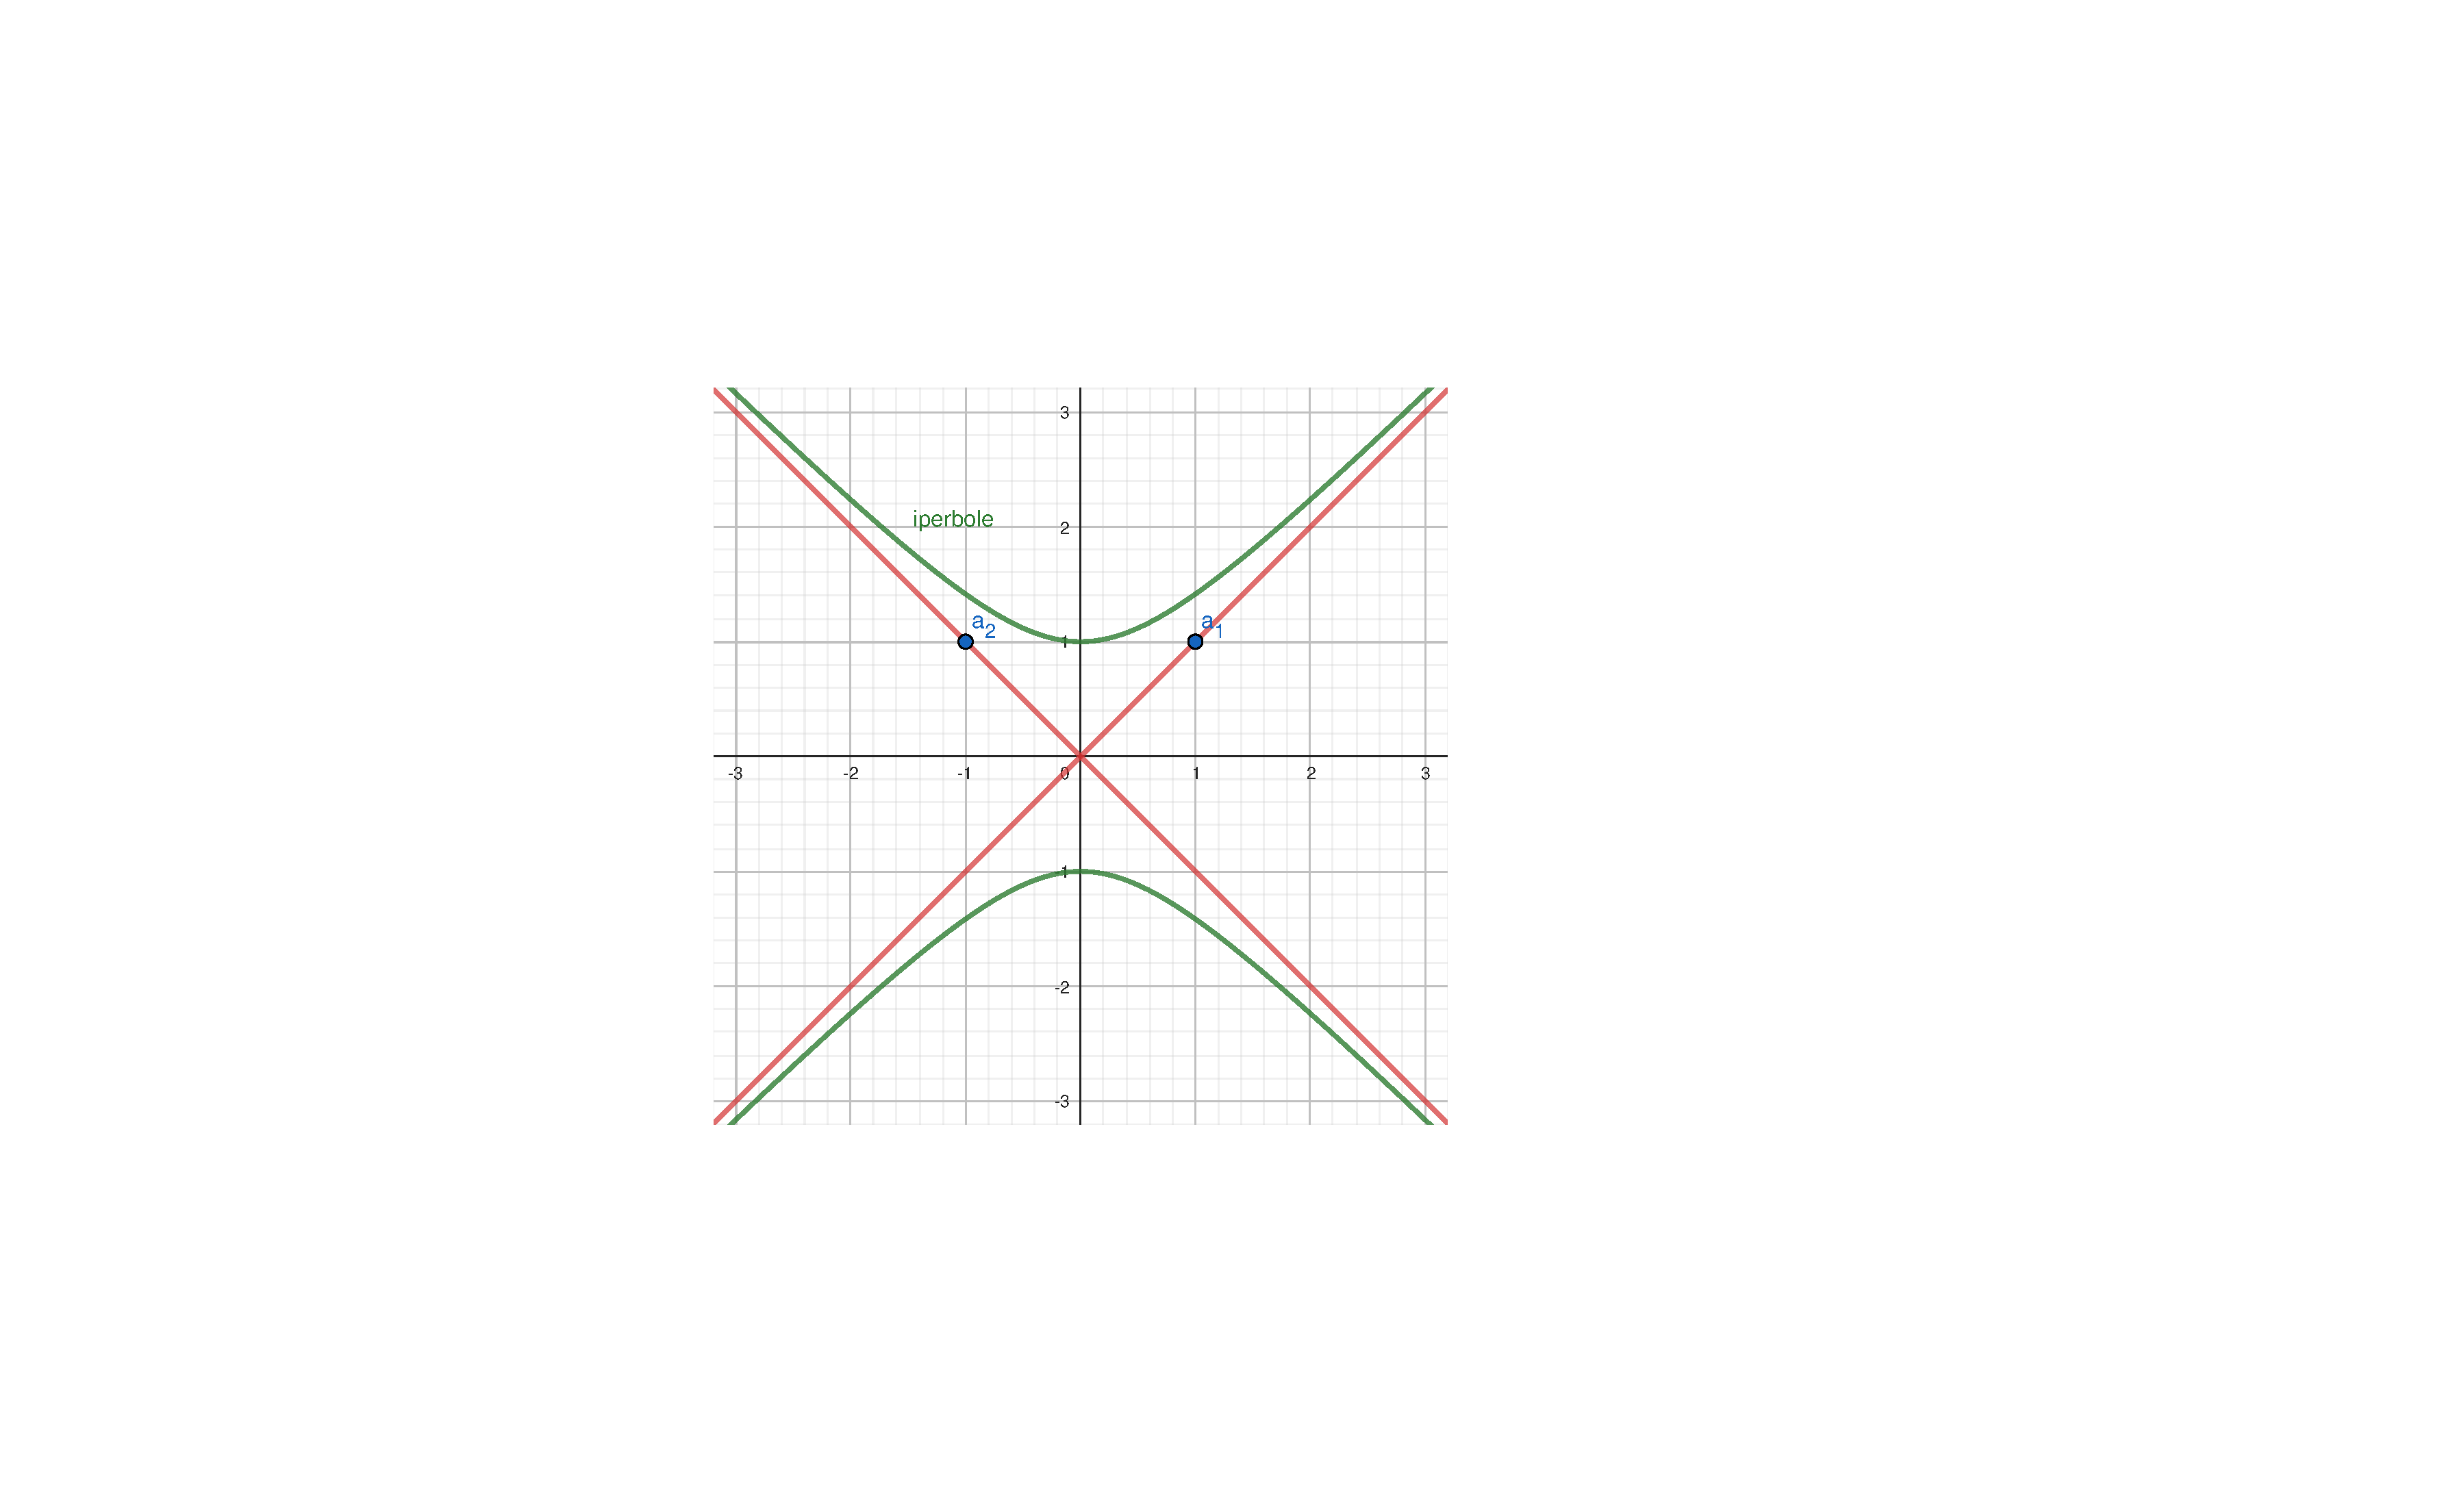
\includegraphics[width=.7\textwidth]{img/iperbole_esempio.pdf}
		\caption*{Iperbole di equazione: $x^{2} - y^{2} = -1$}
	\end{figure}

	\noindent
	Ovviamente le rette non vanno disegnate, ma in questo grafico sono state rappresentate per mostrare come disegnare un'iperbole.

	\noindent
	Per altri approfondimenti: \href{https://www.youmath.it/formulari/formulari-di-geometria-analitica/453-iperbole-nel-piano-cartesiano.html}{YouMath}.\newpage
	
	%%%%%%%%%%%%%%%%%%%%%%%%%%%%%%
	% Completamento dei quadrati %
	%%%%%%%%%%%%%%%%%%%%%%%%%%%%%%
	\subsubsection{Completamento dei quadrati}\label{subsubsection: completamento dei quadrati}
	
	Il completamento dei quadrati è un'operazione molto potente che può essere applicata sempre (a discapito dello studente se ha senso o no applicarla!). In questo caso viene applicata ad un'ellisse.\newline
	
	\noindent
	Innanzitutto, la \textbf{prima operazione} dell'applicazione del completamento dei quadrati è il raggruppamento dei valori simili, ovverosia:
	\begin{equation*}
		\begin{array}{rcl}
			9x^{2} + 4y^{2} + 36x - 24y + 36 &=& 0 \\
			\left(9x^{2} + 36x\right) + \left(4y^{2} - 24y\right) + 36 &=& 0
		\end{array}
	\end{equation*}
	La \textbf{seconda operazione} è prendere in considerazione i termini con le $x$, e poi quelli con le $y$, e cercare un quadrato. Ovvero sia un valore $c$ tale per cui il $\Delta$ (nella formula del calcolo di un'equazione di secondo grado $\Delta = b^{2} - 4 \cdot a \cdot c$) sia uguale a zero:
	\begin{equation*}
		\begin{array}{rcl}
			9x^{2} + 36x &\longrightarrow& 36^{2} - 4 \cdot 9 \cdot c = 0 \\
			&& 36^{2} - 36c = 0 \\
			&& c = 36 \\ [1em]
			4y^{2} - 24y &\longrightarrow& 24^{2} - 4 \cdot 4 \cdot c = 0 \\
			&& 24^{2} - 16c = 0 \\
			&& c = 36
		\end{array}
	\end{equation*}
	\underline{Suggerimento}: per trovare tale valore, basta risolvere la banale equazione $b^{2} - 4 \cdot a \cdot c = 0$ con $c$ incognita e $a,b$ termini noti.\newline
	
	\noindent
	La \textbf{terza operazione} è riscrivere l'equazione con i nuovi valori $c$, ma per lasciare invariata l'equazione è necessario annullarli, ovvero scrivere $c-c$ (nessun problema, con manipolazioni algebriche si riuscirà ad evitare di ritornare al punto di inizio):
	\begin{equation*}
		\left(9x^{2} + 36x + 36 - 36\right) + \left(4y^{2} - 24y + 36 - 36\right) + 36 = 0
	\end{equation*}
	Le manipolazioni algebriche riguardano $9x^{2} + 36x + 36$ e $4y^{2} - 24y + 36$. Ovvero, si riscrivono le due espressioni come quadrati!
	\begin{equation*}
		\begin{array}{rcl}
			9x^{2} + 36x + 36 &\longrightarrow& 9\left(x+2\right)^{2} \\
			4y^{2} - 24y + 36 &\longrightarrow& 4\left(y-3\right)^{2} \\
		\end{array}
	\end{equation*}
	E si riscrive l'equazione generale:
	\begin{equation*}
		9\left(x+2\right)^{2} - 36 + 4\left(y-3\right)^{2} - 36 + 36 = 0
	\end{equation*}
	Banali semplificazioni algebriche:
	\begin{equation*}
		\begin{array}{rcl}
			9\left(x+2\right)^{2} \cancel{- 36} + 4\left(y-3\right)^{2} - 36 \cancel{+ 36} &=& 0 \\ [1em]
			\dfrac{1}{36} \cdot \cancel{9}\left(x+2\right)^{2} + \cancel{4}\left(y-3\right)^{2} &=& \cancel{36} \cdot \dfrac{1}{\cancel{36}}  \\ [1em]
			\dfrac{\left(x+2\right)^{2}}{4} + \dfrac{\left(y-3\right)^{2}}{9} &=& 1
		\end{array}
	\end{equation*}
	Quest'ultima equazione corrisponde all'equazione canonica dell'ellisse.\newpage

	%%%%%%%%%%%%
	% Esercizi %
	%%%%%%%%%%%%
	\subsubsection{Esercizi}\label{subsubsection: esercizi (geometria analitica)}
	
	Si rappresenti analiticamente le seguenti equazioni canoniche:
	\begin{enumerate}
		\item $x^{2} + y^{2} - 4x + 2y - 6 = 0$
		
		\item $x^{2} + 4y^{2} - 1 = 0$
		
		\item $x^{2} - 4y^{2} - 1 = 0$
		
		\item $x^{2} - y^{2} + x + 4y - 4 = 0$
		
		\item $2x^{2} + y^{2} + 4x - y = 0$
	\end{enumerate}
	
	\begin{flushleft}
		\example{\underline{Esercizio 1}}
	\end{flushleft}
	
	\noindent
	Data l'equazione:
	\begin{equation*}
		x^{2} + y^{2} - 4x + 2y - 6 = 0
	\end{equation*}
	Prima di rappresentare analiticamente l'equazione, è necessario guardare immediatamente i termini $x^{2}$ e $y^{2}$ per vedere se si è di fronte ad una circonferenza. Infatti, ricordando l'equazione canonica della circonferenza (pagina~\pageref{subsubsection: circonferenza}):
	\begin{equation*}
		x^{2} + y^{2} + \alpha x + \beta y + \gamma = 0
	\end{equation*}
	Si può notare una grande assomiglianza. Quindi, si procede con il calcolo delle coordinate del centro della circonferenza:
	\begin{equation*}
		C = \left(-\dfrac{\alpha}{2}, -\dfrac{\beta}{2}\right) = \left(-\dfrac{\left(-4\right)}{2}, -\dfrac{2}{2}\right) = \left(2, -1\right)
	\end{equation*}
	Si procede con il calcolo del raggio:
	\begin{equation*}
		r = \sqrt{\dfrac{\alpha^{2}}{4} + \dfrac{\beta^{2}}{4} - \gamma} = \sqrt{\dfrac{\left(-4\right)^{2}}{4} + \dfrac{\left(2\right)^{2}}{4} - \left(-6\right)} = \sqrt{4 + 1 + 6} = \sqrt{11}
	\end{equation*}
	Infine, si scrive l'equazione canonica sostituendo i valori trovati:
	\begin{equation*}
		\begin{array}{rcl}
			\left(x-x_{C}\right)^{2} + \left(y-y_{C}\right)^{2} &=& r^{2} \\ [1em]
			\left(x-2\right)^{2} + \left(y+1\right)^{2} &=& 11
		\end{array}
	\end{equation*}
	
	\begin{flushleft}
		\example{\underline{Esercizio 2}}
	\end{flushleft}
	
	\noindent
	Data l'equazione:
	\begin{equation*}
		x^{2} + 4y^{2} - 1 = 0
	\end{equation*}
	Con una piccola manipolazione algebrica si può subito vedere che si è di fronte ad un'ellisse centrata nell'origine:
	\begin{equation*}
		x^{2} + 4y^{2} = 1
	\end{equation*}
	Si procede con un po' di intuito così da ricavare la forma canonica:
	\begin{equation*}
		\dfrac{\left(x-0\right)^{2}}{1^{2}} + \dfrac{\left(y-0\right)^{2}}{\left(\frac{1}{2}\right)^{2}} = 1
	\end{equation*}
	E il risultato (forma canonica) eliminando i termini inutili:
	\begin{equation*}
		\dfrac{x^{2}}{1^{2}} + \dfrac{y^{2}}{\frac{1}{4}} = 1 \hspace{1em} \xrightarrow{\text{equivale a}} \hspace{1em} x^{2} + 4y^{2} = 1
	\end{equation*}\newpage
	
	\begin{flushleft}
		\example{\underline{Esercizio 3}}
	\end{flushleft}
	
	\noindent
	Data l'equazione:
	\begin{equation*}
		x^{2} - 4y^{2} - 1 = 0
	\end{equation*}
	Con una piccola manipolazione algebrica si ottiene l'equazione:
	\begin{equation*}
		x^{2} - 4y^{2} = 1
	\end{equation*}
	Si tratta di un'iperbole che interseca l'asse delle ascisse ($x$) perché il segno dell'$1$ è $+$ ed è centrata nell'origine perché $x$ e $y$ \dquotes{non esistono}. Quindi:
	\begin{equation*}
		\dfrac{x^{2}}{1} - \dfrac{y^{2}}{\dfrac{1}{4}} = 1
	\end{equation*}
	
	\begin{flushleft}
		\example{\underline{Esercizio 4}}
	\end{flushleft}

	\noindent
	Data l'equazione:
	\begin{equation*}
		x^{2} - y^{2} + x + 4y - 4 = 0
	\end{equation*}
	Ci si accorge immediatamente che è un iperbole a causa dei segni $x^{2}$ e $y^{2}$ discordi. Eseguendo alcune operazioni algebriche:
	\begin{equation*}
		\begin{array}{rcl}
			x^{2} - y^{2} + x + 4y - 4 &=& 0 \\ [.5em]
			x^{2} - y^{2} + x + 4y &=& 4 \\ [.5em]
			\left(x^{2}+x\right) - \left(y^{2} - 4y\right) &=& 4
		\end{array}
	\end{equation*}
	Si utilizza il completamento dei quadrati per ottenere la forma canonica:
	\begin{gather*}
		\begin{array}{rcl}
			x^{2}+x & \longrightarrow 	& 1^{2} - 4 \cdot 1 \cdot c = 0 \\ [.5em]
					&					& c = \dfrac{1}{4} \\ [1em]
			y^{2}-4y& \longrightarrow	& \left(-4\right)^{2} - 4 \cdot 1 \cdot c = 0 \\ [.5em]
					&					& c = 4
		\end{array} \\
		\begin{array}{rcl}
			\left(x^{2} + x + \dfrac{1}{4} - \dfrac{1}{4}\right) - \left(y^{2} - 4y + 4 - 4\right) &=& 4 \\ [1em]
			%
			\left[\left(x+\dfrac{1}{2}\right)^{2} - \dfrac{1}{4}\right] - \left[\left(y-2\right)^{2} - 4\right] &=& 4 \\ [1em]
			%
			\left(x+\dfrac{1}{2}\right)^{2} - \dfrac{1}{4} - \left(y-2\right)^{2} + 4 &=& 4 \\ [1em]
			%
			\left(x+\dfrac{1}{2}\right)^{2} - \left(y-2\right)^{2} &=& 4 - 4 + \dfrac{1}{4} \\ [1em]
			%
			\left(x+\dfrac{1}{2}\right)^{2} - \left(y-2\right)^{2} &=& \dfrac{1}{4} \\ [1em]
			%
			4\left(x+\dfrac{1}{2}\right)^{2} - 4\left(y-2\right)^{2} &=& 1 \\ [1em]
			%
			\dfrac{\left(x+\dfrac{1}{2}\right)^{2}}{\dfrac{1}{4}} - \dfrac{\left(y-2\right)^{2}}{\dfrac{1}{4}} &=& 1
		\end{array}
	\end{gather*}

	\newpage
	\begin{flushleft}
		\example{\underline{Esercizio 5}}
	\end{flushleft}

	\noindent
	Data l'equazione:
	\begin{equation*}
		2x^{2} + y^{2} + 4x - y = 0
	\end{equation*}
	Si utilizza il completamento dei quadrati:
	\begin{equation*}
		\begin{array}{rcl}
			2x^{2} + y^{2} + 4x - y &=& 0 \\ [.5em]
			\left(2x^{2} + 4x\right) + \left(y^{2} - y\right) &=& 0
		\end{array}
	\end{equation*}
	\begin{gather*}
		\begin{array}{rcl}
			2x^{2} + 4x & \longrightarrow 	& 4^{2} - 4 \cdot 2 \cdot c = 0 \\ [.5em]
						&					& c = 2 \\ [1em]
			y^{2}-y 	& \longrightarrow	& \left(-1\right)^{2} - 4 \cdot 1 \cdot c = 0 \\ [.5em]
						&					& c = \dfrac{1}{4}
		\end{array} \\ \\
		\begin{array}{rcl}
			\left(2x^{2} + 4x + 2 - 2\right) + \left(y^{2} - y + \dfrac{1}{4} - \dfrac{1}{4}\right) &=& 0 \\ [1em]
			%
			\left[2\left(x+1\right)^{2} - 2\right] + \left[\left(y-\dfrac{1}{2}\right)^{2} - \dfrac{1}{4}\right] &=& 0 \\ [1em]
			%
			2\left(x+1\right)^{2} - 2 + \left(y-\dfrac{1}{2}\right)^{2} - \dfrac{1}{4} &=& 0 \\ [1em]
			%
			2\left(x+1\right)^{2} + \left(y-\dfrac{1}{2}\right)^{2} &=& 2 + \dfrac{1}{4} \\ [1em]
			%
			2\left(x+1\right)^{2} + \left(y-\dfrac{1}{2}\right)^{2} &=& \dfrac{9}{4} \\ [1em]
			%
			\dfrac{4}{9} \cdot 2 \cdot \left(x+1\right)^{2} + \dfrac{4}{9} \cdot \left(y-\dfrac{1}{2}\right)^{2} &=& 1 \\ [1em]
			%
			\dfrac{\left(x+1\right)^{2}}{\dfrac{9}{8}} + \dfrac{\left(y-\dfrac{1}{2}\right)^{2}}{\dfrac{9}{4}} &=& 1 \\ [1em]
		\end{array}
	\end{gather*}
	L'equazione canonica si tratta di un'ellisse.\newpage

	%%%%%%%%%%%
	% Algebra %
	%%%%%%%%%%%
	\subsection{Algebra}\label{subsection: algebra}

	%%%%%%%%%%%%
	% Esercizi %
	%%%%%%%%%%%%
	\subsubsection{Esercizi}\label{subsubsection: esercizi (algebra)}

	Risolvere le seguenti equazioni e i seguenti sistemi di equazioni algebriche:
	\begin{enumerate}
		\item $\begin{cases}
			3x^{2}y - 6xy = 0 \\
			x^{3} + 4y^{3} - 3x^{2} = 0
		\end{cases}$

		\item $\begin{cases}
			x^{2} = \lambda x \\
			y^{2} = 4\lambda y \\
			x^{2} + 2y^{2} = 1
		\end{cases}$

		\item $\dfrac{y}{y+2} = mx^{2}$ (risolvere rispetto a $y$)
		
		\item $\dfrac{1}{y+1} = \sqrt{x+2}-1$ (risolvere rispetto a $y$)
		
		\item $\log{\dfrac{2-y}{1-y}} = x+3$ (risolvere rispetto a $y$)
	\end{enumerate}

	\begin{flushleft}
		\example{\underline{Esercizio 1}}
	\end{flushleft}
	
	\noindent
	Dato il sistema:
	\begin{equation*}
		\begin{cases}
			3x^{2}y - 6xy = 0 \\
			x^{3} + 4y^{3} - 3x^{2} = 0
		\end{cases}
	\end{equation*}
	Per trovare tutti i valori che annullano il sistema, si inizia con qualche manipolazione algebrica:
	\begin{equation*}
		\begin{cases}
			3y \left(x^{2} - 2x\right) = 0 \\
			x^{3} + 4y^{3} - 3x^{2} = 0
		\end{cases}
	\end{equation*}
	Quale valore annulla $x^{2}-2x$? Si calcola:
	\begin{equation*}
		x^{2}-2x \longrightarrow x\left(x-2\right)
	\end{equation*}
	Quindi le soluzioni sono $0$ e $2$. Per cui i valori che annullano il sistema per adesso sono:
	\begin{equation*}
		y=0 
		\longrightarrow
		\begin{cases}
			0 = 0 \\
			x^{3} - 3x^{2} = 0
		\end{cases}
		\longrightarrow
		\begin{cases}
			0 = 0 \\
			x^{2}\left(x - 3\right) = 0
		\end{cases}
		\longrightarrow
		x = 0; x = 3
	\end{equation*}
	Con $x = 0$ si è già trovata una soluzione ($y=0$), quindi si prova $x=2$:
	\begin{equation*}
		x = 2
		\longrightarrow
		\begin{cases}
			0 = 0 \\
			2^{3} + 4y^{3} - 3 \cdot 2^{2} = 0
		\end{cases}
		\longrightarrow
		\begin{cases}
			0 = 0 \\
			y^{3} = 1
		\end{cases}
	\end{equation*}
	Le soluzioni sono terminate, quindi i possibili valori sono:
	\begin{itemize}
		\item $\left(x=0, y=0\right)$
		\item $\left(x=3, y=0\right)$
		\item $\left(x=2, y=1\right)$
	\end{itemize}\newpage

	\begin{flushleft}
		\example{\underline{Esercizio 2}}
	\end{flushleft}
	
	\noindent
	Dato il sistema:
	\begin{equation*}
		\begin{cases}
			x^{2} = \lambda x \\
			y^{2} = 4\lambda y \\
			x^{2} + 2y^{2} = 1
		\end{cases}
	\end{equation*}
	Si eseguono alcune manipolazioni algebriche:
	\begin{equation*}
		\begin{cases}
			x^{2} - \lambda x = 0 \\
			y^{2} - 4\lambda y= 0 \\
			x^{2} + 2y^{2} = 1
		\end{cases}
		\longrightarrow
		\begin{cases}
			x\left(x - \lambda\right) = 0 \\
			y\left(y - 4\lambda\right) = 0 \\
			x^{2} + 2y^{2} = 1
		\end{cases}
	\end{equation*}
	I primi valori che si provano sono i soliti $x = 0$ e $y = 0$. Si inizia con $x=0$:
	\begin{equation*}
		\begin{array}{lllll}
			\begin{cases}
				0 = 0 \\
				y\left(y - 4\lambda\right) = 0 \\
				0 + 2y^{2} = 1
			\end{cases}
			&\longrightarrow&
			\begin{cases}
				0 = 0 \\
				y\left(y - 4\lambda\right) = 0 \\
				y^{2} = \dfrac{1}{2}
			\end{cases}
			&\longrightarrow&
			\begin{cases}
				0 = 0 \\
				y\left(y - 4\lambda\right) = 0 \\
				y = \pm\dfrac{1}{\sqrt{2}}
			\end{cases} \\ [2.5em]
			%
			\begin{cases}
				0 = 0 \\
				\\
				\dfrac{1}{\sqrt{2}} \left(\dfrac{1}{\sqrt{2}} - 4\lambda\right) = 0 \\
				\\
				y = \dfrac{1}{\sqrt{2}}
			\end{cases}
			&\longrightarrow&
			\begin{cases}
				0 = 0 \\
				\\
				\dfrac{1}{2} - \dfrac{4\lambda}{\sqrt{2}} = 0 \\
				\\
				y = \dfrac{1}{\sqrt{2}}
			\end{cases}
			&\longrightarrow&
			\begin{cases}
				0 = 0 \\
				\\
				\dfrac{\sqrt{2}}{4} \cdot \dfrac{4\lambda}{\sqrt{2}} = \dfrac{1}{2} \cdot \dfrac{\sqrt{2}}{4} \\
				\\
				y = \dfrac{1}{\sqrt{2}}
			\end{cases} \\ [2.5em]
			%
			\begin{cases}
				0 = 0 \\
				\\
				\lambda = \pm\dfrac{\sqrt{2}}{8} \\
				\\
				y = \dfrac{1}{\sqrt{2}}
			\end{cases}
		\end{array}
	\end{equation*}
	Si prosegue con $y=0$:
	\begin{equation*}
		\begin{array}{lllll}
			\begin{cases}
				x\left(x-\lambda\right) = 0 \\
				0 = 0 \\
				x^{2} + 0 = 1
			\end{cases}
			&\longrightarrow&
			\begin{cases}
				x\left(x-\lambda\right) = 0 \\
				0 = 0 \\
				x = \pm 1
			\end{cases}
			&\longrightarrow&
			\begin{cases}
				\lambda = \pm 1 \\
				0 = 0 \\
				x = \pm 1 
			\end{cases}
		\end{array}
	\end{equation*}
	Per concludere l'esercizio, si deve riscrivere il sistema utilizzando operazioni permesse dall'algebra:
	\begin{equation*}
		\begin{cases}
			\dfrac{1}{x} \cdot x^{2} = \lambda x \cdot \dfrac{1}{x} \\
			\\
			\dfrac{1}{y} \cdot y^{2} = 4\lambda y \cdot \dfrac{1}{y} \\
			\\
			x^{2} + 2y^{2} = 1
		\end{cases}
		\longrightarrow
		\begin{cases}
			x = \lambda \\
			y = 4\lambda \\
			x^{2} + 2y^{2} = 1
		\end{cases}
		\longrightarrow
		\begin{cases}
			x = \lambda \\
			y = 4\lambda \\
			\left(\lambda\right)^{2} + 2\left(4\lambda\right)^{2} = 1
		\end{cases}
	\end{equation*}
	È evidente che con questa piccola manipolazione algebrica, i calcoli risultano più semplici. Adesso si calcola il quadrato di lambda e si trovano le sue soluzioni per concludere l'esercizio:
	\begin{equation*}
		\begin{cases}
			x = \lambda \\
			y = 4\lambda \\
			\lambda^{2} + 32\lambda^{2} = 1
		\end{cases}
		\longrightarrow
		\begin{cases}
			x = \lambda \\
			y = 4\lambda \\
			33\lambda^{2} = 1
		\end{cases}
		\longrightarrow
		\begin{cases}
			x = \lambda \\
			y = 4\lambda \\
			\lambda^{2} = \dfrac{1}{33}
		\end{cases}
		\longrightarrow
		\begin{cases}
			x = \lambda \\
			y = 4\lambda \\
			\lambda = \pm \dfrac{1}{\sqrt{33}}
		\end{cases}
	\end{equation*}
	Si sostituisce $\lambda$ all'interno di $x$ e $y$:
	\begin{equation*}
		\begin{cases}
			x = \pm \dfrac{1}{\sqrt{33}} \\
			y = \pm \dfrac{4}{\sqrt{33}} \\
			\lambda = \pm \dfrac{1}{\sqrt{33}}
		\end{cases}
	\end{equation*}
	Le soluzioni sono terminate, sono state valutate tutte le linee del sistema. Quindi, i valori possibili sono:
	\begin{itemize}
		\item $\left(x=0, y=\dfrac{1}{\sqrt{2}}, \lambda=\dfrac{\sqrt{2}}{8}\right)$

		\item $\left(x=0, y=-\dfrac{1}{\sqrt{2}}, \lambda=-\dfrac{\sqrt{2}}{8}\right)$

		\item $\left(x=1, y=0, \lambda=1\right)$

		\item $\left(x=-1, y=0, \lambda=-1\right)$

		\item $\left(x=\dfrac{1}{\sqrt{33}}, y=\dfrac{4}{\sqrt{33}}, \lambda=\dfrac{1}{\sqrt{33}}\right)$

		\item $\left(x=-\dfrac{1}{\sqrt{33}}, y=-\dfrac{4}{\sqrt{33}}, \lambda=-\dfrac{1}{\sqrt{33}}\right)$
	\end{itemize}\newpage

	\begin{flushleft}
		\example{\underline{Esercizio 3}}
	\end{flushleft}

	\noindent
	Data l'equazione:
	\begin{equation*}
		\dfrac{y}{y+2} = mx^{2}
	\end{equation*}
	Si deve risolvere rispetto a $y$:
	\begin{equation*}
		\begin{array}{rcl}
			\dfrac{y}{y+2} &=& mx^{2} \\ [1em]
			%
			\dfrac{y+2}{1} \cdot \dfrac{y}{y+2} &=& mx^{2} \cdot \dfrac{y+2}{1} \\ [1em]
			%
			y &=& mx^{2}y + 2 m x^{2} \\ [1em]
			%
			y - mx^{2}y &=& 2 m x^{2} \\ [1em]
			%
			y\left(1 - mx^{2}\right) &=& 2 m x^{2} \\ [1em]
			%
			\dfrac{1}{1 - mx^{2}} \cdot y\left(1 - mx^{2}\right) &=& 2 m x^{2} \cdot \dfrac{1}{1 - mx^{2}} \\ [1em]
			%
			y &=& \dfrac{2 m x^{2}}{1 - mx^{2}}
		\end{array}
	\end{equation*}

	\begin{flushleft}
		\example{\underline{Esercizio 4}}
	\end{flushleft}

	\noindent
	Data l'equazione:
	\begin{equation*}
		\dfrac{1}{y+1} = \sqrt{x+2}-1
	\end{equation*}
	Si deve risolvere rispetto a $y$:
	\begin{equation*}
		\begin{array}{rcl}
			\dfrac{1}{y+1} &=& \sqrt{x+2}-1 \\ [1em]
			%
			\left(y+1\right) \cdot \dfrac{1}{y+1} &=& \left(\sqrt{x+2}-1\right) \cdot \left(y+1\right) \\ [1em]
			%
			1 &=& y\sqrt{x+2} + \sqrt{x+2} -y -1 \\ [1em]
			%
			-y\sqrt{x+2} + y &=& -2 + \sqrt{x+2} \\ [1em]
			%
			y\left(-\sqrt{x+2} + 1\right) &=& \sqrt{x+2} - 2 \\ [1em]
			%
			\dfrac{1}{1 - \sqrt{x+2}} \cdot y\left(-\sqrt{x+2} + 1\right) &=& \left(\sqrt{x+2} - 2\right) \cdot \dfrac{1}{1 - \sqrt{x+2}} \\ [1em]
			%
			y &=& \dfrac{\sqrt{x+2} -2}{1-\sqrt{x+2}}
		\end{array}
	\end{equation*}\newpage

	\begin{flushleft}
		\example{\underline{Esercizio 5}}
	\end{flushleft}

	\noindent
	Data l'equazione:
	\begin{equation*}
		\log{\dfrac{2-y}{1-y}} = x+3
	\end{equation*}
	Si deve risolvere rispetto a $y$:
	\begin{equation*}
		\begin{array}{rcl}
			\log{\dfrac{2-y}{1-y}} &=& x+3 \\ [1em]
			%
			\dfrac{2-y}{1-y} &=& 10^{x+3} \\ [1em]
			%
			\left(1-y\right) \cdot \dfrac{2-y}{1-y} &=& 10^{x+3} \cdot \left(1-y\right) \\ [1em]
			%
			2-y &=& 10^{x+3} - 10^{x+3}y \\ [1em]
			%
			-y &=& 10^{x+3} - 10^{x+3}y -2 \\ [1em]
			%
			-y + 10^{x+3}y &=& 10^{x+3} - 2 \\ [1em]
			%
			y\left(-1 + 10^{x+3}\right) &=& 10^{x+3} - 2 \\ [1em]
			%
			\dfrac{1}{-1 + 10^{x+3}} \cdot y\left(-1 + 10^{x+3}\right) &=& \left(10^{x+3} - 2\right) \cdot \dfrac{1}{-1 + 10^{x+3}} \\ [1em]
			%
			y &=& \dfrac{10^{x+3} - 2}{10^{x+3} - 1}
		\end{array}
	\end{equation*}\newpage

	%%%%%%%%%%%%%%%%%%%%%%%%%%%%%%%%%%%%%
	% Calcolo differenziale e integrale %
	%%%%%%%%%%%%%%%%%%%%%%%%%%%%%%%%%%%%%
	\subsection{Calcolo differenziale e integrale}\label{subsection: calcolo differenziale e integrale}

	%%%%%%%%%%%%%%%%%%%%%%%%%%%%%%%%%%%%%%%
	% Integrali fondamentali (o notevoli) %
	%%%%%%%%%%%%%%%%%%%%%%%%%%%%%%%%%%%%%%%
	\subsubsection{Integrali fondamentali (o notevoli)}\label{subsubsection: integrali fondamentali (o notevoli)}

	Qua di seguito si presenta una lista di integrali fondamentali (o notevoli), che consentono di calcolare qualsiasi integrale basilare. Non devono essere imparati tutti a memoria poiché la maggior parte possono essere risolti ragionando:
	\begin{itemize}
		\item $\displaystyle\int x^{n} \: \mathrm{d}x = \dfrac{x^{n+1}}{n+1}+c$ \hspace{1em} con $n \ne -1$

		\item $\displaystyle\int \dfrac{1}{x^{n}} \: \mathrm{d}x = - \dfrac{1}{\left(n-1\right) \cdot x^{n-1}} + c$ \hspace{1em} con $n \ne 1$

		\item $\displaystyle\int \dfrac{1}{x} \: \mathrm{d}x = \ln\left(|x|\right) + c$

		\item $\displaystyle\int \sin\left(x\right) \: \mathrm{d}x = -\cos\left(x\right) + c$ \hspace{.5em} ma \hspace{.5em} $\displaystyle\int \sin\left(n \cdot x\right) \: \mathrm{d}x = -\left(n \cdot \cos\left(n \cdot x\right)\right) + c$
		
		\item $\displaystyle\int \sin^{2}\left(x\right) \: \mathrm{d}x = \int\dfrac{1-\cos\left(2x\right)}{2} \:\mathrm{d}x$

		\item $\displaystyle\int \cos\left(x\right) \: \mathrm{d}x = \sin\left(x\right) + c$ \hspace{.5em} ma \hspace{.5em} $\displaystyle\int \cos\left(n \cdot x\right) \: \mathrm{d}x = n \cdot \sin\left(n \cdot x\right) + c$
		
		\item $\displaystyle\int \cos^{2}\left(x\right) \: \mathrm{d}x = \int\dfrac{1+\cos\left(2x\right)}{2} \:\mathrm{d}x$

		\item $\displaystyle\int \dfrac{1}{\cos^{2}\left(x\right)} \: \mathrm{d}x = \tan\left(x\right) + c$

		\item $\displaystyle\int \dfrac{1}{\sin^{2}\left(x\right)} \: \mathrm{d}x = -\cot\left(x\right) + c$

		\item $\displaystyle\int e^{x} \: \mathrm{d}x = e^{x} + c$

		\item $\displaystyle\int a^{x} \: \mathrm{d}x = \dfrac{a^{x}}{\ln\left(a\right)} + c$

		\item $\displaystyle\int \sinh\left(x\right) \: \mathrm{d}x = \cosh\left(x\right) + c$

		\item $\displaystyle\int \cosh\left(x\right) \: \mathrm{d}x = \sinh\left(x\right) + c$

		\item $\displaystyle\int \dfrac{1}{1+x^{2}} \: \mathrm{d}x = \arctan\left(x\right) + c$

		\item $\displaystyle\int \dfrac{1}{\sqrt{1-x^{2}}} \: \mathrm{d}x = \arcsin\left(x\right) + c$

		\item $\displaystyle\int \dfrac{-1}{\sqrt{1-x^{2}}} \: \mathrm{d}x = \arccos\left(x\right) + c$
	\end{itemize}
	Per altri integrali, visita il sito: \href{https://www.youmath.it/lezioni/analisi-matematica/integrali/596-integrali-notevoli.html}{YouMath}.\newpage

	%%%%%%%%%%%%%%%%%%%%%%%%%%%%%%
	% Integrare per sostituzione %
	%%%%%%%%%%%%%%%%%%%%%%%%%%%%%%
	\subsubsection{Integrare per sostituzione}\label{subsubsection: integrale per sostituzione}

	Questa tecnica risolutiva è molto potente e può essere sempre applicata. Tuttavia, si tende a non utilizzarla talvolta poiché gli integrali notevoli (cap. \ref{subsubsection: integrali fondamentali (o notevoli)}) sono più immediati.\newline

	\noindent
	Il \textbf{primo passo} è prendere in considerazione l'integrale e sostituire il valore $dx$ con:
	\begin{equation*}
		dx = \dfrac{1}{t'} \: \mathrm{d}t
	\end{equation*}
	E cercare un valore $t$ comodo così da effettuare sostituzioni intelligenti. Per esempio, dato l'integrale:
	\begin{equation*}
		\displaystyle\int x^{3}e^{-x^{2}} \: \mathrm{d}x
	\end{equation*}
	Si può sostituire $dx$ scegliendo come $t$ la $x^{2}$, infatti:
	\begin{gather*}
		t = x^{2} \hspace{2em} t' = 2x \hspace{2em} dx = \dfrac{1}{2x} \: \mathrm{d}t \\ \\
		\displaystyle\int x^{3}e^{-x^{2}} \cdot \dfrac{1}{2x} \: \mathrm{d}t
		\longrightarrow
		\displaystyle\int x^{\cancelto{2}{3}}e^{-x^{2}} \cdot \dfrac{1}{2\cancel{x}} \: \mathrm{d}t
		\longrightarrow
		\displaystyle\dfrac{1}{2}\int x^{2} \cdot e^{-x^{2}} \: \mathrm{d}t
		\longrightarrow
		\displaystyle\dfrac{1}{2}\int t \cdot e^{-t} \: \mathrm{d}t
	\end{gather*}
	Una volta risolto l'integrale, si ritorna alla forma con $x$ andando a risostituire.
	
	\longline

	%%%%%%%%%%%%%%%%%%%%%%%
	% Integrare per parti %
	%%%%%%%%%%%%%%%%%%%%%%%
	\subsubsection{Integrare per parti}\label{subsubsection: integrare per parti}

	L'integrazione per parti è un metodo che viene applicato quando:
	\begin{itemize}
		\item Se l'integranda è il prodotto di due funzioni;
		\item Se l'integranda è il prodotto di due funzioni, e una di queste è la derivata di una primitiva immediata (come esponenziali, trigonometriche, potenze, etc).
	\end{itemize}
	L'applicazione è la seguente a seconda dell'integrale definito o indefinito:	
	\begin{itemize}
		\item $\displaystyle \int_{a}^{b} f\left(x\right) g'\left(x\right) \: \mathrm{d}x = f\left(b\right)g\left(b\right) - f\left(a\right)g\left(a\right) - \int_{a}^{b} f'\left(x\right)g\left(x\right) \:\mathrm{d}x$

		\item $\displaystyle \int f\left(x\right) g'\left(x\right) \: \mathrm{d}x = f\left(x\right)g\left(x\right) - \int f'\left(x\right)g\left(x\right) \: \mathrm{d}x$
	\end{itemize}
	Un esempio valido è il seguente integrale:
	\begin{equation*}
		\displaystyle \int t \cdot e^{-t} \: \mathrm{d}t
	\end{equation*}
	Si prosegue per parti:
	\begin{equation*}
		f\left(t\right) = t \hspace{2em} f'\left(t\right) = 1 \hspace{2em} g'\left(t\right) = e^{-t} \hspace{2em} g\left(t\right) = - e^{-t}
	\end{equation*}
	E si va alla sostituzione:
	\begin{equation*}
		\displaystyle \int t \cdot e^{-t} \: \mathrm{d}t = t \cdot \left(-e^{-t}\right) - \int 1 \cdot \left(-e^{-t}\right)
	\end{equation*}\newpage

	%%%%%%%%%%%%%%%%%%%%%%%%%%%%%%%%%%%%%%%
	% Decomposizione in frazioni parziali %
	%%%%%%%%%%%%%%%%%%%%%%%%%%%%%%%%%%%%%%%
	\subsubsection{Decomposizione in frazioni parziali}\label{subsubsection: decomposizione in frazioni parziali}

	La decomposizione in frazioni parziali è un metodo per trasformare il rapporto tra due polinomi in una somma di frazioni più semplici.\newline
	
	\noindent
	Questa tecnica viene inserita nel paragrafo degli integrali poiché spesso viene utilizzata per calcolare integrali che presentano frazioni apparentemente complesse.\newline

	\noindent
	Si presenta un integrale complesso:
	\begin{equation*}
		\displaystyle\int\dfrac{x^{2}}{\left(x^{2} - 1\right)^{2}} \: \mathrm{d}x
	\end{equation*}
	Innanzitutto, si eseguono alcune \textbf{operazioni preliminari}, ovverosia si prepara la frazione scomponendola il più possibile. In questo caso, al denominatore è possibile scomporre $x^{2}-1$ (ricordando $x^{2} = 1 \rightarrow x = \pm 1$):
	\begin{equation*}
		\displaystyle\int\dfrac{x^{2}}{\left[\left(x-1\right)\left(x+1\right)\right]^{2}} \: \mathrm{d}x
	\end{equation*}
	E inoltre, dato che vi è una potenza e una moltiplicazione all'interno, è possibile scomporre ancora di più:
	\begin{equation*}
		\displaystyle\int\dfrac{x^{2}}{\left(x-1\right)^{2}\left(x+1\right)^{2}} \: \mathrm{d}x
	\end{equation*}
	Adesso si parte con il vero algoritmo. Il \textbf{primo passo} è prendere ciascun fattore del denominatore e creare la sua corrispondenza con le lettere:
	\begin{equation*}
		\begin{array}{rcl}
			\left(x-1\right)^{2} &\longrightarrow& \dfrac{A}{x-1} + \dfrac{B}{\left(x-1\right)^{2}} \\ [1em]
			\left(x+1\right)^{2} &\longrightarrow& \dfrac{C}{x+1} + \dfrac{D}{\left(x-1\right)^{2}}
		\end{array}
	\end{equation*}
	Come si può notare, si parte dal grado minimo del fattore preso in considerazione, e lo si aumenta di grado fino a che non si trova il grado originario. Nel caso in cui ci fosse stato:
	\begin{equation*}
		\displaystyle \int\dfrac{1}{x\left(x-3\right)} \: \mathrm{d}x
	\end{equation*}
	Sarebbe bastato banalmente:
	\begin{equation*}
		\begin{array}{rcl}
			x &\longrightarrow& \dfrac{A}{x} \\ [1em]
			x-3 &\longrightarrow& \dfrac{B}{x-3}
		\end{array}
	\end{equation*}
	Ovviamente le lettere sono numeri reali da determinare (lo scopo dell'algoritmo). Quindi, il \textbf{secondo passo} è riscrivere i termini appena notati come un'uguaglianza:
	\begin{equation*}
		\dfrac{x^{2}}{\left(x^{2} - 1\right)^{2}} = \dfrac{A}{x-1} + \dfrac{B}{\left(x-1\right)^{2}} + \dfrac{C}{x+1} + \dfrac{D}{\left(x-1\right)^{2}}
	\end{equation*}
	Il \textbf{terzo passo} è mettere tutti i termini a denominatore comune:
	\begin{equation*}
		\dfrac{x^{2}}{\left(x^{2} - 1\right)^{2}} = \dfrac{
			A\left(x-1\right)\left(x+1\right)^{2} +
			B\left(x+1\right)^{2} +
			C\left(x-1\right)^{2}\left(x+1\right) +
			D\left(x-1\right)^{2}
		}{
			\left(x-1\right)^{2}\left(x+1\right)^{2}
		}
	\end{equation*}
	Il \textbf{quarto passo} è eliminare il denominatore:
	\begin{equation*}
		x^{2} = A\left(x-1\right)\left(x+1\right)^{2} +
		B\left(x+1\right)^{2} +
		C\left(x-1\right)^{2}\left(x+1\right) +
		D\left(x-1\right)^{2}
	\end{equation*}
	Il \textbf{quinto passo} è eseguire i calcoli e cercare di raggruppare i termini in comune:
	\begin{equation*}
		\begin{array}{rcl}
			x^{2} &=& A\left(x-1\right)\left(x+1\right)^{2} + B\left(x+1\right)^{2} + C\left(x-1\right)^{2}\left(x+1\right) + D\left(x-1\right)^{2} \\ [1em]
			%
			x^{2} &=& Ax^{3} + Cx^{3} + Ax^{2} - Cx^{2} + Dx^{2} - Ax + 2Bx - Cx - A + B + C + D \\ [1em]
			%
			x^{2} &=& \left(A+C\right)x^{3} + \left(A+B-C+D\right) x^{2} + \left(-A+2B-C-2D\right)x - A+B+C+D
		\end{array}
	\end{equation*}
	Il \textbf{sesto passo} è costruire un sistema che avrà come incognite le lettere e come valori noti $1$ se vi è una corrispondenza con le $x$, $0$ altrimenti. Quindi, in questo caso solo il fattore $\left(A+B-C+D\right)$ avrà $1$ nel sistema:
	\begin{equation*}
		\begin{cases}
			A+C = 0 \\
			A+B-C+D = 1 \\
			-A+2B-C-2D = 0 \\
			-A +B +C +D = 0
		\end{cases}
	\end{equation*}
	Usando il metodo di sostituzione si ottengono i valori:
	\begin{equation*}
		A=\dfrac{1}{4}; \hspace{.5em}
		B=\dfrac{1}{4}; \hspace{.5em}
		C=-\dfrac{1}{4}; \hspace{.5em}
		D=\dfrac{1}{4};
	\end{equation*}
	Il \textbf{settimo passo} è sostituire i valori trovati all'interno dell'uguaglianza scritta con le lettere:
	\begin{equation*}
		\begin{array}{rcl}
			\dfrac{x^{2}}{\left(x^{2} - 1\right)^{2}} &=& \dfrac{A}{x-1} + \dfrac{B}{\left(x-1\right)^{2}} + \dfrac{C}{x+1} + \dfrac{D}{\left(x-1\right)^{2}} \\ [2em]
			%
			\dfrac{x^{2}}{\left(x^{2} - 1\right)^{2}} &=& \dfrac{\dfrac{1}{4}}{x-1} + \dfrac{\dfrac{1}{4}}{\left(x-1\right)^{2}} + \dfrac{\dfrac{1}{4}}{x+1} + \dfrac{\dfrac{1}{4}}{\left(x-1\right)^{2}} \\ [2em]
			%
			\dfrac{x^{2}}{\left(x^{2} - 1\right)^{2}} &=& \dfrac{1}{4\left(x-1\right)} + \dfrac{1}{4\left(x-1\right)^{2}} + \dfrac{1}{4\left(x+1\right)} + \dfrac{1}{4\left(x+1\right)^{2}}
		\end{array}
	\end{equation*}
	L'\textbf{ottavo} e ultimo \textbf{passo} è riscrivere l'integrale con i termini appena trovati. Adesso è evidente che il calcolo risulta molto più semplice:
	\begin{equation*}
		\displaystyle\int\dfrac{x^{2}}{\left(x^{2} - 1\right)^{2}} \: \mathrm{d}x = \int \left(
			\dfrac{1}{4\left(x-1\right)} + \dfrac{1}{4\left(x-1\right)^{2}} + \dfrac{1}{4\left(x+1\right)} + \dfrac{1}{4\left(x+1\right)^{2}}
		\right) \: \mathrm{d}x
	\end{equation*}
	Fonte: \href{https://www.youmath.it/forum/sezione-speciale-per-i-topic-a-pagamento/94247-metodo-delle-frazioni-parziali-applicato-agli-integrali-indefiniti.html}{YouMath}.\newpage

	%%%%%%%%%%%%
	% Esercizi %
	%%%%%%%%%%%%
	\subsubsection{Esercizi}\label{subsubsection: esercizi (calcolo differenziale e integrale)}

	Calcolare la derivata delle seguenti funzioni:
	\begin{enumerate}
		\item $f\left(x\right) = \sqrt{\cos\left(3x+1\right)}$

		\item $f\left(x\right) = \left(2x+1\right) \exp\left(-\dfrac{1}{2}x^{2}\right)$
	\end{enumerate}
	Calcolare i seguenti integrali:
	\begin{enumerate}[resume]
		\item $\displaystyle \int\dfrac{1}{x^{2} - 3x} \: \mathrm{d}x$

		\item $\displaystyle \int x^{3} e^{-x^{2}} \: \mathrm{d}x$

		\item $\displaystyle \int\dfrac{1}{\sqrt[3]{t-1}} \: \mathrm{d}t$

		\item $\displaystyle \int\dfrac{t}{\sqrt{t^{2} - 1}} \: \mathrm{d}t$

		\item $\displaystyle \int\dfrac{1}{4 + y^{2}} \: \mathrm{d}y$

		\item $\displaystyle \int x \sqrt{1+x^{2}} \: \mathrm{d}x$
	\end{enumerate}

	\begin{flushleft}
		\example{\underline{Esercizio 1}}
	\end{flushleft}

	\noindent
	Data la funzione:
	\begin{equation*}
		f\left(x\right) = \sqrt{\cos\left(3x+1\right)}
	\end{equation*}
	La sua derivata è la seguente:
	\begin{equation*}
		\begin{array}{rcl}
			f'\left(x\right) &=& \dfrac{1}{2 \cdot \sqrt{\left(\cos\left(3x+1\right)\right)^{1}}} \cdot \left(-\sin\left(3x+1\right) \cdot 3\right) \\ [2em]
			%
			f'\left(x\right) &=& - \dfrac{3 \sin\left(3x+1\right)}{2 \sqrt{\cos\left(3x+1\right)}}
		\end{array}
	\end{equation*}

	\begin{flushleft}
		\example{\underline{Esercizio 2}}
	\end{flushleft}

	\noindent
	Data la funzione:
	\begin{equation*}
		f\left(x\right) = \left(2x+1\right) \exp\left(-\dfrac{1}{2}x^{2}\right)
	\end{equation*}
	La sua derivata è la seguente:
	\begin{equation*}
		\begin{array}{rcl}
			f'\left(x\right) &=& 2 \cdot \exp\left(-\dfrac{1}{2}x^{2}\right) + \left(2x+1\right) \cdot \left(-x\right) \cdot \exp\left(-\dfrac{1}{2}x^{2}\right)\\ [2em]
			%
			f'\left(x\right) &=& 2 \cdot \exp\left(-\dfrac{1}{2}x^{2}\right) - 2x^{2}\exp\left(-\dfrac{1}{2}x^{2}\right) - x\exp\left(-\dfrac{1}{2}x^{2}\right)
		\end{array}
	\end{equation*}\newpage

	\begin{flushleft}
		\example{\underline{Esercizio 3}}
	\end{flushleft}

	\noindent
	Dato l'integrale:
	\begin{equation*}
		\displaystyle \int\dfrac{1}{x^{2} - 3x} \: \mathrm{d}x
	\end{equation*}
	Si procede con la risoluzione:
	\begin{equation*}
		\begin{array}{rcl}
			&& \displaystyle \int\dfrac{1}{x^{2} - 3x} \: \mathrm{d}x \\ [1em]
			%
			&=& \displaystyle \int\dfrac{1}{x\left(x-3\right)} \: \mathrm{d}x \\ [2em]
			%
			&\downarrow& \text{si utilizza la decomposizione in frazioni parziali (pag. \pageref{subsubsection: decomposizione in frazioni parziali})} \\ [1.5em]
			%
			\dfrac{1}{x^{2}-3x} &=& \dfrac{A}{x} + \dfrac{B}{x-3} \\ [2em]
			%
			\dfrac{1}{x^{2}-3x} &=& \dfrac{A\left(x-3\right) + B\left(x\right)}{x\left(x-3\right)} \\ [2em]
			%
			\dfrac{1}{x^{2}-3x} &=& \dfrac{Ax - 3A + Bx}{x\left(x-3\right)} \\ [2em]
			%
			x\left(x-3\right) \cdot \dfrac{1}{x^{2}-3x} &=& \dfrac{\left(A + B\right)x - 3A}{x\left(x-3\right)} \cdot x\left(x-3\right) \\ [2em]
			%
			1 &=& \left(A + B\right)x - 3A \\ [2em]
			%
			&=& \begin{cases}
				A + B = 0 \\
				-3A = 1
			\end{cases} \longrightarrow
			\begin{cases}
				B = \frac{1}{3} \\
				A = -\frac{1}{3}
			\end{cases} \\ [2em]
			%
			\dfrac{1}{x^{2}-3x} &=& \dfrac{-\frac{1}{3}}{x} + \dfrac{\frac{1}{3}}{x-3} \\ [2em]
			%
			\dfrac{1}{x^{2}-3x} &=& -\dfrac{1}{3x} + \dfrac{1}{3\left(x-3\right)} \\ [2em]
			%
			&\downarrow& \text{si torna a risolvere l'integrale sostituendo il valore trovato} \\ [1.5em]
			%
			&=& \displaystyle\int -\dfrac{1}{3x} + \dfrac{1}{3\left(x-3\right)} \: \mathrm{d}x \\ [2em]
			%
			&=& \displaystyle-\int \dfrac{1}{3x} \: \mathrm{d}x + \displaystyle\int \dfrac{1}{3\left(x-3\right)} \: \mathrm{d}x \\ [2em]
			%
			&=& \displaystyle -\dfrac{1}{3}\int \dfrac{1}{x} \: \mathrm{d}x + \displaystyle\dfrac{1}{3}\int \dfrac{1}{x-3} \: \mathrm{d}x \\ [2em]
		\end{array}
	\end{equation*}\newpage

	\noindent
	Per risolvere questo integrale, si sfrutta uno degli integrali notevoli (pagina \pageref{subsubsection: integrali fondamentali (o notevoli)}):
	\begin{equation*}
		\begin{array}{rcl}
			&=& \displaystyle -\dfrac{1}{3}\int \dfrac{1}{x} \: \mathrm{d}x + \displaystyle\dfrac{1}{3}\int \dfrac{1}{x-3} \: \mathrm{d}x \\ [2em]
			%
			&=& -\dfrac{1}{3}\ln\left(x\right) + \dfrac{1}{3}\ln\left(x-3\right) + c \hspace{1em} c \in \mathbb{R}
		\end{array}
	\end{equation*}
	Questo è vero perché si ricorda che:
	\begin{equation*}
		f\left(x\right) = \ln\left(x-3\right) \longrightarrow f'\left(x\right) = \dfrac{1}{x-3} \cdot \dfrac{d}{dx}\left(x-3\right) = \dfrac{1}{x-3} \cdot 1
	\end{equation*}

	\longline

	\begin{flushleft}
		\example{\underline{Esercizio 4}}
	\end{flushleft}
	
	\noindent
	Dato l'integrale:
	\begin{equation*}
		\displaystyle \int x^{3} e^{-x^{2}} \: \mathrm{d}x
	\end{equation*}
	Si procede con la risoluzione usando inizialmente il metodo di sostituzione:
	\begin{equation*}
		\begin{array}{rcl}
			&& \displaystyle \int x^{3} e^{-x^{2}} \: \mathrm{d}x \\ [2em]
			%
			&\downarrow& \text{si imposta }t = x^{2}; \:\: t' = 2x; \:\: \mathrm{d}x = \dfrac{1}{t'}\:\mathrm{d}t \\ [1.5em]
			%
			&=& \displaystyle \int x^{3} e^{-x^{2}} \cdot \dfrac{1}{2x} \: \mathrm{d}t \\ [2em]
			%
			&=& \displaystyle \int x^{\cancelto{2}{3}} e^{-x^{2}} \cdot \dfrac{1}{2\cancel{x}} \: \mathrm{d}t \longrightarrow \displaystyle \int x^{2} e^{-x^{2}} \cdot \dfrac{1}{2} \: \mathrm{d}t \\ [2em]
			%
			&\downarrow& \text{si termina la sostituzione} \\ [1.5em]
			%
			&=& \displaystyle \dfrac{1}{2} \cdot \int t \cdot e^{-t} \: \mathrm{d}t \\ [2em]
			%
			&\downarrow& \text{data la moltiplicazione, adesso si cambia manovra e si utilizza il metodo per parti} \\ [1.5em]
			%
			&\downarrow& f\left(t\right) = t \hspace{2em} f'\left(t\right) = 1 \hspace{2em} g'\left(t\right) = e^{-t} \hspace{2em} g\left(t\right) = - e^{-t} \\ [2em]
			%
			&=& \dfrac{1}{2}\left[t \cdot \left(-e^{-t}\right) - \displaystyle\int 1 \cdot \left(-e^{-t}\right) \: \mathrm{d}t \right] \\ [2em]
			%
			&=& \dfrac{1}{2}\left[t \cdot \left(-e^{-t}\right) - e^{-t}\right] \\ [2em]
			%
			&\downarrow& \text{si ritorna alla }x \\ [1.5em]
			%
			&=& \dfrac{1}{2} \left(-x^{2}e^{-x^{2}} - e^{-x^{2}}\right)
			\longrightarrow
			-\dfrac{x^{2}e^{-x^{2}}}{2} - \dfrac{e^{-x^{2}}}{2}
			\longrightarrow
			-\dfrac{x^{2}+1}{2e^{x^{2}}}
		\end{array}
	\end{equation*}\newpage

	\begin{flushleft}
		\example{\underline{Esercizio 5}}
	\end{flushleft}
	
	\noindent
	Dato l'integrale:
	\begin{equation*}
		\displaystyle \int\dfrac{1}{\sqrt[3]{t-1}} \: \mathrm{d}t
	\end{equation*}
	Si inizia con il metodo di sostituzione:
	\begin{equation*}
		\begin{array}{rcl}
			&& \displaystyle \int \dfrac{1}{\sqrt[3]{t-1}} \: \mathrm{d}t \\ [2em]
			%
			&\downarrow& u = t-1; \hspace{2em} u' = 1; \hspace{2em} dt = \dfrac{1}{u'} \: \mathrm{d}u \\ [1.5em]
			%
			&=& \displaystyle \int \dfrac{1}{\sqrt[3]{u}} \cdot \dfrac{1}{1} \: \mathrm{d}u \\ [2em]
			%
			&=& \displaystyle \int \dfrac{1}{u^{\frac{1}{3}}} \: \mathrm{d}u \\ [2em]
			%
			&\downarrow& \text{si applica l'integrale notevole: }\displaystyle\int \dfrac{1}{x^{n}} \: \mathrm{d}x = - \dfrac{1}{\left(n-1\right) \cdot x^{n-1}} \\ [2em]
			%
			&=& -\dfrac{1}{\left(\dfrac{1}{3} - 1\right) \cdot u^{\frac{1}{3}-1}} \\ [3em]
			%
			&\downarrow& \text{si ritorna alla }t \\ [1.5em]
			%
			&=& - \dfrac{1}{-\dfrac{2}{3} \cdot \left(t-1\right)^{-\frac{2}{3}}} \\ [2em]
			%
			&=& - \dfrac{\sqrt[3]{\left(t-1\right)^{2}}}{-\dfrac{2}{3}} \\ [2.5em]
			%
			&=& \dfrac{3\sqrt[3]{\left(t-1\right)^{2}}}{2}
		\end{array}
	\end{equation*}\newpage

	\begin{flushleft}
		\example{\underline{Esercizio 6}}
	\end{flushleft}
	
	\noindent
	Dato l'integrale:
	\begin{equation*}
		\displaystyle \int\dfrac{t}{\sqrt{t^{2} - 1}} \: \mathrm{d}t
	\end{equation*}
	Si procede con la risoluzione:
	\begin{equation*}
		\begin{array}{rcl}
			&& \displaystyle \int\dfrac{t}{\sqrt{t^{2} - 1}} \: \mathrm{d}t \\ [2em]
			%
			&=& \displaystyle \int t \cdot \dfrac{1}{\sqrt{t^{2} - 1}} \: \mathrm{d}t \\ [2em]
			%
			&\downarrow& \text{si applica il metodo di sostituzione } u = t^{2}-1; \hspace{2em} u' = 2t; \hspace{2em} dt = \dfrac{1}{u'} \: \mathrm{d}u \\ [2em]
			%
			&=& \displaystyle \int t \cdot \dfrac{1}{\sqrt{u}} \cdot \dfrac{1}{2t} \: \mathrm{d}u \\ [2em]
			%
			&=& \displaystyle \int \dfrac{1}{\sqrt{u}} \cdot \dfrac{1}{2} \: \mathrm{d}u \\ [2em]
			%
			&=& \dfrac{1}{2} \displaystyle \int \dfrac{1}{\sqrt{u}} \: \mathrm{d}u \\ [2em]
			%
			&=& \dfrac{1}{2} \displaystyle \int \dfrac{1}{u^{\frac{1}{2}}} \: \mathrm{d}u \\ [2em]
			%
			&\downarrow& \text{si applica l'integrale notevole: }\displaystyle\int \dfrac{1}{x^{n}} \: \mathrm{d}x = - \dfrac{1}{\left(n-1\right) \cdot x^{n-1}} \\ [2em]
			%
			&=& \dfrac{1}{2} \cdot \left(-\dfrac{1}{\left(\dfrac{1}{2} - 1\right) \cdot u^{\frac{1}{2}-1}}\right) \\ [2.5em]
			%
			&=& \dfrac{1}{2} \cdot \left(-\dfrac{1}{-\dfrac{1}{2} \cdot u^{-\frac{1}{2}}}\right) \\ [2em]
			%
			&=& \dfrac{1}{2} \cdot \left(2\sqrt{u}\right) \\ [1em]
			%
			&=& \sqrt{u} \\ [1em]
			%
			&\downarrow& \text{si ritorna alla }t \\ [1em]
			%
			&=& \sqrt{t^{2} - 1}
		\end{array}
	\end{equation*}\newpage

	\begin{flushleft}
		\example{\underline{Esercizio 7}}
	\end{flushleft}
	
	\noindent
	Dato l'integrale:
	\begin{equation*}
		\displaystyle \int\dfrac{1}{4 + y^{2}} \: \mathrm{d}y
	\end{equation*}
	Si risolve con il metodo di sostituzione e utilizzando una grossa fetta di trigonometria:
	\begin{equation*}
		\begin{array}{rcl}
			&& \displaystyle \int\dfrac{1}{4 + y^{2}} \: \mathrm{d}y \\ [2em]
			%
			&\downarrow& \text{metodo di sostituzione }y = 2\tan\left(t\right); \hspace{2em} y' = 2\sec\left(t\right)^{2}; \hspace{2em} dy = y' \: \mathrm{d}t \\ [2em]
			%
			&=& \displaystyle \int \dfrac{1}{4 + \left(2\tan\left(t\right)\right)^{2}} \cdot 2 \sec\left(t\right)^{2} \: \mathrm{d}t \\ [2em]
			%
			&=& \displaystyle \int \dfrac{2 \sec\left(t\right)^{2}}{4 + 4 \tan\left(t\right)^{2}} \\ [2em]
			%
			&=& \displaystyle \int \dfrac{2 \sec\left(t\right)^{2}}{4\left(1 + \tan\left(t\right)^{2}\right)} \\ [2em]
			%
			&=& \dfrac{\cancelto{1}{2}}{\cancelto{2}{4}} \displaystyle \int \dfrac{\sec\left(t\right)^{2}}{1+\tan\left(t\right)^{2}} \\ [2.5em]
			%
			&\downarrow& \text{si utilizza la proprietà }\tan\left(t\right)^{2} = \sec\left(t\right)^{2}-1 \\ [1.5em]
			%
			&=& \dfrac{1}{2} \displaystyle\int\dfrac{\sec\left(t\right)^{2}}{1 + \sec\left(t\right)^{2} - 1} \: \mathrm{d}t \\ [2em]
			%
			&=& \dfrac{1}{2} \cdot \displaystyle \int 1 \: \mathrm{d}t \\ [1em]
			%
			&=& \dfrac{1}{2}t \\ [1.5em]
			%
			&\downarrow& \text{si sostituisce la }t \\ [1em]
			%
			&\rightarrow& y = 2\tan\left(t\right) \rightarrow t = \arctan\left(\dfrac{y}{2}\right) \\ [1.5em]
			%
			&=& \dfrac{\arctan\left(\dfrac{y}{2}\right)}{2}
		\end{array}
	\end{equation*}\newpage

	\begin{flushleft}
		\example{\underline{Esercizio 8}}
	\end{flushleft}
	
	\noindent
	Dato l'integrale:
	\begin{equation*}
		\displaystyle \int x \sqrt{1+x^{2}} \: \mathrm{d}x
	\end{equation*}
	Si procede con la risoluzione partendo dal metodo di sostituzione:
	\begin{equation*}
		\begin{array}{rcl}
			&& \displaystyle \int x \sqrt{1+x^{2}} \: \mathrm{d}x \\ [1.5em]
			%
			&\downarrow& \text{metodo di sostituzione } t = 1 + x^{2}; \hspace{2em} t' = 2x; \hspace{2em} dx = \dfrac{1}{t'} \: \mathrm{d}t \\ [1.5em]
			%
			&=& \displaystyle \int x \cdot \sqrt{t} \cdot \dfrac{1}{2x} \: \mathrm{d}t \\ [2em]
			%
			&=& \displaystyle \dfrac{1}{2} \int \sqrt{t} \: \mathrm{d}t \\ [2em]
			%
			&=& \displaystyle \dfrac{1}{2} \int t^{\frac{1}{2}} \: \mathrm{d}t \\ [1.5em]
			%
			&\downarrow& \text{si utilizza l'integrale notevole }\displaystyle\int x^{n} \: \mathrm{d}x = \dfrac{x^{n+1}}{n+1}+c \\ [1em]
			%
			&=& \dfrac{1}{2} \cdot \dfrac{t^{\frac{1}{2} + 1}}{\dfrac{1}{2} + 1} \\ [2.5em]
			%
			&=& \dfrac{1}{2} \cdot \dfrac{t^{\frac{3}{2}}}{\dfrac{3}{2}} \\ [2.5em]
			%ù
			&=& \dfrac{1}{2} \cdot \dfrac{2 \sqrt{\left(t\right)^{3}}}{3} \\ [1.5em]
			%
			&\downarrow& \text{si ritorna alla }x \\ [1em]
			%
			&=& \dfrac{\sqrt{\left(1+x^{2}\right)^{3}}}{3}
		\end{array}
	\end{equation*}\newpage

	%%%%%%%%%%%%%%%%%%%%%%%%%%%%%%%%%%%%%
	% Equazioni differenziali ordinarie %
	%%%%%%%%%%%%%%%%%%%%%%%%%%%%%%%%%%%%%
	\section{Equazioni differenziali ordinarie}\label{section: equazioni differenziali ordinarie}

	Le equazioni differenziali sono il primo argomento trattato durante il corso di Analisi II. È un argomento importante dal punto di vista teorico, ma soprattutto dal punto di vista pratico poiché ricopre $\frac{1}{4}$ dell'esame.

	Si presenta una prima parte di teoria per capire il suo funzionamento e successivamente una parte pratica con degli esercizi.
	
	\longline

	%%%%%%%%%%%%%%%%%%%%%%%%%%%%%%%%%%%
	% Concetti e teoremi fondamentali %
	%%%%%%%%%%%%%%%%%%%%%%%%%%%%%%%%%%%
	\subsection{Concetti e teoremi fondamentali}\label{subsection: concetti e teoremi fondamentali (eq. diff. ordinarie)}

	Si chiama \definition{equazione differenziale ordinaria di ordine $n$} una relazione della forma:
	\begin{equation}\label{eq: equazione differenziale ordinaria di ordine n}
		F(t, y\left(t\right), y'\left(t\right), y''\left(t\right), ..., y^{\left(n\right)}\left(t\right)) = 0
	\end{equation}
	con $F: \mathbb{R}^{n+2} \supseteq U \rightarrow \mathbb{R}$. La funzione incognita $y=y\left(t\right)$ insieme alle sue derivate fino all'ordine $n$ incluso, calcolate nello stesso punto, in questo caso $t$.\newline

	\noindent
	L'\definition{ordine} di un'equazione è l'ordine massimo di derivazione che vi compare. Con \definition{ordinaria} si riferisce al fatto che l'incognita è una funzione di una variabile. È importante dire ordinaria, anche se talvolta viene omesso, poiché esistono anche equazioni a \definition{derivate parziali} quando l'incognita è una funzione di più variabili.\newline

	\noindent
	Esplicitando la derivata di ordine massimo nell'equazione \ref{eq: equazione differenziale ordinaria di ordine n}, si ottiene:
	\begin{equation}\label{eq: equazione differenziale ordinaria di ordine n - esplicitata}
		y^{\left(n\right)}\left(t\right) = f\left(t, y\left(t\right), y'\left(t\right), y''\left(t\right), ..., y^{\left(n-1\right)}\left(t\right)\right)
	\end{equation}
	con $f:\mathbb{R}^{n+1} \supseteq D \rightarrow \mathbb{R}$. Questa forma viene chiamata \definition{normale}. Inoltre, se nell'equazione \ref{eq: equazione differenziale ordinaria di ordine n} $F$ è un polinomio di primo grado, l'equazione viene definita \definition{lineare}. Per cui, la forma generale è la seguente:
	\begin{equation}
		a_{0}\left(t\right)y^{\left(n\right)}\left(t\right) + a_{1}\left(t\right)y^{\left(n-1\right)}\left(t\right) + \cdots + a_{n-1}y'\left(t\right) + a_{n}\left(t\right)y\left(t\right) = b\left(t\right)
	\end{equation}
	Nonostante la forma generale possa sembrare alquanto complessa, si presenta qua di seguito un \example{esempio} per dimostrare il contrario:
	\begin{itemize}
		\item Equazione del 1° ordine lineare:
		\begin{equation*}
			N\left(t\right) = ce^{\varepsilon t}
		\end{equation*}
		Primo grado poiché vi è solo $N\left(t\right)$ e non altre derivate (e.g. $N'\left(t\right), N''\left(t\right), ...$). Lineare poiché $N\left(t\right)$ è un polinomio di primo grado.
	\end{itemize}
	\begin{boxdef}
		Si dice \definition{soluzione} (o integrale) dell'equazione \ref{eq: equazione differenziale ordinaria di ordine n - esplicitata} una funzione $\varphi = \varphi\left(t\right)$, definita e differenziabile $n$-volte in un intervallo $I \subseteq \mathbb{R}$ tale che $\left(t, \varphi\left(t\right), ..., \varphi^{\left(n-1\right)}\left(t\right)\right) \in D$ e:
		\begin{equation}\label{eq: soluzione dell'equazione}
			\varphi^{\left(n\right)}\left(t\right) = f\left(t, \varphi\left(t\right), \varphi'\left(t\right), ..., \varphi^{\left(n-1\right)}\left(t\right)\right) \hspace{1em} \forall t \in I
		\end{equation}
	\end{boxdef}
	Il seguente modello, che modella il moto dei pianeti, è un \example{esempio} di tre equazioni differenziali del secondo ordine:
	\begin{equation*}
		x'' = - MG \cdot \dfrac{x}{r^{3}} \hspace{2em}
		y'' = - MG \cdot \dfrac{y}{r^{3}} \hspace{2em}
		z'' = - MG \cdot \dfrac{z}{r^{3}} 
	\end{equation*}
	Da un \textbf{punto di vista geometrico}, un'equazione differenziale prescrive in ogni punto la \textbf{pendenza della tangente alla curva di soluzione che passa per quel punto}. Un \example{esempio}:
	\begin{equation*}
		y' = x + y
	\end{equation*}
	se $x=1$ e $y=2$, allora si avrà:
	\begin{equation*}
		y'\left(1\right) = 1 + 2
	\end{equation*}
	Risultato sensato vedendo il grafico:
	\begin{figure}[!htp]
		\centering
		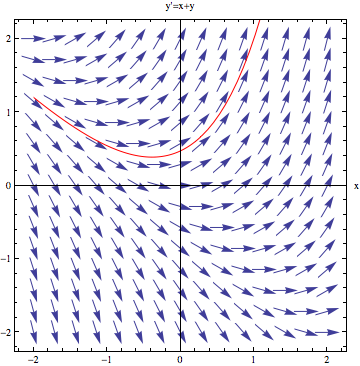
\includegraphics[width=.6\textwidth]{img/significato_geometrico_eq_diff.png}
	\end{figure}

	\noindent
	La ricerca delle primitive di una data funzione $f$, continua su un intervallo, equivale a risolvere l'equazione differenziale:
	\begin{equation*}
		y'=f\left(t\right)
	\end{equation*}
	che ha infinite soluzioni del tipo $y\left(t\right) = \displaystyle\int f\left(t\right) \:\mathrm{d}t + c, c \in \mathbb{R}$.

	Più in generale, l'\textbf{insieme delle soluzioni} di un'equazione differenziale di ordine $n$ o di un sistema di $n$ equazioni del primo ordine sia rappresentato da una famiglia di funzioni, \textbf{dipendente da $n$ parametri}. Tale famiglia prende il nome di \definition{integrale generale}.\newpage


	%%%%%%%%%%%%%%%%%%%%%
	% Equazioni lineari %
	%%%%%%%%%%%%%%%%%%%%%

	\subsection{Equazioni lineari}

	Le \definition{equazioni lineari} sono della forma:
	\begin{equation}\label{eq: forma equazioni lineari}
		y'\left(t\right) + a_{0}\left(t\right)y\left(t\right) = g\left(t\right)
	\end{equation}
	Con $a_{0}$ e $g$ funzioni reali di una variabile reale continue nel loro insieme di definizione, ossia:
	\begin{equation*}
		a_{0}, g \: : \: I \subseteq \mathbb{R} \rightarrow \mathbb{R}, \hspace{2em} a_{0}, g \in C^{0}\left(I\right)
	\end{equation*}
	L'\definition{integrale generale} dell'equazione differenziale lineare è data dalla formula:
	\begin{equation*}
		y\left(t\right) = e^{A\left(t\right)} \left[c_{1} + \displaystyle\int\left(g\left(t\right) e^{A\left(t\right)}\right) \: \mathrm{d}t \right]
	\end{equation*}
	In cui:
	\begin{equation*}
		A\left(t\right) = \displaystyle\int \left(a_{0}\left(t\right)\right) \:\mathrm{d}t
	\end{equation*}
	Attenzione, prima di applicare la formula, è importante avere la forma dell'equazione \ref{eq: forma equazioni lineari}.

	\begin{flushleft}
		\example{\underline{Esempio}}
	\end{flushleft}
	Data l'equazione:
	\begin{equation*}
		y' = y + x
	\end{equation*}
	Si porta nella forma dell'equazione \ref{eq: forma equazioni lineari}:
	\begin{equation*}
		y' - y = x
	\end{equation*}
	Si calcola l'integrale:
	\begin{equation*}
		e^{\int -1 \: \mathrm{d}x} \rightarrow -\displaystyle\int 1 \: \mathrm{d}x = -x \rightarrow e^{-x}
	\end{equation*}
	Si moltiplica il termine per entrambi i lati:
	\begin{equation*}
		\left(e^{-x}\right) y' + \left(-1 \cdot e^{-x}\right)y = x e^{-x}
	\end{equation*}
	E risulta evidente che adesso è possibile applicare la proprietà delle moltiplicazioni delle derivate:
	\begin{equation*}
		\begin{array}{rcl}
			\left[f\left(x\right) \cdot g\left(x\right)\right]' &=& f'\left(x\right) \cdot g\left(x\right) + f\left(x\right) \cdot g'\left(x\right) \\ [.3em]
			%
			\left(-1 \cdot e^{-x}\right)y + \left(e^{-x}\right) y' &=& \left[e^{-x} \cdot y\right]'
		\end{array}
	\end{equation*}
	Sostituendo il risultato, ottenuto eseguendo manipolazioni algebriche, all'interno dell'equazione:
	\begin{equation*}
		\left[\left(e^{-x}\right) y\right]' = x e^{-x}
	\end{equation*}
	A questo punto si esegue l'integrale:
	\begin{equation*}
		\displaystyle\int \left[\left(e^{-x}\right) y\right]' \:\mathrm{d}x = \displaystyle\int x e^{-x} \: \mathrm{d}x
	\end{equation*}
	A sinistra si può sempre semplificare la derivata con l'integrale, per cui non ci sono problemi:
	\begin{equation*}
		\left(e^{-x}\right) y = \displaystyle\int x e^{-x} \: \mathrm{d}x
	\end{equation*}
	A destra, si esegue il metodo per parti (par. \ref{subsubsection: integrare per parti}):
	\begin{gather*}
		f = x \hspace{1em} g' = e^{-x} \hspace{1em} f' = 1 \hspace{1em} g = -e^{-x} \\
		x \cdot \left(- e^{-x}\right) - \displaystyle\int 1 \cdot \left(- e^{-x}\right) \: \mathrm{d}x \\
		x \cdot \left(- e^{-x}\right) - \left(e^{-x}\right)
	\end{gather*}
	Dunque il risultato finale è:
	\begin{equation*}
		\begin{array}{rcl}
			\left(e^{-x}\right) y &=& -x e^{-x} - e^{-x} + c \\ [.3em]
			\left(e^{-x}\right) y &=& e^{-x}\left(-x - 1\right) + c \\ [1em]
			y &=& -x-1 + c \cdot \dfrac{1}{e^{-x}} \\ [1em]
			y &=& -x-1 + c \cdot e^{x}
		\end{array}
	\end{equation*}\newpage


	%%%%%%%%%%%%%%%%%%%%%%%%%%%%%%%%%%%%
	% Equazioni a variabili separabili %
	%%%%%%%%%%%%%%%%%%%%%%%%%%%%%%%%%%%%
	\subsection{Equazioni a variabili separabili}\label{subsection: equazioni a variabili separabili}

	Le \definition{equazioni a variabili separabili} sono della forma:
	\begin{equation}\label{eq: equazione a variabili separabili}
		y' = f\left(t\right)g\left(y\right)
	\end{equation}
	Con la funzione $f$ continua nell'intervallo $I$ ($f \in C\left(I\right)$) e la funzione $g$ continua nell'intervallo $J$ ($g \in C\left(J\right)$). Gli intervalli $I,J$ sono contenuti in $\mathbb{R}$.\newline

	\noindent
	\textbf{Nota bene:} se la funzione $\overline{y}$ è soluzione dell'equazione $g\left(y\right) = 0$, la retta $y = \overline{y}$ è una curva integrale (si veda l'esempio sottostante per convincersi di ciò).\newline

	\noindent
	Se $g\left(y\right) \ne 0$ in $J' \subseteq J$, l'integrale generale dell'equazione \ref{eq: equazione a variabili separabili} è:
	\begin{equation}\label{eq: integrale generale eq. a variabili separabili}
		\displaystyle\int \dfrac{1}{g\left(y\right)} \:\mathrm{d}y = \int f\left(t\right) \: \mathrm{d}t + c
	\end{equation}

	\begin{flushleft}
		\example{\underline{Esempio}}
	\end{flushleft}

	\noindent
	Data l'equazione:
	\begin{equation*}
		y' = 2t \sqrt{1-y^{2}}
	\end{equation*}
	Si può effettuare immediatamente un'osservazione importante. Come detto precedentemente, se $g\left(y\right) = 0$ e $\overline{y}$ è soluzione dell'equazione, allora $y = \overline{y}$ è una curva integrale. Si può facilmente trovare due valori di $y$ tali per cui l'equazione sia uguale a zero:
	\begin{equation*}
		\begin{array}{rcl}
			y = 1 & \longrightarrow & y' = 2t \sqrt{1 - 1^{2}} \\
				  &					& y' = 2 t \cdot 0 \\
				  &					& y' = 0 \\ [1em]
			y = -1& \longrightarrow & y' = 2t \sqrt{1 - \left(-1\right)^{2}} \\
				  & 				& y' = 2t \cdot 0 \\
				  &					& y' = 0
		\end{array}
	\end{equation*}
	Dato che:
	\begin{equation*}
		\begin{array}{rcl}
			f\left(t\right) &=& 2t \\
			g\left(y\right) &=& \sqrt{1-y^{2}}
		\end{array}
	\end{equation*}
	E con $y = \pm 1$ la funzione $g$ si annulla, allora $\pm 1$ sono soluzioni dell'equazione.\newline

	\noindent
	Adesso si cercano le soluzioni tali che $g\left(y\right) \ne 0$, quindi con $y \ne \pm 1$. Per farlo, si applica semplicemente la \dquotes{formula} \ref{eq: integrale generale eq. a variabili separabili}:
	\begin{equation*}
		\displaystyle\int \dfrac{1}{\sqrt{1-y^{2}}} \: \mathrm{d}y = 2 \displaystyle\int t \: \mathrm{d}t + c
	\end{equation*}
	Si procede con la risoluzione degli integrali:
	\begin{equation*}
		\begin{array}{rcl}
			\displaystyle 2 \cdot \int t \: \mathrm{d}t &=& 2 \cdot \dfrac{t^{2}}{2} = t^{2} + c \\ [2em]
			%
			\displaystyle \int \dfrac{1}{\sqrt{1 - y^{2}}} \: \mathrm{d}y & = & \arcsin\left(y\right) \\
		\end{array}
	\end{equation*}
	Si riaggregano i risultati:
	\begin{equation*}
		\arcsin\left(y\right) = t^{2} + c
	\end{equation*}
	Si esplicita la $y$ ricordando le proprietà della trigonometria $\arcsin\left(y\right) = x \rightarrow \sin\left(x\right) = y$:
	\begin{equation*}
		y = \sin\left(t^{2} + c\right)
	\end{equation*}
	


	\newpage

	%%%%%%%%%%%%%%%%%%%%%%
	% Problema di Cauchy %
	%%%%%%%%%%%%%%%%%%%%%%
	\subsection{Problema di Cauchy}\label{subsection: problema di Cauchy}

	Il \definition{problema di Cauchy (o dei valori iniziali)} ha due forme:
	\begin{itemize}
		\item Equazioni scalari di ordine $n$, con l'obbiettivo di trovare $y$ di classe\footnote{Con questa notazione si indica che una funzione ha una derivata continua di grado $n$. Quindi dicendo che $y$ è di classe $C^{4}$, vuol dire che $y$, $y'$, $y''$, $y'''$, $y''''$ sono tutte funzioni continue.} $C^{n}$ tale che:
		\begin{equation*}
			\begin{cases}
				y^{\left(n\right)}\left(t\right) = f\left(t, y\left(t\right), y'\left(t\right), ..., y^{\left(n-1\right)}\left(t\right)\right) \\
				%
				y\left(\tau\right) = \xi_{0} \\
				%
				y'\left(\tau\right) = \xi_{1} \\
				%
				\vdots 
				%
				y^{\left(n-1\right)}\left(\tau\right) = \xi_{n-1}
			\end{cases}
		\end{equation*}
		essendo $\tau, \xi_{0}, \cdots, \xi_{n-1}$ costanti assegnate;

		\item Sistemi, con l'obbiettivo di trovare $y$ di classe $C^{1}$ tale che:
		\begin{equation*}
			\begin{cases}
				y'=f\left(t, y\left(t\right)\right) \\
				y\left(\tau\right) = \xi
			\end{cases}
		\end{equation*}
		essendo $\tau \in \mathbb{R}$ e $\xi \in \mathbb{R}^{n}$ assegnati.
	\end{itemize}
	Le equazioni $y^{\left(j\right)}\left(\tau\right) = \xi_{j}$ con $j =0, \cdots, j=n-1$, e $y\left(\tau\right) = \xi$, prendono il nome di \definition{condizioni iniziali}. Le soluzioni si intendono definite localmente, ovvero in un intorno dell'istante iniziale $\tau$.\newline

	\noindent
	Un \example{esempio} di problema di Cauchy:
	\begin{equation*}
		\begin{cases}
			z''\left(t\right) + 4z'\left(t\right) + 4z\left(t\right) = \left(t+1\right)^{2} \\
			z\left(0\right) = \frac{1}{8} \\
			z'\left(0\right) = -3
		\end{cases}
	\end{equation*}

	\noindent
	Si consideri il seguente problema di Cauchy:
	\begin{equation*}
		(P)\begin{cases}
			y'\left(x\right) = a\left(x\right) b\left(y\right) \\
			y\left(x_{0}\right) = y_{0}
		\end{cases}
	\end{equation*}
	\begin{theorem}[\textbf{Teorema di esistenza e unicità locale per equazioni differenziabili a variabili separabili}]\label{theorem: teorema di esistenza e unicità locale per equazioni differenziabili a variabili separabili}
		Sia $a\left(x\right)$ una funzione continua in un intervallo aperto $I$ che contiene $x_{0}$ e $b\left(y\right)$ una funzione continua in un intervallo aperto $J$ che contiene $y_{0}$. Allora esiste $\delta > 0$ e una funzione definita per ogni $x \in I' \left[x_{0} - \delta, x_{0} + \delta\right] \subseteq I$ e ivi derivabile che risolve il problema di Cauchy. Se $b\left(y\right) \in C^{1}\left(J\right)$, allora tale soluzione unica.
	\end{theorem}

	\noindent
	Considerando il teorema \ref{theorem: teorema di esistenza e unicità locale per equazioni differenziabili a variabili separabili} enunciato poco fa, si intende dire che esiste almeno una funzione ($\overline{y}\left(x\right)$) tale che la sua derivata è uguale alla funzione continua ($a\left(x\right)$) moltiplicata per un'altra funzione continua ($b\left(y\right)$) che ha come parametro la primitiva:
	\begin{equation*}
		\begin{array}{rcl}
			\text{Primitiva} 	&\longrightarrow& \overline{y}\left(x\right) \\
			\text{Derivata}		&\longrightarrow& \overline{y}'\left(x\right) = a\left(x\right) \cdot b\left(\overline{y}\left(x\right)\right) \hspace{1em} \forall x \in \left[x_{0} - \delta, x_{0} + \delta \right]
		\end{array}
	\end{equation*}
	Ovviamente la derivata $\overline{y}\left(x\right)$ deve valere per qualsiasi $x$ che appartiene all'intorno $x_{0}$ aggiungendo/rimuovendo $\delta$. Inoltre la primitiva nel punto $x_{0}$ deve essere uguale a $y_{0}$ ($\overline{y}\left(x_{0}\right) = y_{0}$). Allora, la primitiva ($\overline{y}\left(x\right)$) è derivabile e la sua derivata è continua. L'unicità è possibile affermarla se la funzione $b\left(y\right)$ ha una proprietà più forte della continuità, ovvero la continuità nella derivata in $J$.

	\begin{boxdef}
		\definition{Teorema di esistenza e unicità globale per equazioni differenziali lineari.}\newline

		Si consideri l'equazione differneziale lineare
		\begin{equation*}
			y'\left(x\right) + a\left(x\right) \cdot y\left(x\right) = b\left(x\right)
		\end{equation*}
		Con $a\left(x\right)$ e $b\left(x\right)$ funzioni continue su un intervallo $I$ della retta reale. Se $x_{0} \in I$, allora il problema:
		\begin{equation*}
			\begin{cases}
				y'\left(x\right) + a\left(x\right) \cdot y\left(x\right) = b\left(x\right) & x \in I \\
				y\left(x_{0}\right) = y_{0}
			\end{cases}
		\end{equation*}
		Ammette un'unica soluzione in $I$.
	\end{boxdef}
	
	\begin{boxdef}
		\definition{Struttura dell'insieme delle soluzioni di un'equazione omogenea del primo ordine.}\newline

		L'insieme $V$ delle soluzioni dell'equazione omogenea
		\begin{equation*}
			y' + a\left(x\right)y = 0
		\end{equation*}
		È uno spazio vettoriale su $\mathbb{R}$ di dimensione $1$.

		Indicando con $y_{P}\left(x\right)$ una soluzione particolare dell'equazione completa
		\begin{equation*}
			y' + a\left(x\right) y = b\left(x\right)
		\end{equation*}
		Allora il suo integrale generale è
		\begin{equation*}
			y\left(x\right) = y_{P}\left(x\right) + y_{om}\left(x\right) \hspace{1em} y_{om}\left(x\right) \in V
		\end{equation*}
	\end{boxdef}\newpage

	\subsubsection{Intervallo massimale}\label{subsubsection: intervallo massimale}

	Si parte subito con il dire che determinare l'intervallo massimale non è un'operazione banale. Questo perché non esistono algoritmi (semplici) certi che consentono di ottenere un intervallo massimale. Tuttavia, lo studente può utilizzare il ragionamento ed eventuali intuizioni per capire quando una soluzione ha intervallo estendibile e quando esso è massimale.

	\begin{boxdef}
		Il più ampio intervallo su cui la soluzione è definita si chiama \definition{intervallo massimale}.
	\end{boxdef}

	\noindent
	L'intervallo massimale è possibile determinarlo una volta che si è giunti al termine del problema di Cauchy (par. \ref{subsection: problema di Cauchy}). Una volta concluso l'esercizio, avendo trovato l'integrale generale e la costante $c$, è necessario eseguire alcuni passaggi:
	\begin{enumerate}[label=\alph*)]
		\item Nell'integrale generale, sostituire la costante $c$ trovata al termine dell'esercizio;
		\item Esplicitare la $y$ tramite passaggi algebrici;
		\item Porre la condizione di esistenza;
		\item Studiare l'intervallo massimale con appositi ragionamenti.
	\end{enumerate}
	Si procede presentando due esempi e ricordando che un intervallo, \underline{\textbf{può}} essere esteso se rispetta certe condizioni.

	\begin{flushleft}
		\example{\underline{Esempio 1}}
	\end{flushleft}

	\noindent
	Dato il seguente problema di Cauchy:
	\begin{equation*}
		\begin{cases}
			y' = \sqrt{y}e^{-x} \\
			y\left(0\right) = 1
		\end{cases}
	\end{equation*}
	Calcolare l'intervallo massimale.\newline

	\noindent
	Il problema è risolvibile con il metodo delle variabili separabili (par. \ref{subsection: equazioni a variabili separabili}):
	\begin{equation*}
		\begin{array}{rcl}
			y'\left(x\right) &=& f\left(x\right) g\left(y\right) \\
			f\left(x\right) &=& e^{-x} \\
			g\left(y\right) &=& \sqrt{y} \\ [1em]
			\displaystyle\int \dfrac{1}{\sqrt{y}} \: \mathrm{d}y &=& \displaystyle\int e^{-x} \: \mathrm{d}x + c
		\end{array}
	\end{equation*}
	Si potrebbe tentare di calcolare una soluzione costante, ma risulterebbe evidente che l'unica soluzione costante, cioè $y = 0$, non è ammessa come soluzione del problema (condizione iniziale $y\left(0\right) = 1$!). Per questo motivo, si procede con il metodo delle variabili separabili.\newline

	\noindent
	Si risolve l'integrale:
	\begin{equation*}
		\begin{array}{rcl}
			\displaystyle\int y^{-\frac{1}{2}} \: \mathrm{d}y &=& -e^{-x} + c \\ [1em]
			%
			&\downarrow& \text{si utilizza l'integrale notevole } \displaystyle\int x^{n} \: \mathrm{d}x = \dfrac{x^{n+1}}{n+1} \hspace{1em} n \ne -1 \\ [1em]
			%
			\dfrac{y^{\frac{1}{2}}}{\dfrac{1}{2}} &=& -e^{-x} + c \\ [2.5em]
			%
			2\sqrt{y} &=& -e^{-x} + c
		\end{array}
	\end{equation*}
	La soluzione trovata è l'integrale generale. Si conclude il problema di Cauchy trovando la costante $c$, quindi applicando la condizione iniziale $y\left(0\right) = 1$:
	\begin{equation*}
		\begin{array}{rcl}
			2\sqrt{1} &=& -e^{-0} + c \\
			2 + 1 &=& c \\
			3 &=& c
		\end{array}
	\end{equation*}
	Adesso si calcola l'intervallo massimale:
	\begin{itemize}
		\item Si sostituisce nell'integrale generale la costante $c$:
		\begin{equation*}
			2\sqrt{y} = -e^{-x} + 3
		\end{equation*}
		Si esplicita la $y$:
		\begin{equation*}
			\begin{array}{rcl}
				\sqrt{y} &=& -\dfrac{e^{-x}}{2} + \dfrac{3}{2} \\ [.5em]
				y &=& \left(-\dfrac{e^{-x}}{2} + \dfrac{3}{2}\right)^{2}
			\end{array}
		\end{equation*}

		\item Le condizioni d'esistenza del problema di Cauchy sono le seguenti:
		\begin{equation*}
			\sqrt{y}e^{-x} \hspace{1em} \longrightarrow \hspace{1em} \underbrace{\left]-\infty, +\infty\right[}_{def. x} \times \overbrace{\left[0, +\infty \right[}^{def. y}
		\end{equation*}
		La $y$ deve essere maggiore/uguale a zero, mentre la $x$ non ha grosse restrizioni. L'intervallo massimale per definizione può essere identico o un sottoinsieme. Per trovarlo è necessario studiare il valore della $y$ esplicitata al passaggio precedente. In questo caso, essa in zero ($y=0$) non ha soluzione, per cui si cercano le soluzioni per $y > 0$.

		\item Andando a cercare una soluzione costante dell'equazione differenziale, ci si accorge che $g\left(y\right) = \sqrt{y}$ è uguale a zero solo se $y = 0$, e quindi essa sarebbe una soluzione costante del problema (ricordandosi quanto detto nel par. \ref{subsection: equazioni a variabili separabili}) poiché $g\left(y\right) = 0$ con $y = \overline{y}$. Tuttavia, $y = 0$ non è ammesso dal problema a causa della condizione iniziale $y\left(0\right) = 1$. 
		
		Per questo motivo, si cerca una soluzione tale che $y > 0$. E per farlo, si prende in considerazione la $y$ trovata al passaggio precedente e si impone una condizione:
		\begin{equation*}
			\begin{array}{rcl}
				-\dfrac{e^{-x}}{2} + \dfrac{3}{2} &>& 0 \\ [1em]
				-e^{-x} &>& -3 \\ [.3em]
				e^{-x} &<& 3 \\ [.3em]
				-x &<& \ln\left(3\right) \\ [.3em]
				x &>& -\ln\left(3\right)
			\end{array}
		\end{equation*}

		\item Per ciascun valore di $x$ che è maggiore di $-\ln\left(3\right)$, la $y$ deve valere:
		\begin{equation*}
			y = \left(-\dfrac{e^{-x}}{2} + \dfrac{3}{2}\right)^{2}
		\end{equation*}
		E per tutti gli altri casi? Nei casi in cui la $x$ sia minore o uguale a $-\ln\left(3\right)$, la $y$ dovrà valere $0$, come confermato nel caso della soluzione costante $y = 0$.

		Da queste considerazioni, è possibile rappresentare la soluzione del problema di Cauchy $\overline{y}$ come:
		\begin{equation*}
			\overline{y}\left(x\right) = \begin{cases}
				\left(-\dfrac{e^{-x}}{2} + \dfrac{3}{2}\right)^{2} 	& \text{se } x > -\ln\left(3\right) \\
				\\
				0													& \text{se } x \le -\ln\left(3\right)
			\end{cases}
		\end{equation*}
		Per cui l'intervallo massimale è $-\infty,+\infty$ e difatti si può estendere a destra e sinistra.
	\end{itemize}

	\begin{flushleft}
		\example{\underline{Esempio 2}}
	\end{flushleft}

	\noindent
	Dato il seguente problema di Cauchy:
	\begin{equation*}
		\begin{cases}
			y'-y^{2}\cos\left(x\right) = 0 \\
			\\
			y\left(\dfrac{\pi}{2}\right) = -1
		\end{cases}
	\end{equation*}
	Calcolare l'intervallo massimale.\newline

	\noindent
	Il problema è risolvibile con il metodo delle variabili separabili (par. \ref{subsection: equazioni a variabili separabili}):
	\begin{equation*}
		\begin{array}{rcl}
			y'\left(x\right) - f\left(x\right) g\left(y\right) &=& 0 \longrightarrow y'\left(x\right) = f\left(x\right) g\left(y\right) \\
			f\left(x\right) &=& \cos\left(x\right) \\
			g\left(y\right) &=& y^{2} \\ [1em]
			\displaystyle\int \dfrac{1}{y^{2}} \: \mathrm{d}y &=& \displaystyle\int \cos\left(x\right) \: \mathrm{d}x + c
		\end{array}
	\end{equation*}
	Si potrebbe tentare di calcolare una soluzione costante, ma risulterebbe evidente che l'unica soluzione costante, cioè $y = 0$, non è ammessa come soluzione del problema (condizione iniziale $y\left(\frac{\pi}{2}\right) = -1$!). Per questo motivo, si procede con il metodo delle variabili separabili.\newline

	\noindent
	Si risolve l'integrale:
	\begin{equation*}
		\begin{array}{rcl}
			\displaystyle\int \dfrac{1}{y^{2}} \: \mathrm{d}y &=& \displaystyle\int \cos\left(x\right) \: \mathrm{d}x \\ [1em]
			%
			\displaystyle\int y^{-2} \: \mathrm{d}y &=& \displaystyle\int \cos\left(x\right) \: \mathrm{d}x \\ [1em]
			%
			&\downarrow& \text{si utilizza l'integrale notevole } \displaystyle\int x^{n} \:\mathrm{d}x = \dfrac{x^{n+1}}{n+1} \hspace{1em} n \ne -1 \\ [1em]
			%
			\dfrac{y^{-1}}{-1} &=& \sin\left(x\right) \\ [1em]
			%
			-y^{-1} &=& \sin\left(x\right) \\ [.5em]
			%
			y &=& -\dfrac{1}{\sin\left(x\right)} + c
		\end{array}
	\end{equation*}
	La soluzione trovata è l'integrale generale. Si conclude il problema di Cauchy trovando la costante $c$, quindi applicando la condizione iniziale $y\left(\frac{\pi}{2}\right)=-1$:
	\begin{equation*}
		\begin{array}{rcl}
			-1 &=& -\dfrac{1}{\sin\left(\frac{\pi}{2}\right)} + c \\ [1em]
			%
			-1 &=& -\dfrac{1}{1} + c \\ [1em]
			%
			0 &=& c
		\end{array}
	\end{equation*}\newpage

	\noindent
	Adesso si calcola l'intervallo massimale:
	\begin{itemize}
		\item Si sostituisce nell'integrale generale la costante $c$:
		\begin{equation*}
			y = -\dfrac{1}{\sin\left(x\right)} + 0
		\end{equation*}
		
		\item La condizione d'esistenza del problema di Cauchy sono le seguenti:
		\begin{equation*}
			y^{2}\cos\left(x\right) \hspace{1em} \longrightarrow \hspace{1em} \underbrace{\left] -\infty, +\infty \right[}_{def. x} \times \overbrace{\left] -\infty, +\infty \right[}^{def. y}
		\end{equation*}

		\item A differenza dell'esempio precedente, in questo caso la $x$ non può essere qualsiasi valore poiché c'è un $\sin$ al denominatore che potrebbe causare una divisione per zero (impossibile). Per cui, la condizione d'esistenza è:
		\begin{equation*}
			\sin\left(x\right) > 0
		\end{equation*}
		Calcolando il $\arcsin$ di $0$, si ottiene:
		\begin{equation*}
			x > \arcsin\left(0\right) \longrightarrow x > 0
		\end{equation*}
		Ma attenzione! Perché il valore $\sin$ si può annullare anche con altri valori di $x$, come per esempio $\pi$, per cui:
		\begin{equation*}
			0 < x < \pi
		\end{equation*}
		Questo risulta l'intervallo massimale, ovviamente estremi esclusi.
	\end{itemize}\newpage

	\subsubsection{Equazioni differenziali lineari del secondo ordine}\label{subsubsection: equazioni differenziali lineari del secondo ordine}

	Le \definition{equazioni differenziali lineari del secondo ordine} nella forma standard sono composte nel seguente modo:
	\begin{equation*}
		y''\left(x\right) + a\left(x\right)y'\left(x\right) + b\left(x\right)y\left(x\right) = f\left(x\right)
	\end{equation*}
	Con $a\left(x\right)$, $b\left(x\right)$, $f\left(x\right) \in \mathcal{C}^{0}\left(I\right)$.\newline

	\noindent
	Il problema di Cauchy per una equazione lineare del secondo ordine è composto nel seguente modo:
	\begin{equation*}
		\begin{cases}
			y''\left(x\right) + a\left(x\right)y'\left(x\right) + b\left(x\right)y\left(x\right) = f\left(x\right) \\
			y\left(x_{0}\right) = y_{0} \\
			y'\left(x_{0}\right) = v_{0}
		\end{cases}
	\end{equation*}
	
	\begin{boxdef}
		\definition{Teorema di esistenza e unicità globale per equazioni lineari del secondo ordine.}\newline
		
		Si consideri l'equazione differenziale lineare
		\begin{equation*}
			y''\left(x\right) + a\left(x\right) \cdot y'\left(x\right) + b\left(x\right) \cdot y\left(x\right) = f\left(x\right)
		\end{equation*}
		Con $a\left(x\right)$, $b\left(x\right)$ e $f\left(x\right)$ funzioni continue su un intervallo $I$ detta retta reale. Se $x_{0} \in I$, allora il problema:
		\begin{equation*}
			\begin{cases}
				y''\left(x\right) + a\left(x\right)y'\left(x\right) + b\left(x\right)y\left(x\right) = f\left(x\right) \\
				y\left(x_{0}\right) = y_{0} \\
				y'\left(x_{0}\right) = v_{0}
			\end{cases}
		\end{equation*}
		Ammette un'unica soluzione in $I$.
	\end{boxdef}

	\begin{boxdef}
		\definition{Struttura dell'insieme delle soluzioni di un'equazione omogenea del secondo ordine}\newline

		L'insieme $V$ delle soluzioni di un'equazione differenziale lineare omogenea del secondo ordine è uno spazio vettoriale su $\mathbb{R}$ di dimensione $2$.
	\end{boxdef}

	\noindent
	L'insieme $S$ delle soluzioni dell'equazione completa è una varietà lineare:
	\begin{equation*}
		S = \left\{y_{P}\left(x\right) + y_{om}\left(x\right) : y_{om}\left(x\right) \in V\right\}
	\end{equation*}
	In cui $y_{P}\left(x\right)$ è una soluzione particolare dell'equazione completa.\newline

	\noindent
	Per risolvere questo tipo di equazioni, si utilizza il \textbf{metodo di somiglianza o dei coefficienti indeterminati} (par. \ref{subsection: metodo di somiglianza o dei coefficienti indeterminati}).\newpage

	\subsection{Metodo di somiglianza o dei coefficienti indeterminati}\label{subsection: metodo di somiglianza o dei coefficienti indeterminati}
	Il metodo di somiglianza o dei coefficienti indeterminati è una tecnica che consente di risolvere le equazioni differenziali lineari del secondo ordine rapidamente.\\

	\noindent
	Non esiste un'unica tecnica risolutiva, ma è necessario avere a disposizione una serie di \textbf{\emph{pattern risolutivi}}. Il motivo è dovuto al fatto che ogniqualvolta si presenti un'equazione differenziale lineare del secondo grado, si eseguirà un \emph{matching} tra i \emph{pattern risolutivi} che si hanno a disposizione e l'equazione risultante (in parole povere, l'espressione a destra dell'uguale).\newline

	\begin{table}[!htp]
		\centering
		\begin{tabular}{@{} l l l @{}}
			\toprule
			\textbf{Tipo}	& \textbf{Equazione differenziale} & \textbf{Soluzione particolare} \\
			\midrule
			Monomio	& $y'' + y' - 2y = 5$ & $y_{P}\left(x\right) = a$ \\
			\cmidrule{1-3}
			Primo grado 	& $y'' + y' - 2y = x + 2$ & $y_{P}\left(x\right) = ax + b$ \\ 
			\cmidrule{1-3} 
			Secondo grado	& $y'' + 3y' + 2y = 2x^{2} - 1$ & $y_{P}\left(x\right) = ax^{2} + bx + c$ \\
			\cmidrule{1-3} 
			\multirow{4}{*}{Esponenziale} 	& $y'' + 3y' - 2y = 3e^{-x}$	& $y_{P}\left(x\right) = ae^{-x}$ \\ [.3em]
			& $y'' - 3y' + 2y = 3e^{-x} \cdot x$	& $y_{P}\left(x\right) = \left(ax + b\right) e^{-x}$ \\ [.3em]
			& $y'' - 3y' + 2y = 3e^{x}$	& $y_{P}\left(x\right) = x \cdot ae^{x}$ \\ [.3em]
			& $y'' - 3y' + 2y = 3e^{2x} \cdot x$	& $y_{P}\left(x\right) = \left(ax + b\right) e^{2x} \cdot x$ \\
			\cmidrule{1-3}
			Coseno/Seno 	& $y'' + y' = \cos\left(2x\right)$ & $y_{P}\left(x\right) = a \cdot \cos\left(2x\right) + b \cdot \sin\left(2x\right)$ \\
			\bottomrule
		\end{tabular}
		\caption{Pattern risolutivi del metodo di somiglianza.}
		\label{tab: pattern risolutivi del metodo di somiglianza}
	\end{table}

	\noindent
	A questi pattern è necessario aggiungere alcuni casi che modificano la soluzione particolare. \textbf{Attenzione:} questi casi modificano la soluzione particolare scelta! Nella tabella \ref{tab: casi particolari del metodo di somiglianza}, si indicano con $\lambda$ le soluzioni dell'equazione caratteristica (in parole povere l'equazione a sinistra dell'uguale).\newline

	\noindent
	Un altro caso particolare è il \textbf{principio di sovrapposizione}. In questo caso, basta risolvere ogni fattore come un'equazione a sé stante. Per cui la soluzione particolare si compone nel seguente modo:
	\begin{equation*}
		y_{P}\left(x\right) = y_{P_{1}}\left(x\right) + y_{P_{2}}\left(x\right)
	\end{equation*}
	Per esempio, data l'equazione:
	\begin{equation*}
		y'' + 6y' + 8y = e^{2x} + \sqrt{\pi} x^{2}
	\end{equation*}
	Si risolve:
	\begin{equation*}
		y'' + 6y' + 8y = e^{2x}
	\end{equation*}
	E successivamente:
	\begin{equation*}
		y'' + 6y' + 8y = \sqrt{\pi} x^{2}
	\end{equation*}\newpage

	\begin{table}[!htp]
		\centering
		\begin{tabular}{@{} c c c @{}}
			\toprule
			$\boldsymbol{\lambda}$ & \textbf{Equazione differenziale} & \textbf{Che cosa viene modificato} \\
			\midrule
			%
			\multicolumn{3}{p{32em}}{\framedtext{Nel caso in cui la soluzione dell'equazione caratteristica è uguale a zero, si moltiplica la \textbf{soluzione particolare} per $x$. Quest'ultima viene elevata ad un valore pari al numero di volte che essa annulla l'equazione caratteristica.
			
			Nell'esempio sottostante, la $x$ viene elevata ad $1$ poiché le soluzioni dell'equazione caratteristica sono $\lambda_{1} = 0$ e $\lambda_{2} = -1$. Dunque, $\lambda_{1}$ annulla soltanto una volta l'equazione caratteristica (chiamata formalmente molteplicità algebrica).
			
			\underline{Attenzione:} la regola viene applicata solo ai polinomi di primo e secondo grado.}}\\\\
			$\lambda = 0$ & $y''+y' = x+2$ & $y_{P}\left(x\right) = \left(ax+b\right)x^{1}$ \\ [.5em]
			%
			\cmidrule{1-3}
			%
			\multicolumn{3}{p{32em}}{\framedtext{Nel caso in cui le soluzioni dell'equazione caratteristica siano uguale tra di loro, si modifica la \textbf{soluzione generale} aggiungendo una $x$.
			
			Nell'esempio sottostante, le soluzioni dell'equazione caratteristica sono $\lambda_{1} = \lambda_{2} = 1$ per cui viene aggiunta una $x$ nella soluzione generale.}} \\\\
			$\lambda_{1} = \lambda_{2}$ & $y'' - 2y' + y = \left(x - 1\right)^{2}$ & $y\left(x\right) = y_{P}\left(x\right) + c_{1}e^{x} + c_{2}e^{x} \cdot x$ \\ [.5em]
			%
			\cmidrule{1-3}
			%
			\multicolumn{3}{p{32em}}{\framedtext{Nel caso in cui le soluzioni dell'equazione caratteristica siano uguali al termine dell'esponenziale ($e^{\alpha x}$) presente a destra dell'uguale dell'equazione caratteristica, alla \textbf{soluzione particolare} viene moltiplicata una $x$ elevata ad un valore pari alla sua molteplicità algebrica.
			
			Nell'esempio sottostante, le soluzioni dell'equazione caratteristica sono $\lambda_{1} = $ e $\lambda_{2} = $. E dato che il valore di $\lambda_{n}$ compare nell'esponenziale dell'equazione caratteristica, viene aggiunta una $x$.
			
			\underline{Attenzione:} la regola vale solo se l'esponenziale ha una $x$ tra i suoi termini, quindi non è valida per esempio con $e^{2}$. In generale deve essere: $e^{\alpha x}$}} \\\\
			$\lambda_{1} = \alpha$ & $y'' - 5y' + 6y = 3x e^{2x}$ & $y_{P}\left(x\right) = x \cdot \left[e^{2x}\left(ax+b\right)\right]$ \\ [.5em]
			%
			\cmidrule{1-3}
			%
			\multicolumn{3}{p{32em}}{\framedtext{Nel caso in cui le soluzioni dell'equazione caratteristica siano numeri immaginari e uguali: al termine dell'esponenziale ($e^{\alpha x}$) e al termine del seno/coseno ($\cos\left(\beta x\right)$/$\sin\left(\beta x\right)$); allora viene aggiunta una $x$ alla \textbf{soluzione particolare}.}} \\\\
			\multirow{2}{*}{$\lambda = \alpha \pm \beta i$} & $y'' \cdots = e^{\alpha x} \cos\left(\beta x\right)$ & \multirow{2}{*}{$y_{P}\left(x\right) = x \cdot e^{\alpha x}\left(\cos\left(\beta x\right) + \sin\left(\beta x\right)\right)$} \\
			& $y'' \cdots = e^{\alpha x} \sin\left(\beta x\right)$ & \\
			\bottomrule
		\end{tabular}
		\caption{Casi particolari della $\lambda$ nel metodo di somiglianza.}
		\label{tab: casi particolari del metodo di somiglianza}
	\end{table}\newpage

	% TODO: add examples

	\subsection{Metodo di variazione delle costanti}

	Il \definition{metodo di variazione} delle costanti è una tecnica più generale che consente di ricavare una soluzione particolare dell'equazione completa, qualunque sia la forma del termine forzante (cioè quello a destra dell'uguale).\newline

	\noindent
	Data l'equazione differenziale lineare del secondo ordine:
	\begin{equation*}
		y'' + ay' + by = f\left(x\right)
	\end{equation*}
	Dopo aver ottenuto la soluzione particolare con il metodo di somiglianza (par. \ref{subsection: metodo di somiglianza o dei coefficienti indeterminati}):
	\begin{equation*}
		y_{P}\left(x\right) = c_{1}\left(x\right)y_{1}\left(x\right) + c_{2}\left(x\right) y_{2}\left(x\right)
	\end{equation*}
	Si possono ottenere le due costanti grazie a queste operazioni tra matrici:
	\begin{equation*}
		\underbrace{
			\begin{bmatrix}
				y_{1}\left(x\right) & y_{2}\left(x\right) \\
				y_{1}'\left(x\right) & y_{2}'\left(x\right)
			\end{bmatrix}
		}_{Wronskiana}
		\cdot
		\begin{bmatrix}
			c_{1}'\left(x\right) \\
			c_{2}'\left(x\right)
		\end{bmatrix}
		=
		\begin{bmatrix}
			0 \\
			f\left(x\right)
		\end{bmatrix}
	\end{equation*}
	Attenzione, in questo caso le costanti sono derivate, per cui è necessario integrarle per ottenere la soluzione finale.

	\begin{flushleft}
		\example{\underline{\textbf{Esempio}}}
	\end{flushleft}

	\noindent
	Determinare l'integrale generale dell'equazione:
	\begin{equation*}
		y'' + y = \sin\left(x\right)
	\end{equation*}
	Le soluzioni dell'equazione caratteristica sono:
	\begin{equation*}
		\dfrac{-0 \pm \sqrt{0^{2} - 4 \cdot 1 \cdot 1}}{2} = \dfrac{\pm\sqrt{-4}}{2} = \dfrac{\pm2i}{2} = \pm i
	\end{equation*}
	La soluzione generale dunque è:
	\begin{equation*}
		y\left(x\right) = y_{P}\left(x\right) + c_{1} e^{i \cdot x} + c_{2} e^{-i \cdot x}
	\end{equation*}
	Per ottenere la soluzione particolare viene utilizzato il metodo di somiglianza:
	\begin{equation*}
		y_{P}\left(x\right) = a \cdot \cos\left(x\right) + b \cdot \sin\left(x\right)
	\end{equation*}
	Adesso viene utilizzato il metodo di variazione per ottenere le costanti. Quindi si costruiscono le matrici:
	\begin{equation*}
		\begin{array}{rcl}
			\begin{bmatrix}
				y_{1}\left(x\right) & y_{2}\left(x\right) \\
				y_{1}'\left(x\right) & y_{2}'\left(x\right)
			\end{bmatrix}
			\cdot
			\begin{bmatrix}
				a'\left(x\right) \\
				b'\left(x\right)
			\end{bmatrix}
			&=&
			\begin{bmatrix}
				0 \\
				f\left(x\right)
			\end{bmatrix} \\ [1em]
			%
			\begin{bmatrix}
				\cos\left(x\right) & \sin\left(x\right) \\
				-\sin\left(x\right) & \cos\left(x\right)
			\end{bmatrix}
			\cdot
			\begin{bmatrix}
				a' \\ b'
			\end{bmatrix}
			&=&
			\begin{bmatrix}
				0 \\ \sin\left(x\right)
			\end{bmatrix} \\ [.8em]
			%
			\begin{bmatrix}
				a' \\ b'
			\end{bmatrix}
			&=&
			\begin{bmatrix}
				\cos\left(x\right) & -\sin\left(x\right) \\
				\sin\left(x\right) & \cos\left(x\right)
			\end{bmatrix}^{-1}
			\cdot
			\begin{bmatrix}
				0 \\ \sin\left(x\right)
			\end{bmatrix} \\ [1em]
			%
			\begin{bmatrix}
				a' \\ b'
			\end{bmatrix}
			&=&
			\begin{bmatrix}
				- \sin^{2}\left(x\right) \\
				\cos\left(x\right) \sin\left(x\right)
			\end{bmatrix}
		\end{array}
	\end{equation*}\newpage

	\noindent
	Per ottenere le costanti $a$ e $b$ è necessario integrare le derivate appena trovare, per cui:
	\begin{equation*}
		\begin{array}{rcl}
			a &=& \displaystyle\int -\sin^{2}\left(x\right) \:\mathrm{d}x \\
			%
			&\downarrow& \text{si utilizza l'integrale fondamentale } \displaystyle\int \sin^{2}\left(x\right) \: \mathrm{d}x = \int\dfrac{1-\cos\left(2x\right)}{2} \: \mathrm{d}x \\ [1em]
			%
			&=& - \displaystyle\int \dfrac{1-\cos\left(2x\right)}{2} \:\mathrm{d}x \\ [1em]
			%
			&=& -\displaystyle\int \dfrac{1}{2} - \dfrac{\cos\left(2x\right)}{2} \:\mathrm{d}x \\ [1em]
			%
			&=& \displaystyle -\left( \int\dfrac{1}{2} \:\mathrm{d}x - \int \dfrac{\cos\left(2x\right)}{2} \:\mathrm{d}x \right) \\ [1em]
			%
			&=& \displaystyle -\left( \dfrac{1}{2}x - \dfrac{1}{2}\cdot\int\cos\left(2x\right) \:\mathrm{d}x \right) \\ [1em]
			%
			&\downarrow& \text{si ricorda il risultato della seguente derivata } \dfrac{\mathrm{d}}{\mathrm{d} x} \sin\left(5x\right) = 5\cos\left(5x\right) \\ [1em]
			%
			&=& -\dfrac{1}{2}x -\left(-\dfrac{1}{2} \cdot \dfrac{\sin\left(2x\right)}{2}\right) \\ [1em]
			%
			&=& -\dfrac{1}{2}x + \dfrac{\sin\left(2x\right)}{4} \\ [3em]
			%
			%~~~~~~~~~~~~~~~~~~~~~~~~~~~~~~~~~~~~~~~~~~%
			%
			b &=& \displaystyle\int \cos\left(x\right)\sin\left(x\right) \: \mathrm{d}x \\
			%
			&\downarrow& \text{si utilizza il metodo di sostituzione } t = \sin\left(x\right) \hspace{1em} \mathrm{d}x = \dfrac{1}{t'} \: \mathrm{d}t \\ [1em]
			%
			&=& \displaystyle\int \cos\left(x\right) \cdot t \cdot \dfrac{1}{\cos\left(x\right)} \: \mathrm{d}t \\ [1em]
			%
			&=& \displaystyle\int \cancel{\cos\left(x\right)} \cdot t \cdot \dfrac{1}{\cancel{\cos\left(x\right)}} \: \mathrm{d}t \\ [1em]
			%
			&=& \displaystyle\int t \: \mathrm{d}t \\ [1em]
			%
			&=& \dfrac{t^{2}}{2} \\ [1em]
			%
			&\downarrow& \text{si conclude il metodo di sostituzione} \\ [1em]
			%
			&=& \dfrac{\sin^{2}\left(x\right)}{2} + c
		\end{array}
	\end{equation*}
	Per cui, andando a sostituire i due risultati nella soluzione particolare, è possibile ottenere anche la soluzione generale:
	\begin{equation*}
		\begin{array}[pos]{rcl}
			y_{P}\left(x\right) &=& \left(-\dfrac{1}{2}x + \dfrac{\sin\left(2x\right)}{4}\right)\cos\left(x\right) + \left(\dfrac{\sin^{2}\left(x\right)}{2}\right)\sin\left(x\right) \\ [1.4em]
			%
			y\left(x\right) &=& y_{P}\left(x\right) + c_{1} e^{i \cdot x} + c_{2} e^{-i \cdot x}
		\end{array}
	\end{equation*}\newpage

	\subsection{Sistemi di equazioni differenziali}\label{subsection: sistemi di equazioni differenziali}

	Nel corso di Analisi II vengono affrontati sistemi lineari del primo ordine a coefficienti costanti, quindi nella forma del tipo:
	\begin{equation*}
		\begin{cases}
			x\left(t\right) = ax\left(t\right) + by\left(t\right) + f_{1}\left(x\right) \\
			y'\left(t\right) = cx\left(t\right) + dy\left(t\right) + f_{2}\left(x\right)
		\end{cases}
	\end{equation*}
	Dove $a,b,c,d \in \mathbb{R}$ e $x \in I$.\newline

	\noindent
	La \textbf{risoluzione} dei \definition{sistemi di equazioni differenziali} prevede di risolvere la seguente equazione matriciale:
	\begin{equation}\label{eq: sistemi di equazioni differenziali}
		\begin{array}{rcl}
			\mathbf{X}' &=& A\mathbf{X} + \mathbf{F} \\ [1em]
			%
			\begin{bmatrix}
				x' \\ y'
			\end{bmatrix}
			&=&
			\begin{bmatrix}
				a & b \\ c & d
			\end{bmatrix}
			\cdot
			\begin{bmatrix}
				x \\ y
			\end{bmatrix}
			+
			\begin{bmatrix}
				f_{1}\left(x\right) \\
				f_{2}\left(x\right)
			\end{bmatrix}
		\end{array}
	\end{equation}
	Nel caso i valori $f_{1}\left(x\right)$ e $f_{2}\left(x\right)$ siano nulli, cioè uguali a zero, il sistema viene detto \textbf{omogeneo}:
	\begin{equation*}
		\mathbf{X}' = A \mathbf{X}
	\end{equation*}
	In questo caso, calcolando gli autovalori (vedere esempio a fine paragrafo se non si ricorda come calcolare gli autovalori) della matrice $A$: 
	\begin{equation*}
		\det\left(A - \lambda \cdot I\right) = 0 \rightarrow
		\det\left(
			\begin{bmatrix}
				a & b \\ c & d
			\end{bmatrix}
			-
			\lambda \cdot \begin{bmatrix}
				1 & 0 \\ 0 & 1
			\end{bmatrix}
		\right) = 0
	\end{equation*}
	è possibile trovare una forma dell'integrale generale particolare. Si ricorda che il determinante di una matrice quadrata $2 \times 2$ è possibile calcolarlo eseguendo una somma tra la moltiplicazione dei valori della diagonale principale e tra la moltiplicazione dei valori della diagonale secondaria.

	\begin{boxdef}
		Siano $\lambda_{1}$ e $\lambda_{2}$ due autovalori distinti della matrice $A$ del sistema omogeneo e siano $\mathbf{K}_{1}$ e $\mathbf{K}_{2}$ i corrispondenti autovettori. Dunque, l'integrale generale di un sistema di equazioni differenziali sull'intervallo $\left(-\infty, + \infty\right)$ è dato da:
		\begin{equation*}
			\mathbf{X} = c_{1} \mathbf{K}_{1} e^{\lambda_{1}t} + c_{2} \mathbf{K}_{2} e^{\lambda_{2}t}
		\end{equation*}
	\end{boxdef}\newpage

	\begin{flushleft}
		\example{\underline{Esempio}}
	\end{flushleft}

	\noindent
	Risolvere il seguente sistema:
	\begin{equation*}
		\begin{cases}
			x'\left(t\right) = 2x\left(t\right) + 3y\left(t\right) \\
			y'\left(t\right) = 2x\left(t\right) + y\left(t\right)
		\end{cases}
	\end{equation*}
	Innanzitutto, si può osservare immediatamente che è un sistema omogeneo poiché mancano i termini $f_{1,2}\left(x\right)$ (vedi l'eq. \ref{eq: sistemi di equazioni differenziali}). Si procede con la costruzione della matrice $A$ e il calcolo dei suoi autovalori:
	\begin{gather*}
		A = \begin{bmatrix}
			2 & 3 \\ 2 & 1
		\end{bmatrix} \\
		%
		\begin{array}{rcl}
			\det\left(
				\begin{bmatrix}
					2 & 3 \\ 2 & 1
				\end{bmatrix}
				-
				\lambda
				\begin{bmatrix}
					1 & 0 \\ 0 & 1
				\end{bmatrix}
			\right) &=& 0 \\ [1.5em]
			%
			\det\left(
				\begin{bmatrix}
					2 & 3 \\ 2 & 1
				\end{bmatrix}
				-
				\begin{bmatrix}
					\lambda & 0 \\ 0 & \lambda
				\end{bmatrix}
			\right) &=& 0 \\ [1.5em]
			%
			\det\left(
				\begin{bmatrix}
					2-\lambda & 3 \\ 2 & 1-\lambda
				\end{bmatrix}
			\right) &=& 0 \\ [1.5em]
			%
			\left(2-\lambda\right) \cdot \left(1-\lambda\right) - 3 \cdot 2 &=& 0 \\ [.5em]
			%
			2 - 2\lambda - \lambda + \lambda^{2} - 6 &=& 0 \\ [.5em] 
			%
			\lambda^{2} -3\lambda -4 &=& 0 \\ [1em]
			%
			\dfrac{3 \pm \sqrt{25}}{2} &=& \lambda_{1} = 4; \hspace{1em} \lambda_{2} = -1
		\end{array}
	\end{gather*}
	Si conclude l'esercizio calcolando i rispettivi autovalori, ovverosia sostituendo le due $\lambda$ all'interno delle matrici precedenti:
	\begin{equation*}
		\begin{array}{rclcl}
			\lambda_{1} &=& 4 &\longrightarrow&
			\left(
				\begin{bmatrix}
					2 & 3 \\ 2 & 1
				\end{bmatrix}
				-
				\begin{bmatrix}
					4 & 0 \\ 0 & 4
				\end{bmatrix}
			\right) \cdot
			\begin{bmatrix}
				k_{1} \\ k_{2}
			\end{bmatrix} 
			= 
			\begin{bmatrix}
				0 \\ 0
			\end{bmatrix} \\ [1.5em]
			%
			&&&&
			\begin{bmatrix}
				-2 & 3 \\ 2 & -3
			\end{bmatrix}
			\cdot
			\begin{bmatrix}
				k_{1} \\ k_{2}
			\end{bmatrix}
			=
			\begin{bmatrix}
				0 \\ 0
			\end{bmatrix}
		\end{array}
	\end{equation*}
	Per ottenere la soluzione generale si applica rapidamente l'eliminazione di Gauss:
	\begin{equation*}
		\begin{rowequmat}{c c | c}
			-2 & 3 & 0 \\
			2 & -3 & 0
		\end{rowequmat}
		\xlongrightarrow{E_{1,2}\left(1\right)}
		\begin{rowequmat}{c c | c}
			-2 & 3 & 0 \\
			0 & 0 & 0
		\end{rowequmat}
	\end{equation*}
	Risolvendo la seguente equazione ottenuta grazie alla EG:
	\begin{equation*}
		-2k_{1} + 3k_{2} = 0 \longrightarrow 2k_{1} = 3k_{2} \longrightarrow k_{1} = \dfrac{3}{2}k_{2}
	\end{equation*}
	Si ottiene la soluzione generale:
	\begin{equation*}
		\begin{rowequmat}{c}
			\frac{3}{2}k_{2} \\ [.3em]
			k_{2}
		\end{rowequmat} = \left\{
			k_{2} \cdot \begin{rowequmat}{c}
				\frac{3}{2} \\ [.3em]
				1
			\end{rowequmat}
		\right\}
	\end{equation*}
	Dove $\begin{rowequmat}{c}
		\frac{3}{2} \\ [.3em]
		1
	\end{rowequmat}$ è un autovalore di $\lambda_{1}=4$.
	\begin{equation*}
		\begin{array}{rclcl}
			\lambda_{2} &=& -1 &\longrightarrow& \left(
				\begin{bmatrix}
					2 & 3 \\ 2 & 1
				\end{bmatrix}
				-
				\begin{bmatrix}
					-1 & 0 \\ 0 & -1
				\end{bmatrix}
			\right)
			\cdot
			\begin{bmatrix}
				k_{1} \\ k_{2}
			\end{bmatrix}
			=
			\begin{bmatrix}
				0 \\ 0
			\end{bmatrix} \\ [1.5em]
			%
			&&&& \begin{bmatrix}
				3 & 3 \\ 2 & 2
			\end{bmatrix}
			\cdot 
			\begin{bmatrix}
				k_{1} \\ k_{2}
			\end{bmatrix}
			=
			\begin{bmatrix}
				0 \\ 0
			\end{bmatrix}
		\end{array}
	\end{equation*}
	Adesso EG:
	\begin{equation*}
		\begin{rowequmat}{ c c | c }
			3 & 3 & 0 \\ 2 & 2 & 0
		\end{rowequmat}
		\xlongrightarrow[E_{2}\left(-\frac{1}{2}\right)]{E_{1}\left(\frac{1}{3}\right)}
		\begin{rowequmat}{ c c | c }
			1 & 1 & 0 \\ -1 & -1 & 0
		\end{rowequmat}
		\xlongrightarrow{E_{1,2}\left(1\right)}
		\begin{rowequmat}{ c c | c }
			1 & 1 & 0 \\ 0 & 0 & 0
		\end{rowequmat}
	\end{equation*}
	La soluzione generale è:
	\begin{equation*}
		\begin{array}{rcl}
			k_{1} + k_{2} = 0 &\rightarrow& k_{1} = -k_{2} \\ [1em]
			%
			\begin{rowequmat}{ c }
				-k_{2} \\ k_{2}
			\end{rowequmat}
			&=&
			\left\{
				k_{2} \cdot 
				\begin{rowequmat}{ c }
					-1 \\ 1
				\end{rowequmat}
			\right\}
		\end{array}
	\end{equation*}
	Dove $\begin{rowequmat}{ c }
		-1 \\ 1
	\end{rowequmat}$ è un autovalore di $\lambda_{2} = -1$.\newline

	\noindent
	L'esercizio si conclude scrivendo l'integrale generale del sistema di equazioni differenziali lineari del primo ordine:
	\begin{equation*}
		\mathbf{X} = c_{1} \begin{rowequmat}{c}
			\frac{3}{2} \\ [.3em]
			1
		\end{rowequmat}
		e^{4t} + 
		c_{2} \begin{rowequmat}{ c }
			-1 \\ 1
		\end{rowequmat}
		e^{-t}
	\end{equation*}
	Si noti bene che l'integrale generale non è unico, infatti è possibile che gli autovalori siano diversi. Per esempio, anche il seguente integrale generale è ammesso:
	\begin{equation*}
		\mathbf{X} = c_{1} \begin{rowequmat}{c}
			3 \\ [.3em]
			2
		\end{rowequmat}
		e^{4t} + 
		c_{2} \begin{rowequmat}{ c }
			-1 \\ 1
		\end{rowequmat}
		e^{-t}
	\end{equation*}\newpage

	\subsection{Esercizi}\label{subsection: esercizi equazioni differenziali}

	\subsubsection{Variabili separabili e problema di Cauchy}\label{subsubsection: variabili separabili e problema di Cauchy}

	\begin{flushleft}
		\definition{\underline{Esame 21 giugno 2023 - Gruppo A}}
		\label{exam: esame 21 giugno 2023 - Gruppo A - 1 esercizio}
	\end{flushleft}
	\example{\emph{Determinare la soluzione del seguente problema di Cauchy}
	\begin{equation*}
		\begin{cases}
			y'=6x+6xy^{2} \\
			y\left(2\right) = 0
		\end{cases}
	\end{equation*}
	\emph{e indicare il più ampio \underline{intervallo} su cui tale soluzione è definita.}}\newline

	\noindent
	Data l'equazione differenziale, non è possibile risolverla direttamente utilizzando le variabili separabili poiché dovrebbe essere nella forma del tipo $y' = f\left(t\right) g\left(y\right)$ (vedi eq. \ref{eq: equazione a variabili separabili}). Per cui, si raccoglie a fattore comune:
	\begin{equation*}
		\begin{cases}
			y'=6x\left(1+y^{2}\right) \\
			y\left(2\right) = 0
		\end{cases}
	\end{equation*}
	E a questo punto è possibile applicare le variabili separabili. Si scrive l'integrale (vedi eq. \ref{eq: integrale generale eq. a variabili separabili}):
	\begin{equation*}
		\displaystyle \int \dfrac{1}{1+y^{2}} \:\mathrm{d}y = \int 6x \:\mathrm{d}x
	\end{equation*}
	E si risolvono entrambe le parti utilizzando gli integrali immediati (par. \ref{subsubsection: integrali fondamentali (o notevoli)}):
	\begin{equation*}
		\arctan\left(y\right) = 3x^{2} + c
	\end{equation*}
	Per trovare l'integrale generale, si trova $c$ applicando la condizione iniziale del problema di Cauchy:
	\begin{equation*}
		\begin{array}{rcl}
			\arctan\left(0\right) &=& 3 \cdot 2^{2} + c \\
			0 &=& 12 + c \\
			-12 &=& c
		\end{array}
	\end{equation*}
	E si esplicita la $y$:
	\begin{equation*}
		\begin{array}{rcl}
			\arctan\left(y\right) &=& 3x^{2} -12 \\ [.3em]
			\tan\left(3x^{2} - 12\right) &=& y
		\end{array}
	\end{equation*}
	La prima parte dell'esercizio è conclusa. Si procede adesso con il calcolo dell'intervallo massimale.\newline

	\noindent
	La funzione $\tan$, in generale, è definita tra $\pm \frac{\pi}{2}$ (vedi figura \ref{fig: esame 21 giugno 2023 - Gruppo A - 1 esercizio}), quindi l'argomento della funzione deve essere compreso tra:
	\begin{figure}[!htp]
		\centering
		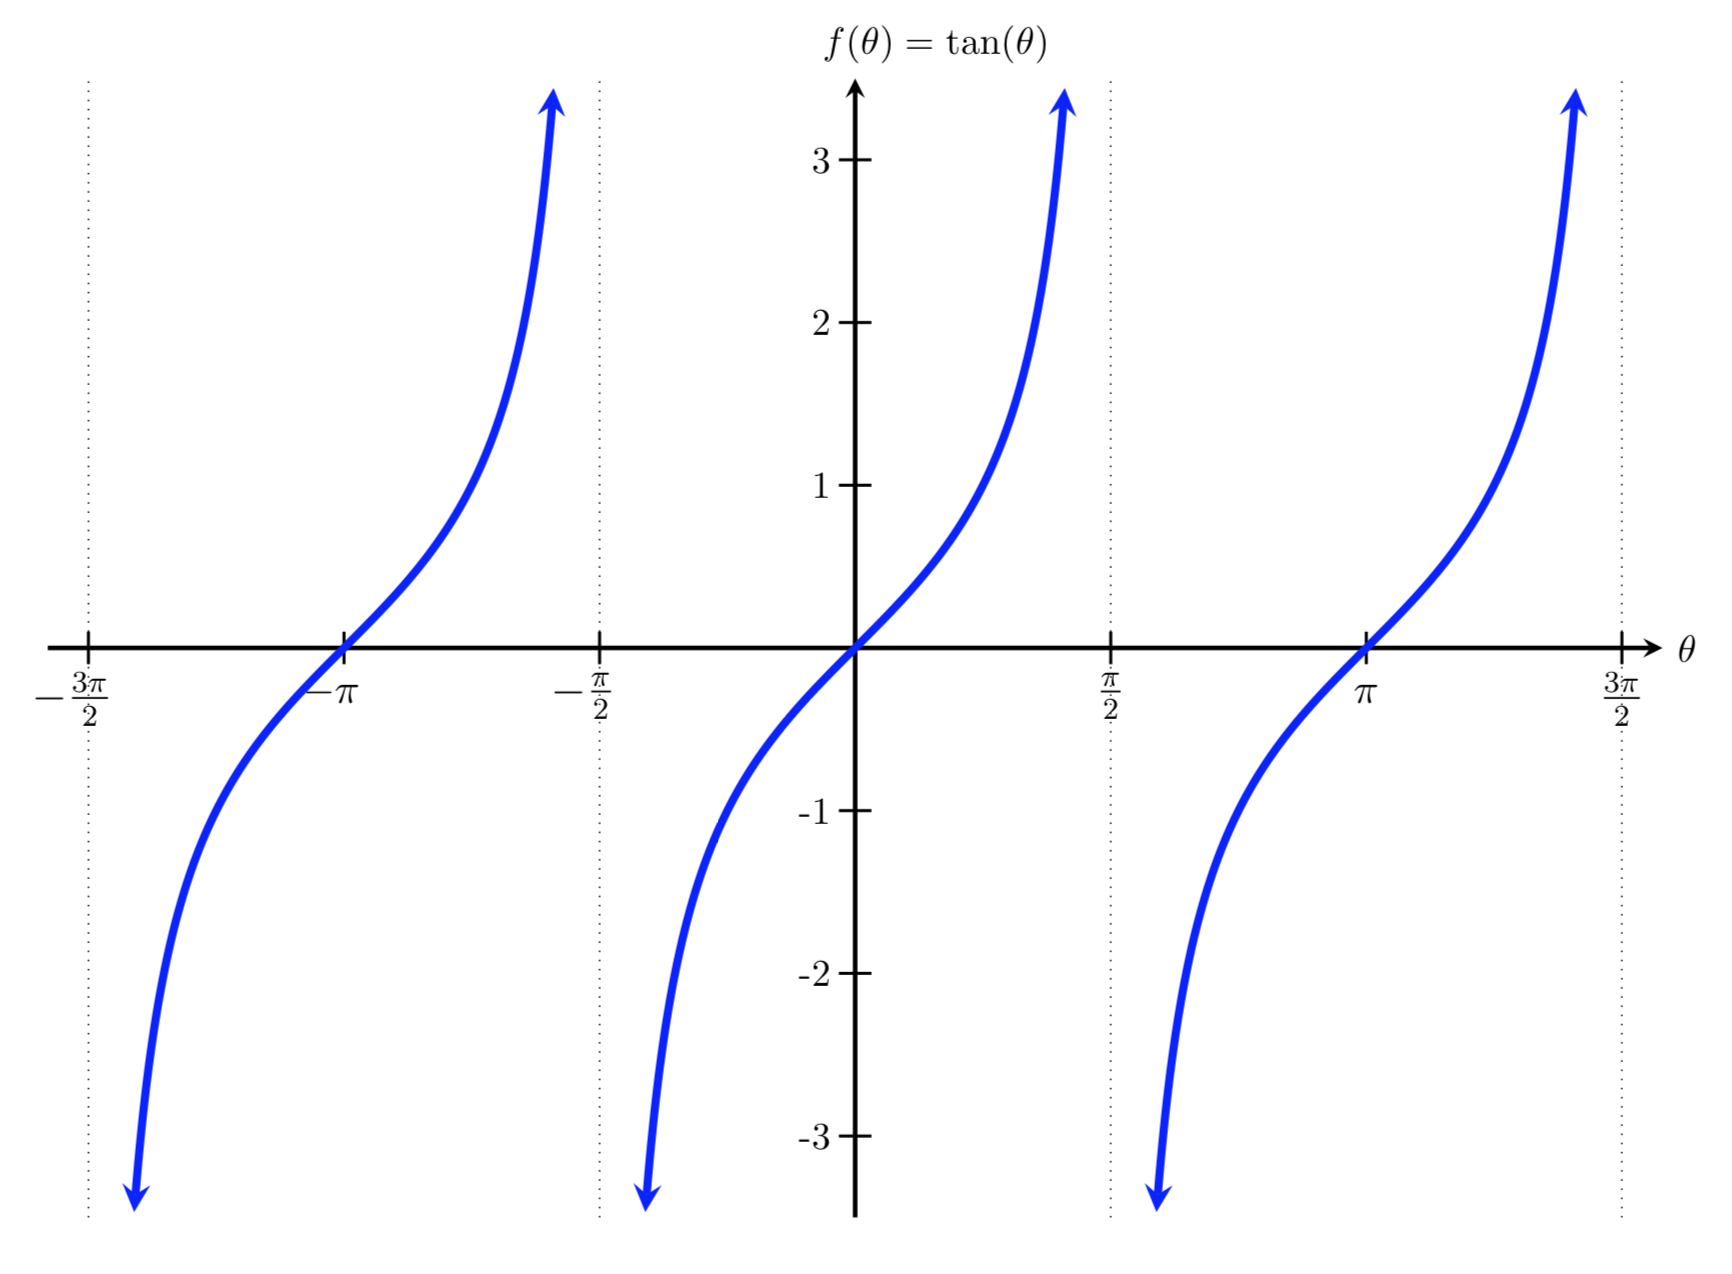
\includegraphics[width=\textwidth]{img/tangentgraph.png}
		\caption{Grafico della funzione $\tan$ (\href{https://mathbooks.unl.edu/PreCalculus/tangent-and-cofunctions.html}{fonte}).}
		\label{fig: esame 21 giugno 2023 - Gruppo A - 1 esercizio}
	\end{figure}
	\begin{equation*}
		-\dfrac{\pi}{2} < 3x^{2} - 12 < \dfrac{\pi}{2}
	\end{equation*}
	Adesso il ragionamento da fare per capire l'intervallo massimale non è banale. Inizialmente, magari presi dalla furia in sede d'esame, si potrebbe cadere nella tentazione di procedere immediatamente con l'esplicitazione della $x$:
	\begin{equation*}
		\begin{array}{rcl}
			3x^{2} - 12 &<& \dfrac{\pi}{2} \\ [1em]
			3x^{2} &<& \dfrac{\pi}{2} + 12 \\ [1em]
			x^{2} &<& \dfrac{\frac{\pi}{2}}{3} + 4 \\ [1em]
			x^{2} &<& \dfrac{\pi}{6} + 4 \\ [1em]
			x &<& \sqrt{\dfrac{\pi}{6} + 4}
		\end{array}
	\end{equation*}
	E a specchio anche l'altra parte (non si riportano i calcoli perché basta cambiare il segno...). Lo studente potrebbe erroneamente concludere dicendo che questo è l'intervallo massimale:
	\begin{equation*}
		\sqrt{- \dfrac{\pi}{6} + 4} < x < \sqrt{\dfrac{\pi}{6} + 4}
	\end{equation*}
	E in parte è vero, perché nei pressi di $x = 2$, dove l'equazione $3x^{2}-12$ si annulla, la precedente disuguaglianza è sensata. Ma \emph{attenzione} all'argomento della funzione $\tan$! L'equazione $3x^{2} - 12$ si annulla con i valori di $x = \pm 2$. Questo significa che vicino ai valori in cui si annulla, la $x$ potrebbe avere dei valori che interessano le condizioni dell'intervallo massimale che si sta prendendo in considerazione.\newline

	\noindent
	Nel dettaglio, con $x = 2$ la seguente disuguaglianza è sensata:
	\begin{equation*}
		\sqrt{- \dfrac{\pi}{6} + 4} < x < \sqrt{\dfrac{\pi}{6} + 4}
	\end{equation*}
	Per convincersi di ciò, si prenda come esempio $x = 2.1$, la disuguaglianza è vera:
	\begin{equation*}
		1.8645\cdots < 2.1 < 2.1268\cdots
	\end{equation*}
	Con $x = -2$ non è più sensata, poiché prendendo come valore $x = -2.1$ e sostituendola nell'intervallo trovato inizialmente:
	\begin{gather*}
		-\dfrac{\pi}{2} < 3\left(-2.1\right)^{2} - 12 < \dfrac{\pi}{2} \\ \\
		-1.57\cdots < 1.23 < 1.57 \hspace{.5em}
	\end{gather*}
	La disuguaglianza è vera, mentre con quella trovata esplicitando la $x$ no:
	\begin{equation*}
		1.8645\cdots < -2.1 < 2.1268\cdots
	\end{equation*}
	Per renderla vera, basta semplicemente affermare che l'intervallo massimale dipende dalla condizione iniziale:
	\begin{equation*}
		-\sqrt{\dfrac{\pi}{6} + 4} < x < -\sqrt{- \dfrac{\pi}{6} + 4} \hspace{1em} \lor \hspace{1em}
		\sqrt{- \dfrac{\pi}{6} + 4} < x < \sqrt{\dfrac{\pi}{6} + 4}
	\end{equation*}
	Si riportano qui i grafici della funzione $3x^{2} - 12$ e dell'intervallo massimale. Ed è interessare notare come il \dquotes{buco} tra i due intervalli sia causato dalla funzione che con quei valori di $x$ decresce a tal punto da non rispettare più la disuguaglianza.
	\begin{figure}[!htp]
		\centering
		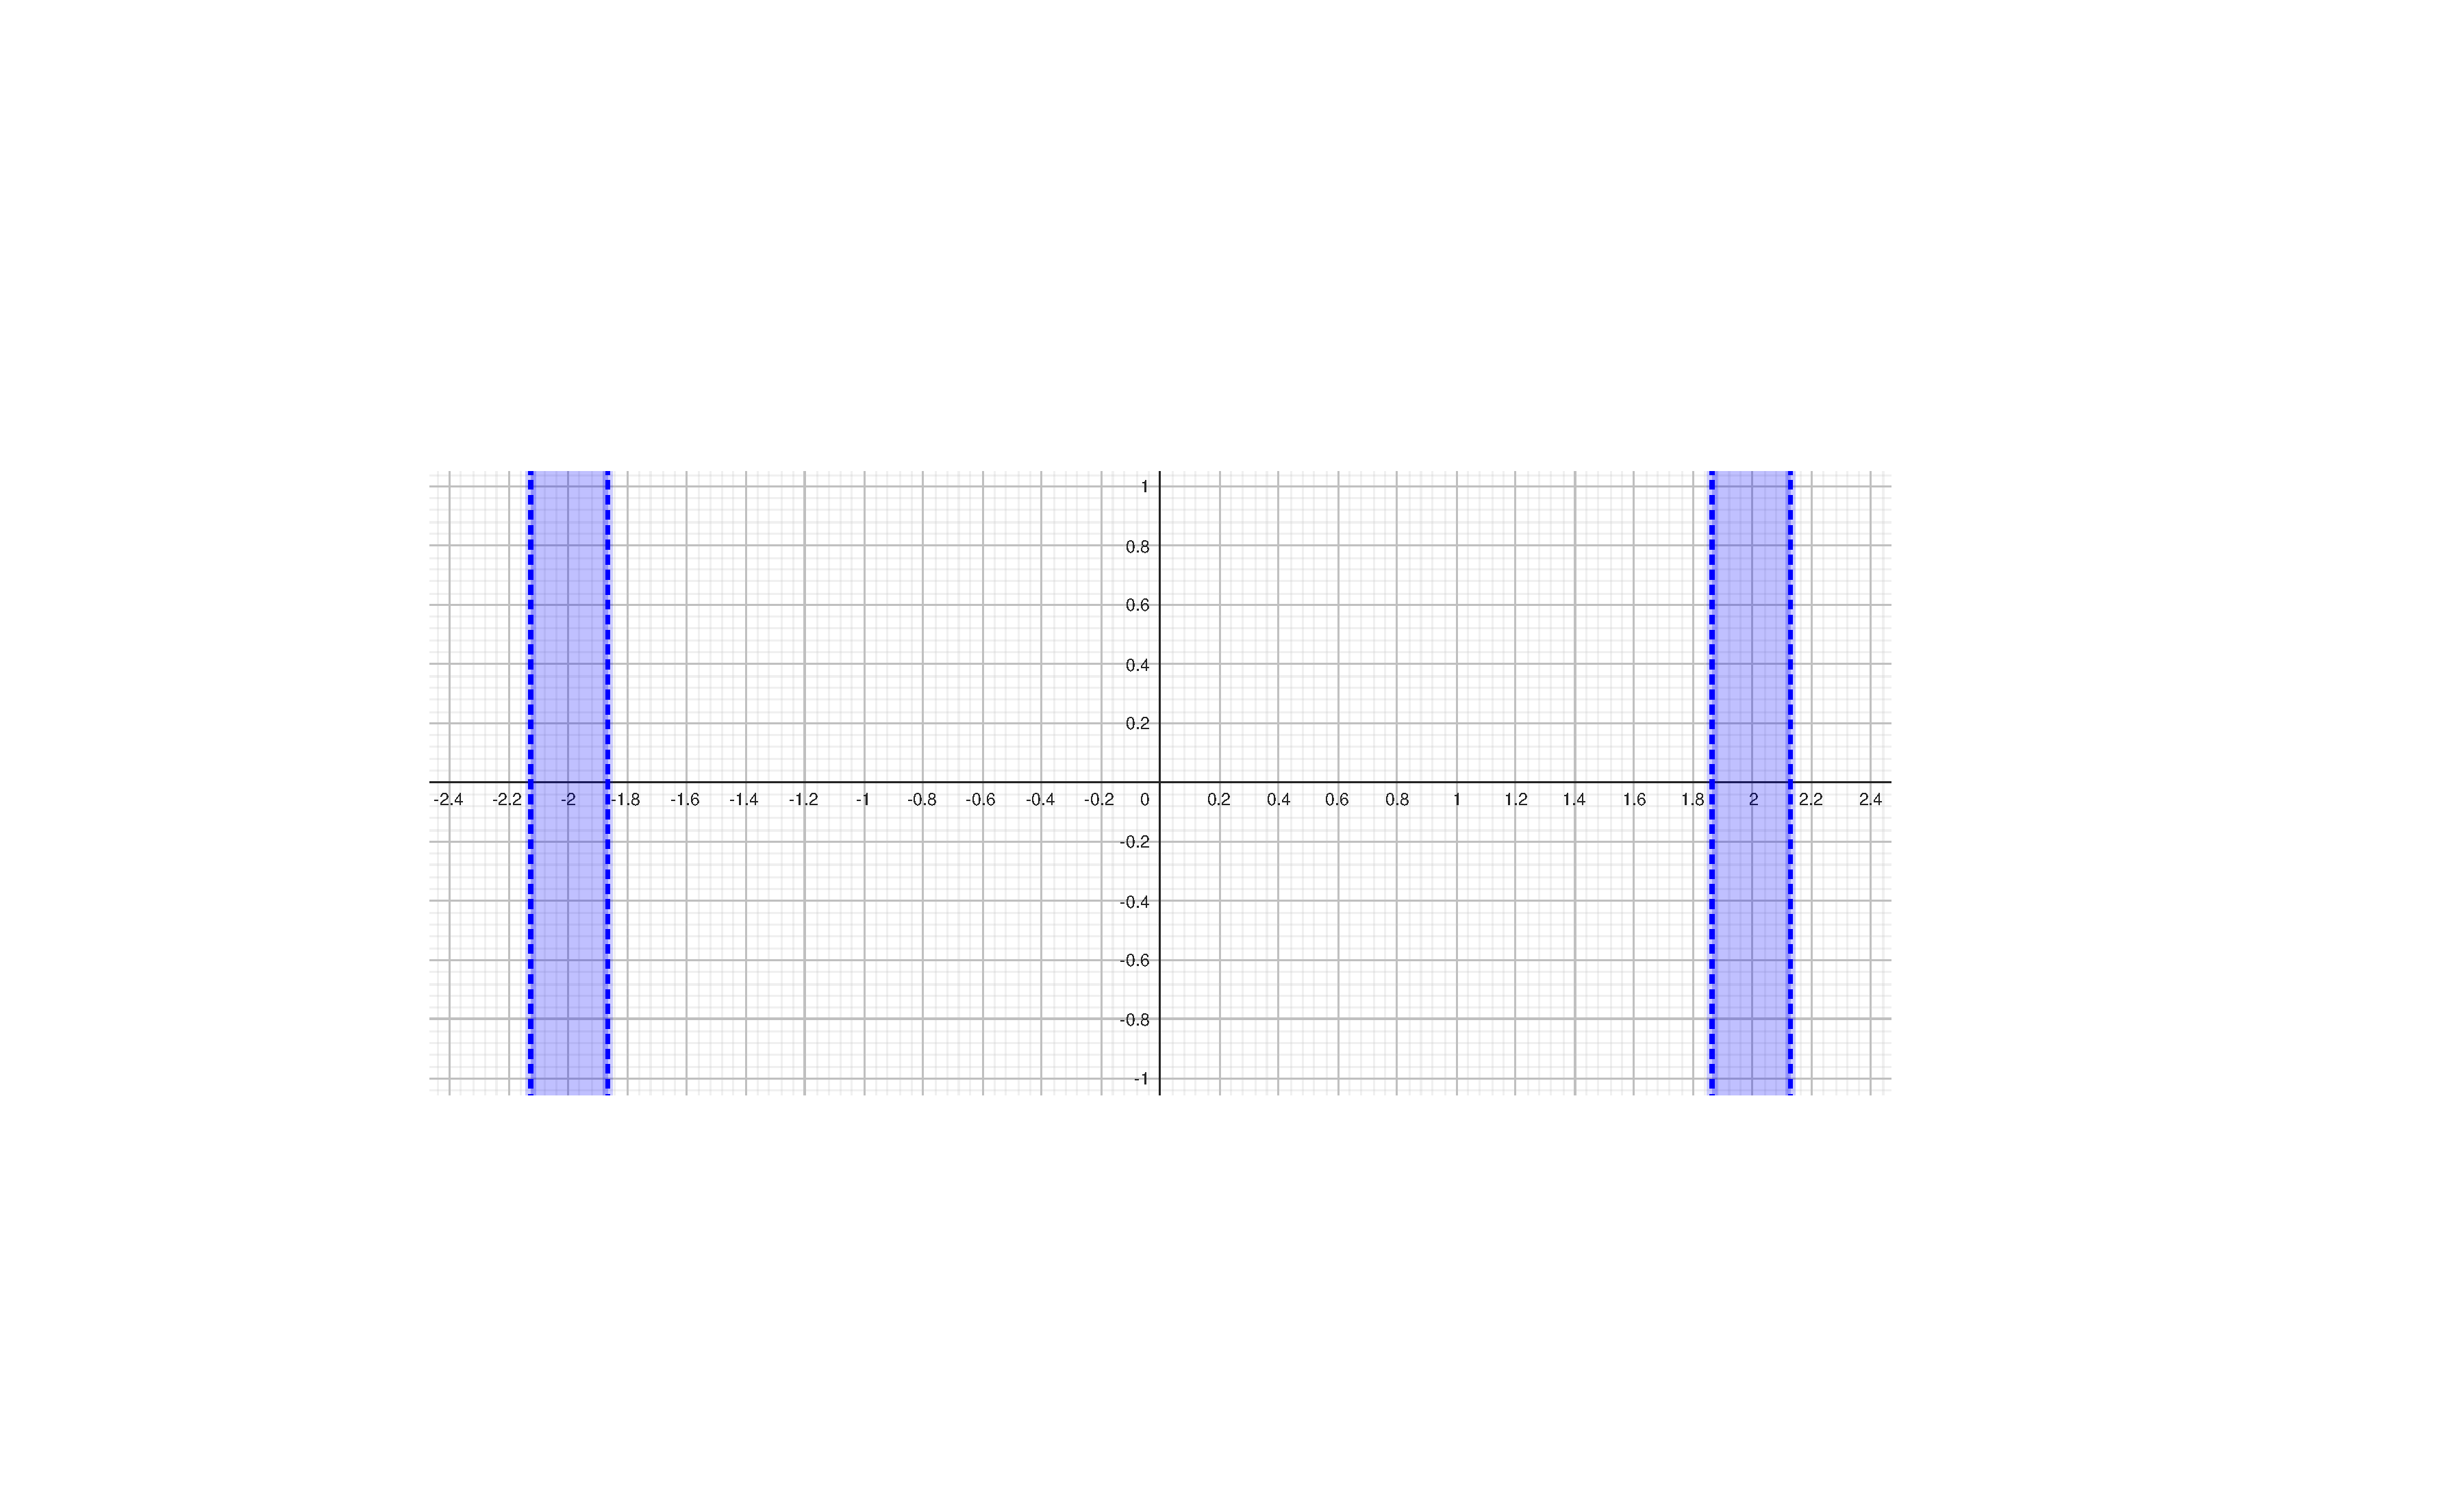
\includegraphics[width=\textwidth]{img/exercise/2023-06-21-A-ex1_2.pdf}
		\caption{Grafico dell'intervallo massimale.}
	\end{figure}\newpage

	\begin{figure}[!htp]
		\centering
		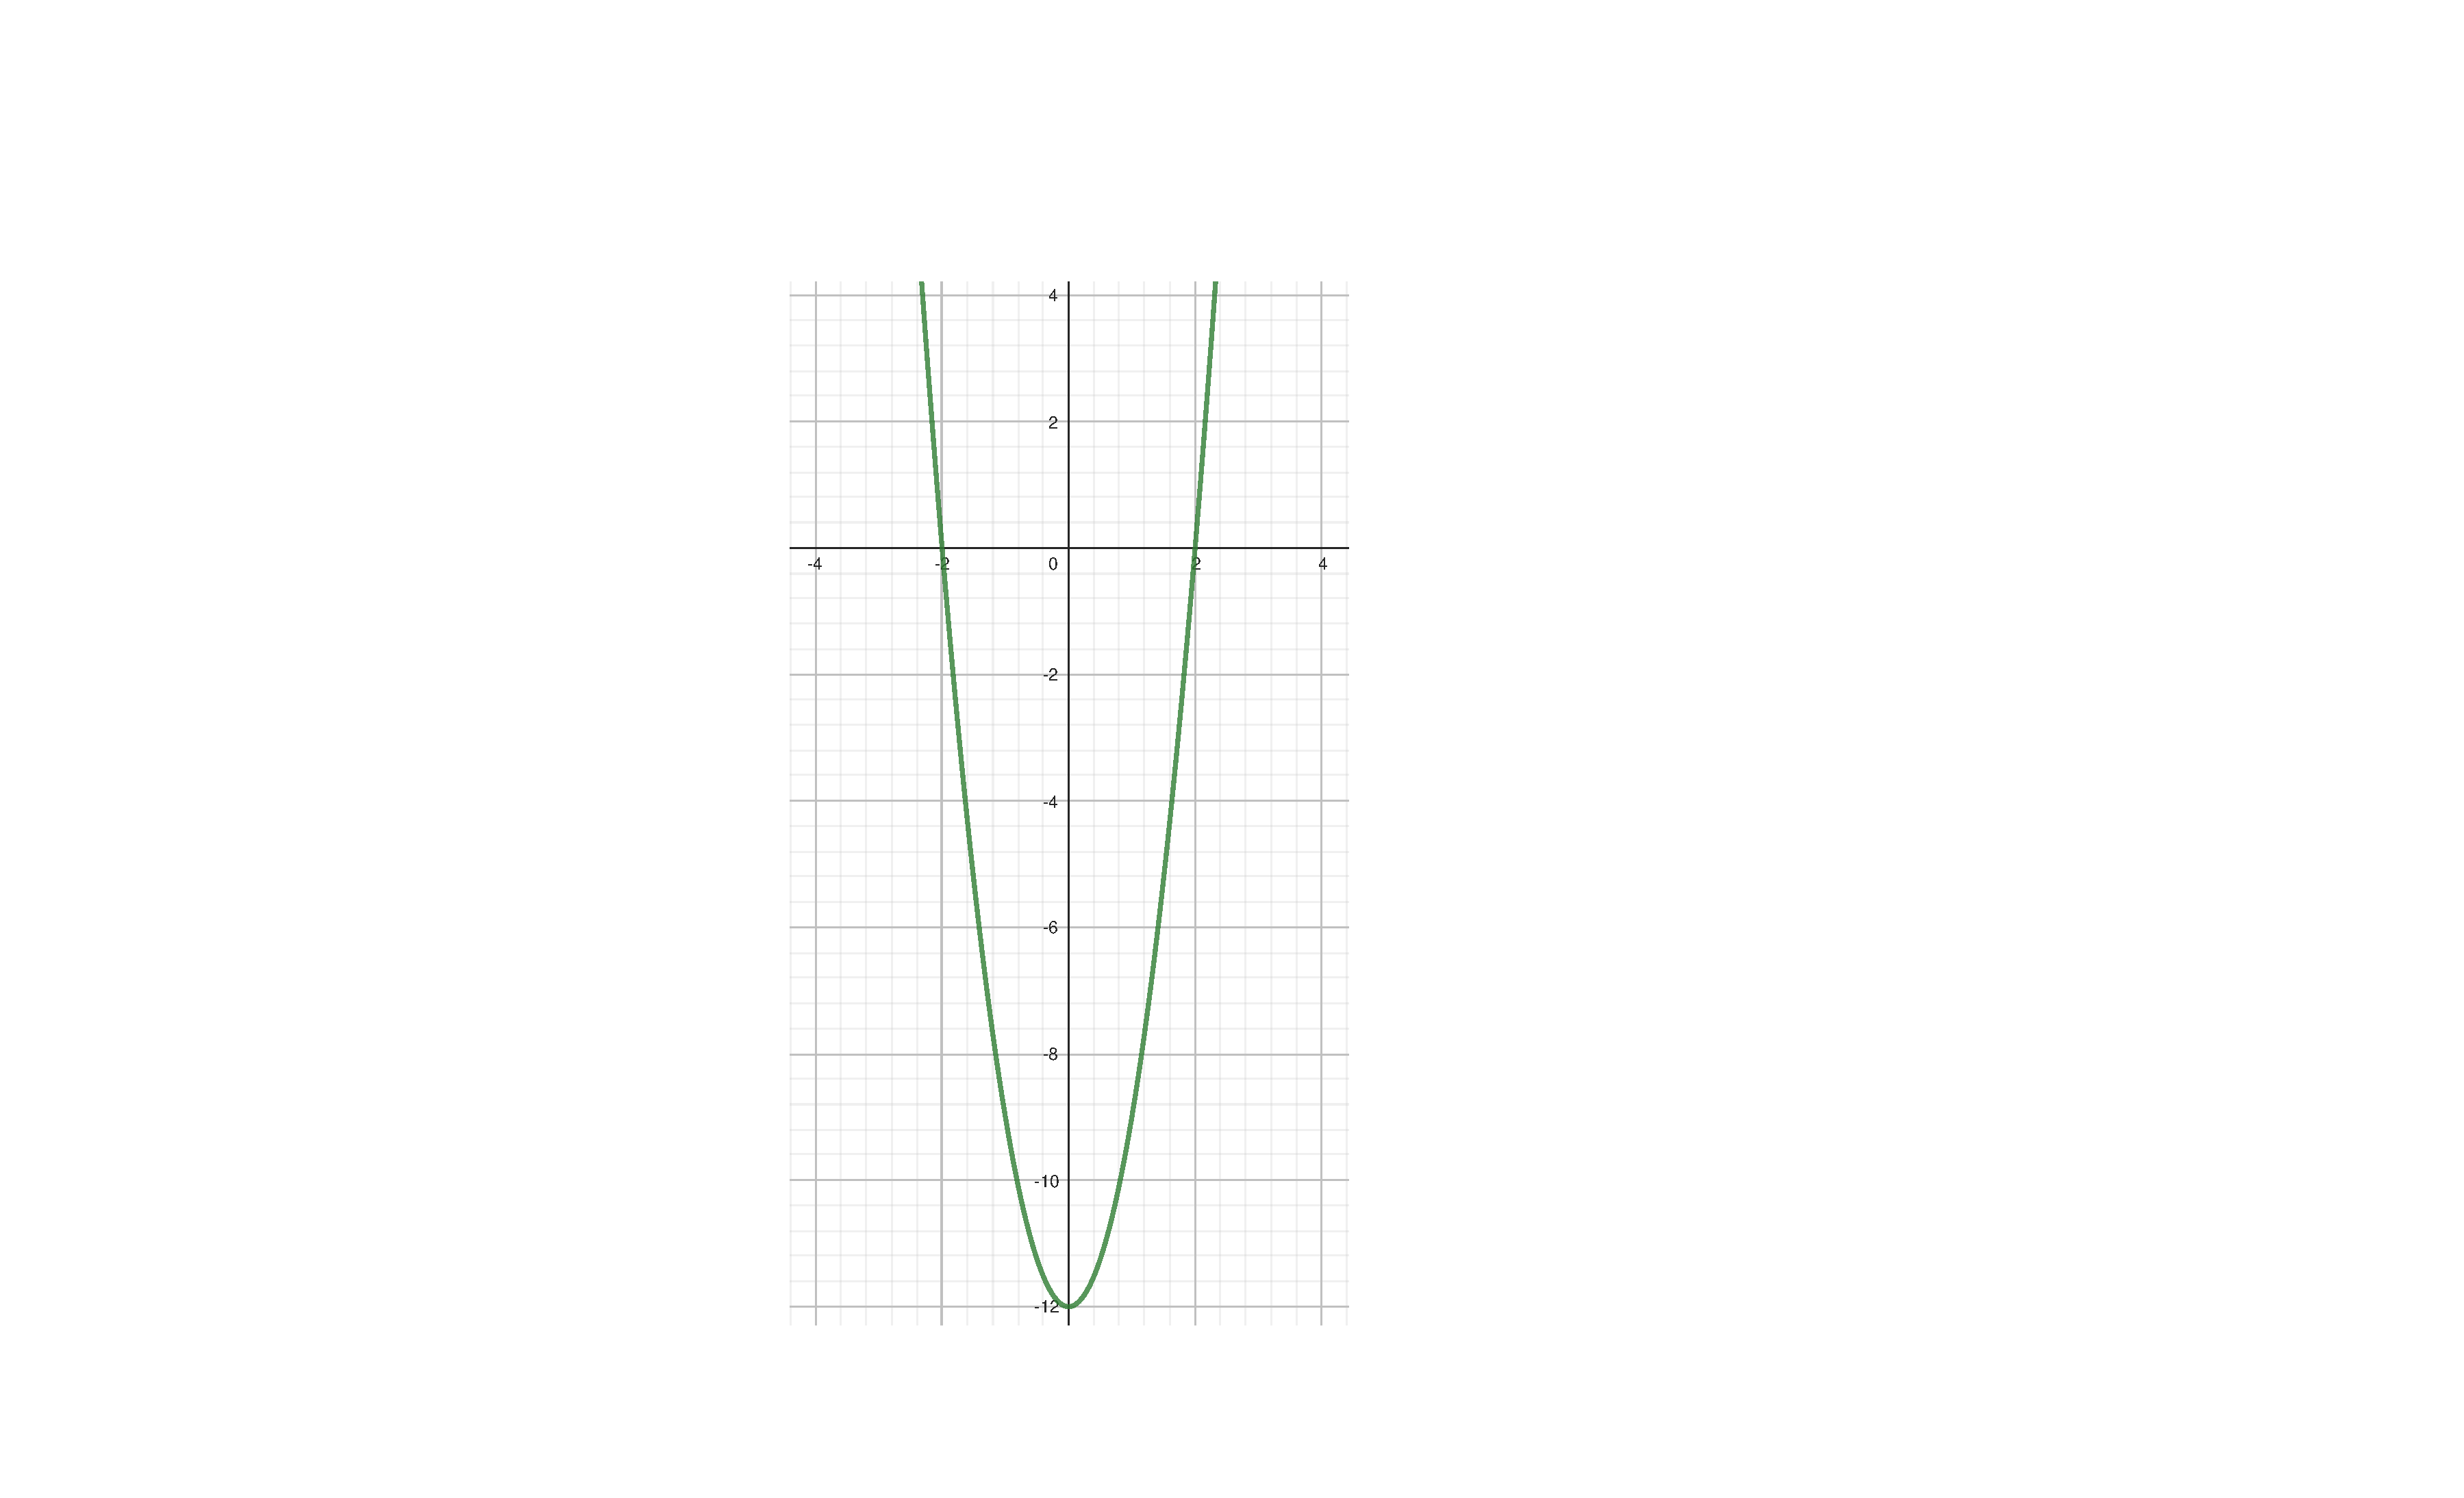
\includegraphics[width=.6\textwidth]{img/exercise/2023-06-21-A-ex1.pdf}
		\caption{Grafico della funzione $3x^{2}-12$.}
	\end{figure}

	\newpage

	\subsubsection{Metodo di somiglianza e problema di Cauchy}\label{subsubsection: metodo di somiglianza e problema di Cauchy}
	
	Work in progress...
	\newpage

	\subsubsection{Casi particolari}\label{subsubsection: casi particolari equazioni differenziali}

	\begin{flushleft}
		\example{\underline{E se non posso applicare le variabili separabili? Niente panico...}}
	\end{flushleft}

	\noindent
	Dato il seguente problema di Cauchy:
	\begin{equation*}
		\begin{cases}
			y' - \dfrac{y}{x} = 1 \\
			y\left(1\right) = 2
		\end{cases}
	\end{equation*}
	Non è possibile applicare direttamente la tecnica delle variabili separabili perché non è nella forma classica, sono necessarie prima alcune manipolazioni algebriche.\newline

	\noindent
	Si tenta di applicare la regola del prodotto (Reverse Product Rule) tra derivate ma all'inverso:
	\begin{equation*}
		\begin{array}{rcl}
			\dfrac{1}{x} \cdot \left(y' - \dfrac{y}{x}\right) &=& 1 \cdot \dfrac{1}{x} \\ [1em]
			%
			\left(\dfrac{1}{x} \cdot y'\right) + \left(-\dfrac{1}{x^{2}} \cdot y\right) &=& \dfrac{1}{x} \\ [1.5em]
			%
			&\downarrow & \text{ricordando l'integrale fondamentale: } \\
			&			& \displaystyle\int \dfrac{1}{x^{n}} \:\mathrm{d}x = - \dfrac{1}{\left(n-1\right) \cdot x^{n-1}} \hspace{1em} n \ne -1 \\ [2em]
			%
			&\downarrow& \displaystyle\int -\dfrac{1}{x^{2}} = \dfrac{1}{x} \\ [1em]
			%
			\left(\dfrac{1}{x} \cdot y'\right) + \left(\left(\dfrac{1}{x}\right)' \cdot y\right) &=& \dfrac{1}{x} \\ [1.5em]
			%
			&\downarrow & \text{ricordando la regola del prodotto tra derivate:} \\
			&			& \left[f\left(x\right) \cdot g\left(x\right)\right]' = f'\left(x\right) \cdot g\left(x\right) + f\left(x\right) \cdot g'\left(x\right) \\ [1.5em]
			%
			&\downarrow & \left(\dfrac{1}{x}\right)' \cdot y + \dfrac{1}{x} \cdot y' = \left[\dfrac{1}{x} \cdot y\right]' \\ [1.5em]
			%
			\left[\dfrac{1}{x} \cdot y\right]' &=& \dfrac{1}{x}
		\end{array}
	\end{equation*}
	Giunti a questo punto, non è possibile andare avanti cercando la disperata strada delle variabili separabili! Tuttavia, vi è un'opzione più semplice: risolverla come un'equazione lineare. Per cui, nella prossima pagina si presentano i calcoli.\newpage
	\begin{equation*}
		\begin{array}{rcl}
			\left[\dfrac{1}{x} \cdot y\right]' &=& \dfrac{1}{x} \\ [1.5em]
			%
			\displaystyle\int \left[\dfrac{1}{x} \cdot y\right]' \:\mathrm{d}x &=& \displaystyle\int \dfrac{1}{x} \:\mathrm{d}x \\ [1.5em]
			%
			\dfrac{1}{x} \cdot y &=& \ln\left(x\right) + c \\ [1em]
			%
			\cancel{x} \cdot \dfrac{1}{\cancel{x}} \cdot y &=& \left(\ln\left(x\right) + c\right) \cdot x  \\ [1em]
			%
			y &=& x\left(\ln\left(x\right) + c\right)
		\end{array}
	\end{equation*}
	Applicando la condizione iniziale $y\left(1\right) = 2$:
	\begin{equation*}
		\begin{array}{rcl}
			2 &=& 1 \cdot \left(\ln\left(1\right) + c\right) \\
			2 &=& c
		\end{array}
	\end{equation*}
	Quindi la soluzione finale del problema:
	\begin{equation*}
		y = x\left(\ln\left(x\right) + 2\right)
	\end{equation*}\newpage

	\begin{flushleft}
		\example{\underline{Altro esempio di risoluzione lineare}}
	\end{flushleft}
	Equazione differenziale:
	\begin{equation*}
		y' = e^{x} + 3y
	\end{equation*}
	La risolvo come un'equazione lineare. Cerco di sfruttare la regola del prodotto tra derivate:
	\begin{equation*}
		\left[f\left(x\right) \cdot g\left(x\right)\right]' = f'\left(x\right) \cdot g\left(x\right) + f\left(x\right) \cdot g'\left(x\right)
	\end{equation*}
	\begin{gather*}
		\begin{array}{rcl}
			y' &=& e^{x} + 3y \\ [.3em]
			y' - 3y &=& e^{x} \\ [1em]
			&\downarrow& \text{utilizzo l'esponenziale per cercare una forma accettabile} \\ [.3em]
			&& \displaystyle e^{\int -3 \:\mathrm{d}x} = e^{-3x} \\ [1em]
			e^{-3x} \cdot \left(y' - 3y\right) &=& e^{-3x} \cdot e^{x} \\ [.3em]
			\left(e^{-3x}\right)y' + \left(-3e^{-3x}\right)y &=& e^{-2x} \\ [1em]
			&\downarrow& \text{ora è possibile applicare la regola del prodotto tra derivate} \\ [.3em]
			&& \left(-3e^{-3x}\right)y + \left(e^{-3x}\right)y' = y' \cdot y + y \cdot y' = (e^{-3x} \cdot y)' \\ [1em]
			(e^{-3x} \cdot y)' &=& e^{-2x} \\ [1em]
			&\downarrow& \text{integrando ambo i lati} \\ [1em]
			\displaystyle\int(e^{-3x} \cdot y)' \:\mathrm{d}x &=& \displaystyle\int e^{-2x} \:\mathrm{d}x \\ [1em]
			e^{-3x} \cdot y &=& - \dfrac{1}{2} \cdot e^{-2x} + c \\ [1em]
			y &=& -\dfrac{1}{2} \cdot \dfrac{e^{-2x}}{e^{-3x}} + c \cdot \dfrac{1}{e^{-3x}} \\ [1em]
			y &=& -\dfrac{1}{2} \cdot e^{x} + c \cdot e^{3x}
		\end{array}
	\end{gather*}
	\newpage

	\section{Spazi funzionali}\label{section: spazi funzionali}

	Gli spazi funzionali sono il secondo argomento trattato durante il corso di Analisi II. È un argomento importante dal punto di visto teorico poiché è ha stretto contatto con l'esercizio d'esame.

	\longline

	\subsection{Lo spazio $\mathbb{R}^{n}$}\label{subsection: lo spazio R^n}

	Lo spazio $\mathbb{R}^{n}$ viene identificato nel seguente modo:
	\begin{equation*}
		\mathbb{R}^{n} = \left\{x = \left(x_{1}, x_{2}, \cdots, x_{n}\right) \: : \: x_{i} \in \mathbb{R}, \: 1 \le i \le n\right\}
	\end{equation*}
	Per comodità, quando $n = 2, 3$, verrà utilizzata la notazione:
	\begin{equation*}
		\left(x,y\right) \in \mathbb{R}^{2} \hspace{2em}
		\left(x,y,z\right) \in \mathbb{R}^{3}
	\end{equation*}
	Lo spazio $\mathbb{R}^{n}$ è uno \textbf{spazio vettoriale normato}. Si approfondisce il significato di questi termini. Con \emph{spazio vettoriale} si intende che vi sono alcune operazioni definite:
	\begin{equation*}
		\begin{array}{rrcl}
			\text{Dato:} & x &=& \left(x_{1}, x_{2}, \cdots, x_{n}\right) \\ [.3em]
			\text{Dato:} & y &=& \left(y_{1}, y_{2}, \cdots, y_{n}\right) \\ [.3em]
			\text{Somma:} & x+y & = & \left(x_{1}+y_{1}, x_{2}+y_{2}, \cdots, x_{n}+y_{n}\right) \\ [.3em]
			\text{Prodotto per uno scalare:} & \alpha x &=& \left(\alpha x_{1}, \alpha x_{2}, \cdots, \alpha x_{n}\right) \hspace{1em} \alpha \in \mathbb{R} \\ [.3em]
			\text{Prodotto scalare:} & x \cdot y &=& \displaystyle\sum_{i=1}^{n} x_{i} \cdot y_{i}
		\end{array}
	\end{equation*}
	Invece, con \emph{normato} si intende che è possibile definire all'interno dello spazio $\mathbb{R}^{n}$ una \textbf{norma}, ovvero una funzione del tipo:
	\begin{equation*}
		\begin{array}{rcl}
			|| \cdot || : \mathbb{R}^{n} &\rightarrow& \mathbb{R} \\
			x &\mapsto& || x ||
		\end{array}
	\end{equation*}
	Che possiede le seguenti \underline{proprietà}:
	\begin{itemize}
		\item $|| x || \ge 0$ per ogni $x \in \mathbb{R}^{n}$; $||x|| = 0$ se e solo se il vettore $x$ è tutto nullo, cioè $x = \left(0, 0, \cdots, 0\right)$.
		
		In \dquotes{matematichese}:
		\begin{equation*}
			|| x || \ge 0, \hspace{1.5em} \forall x \in \mathbb{R}^{n}; \hspace{2em} ||x|| = 0 \iff x = \left(0, 0, \cdots, 0\right)
		\end{equation*}

		\item $||\lambda x|| = || \lambda || || x ||$, per ogni $x \in \mathbb{R}^{n}$ e per ogni $\lambda \in \mathbb{R}$.
		
		In \dquotes{matematichese}:
		\begin{equation*}
			||\lambda \cdot x|| = || \lambda || \cdot || x || \hspace{2em} x \in \mathbb{R}^{n}, \lambda \in \mathbb{R}
		\end{equation*}

		\item $|| x + y || \le ||x|| + ||y||$, per ogni $x$ e $y$ appartenente a $\mathbb{R}^{n}$.
		
		In \dquotes{matematichese}:
		\begin{equation*}
			||x + y|| = ||x|| + ||y|| \hspace{2em} x,y \in \mathbb{R}^{n}
		\end{equation*}
	\end{itemize}
	Nella pratica, una $p$-esima norma in $\mathbb{R}^{n}$ è rappresentata come:
	\begin{equation}\label{eq: norma}
		\displaystyle \left|\left| x \right|\right|_{p} = \left(\sum_{i=1}^{n} \left|x_{i}\right|^{p}\right)^{\frac{1}{p}} = \sqrt[p]{\sum_{i=1}^{n} \left|x_{i}\right|^{p}}
	\end{equation}
	\begin{figure}[!htp]
		\centering
		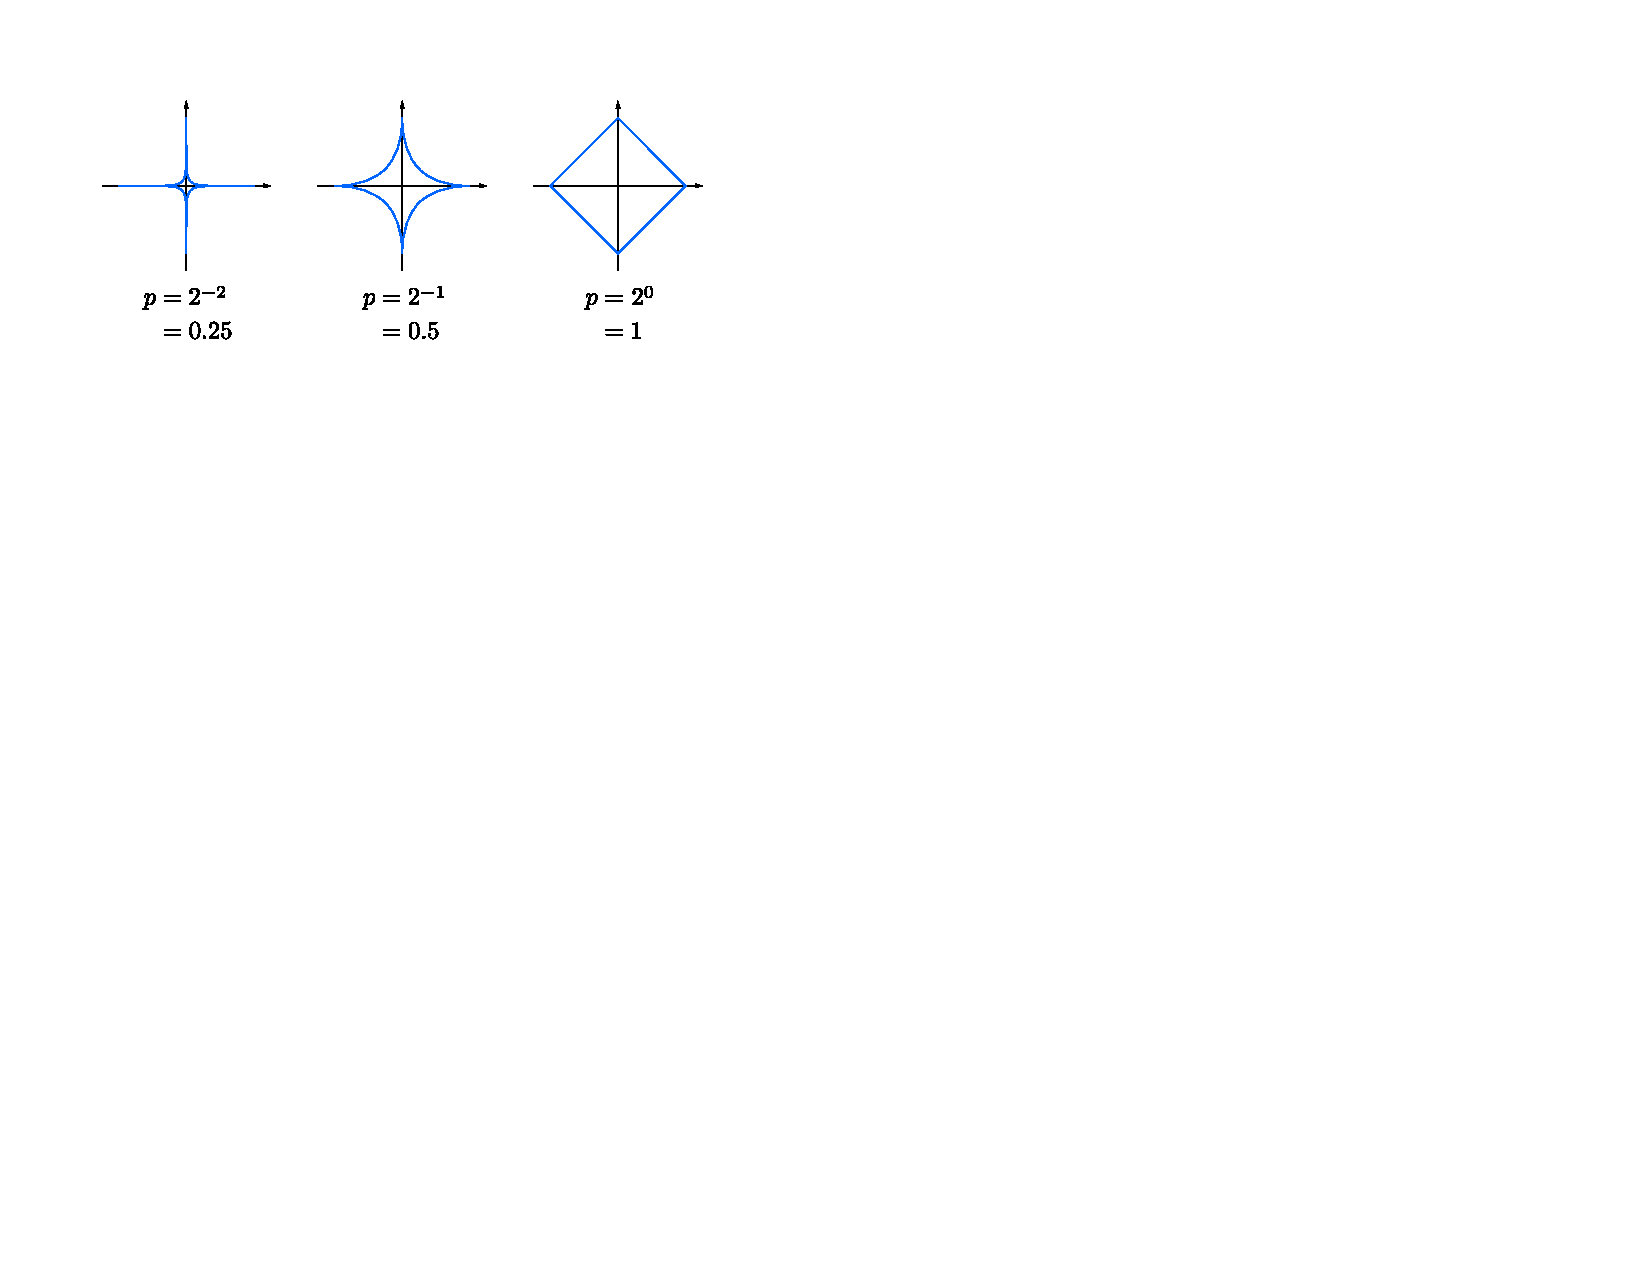
\includegraphics[width=.8\textwidth]{img/rappresentazione_n=2_1.pdf}
		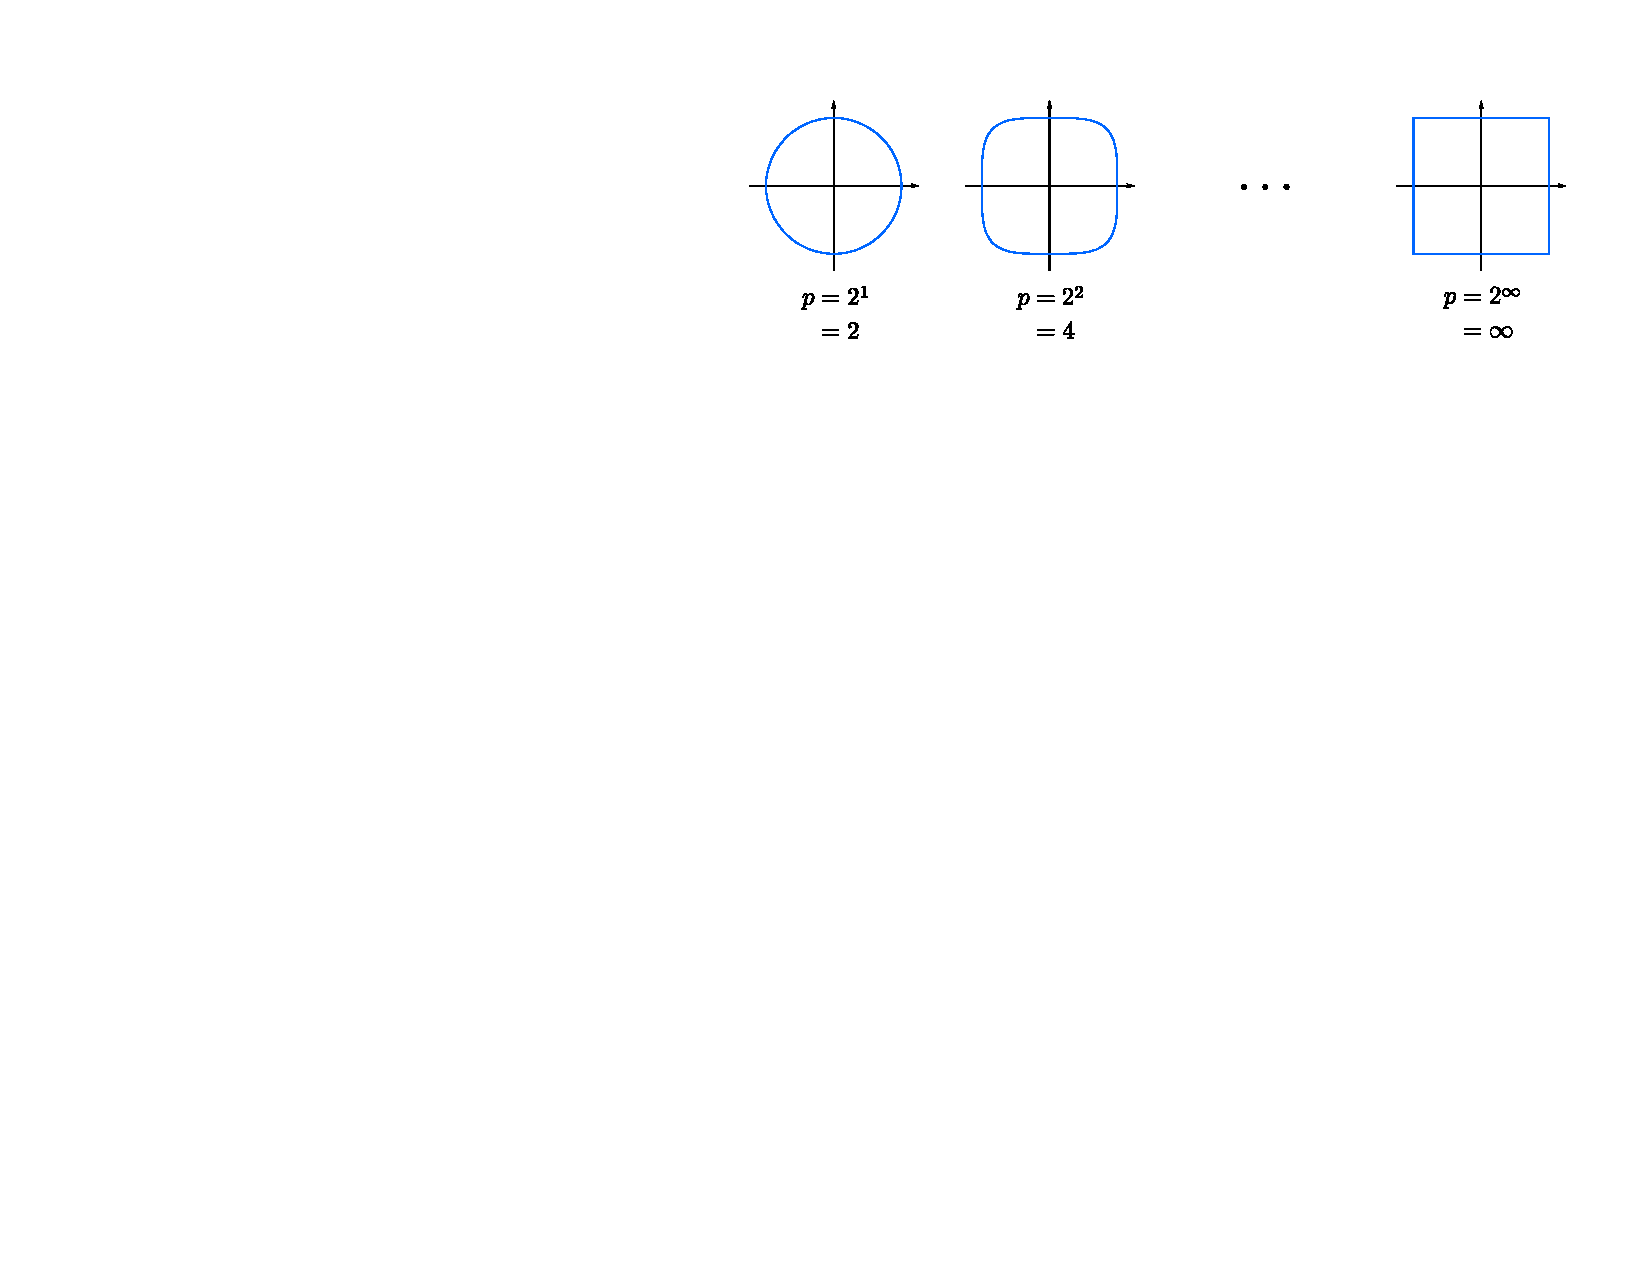
\includegraphics[width=.9\textwidth]{img/rappresentazione_n=2_2.pdf}
		\caption{Alcune rappresentazioni di norme in due dimensioni ($\mathbb{R}^{2}$).}
		\label{fig: alcune rappresentazioni di norme in due dimensioni}
	\end{figure}

	\noindent
	Il concetto di norma consente di mettere a fuoco che cosa si intende per \textbf{\dquotes{lunghezza} di un vettore} o \textbf{\dquotes{distanza} di un punto dall'origine}. \example{Per esempio}, nella seguente figura, ipotizzando che sia possibile muoversi solo lungo le linee del reticolo, la \dquotes{distanza} tra i due punti è $7$ e non $\sqrt{29}$ (teorema di pitagora, $\sqrt{5^{2} + 2^{2}}$). Questo perché banalmente viene sommata l'ascissa con l'ordinata, ovvero $5$ ($x$) e $2$ ($y$).
	\begin{equation*}
		\left(x_{1},x_{2}\right) = \left(5,2\right) \longrightarrow \left|\left| x \right|\right|_{1} = \left(\sum_{i=1}^{2} \left| x_{i} \right|^{1}\right)^{\frac{1}{1}} = 5 + 2 = 7
	\end{equation*}
	\vspace{-2em}
	\begin{figure}[!htp]
		\centering
		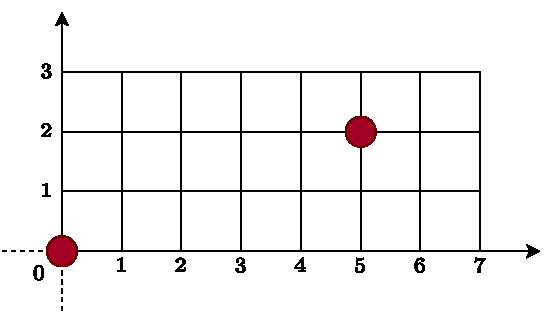
\includegraphics[width=.6\textwidth]{img/norma.pdf}
		\caption{Esempio di norma.}
		\label{fig: esempio di norma}
	\end{figure}\newpage

	\noindent
	E tra tutte le norme esistenti, la \textbf{norma euclidea} è la più interessante:
	\begin{equation}\label{eq: norma euclidea}
		\left|\left| x \right|\right|_{2} = \sqrt{x \cdot x} = \sqrt{\displaystyle \sum_{i=1}^{n} x^{2}_{i}}
	\end{equation}
	Un'altra disuguaglianza interessante è la \textbf{disuguaglianza di Cauchy-Schwarz}. Per ogni $x,y \in \mathbb{R}^{n}$ si ha:
	\begin{equation}\label{eq: disuguaglianza di Cauchy-Schwarz}
		|x \cdot y| \le ||x|| \cdot ||y||
	\end{equation}
	Il motivo per cui sono stati introdotti questi concetti è evidente con il prossimo paragrafo.\newpage

	\subsection{Spazio metrico e distanza (euclidea)}\label{subsection: spazio metrico e distanza}

	\begin{boxdef}
		Un insieme $X$ si dice \textbf{spazio metrico} se è definita un'applicazione, chiamata \textbf{distanza} o \textbf{metrica}
		\begin{equation*}
			d: X \times X \rightarrow \mathbb{R}
		\end{equation*}
		Tale che per ogni $x,y,z \in X$ valgono le seguenti proprietà:
		\begin{itemize}
			\item $d\left(x,y\right) \ge 0$; \hspace{2em} $d\left(x,y\right) = 0 \iff x = y$
			
			\item $d\left(x,y\right) = d\left(y,x\right)$
			
			\item $d\left(x,y\right) \le d\left(x,z\right) + d\left(z,y\right)$
		\end{itemize}
	\end{boxdef}

	\noindent
	Si sottolinea che uno spazio metrico è una coppia insieme-distanza o metrica, ovverosia $d\left(X, d\right)$. Questo perché su uno stesso insieme $X$ potrebbero definirsi più metriche diverse ($d_{1}, d_{2}, d_{3}, \cdots$).\newline

	\noindent
	Particolarmente interessante è la \textbf{distanza euclidea} che viene indotta dalla norma euclidea (equazione \ref{eq: norma euclidea}):
	\begin{equation}\label{eq: distanza euclidea}
		d\left(x,y\right) = ||x-y|| = \sqrt{\displaystyle\sum_{i=1}^{n}\left(x_{i} - y_{i}\right)^{2}}
	\end{equation}
	Un \example{esempio} chiarificatore può essere la distanza euclidea tra i due punti presenti nella seguente figura:
	\begin{figure}[!htp]
		\centering
		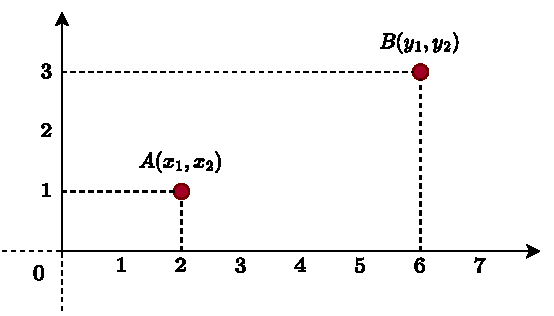
\includegraphics[width=.8\textwidth]{img/distanza_euclidea.pdf}
	\end{figure}
	
	\noindent
	La distanza dunque viene calcolata come (ricordando che $n = 2$ intuibile dal pedice massimo delle variabili nel grafico):
	\begin{equation*}
		d\left(A, B\right) = \sqrt{\left(x_{1}-y_{1}\right)^{2} + \left(x_{2}-y_{2}\right)^{2}}
	\end{equation*}
	Nonostante le notazioni classiche utilizzino $\left(x,y\right)$ per rappresentare i punti, in questo caso è necessario utilizzare la notazione in figura poiché in caso di dimensioni più grandi (quindi di $n$ maggiori) risulta poco efficiente.

	\subsection{Topologia in $\mathbb{R}^{n}$}\label{subsection: topologia in R^n}

	\subsubsection{Palla aperta}\label{subsubsection: palla aperta}

	\begin{boxdef}
		Se $\left(X,d\right)$ è uno spazio metrico e $x \in X$, si chiama \textbf{intorno sferico di $x$} (o \textbf{palla di centro $x$}) di raggio $r$ l'insieme:
		\begin{equation}\label{eq: palla di centro x (formale)}
			B\left(x,r\right) = \left\{y \in X \: : \: d\left(x,y\right) < r\right\}
		\end{equation}
	\end{boxdef}

	\noindent
	È possibile esprimere una \textbf{palla aperta} di centro $\overline{x}$ e raggio $r>0$ più chiaramente come:
	\begin{equation}\label{eq: palla di centro x (informale)}
		B_{r}\left(\overline{x}\right) = \left\{x \in \mathbb{R}^{n} \: : \: || x - \overline{x} || < r\right\}
	\end{equation}
	Per \example{esempio}:
	\begin{itemize}
		\item Una palla aperta di centro $x$ con $\boldsymbol{n=1}$ è:
		\begin{equation*}
			B_{r}\left(\overline{x}\right) = \left\{x \in \mathbb{R} \: : \: |x-\overline{x}| < r\right\} = \left\{x\in\mathbb{R} \: : \: \overline{x}-r < x < \overline{x}+r\right\}
		\end{equation*}
		Che graficamente è:
		\begin{figure}[!htp]
			\centering
			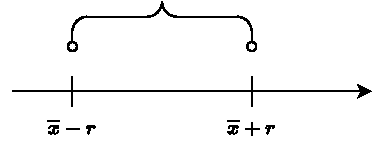
\includegraphics[width=.5\textwidth]{img/palla_aperta_n=1.pdf}
		\end{figure}

		\item Una palla aperta di centro $x$ con $\boldsymbol{n=2}$ (con $\left(x_{0},y_{0}\right)$ si indica il centro, $x_{0}, y_{0} \in \mathbb{R}$) è:
		\begin{equation*}
			\begin{array}{rcl}
				B_{r}\left(c\right) &=& \left\{\left(x,y\right) \in \mathbb{R}^{2} \: : \: \sqrt{\left(x-x_{0}\right)^{2} + \left(y-y_{0}\right)^{2}} < r \right\} \\ [1em]
				&=& \left\{\left(x,y\right)\in\mathbb{R}^{2} \: : \: \left(x-x_{0}\right)^{2} + \left(y-y_{0}\right)^{2} < r^{2}\right\}
			\end{array}
		\end{equation*}
		Che graficamente è:
		\begin{figure}[!htp]
			\centering
			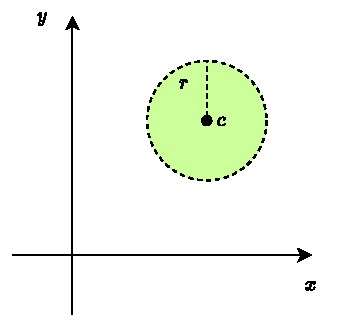
\includegraphics[width=.4\textwidth]{img/palla_aperta_n=2.pdf}
		\end{figure}\newpage

		\item Una palla aperta di centro $x$ con $\boldsymbol{n=3}$ (con $\left(x_{0}, y_{0}, z_{0}\right)$ si indica il centro, $x_{0}, y_{0}, z_{0} \in \mathbb{R}$) è:
		\begin{equation*}
			\begin{array}{rcl}
				B_{r}\left(c\right) &=& \left\{\left(x,y,z\right) \in \mathbb{R}^{3} \: : \: \sqrt{\left(x-x_{0}\right)^{2} + \left(y-y_{0}\right)^{2} + \left(z-z_{0}\right)^{2}} < r \right\} \\ [1em]
				%
				&=& \left\{\left(x,y\right)\in\mathbb{R}^{2} \: : \: \left(x-x_{0}\right)^{2} + \left(y-y_{0}\right)^{2} + \left(z-z_{0}\right)^{2} < r^{2}\right\}
			\end{array}
		\end{equation*}
		Che graficamente è:
		\begin{figure}[!htp]
			\centering
			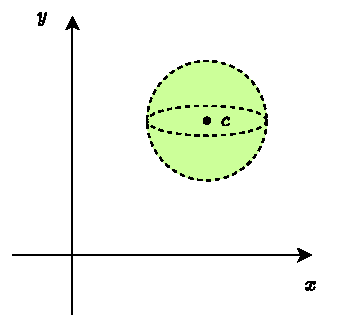
\includegraphics[width=.45\textwidth]{img/palla_aperta_n=3.pdf}
		\end{figure}
	\end{itemize}
	Si presenta anche un esercizio. 
	
	\begin{flushleft}
		\example{\underline{Esercizio}}
	\end{flushleft}

	\noindent
	Rappresentare graficamente:
	\begin{equation*}
		\left\{x \in \mathbb{R}^{2} \: : \: ||x|| < 1\right\}
	\end{equation*}
	Dalla definizione di palla aperta (equazione \ref{eq: palla di centro x (formale)}, ma più evidente nell'equazione informale \ref{eq: palla di centro x (informale)}) si ricava che il raggio è uguale a $r = 1$. Inoltre, il termine $\overline{x}$, che rappresenta le coordinate del centro della palla, non è presente, dunque si deduce che sia uguale a zero ($||x - \overline{x}|| = ||x - 0|| = || x ||$).

	\noindent
	Dall'esempio in figura a pagina \pageref{fig: esempio di norma}, la norma, ovvero $|| x ||$, si rappresenta sommando le sue coordinate (come nell'equazione \ref{eq: norma}). Per cui, per rappresentare $||x|| < 1$, si deve affermare che:
	\begin{equation*}
		|| x || < 1 \longrightarrow |x_{1}| + |x_{2}| < 1
	\end{equation*}
	Con $x_{1}$ che rappresenta l'asse delle $x$ e $x_{2}$ che rappresenta l'asse delle $y$.\newline

	\noindent
	La rappresentazione grafica è possibile vederla chiaramente a pagina \pageref{fig: alcune rappresentazioni di norme in due dimensioni} in cui è possibile osservare alcune rappresentazioni di norma in due dimensioni.\newpage

	\subsubsection{Intorno di un punto}\label{subsubsection: intorno di un punto}

	L'\definition{intorno di un punto} $\overline{x}$ si definisce come:
	\begin{equation*}
		U \subseteq \mathbb{R}^{n}
	\end{equation*}
	Se esiste $r > 0$ (cioè un raggio maggiore di zero) tale per cui una palla aperta di centro $\overline{x}$ è contenuta in $U$:
	\begin{equation*}
		B_{r}\left(\overline{x}\right) \subseteq U
	\end{equation*}

	\begin{flushleft}
		\example{\underline{Esempio}}
	\end{flushleft}

	\begin{figure}[!htp]
		\centering
		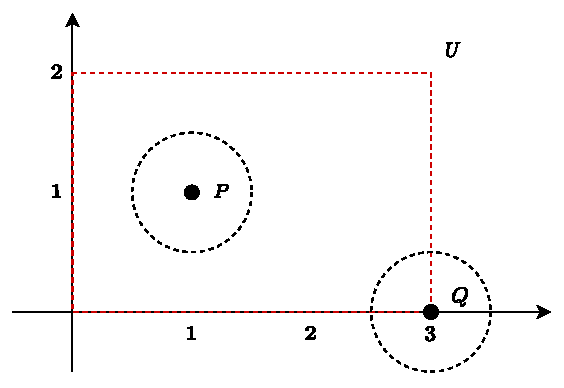
\includegraphics[width=.8\textwidth]{img/intorno_di_un_punto.pdf}
	\end{figure}

	\noindent
	Dato l'insieme:
	\begin{equation*}
		U = \left(0,3\right) \times \left(0,2\right)
	\end{equation*}
	Esso è un intorno di $P$ poiché $B_{\frac{1}{2}}\left(P\right) \subseteq U$. Al contempo, $U$ non è un intorno di $Q$ poiché non esiste un raggio appartenente a $\mathbb{R}^{+}$ tale che una palla con quel raggio sia contenuta dentro $U$:
	\begin{equation*}
		\nexists \: r \in \mathbb{R}^{+} \hspace{.5em} t.c. \hspace{.5em} B_{r}\left(Q\right) \subseteq U
	\end{equation*}
	Infatti con $\left(3+\dfrac{r}{2}, 0\right) \in B_{r}\left(Q\right)$ per ogni $r>0$, viene di conseguenza che $\left(3+\dfrac{r}{2}, 0\right) \notin U$.\newpage

	\subsubsection{Punti interni, esterni e di frontiera}\label{subsubsection: punti interni, esterni e di frontiera}

	\begin{figure}[!htp]
		\centering
		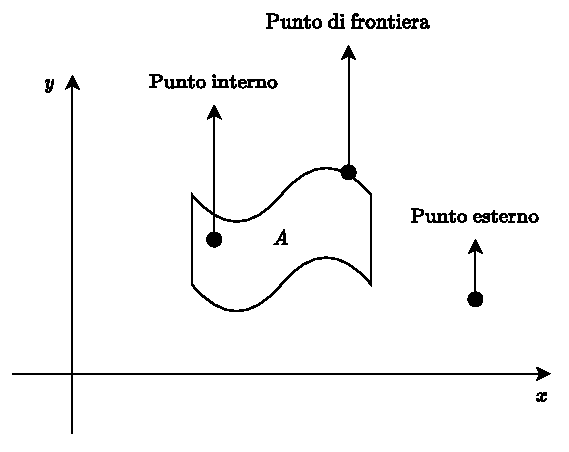
\includegraphics[width=.8\textwidth]{img/punto-interno_esterno_frontiera.pdf}
	\end{figure}

	\begin{itemize}
		\item Un punto $P$ è \definition{interno} ad $A$ se esiste un raggio $r>0$ tale che la sua palla sia contenuta in $A$.
		\begin{equation*}
			r > 0 \hspace{.5em} t.c. \hspace{.5em} B_{r}\left(P\right) \subseteq A \Longrightarrow P \text{ è interno ad } A 
		\end{equation*}
		L'\textbf{insieme} dei punti interni all'insieme $A$ è rappresentato con il simbolo $\mathring{A}$ o con la scritta $\mathrm{int}\left(A\right)$.

		\item Un punto $P$ è \definition{esterno} ad $A$ se è un punto interno a $\mathbb{R}^{n}$ ma non ad $A$:
		\begin{equation*}
			P \text{ interno a } \mathbb{R}^{n} \setminus A \Longrightarrow P \text{ esterno a } A
		\end{equation*}
		L'\textbf{insieme} dei punti esterni si indica con $\mathrm{ext}\left(A\right)$. E questo tipo di insieme viene chiamato anche \textbf{complementare} di $A$ in $\mathbb{R}^{n}$.

		\item Un punto $P$ è \definition{frontiera} di $A$ se non è né interno né esterno ad $A$. L'\textbf{insieme} dei punti di frontiera si indica con $\partial A$.
	\end{itemize}
	Infine, si esprime come \definition{chiusura} di $A$ ($\overline{A}$), l'unione tra l'insieme stesso e i punti di frontiera, ovvero:
	\begin{equation*}
		\overline{A} = A \cup \partial A
	\end{equation*}
	Per vedere alcuni esempi, andare alla fine del prossimo paragrafo.\newpage

	\subsubsection{Insiemi aperti, chiusi e limitati}\label{subsubsection: insiemi aperti, chiusi e limitati}

	\begin{itemize}
		\item Un insieme $A$ è \definition{aperto} se è intorno di ogni suo punto. 
		
		Quindi l'insieme è aperto \textbf{se e solo se} $A = \mathring{A}$, ovvero se l'\textbf{insieme è uguale all'insieme dei punti interni}.
		
		\item Un insieme è \definition{chiuso} se il suo complementare (insieme dei punti esterni) è aperto.
		
		Quindi l'insieme è chiuso \textbf{se e solo se} $A = \overline{A}$, ovvero se l'\textbf{insieme è uguale all'insieme dei punti esterni}.

		\item Un insieme $A \subseteq \mathbb{R}^{n}$ è \definition{limitato} se esiste un raggio maggiore di zero $r > 0$ tale che una palla nel punto zero con quel raggio contenga l'insieme $A$ ($A \subseteq B_{r}\left(0\right)$).
		
		In altre parole, l'\textbf{insieme} $A$ \textbf{è limitato se esiste un raggio maggiore di zero tale per cui la norma} $x$ (somma delle sue coordinate in parole poverissime) \textbf{è minore del raggio per ogni} $x$ \textbf{appartenente ad} $A$:
		\begin{equation*}
			\exists \: r > 0 \hspace{.5em} t.c. \hspace{.5em} ||x|| < r \: , \hspace{.5em} \forall x \in A \Longrightarrow A \text{ è limitato}
		\end{equation*}
	\end{itemize}
	Gli insiemi $\mathbb{R}^{n}$ e $\emptyset$ sono gli unici insiemi aperti e chiusi in $\mathbb{R}^{n}$.\newpage
	
	\begin{flushleft}
		\example{\underline{Esempio 1}}
	\end{flushleft}

	\noindent
	Dato l'insieme $A$:
	\begin{equation*}
		A = \left\{x \in \mathbb{R}^{2} \: : \: 2 \le ||x|| < 3 \right\}
	\end{equation*}
	La sua rappresentazione grafica:
	\begin{figure}[!htp]
		\centering
		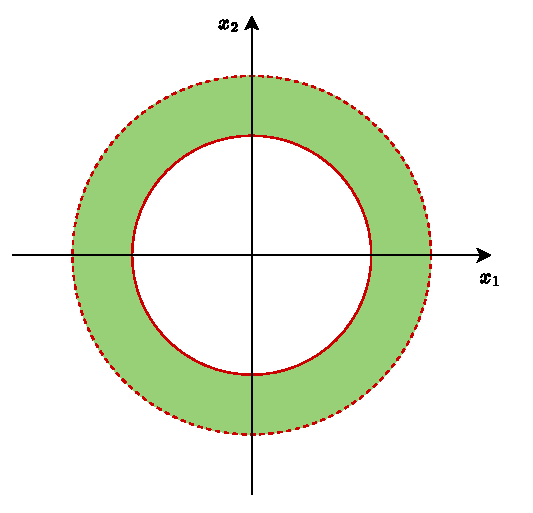
\includegraphics[width=.7\textwidth]{img/insiemi_aperti-chiusi-1.pdf}
	\end{figure}

	\noindent
	Si calcolano i vari insiemi per capire se è aperto, chiuso, limitato (e di conseguenza quali sono i punti interni, esterni e di frontiera).\newline
	L'insieme dei punti interni ad $A$ sono tutte quelle $x$ che si trovano nell'intervallo ammesso da $A$ e non sono di frontiera:
	\begin{equation*}
		\mathrm{int}\left(A\right) = \mathring{A} = \left\{x \in \mathbb{R}^{2} \: : \: 2 < ||x|| < 3\right\}
	\end{equation*}
	L'insieme dei punti di frontiera di $A$ è rappresentabile come l'unione di due insiemi:
	\begin{equation*}
		\partial A = \left\{x \in \mathbb{R}^{2} \: : \: ||x|| = 2\right\} \cup \left\{x \in \mathbb{R}^{2} \: : \: ||x|| = 3\right\}
	\end{equation*}
	Infine, si calcola la chiusura di $A$ (complementare), per controllare se l'insieme è chiuso:
	\begin{equation*}
		\overline{A} = A \cup \partial A = \left\{x \in \mathbb{R}^{2} \: : \: 2 \le ||x|| \le 3 \right\}
	\end{equation*}
	\begin{itemize}
		\item L'insieme è aperto? No, perché $A \ne \mathring{A}$;
		\item L'insieme è chiuso? No, perché $A \ne \overline{A}$.
	\end{itemize}\newpage

	\begin{flushleft}
		\example{\underline{Esempio 2}}
	\end{flushleft}

	\noindent
	Dato l'insieme $A$:
	\begin{equation*}
		A = \left\{x \in \mathbb{R}^{2} \: : \: ||x|| < 1 \right\} 
		\cup 
		\left\{\left(2,t\right) \: : \: 0 < t < 1\right\} 
		\cup 
		\left\{\left(2,2\right)\right\}
	\end{equation*}
	E frammentandolo in piccoli insiemi:
	\begin{itemize}
		\item $A_{1} = \left\{x \in \mathbb{R}^{2} \: : \: ||x|| < 1 \right\} $
		
		\item $A_{2} = \left\{\left(2,t\right) \: : \: 0 < t < 1\right\} $

		\item $A_{3} = \left\{\left(2,2\right)\right\} $
	\end{itemize}
	Si ottiene facilmente la sua rappresentazione grafica:
	\begin{figure}[!htp]
		\centering
		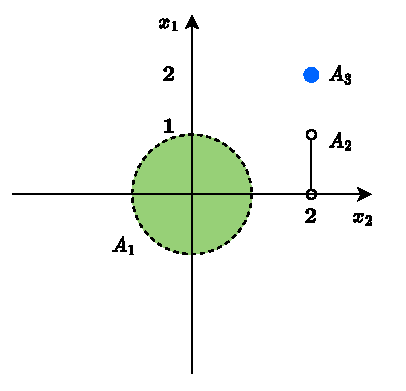
\includegraphics[width=.7\textwidth]{img/insiemi_aperti-chiusi-2.pdf}
	\end{figure}

	\begin{itemize}
		\item L'insieme dei punti interni:
		\begin{equation*}
			\mathrm{int}\left(A\right) = \mathring{A} = \left\{x \in \mathbb{R}^{2} \: : \: || x || < 1\right\} 
		\end{equation*}
		Riguardo $A_{2}$ e $A_{3}$, non hanno punti interni poiché non avendo \dquotes{area}, prendendo dei punti essi sarebbero punti di frontiera.

		\item L'insieme dei punti di frontiera:
		\begin{equation*}
			\partial A = \left\{x \in \mathbb{R}^{2} \: : \: || x || = 1\right\} \cup \left\{\left(2,t\right) \: : \: 0 \le t \le 1\right\} \cup \left\{\left(2,2\right)\right\}
		\end{equation*}
		Al contrario del precedente insieme, con i punti di frontiera si sceglie la frontiera di $A_{1}$, l'intero segmento $A_{2}$, inclusi gli estremi, e il punto $A_{3}$.

		\item La chiusura:
		\begin{equation*}
			\overline{A} = A \cup \partial A = \left\{x \in \mathbb{R}^{2} \: : \: || x || \le 1\right\} \cup \left\{\left(2,t\right) \: : \: 0 \le t \le 1\right\} \cup \left\{\left(2,2\right)\right\}
		\end{equation*}
	\end{itemize}
	L'insieme non è né aperto ($A \ne \mathring{A}$) né chiuso ($A \ne \overline{A}$).\newpage

	\begin{flushleft}
		\example{\underline{Esempio 3}}
	\end{flushleft}
	
	\noindent
	Dato l'insieme $A$:
	\begin{equation*}
		A = \left(B_{2}\left(\overrightarrow{0}\right) \setminus \left(\left[-1,1\right] \times \left\{0\right\}\right)\right) \cup \left(\left(-1,1\right) \times \left\{3\right\}\right)
	\end{equation*}
	Con la notazione $B_{2}\left(\overrightarrow{0}\right)$ si intende una palla aperta centrata in $\left(0,0\right)$ e di raggio $2$. Inoltre, è possibile riscrivere due parti dell'insieme:
	\begin{itemize}
		\item $\left(\left[-1,1\right] \times \left\{0\right\}\right)$ è una linea tratteggiata da $-1$ a $1$ (entrambi inclusi) ad altezza $0$, per cui:
		\begin{equation*}
			\left\{\left(t,0\right) \: : \: -1 \le t \le 1\right\}
		\end{equation*}

		\item $\left(\left(-1,1\right) \times \left\{3\right\}\right)$ è una linea tratteggiata da $-1$ a $1$ (entrambi esclusi) ad altezza $3$, per cui:
		\begin{equation*}
			\left\{\left(t,3\right) \: : \: -1 < t < 1\right\}
		\end{equation*}
	\end{itemize}
	La relativa rappresentazione grafica è:
	\begin{figure}[!htp]
		\centering
		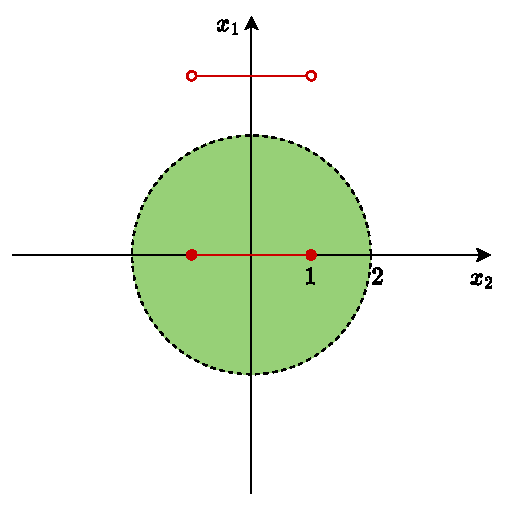
\includegraphics[width=.65\textwidth]{img/insiemi_aperti-chiusi-3.pdf}
	\end{figure}
	\begin{itemize}
		\item L'insieme dei punti interni:
		\begin{equation*}
			\mathrm{int}\left(A\right) = \mathring{A} = \left\{x \in \mathbb{R}^{2} \: : \: || x || < 2\right\} \setminus \left\{\left(t,0\right) \: : \: -1 \le t \le 1\right\}
		\end{equation*}
		Tutti quei punti interni alla palla ma escludendo la linea all'interno.

		\item L'insieme dei punti di frontiera:
		\begin{equation*}
			\partial A = \left\{x \in \mathbb{R}^{2} \: : \: || x || = 2\right\} \cup \left\{\left(t,0\right) \: : \: -1 \le t \le 1\right\} \cup \left\{\left(t,3\right) \: : \: -1 \le t \le 1\right\}
		\end{equation*}
		Tutti quei punti sulla frontiera della palla e tutte le linee fino agli estremi compresi.
		
		\item La chiusura, uguale a $A \cup \partial A$:
		\begin{equation*}
			\overline{A} = \left\{x \in \mathbb{R}^{2} \: : \: || x || \le 2\right\} \cup \left\{\left(t,0\right) \: : \: -1 \le t \le 1\right\} \cup \left\{\left(t,3\right) \: : \: -1 \le t \le 1\right\}
		\end{equation*}
		L'insieme non è aperto né aperto ($A \ne \mathring{A}$), né chiuso ($A \ne \overline{A}$).
	\end{itemize}\newpage

	\begin{flushleft}
		\example{\underline{Esempio 4}}
	\end{flushleft}

	\noindent
	Dato l'insieme $A$:
	\begin{equation*}
		A = \left\{\left(x,y\right) \in \mathbb{R}^{2} \: : \: \max\left\{|x|, |y|\right\} \ge 3, \: x^{2}+y^{2} \le 16\right\}
	\end{equation*}
	In questo caso è possibile osservare delle cose interessanti. La funzione $\max$ sceglie il valore massimo tra i due proposti e tale valore deve essere maggiore o uguale a $3$. Questo significa che è necessario disegnare un quadrato dato che potenzialmente il valore potrebbe andare all'infinito (vedi la figura a pagina \pageref{fig: alcune rappresentazioni di norme in due dimensioni} in cui si mostrano alcune norme a due dimensioni).

	Negli esempi precedenti, è sempre stato chiesto di rappresentare delle norme ben definite. In questo caso, viene fornita un'equazione di una circonferenza (le formule si trovano nel paragrafo \ref{subsubsection: circonferenza}), che rappresenta una palla chiusa ($\le$) di raggio $r = 4$ $\left(\sqrt{16}\right)$ e centro $\left(0,0\right)$ (mancano gli altri valori rispetto l'equazione canonica).\newline

	\noindent
	Quindi, la sua rappresentazione grafica:
	\begin{figure}[!htp]
		\centering
		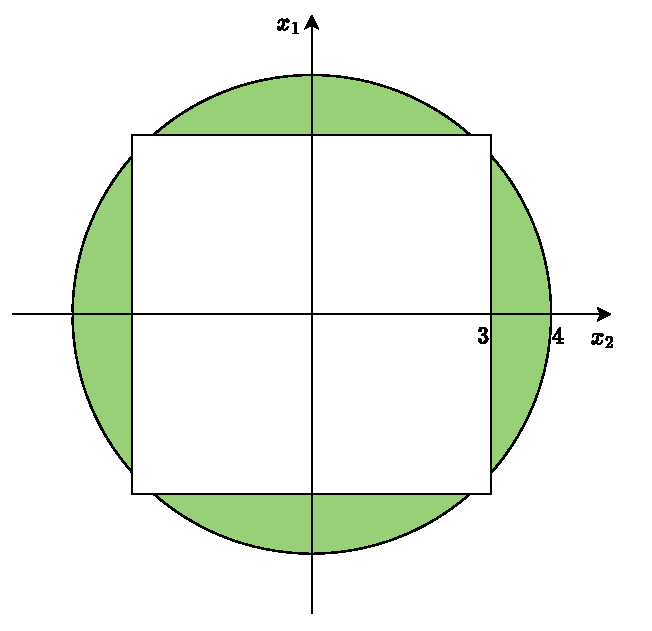
\includegraphics[width=.7\textwidth]{img/insiemi_aperti-chiusi-4.pdf}
	\end{figure}
	\begin{itemize}
		\item L'insieme dei punti interni:
		\begin{equation*}
			\mathrm{int}\left(A\right) = \mathring{A} =\left\{\left(x,y\right) \in \mathbb{R}^{2} \: : \: \max\left\{|x|, |y|\right\} > 3, \: x^{2}+y^{2} < 16\right\}
		\end{equation*}
		
		\item L'insieme dei punti di frontiera:
		\begin{equation*}
			\partial A = \left\{\left(x,y\right) \in \mathbb{R}^{2} \: : \: \max\left\{|x|, |y|\right\} = 3, \: x^{2}+y^{2} = 16\right\}
		\end{equation*}

		\item La chiusura, uguale a $A \cup \partial A$, è identica ad $A$ poiché è già presente l'uguale nelle condizioni.
	\end{itemize}
	L'insieme non è aperto perché $A \ne \mathring{A}$, ma è chiuso poiché $A = \overline{A}$.

	\subsection{Funzioni da \texorpdfstring{$\mathbb{R}^{n}$}{Rn} in \texorpdfstring{$\mathbb{R}$}{R} (funzioni scalari)}\label{subsection: funzioni da R^n in R (funzioni scalari)}

	Le funzioni da $\mathbb{R}^{n}$ in $\mathbb{R}$, vengono chiamate \definition{funzioni scalari}. Associando ad ogni $n$-upla di numeri reali in un insieme $D$ un unico numero reale in base a una specifica regola, si definisce una funzione da $D$ a $\mathbb{R}$:
	\begin{equation}
		\begin{array}{rcl}
			f \: : \: D \subseteq \mathbb{R}^{n} &\rightarrow& \mathbb{R} \\
			x &\mapsto& f\left(x\right)
		\end{array}
	\end{equation}
	In particolare, con $n = 2$, si può ridurre alla seguente forma:
	\begin{equation}
		\begin{array}{rcl}
			f \: : \: D \subseteq \mathbb{R}^{2} &\rightarrow& \mathbb{R} \\
			\left(x,y\right) &\mapsto& z = f\left(x,y\right)
		\end{array}
	\end{equation}
	In cui le variabili $x$ e $y$ sono indipendenti, mentre la variabile $z$ è dipendente.

	\longline

	\subsubsection{Rappresentazione grafica del dominio di funzioni (\texorpdfstring{$n = 2$}{n = 2})}\label{subsubsection: rappresentazione grafica del dominio di funzioni (n = 2)}

	Determinare e rappresentare il dominio delle seguenti funzioni:
	\begin{enumerate}
		\item $f\left(x,y\right) = x\ln\left(x-y\right)$
		\item $f\left(x,y\right) = \sqrt{x-3} + \sqrt{y+1} - \sqrt{x^{2} + y^{2}}$
		\item $f\left(x,y\right) = \sqrt{4x^{2} + y^{2} - 4}$
		\item $f\left(x,y\right) = \sqrt{x+y+1} - \ln\left(x^{2} - y\right)$
		\item $f\left(x,y\right) = \arccos\left(xy\right)$
		\item $f\left(x,y\right) = \dfrac{\ln\left(1-x^{2}-y^{2}\right)}{\sqrt{x}}$ 
		\item $f\left(x,y,z\right) = \dfrac{1}{y^{2} + z^{2} - 4}$
	\end{enumerate}\newpage

	\begin{flushleft}
		\example{\underline{Esempio 1}}
	\end{flushleft}

	\noindent
	Data la funzione:
	\begin{equation*}
		f\left(x,y\right) = x\ln\left(x-y\right)
	\end{equation*}
	L'unica condizione d'esistenza è data dal logaritmo, il quale deve avere l'argomento maggiore di zero. Per cui, il dominio della funzione è:
	\begin{equation*}
		D = \left\{\left(x,y\right) \in \mathbb{R}^{2} \: : \: x-y > 0\right\}
	\end{equation*}
	Per rappresentarlo, si può manipolare velocemente la disuguaglianza:
	\begin{equation*}
		x-y>0 \rightarrow x > y
	\end{equation*}
	Nel caso in cui fosse $x = y$, il grafico sarebbe una retta, ma in questo caso c'è il maggiore. Di conseguenza, la retta deve essere tratteggiata e il dominio di interesse è quello sotto la retta:
	\begin{figure}[!htp]
		\centering
		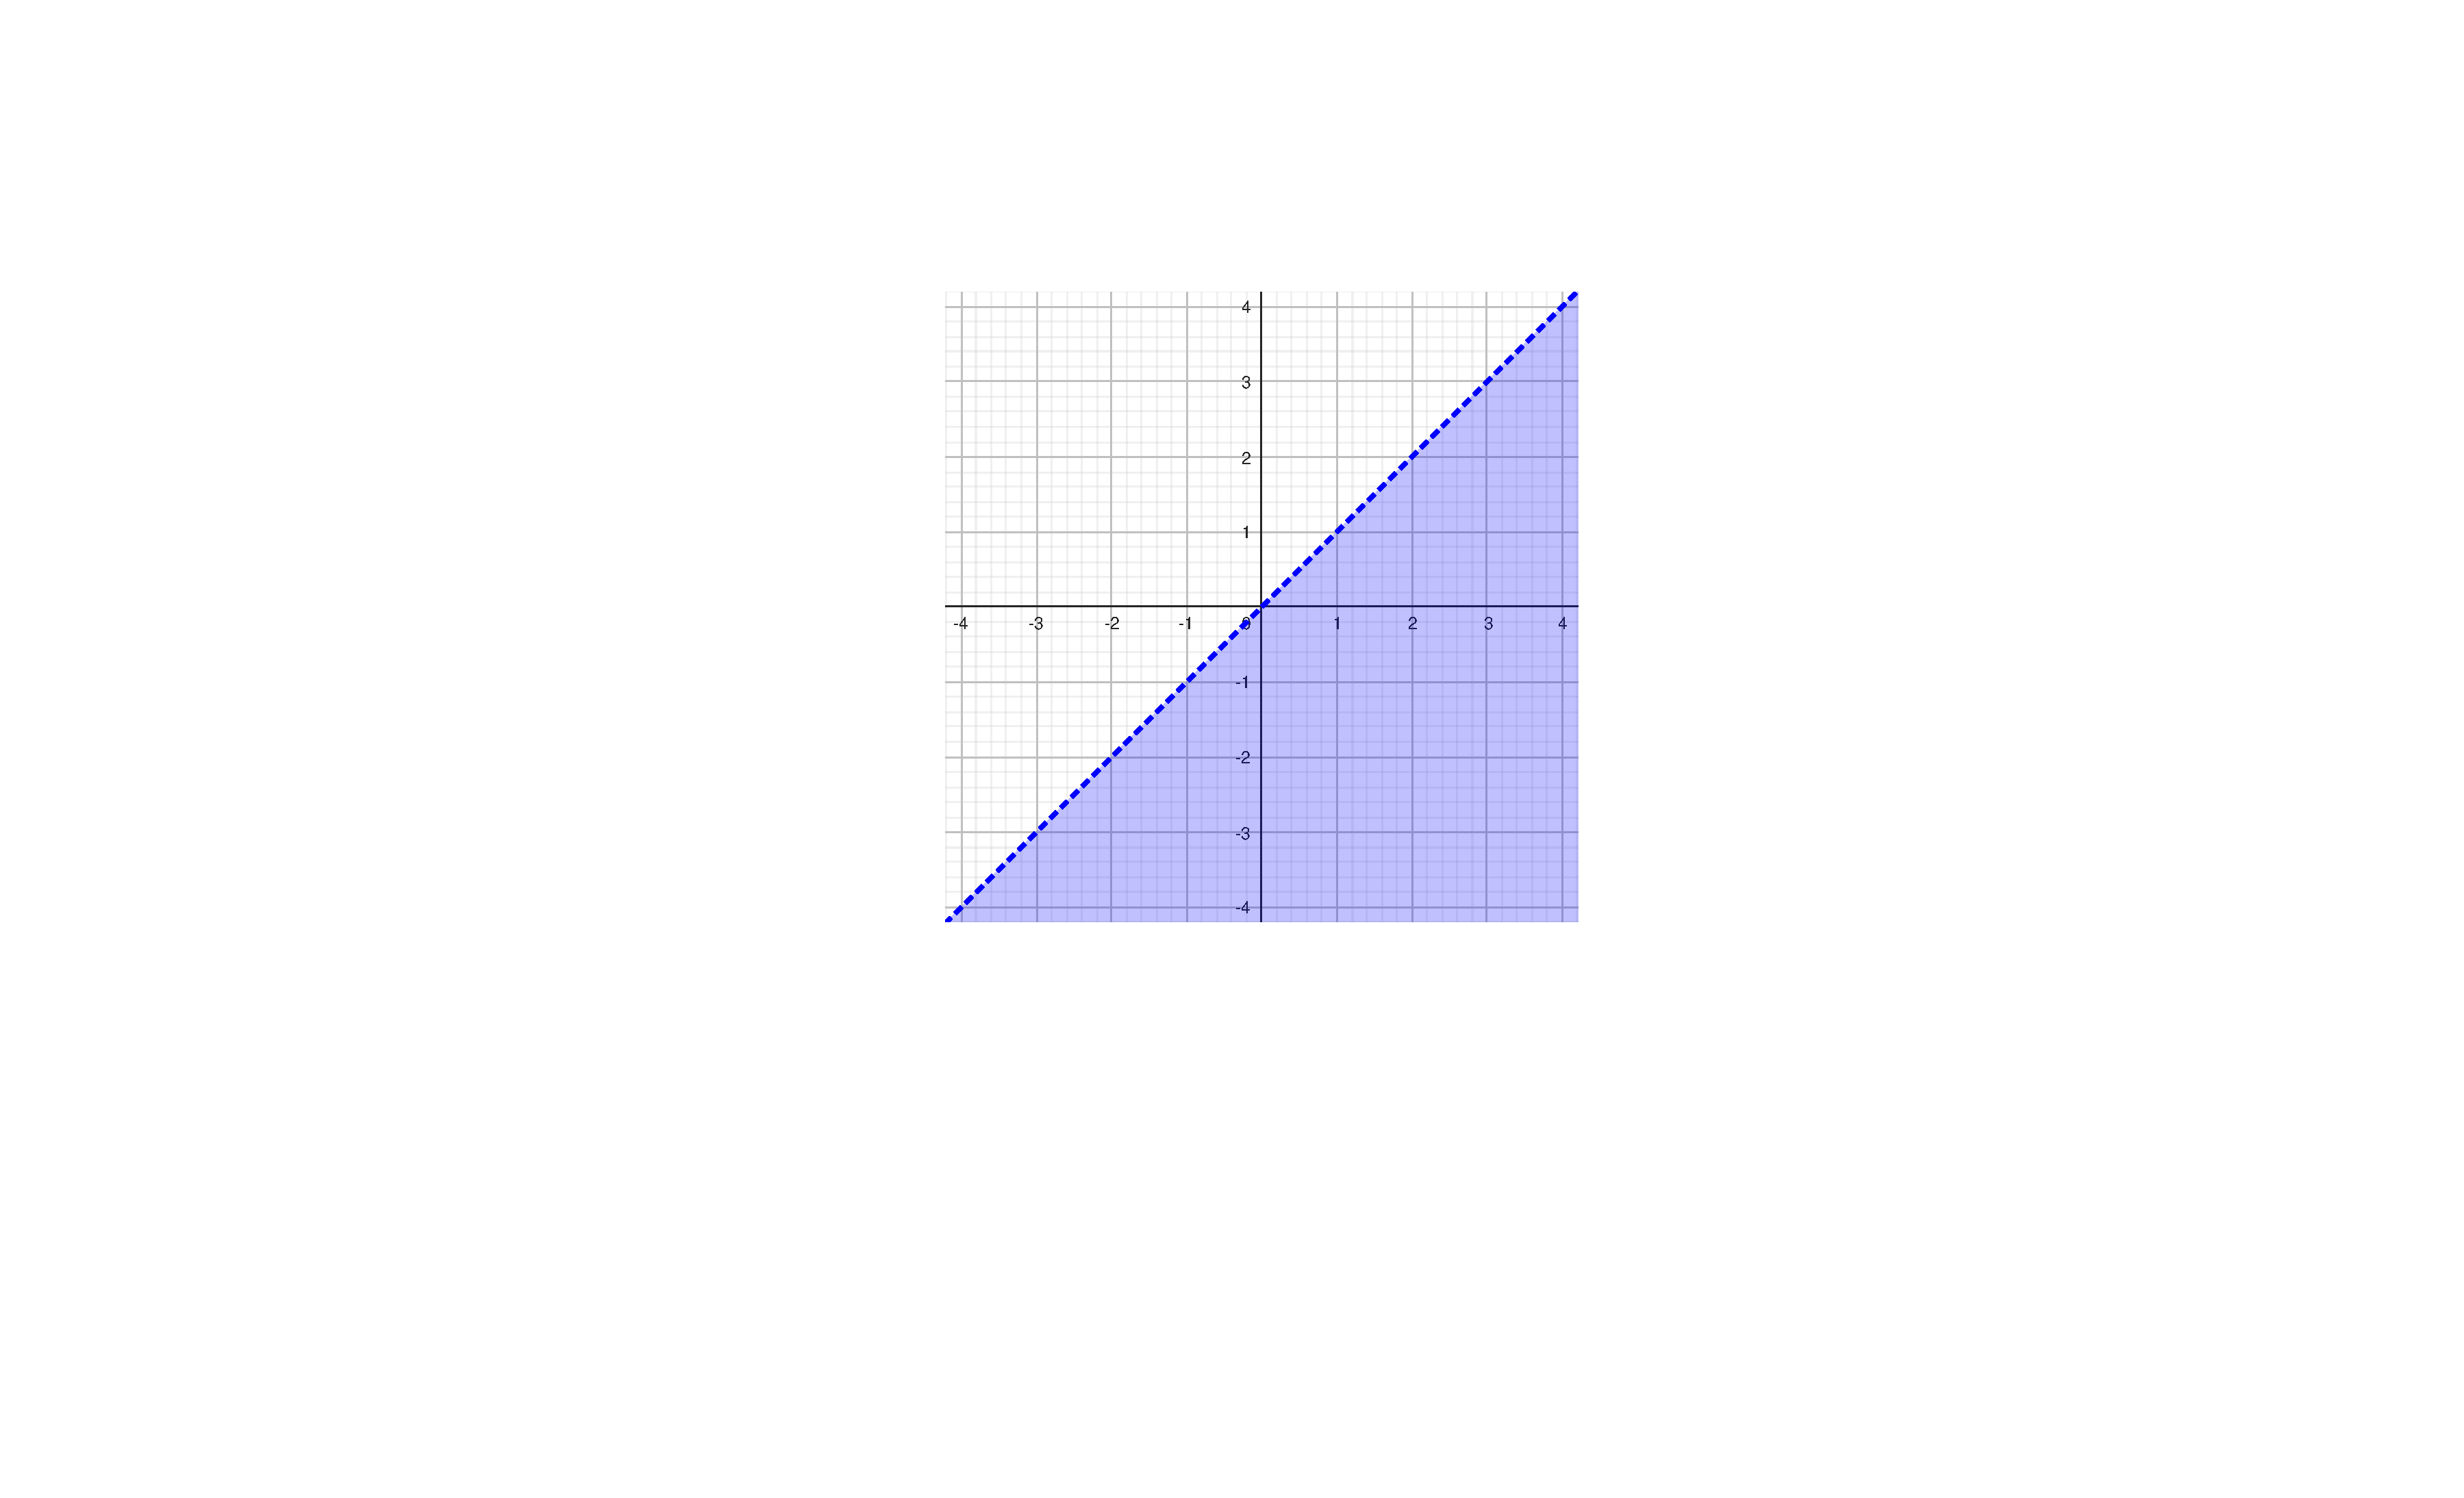
\includegraphics[width=.7\textwidth]{img/dominio_di_funzioni-1.pdf}
	\end{figure}
	\begin{itemize}
		\item L'insieme dei punti interni:
		\begin{equation*}
			\mathrm{int}\left(D\right) = \mathring{D} = \left\{\left(x,y\right) \in \mathbb{R}^{2} \: : \: x-y > 0\right\}
		\end{equation*}

		\item L'insieme dei punti di frontiera:
		\begin{equation*}
			\partial D = \left\{\left(x,y\right) \in \mathbb{R}^{2} \: : \: x - y = 0\right\}
		\end{equation*}

		\item La chiusura:
		\begin{equation*}
			\overline{D} = D \cup \partial D = \left\{\left(x,y\right) \in \mathbb{R}^{2} \: : \: x - y \ge 0\right\}
		\end{equation*}
	\end{itemize}
	L'insieme $D$ è aperto poiché $D = \mathring{D}$ e non è chiuso poiché $D \ne \overline{D}$.\newpage

	\begin{flushleft}
		\example{\underline{Esempio 2}}
	\end{flushleft}

	\noindent
	Data la funzione:
	\begin{equation*}
		f\left(x,y\right) = \sqrt{x-3} + \sqrt{y+1} - \sqrt{x^{2} + y^{2}}
	\end{equation*}
	Le condizioni d'esistenza sono i valori sotto le radici, i quali devono essere maggiori uguali a zero per evitare di entrare nell'insieme dei numeri immaginari. Per cui, il dominio della funzione è:
	\begin{equation*}
		D = \left\{\left(x,y\right) \in \mathbb{R}^{2} \: : \: x-3 \ge 0 \: \land \: y+1 \ge 0 \: \land \: x^{2}+y^{2} \ge 0\right\}
	\end{equation*}
	Per rappresentarlo, si possono manipolare velocemente la disuguaglianze:
	\begin{itemize}
		\item $x-3 \ge 0 \rightarrow x \ge 3$

		\item $y+1 \ge 0 \rightarrow y \ge -1$
	\end{itemize}
	La rappresentazione delle due rette è immediato. Si prende in considerazione il piano da $x$ maggiore/uguale di $3$ in poi e da $y$ maggiore uguale di $-1$ in poi. Per quanto riguarda $x^{2} + y^{2}$, non si prende in considerazione poiché la disuguaglianza è sempre verificata dato che un numero reale elevato al quadrato non potrà mai essere negativo (figuriamoci una somma tra due numeri reali al quadrato).
	\begin{figure}[!htp]
		\centering
		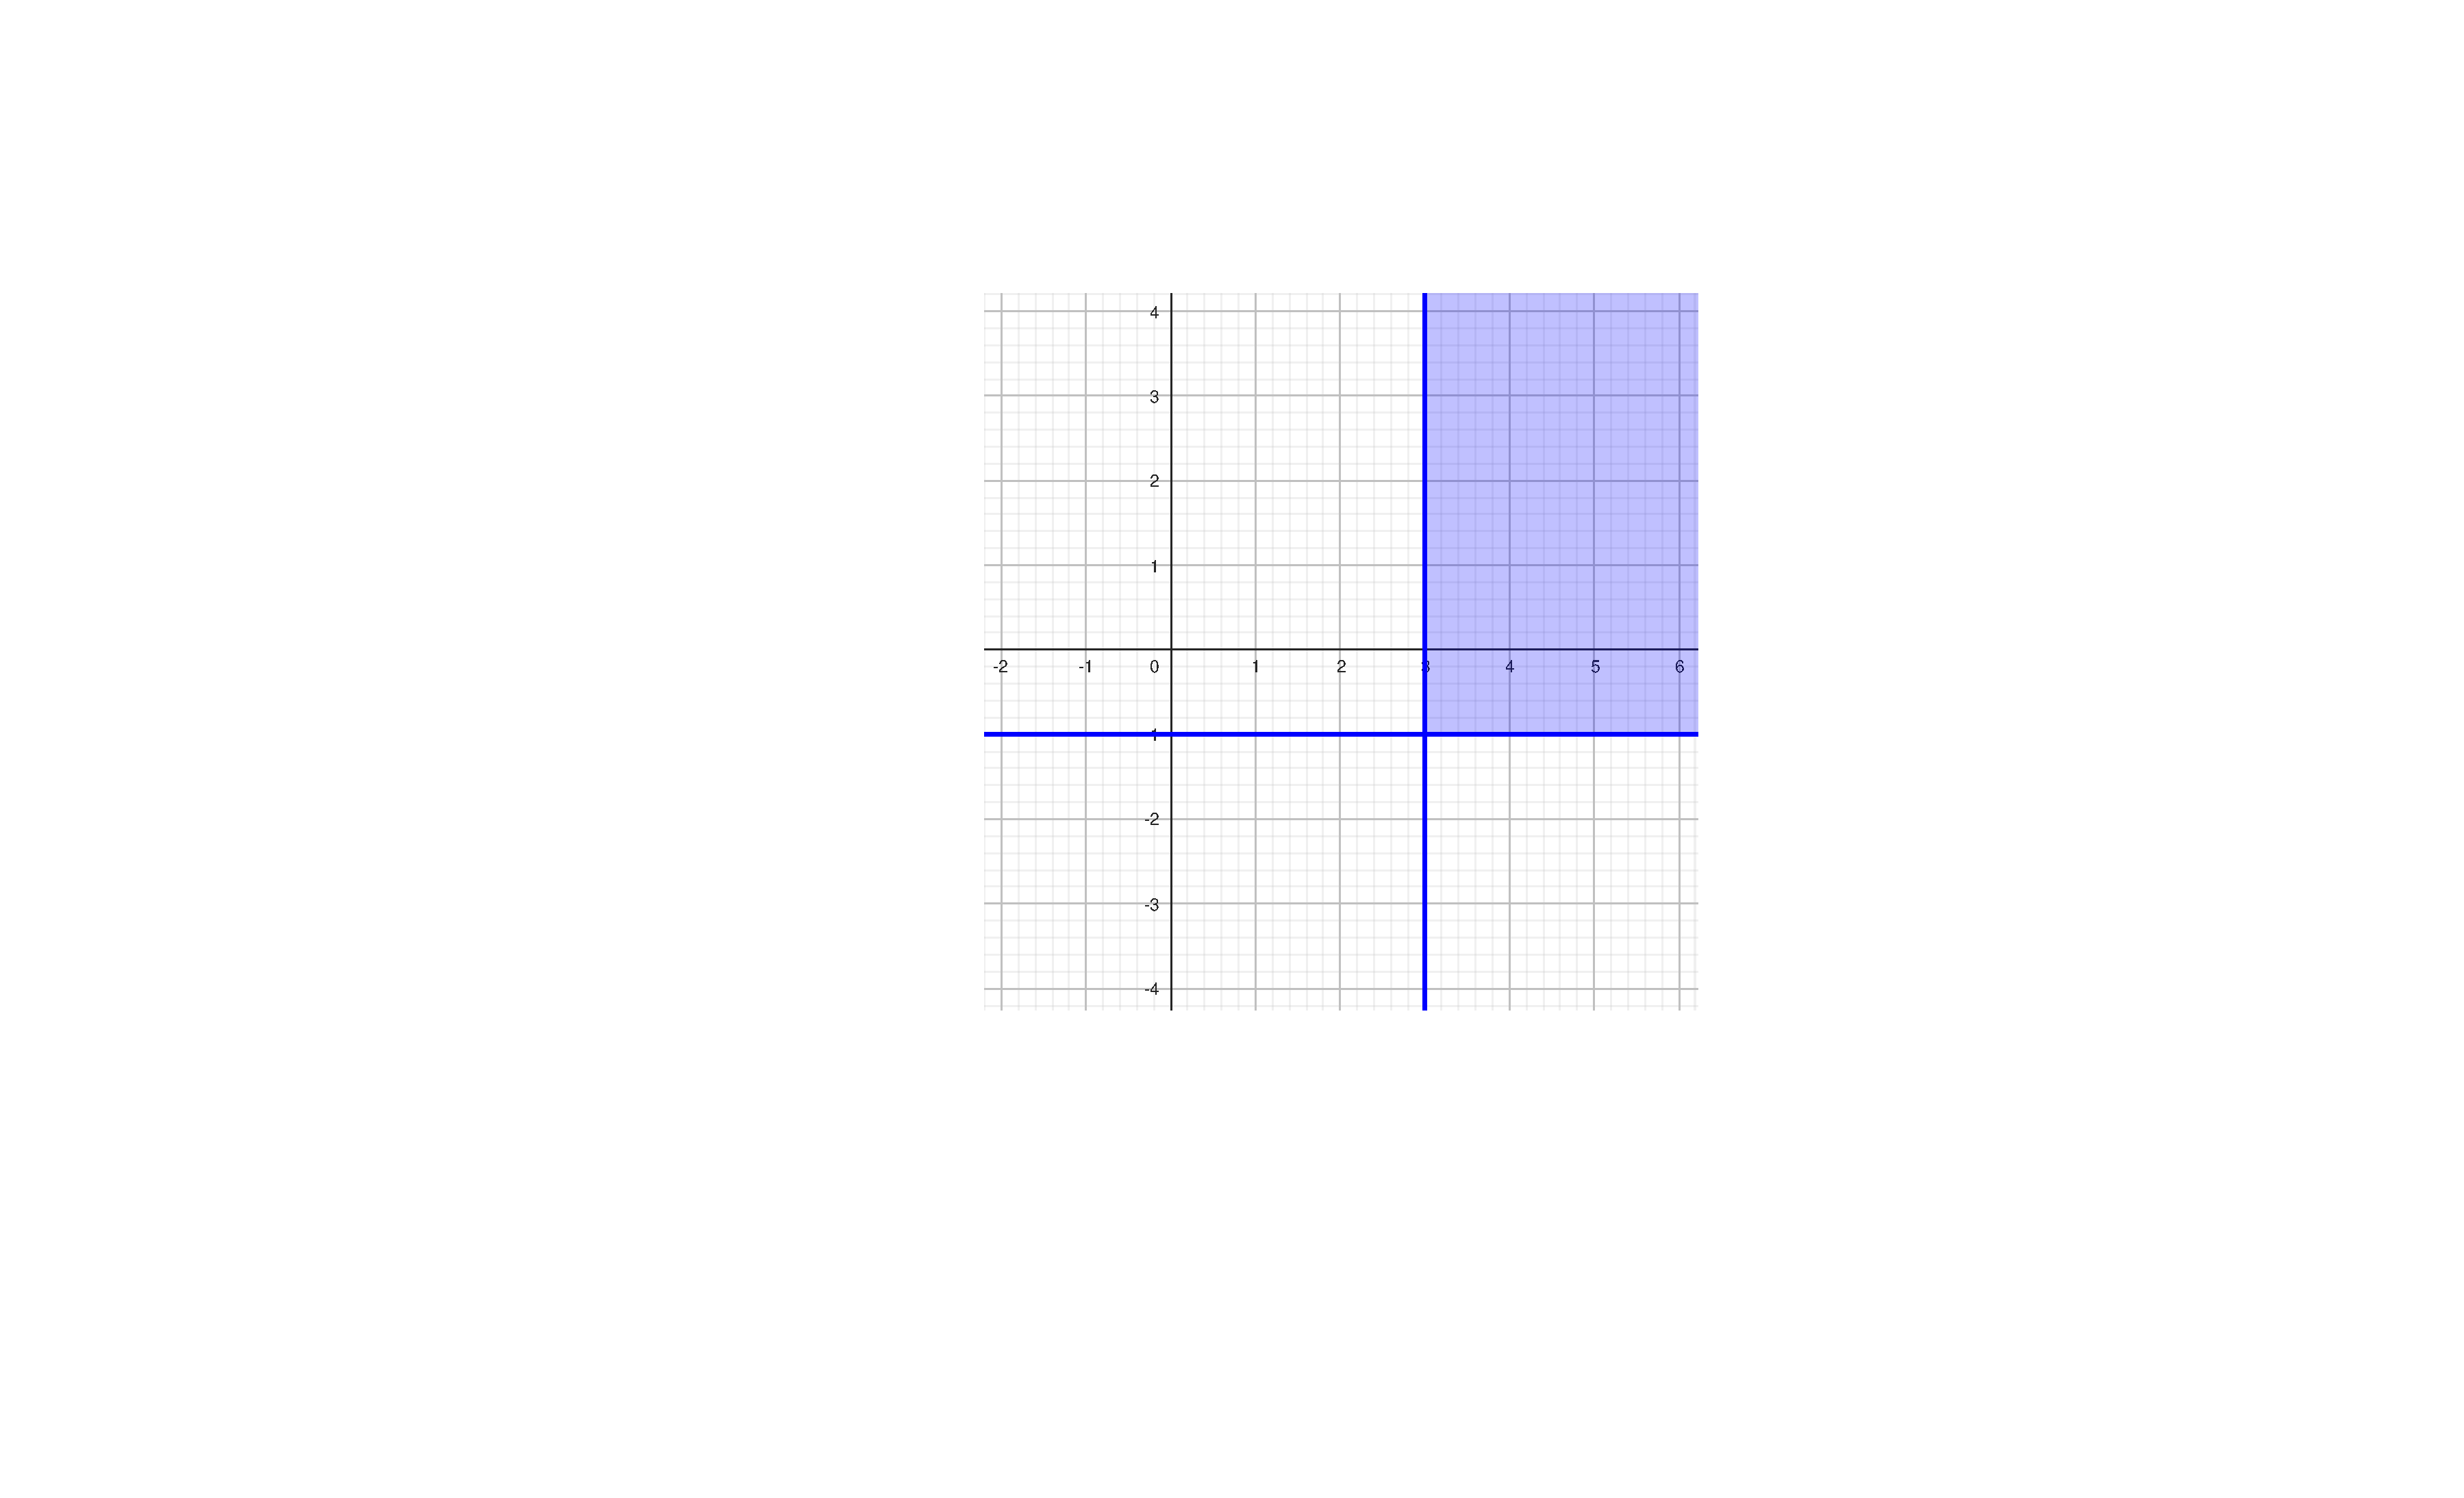
\includegraphics[width=.6\textwidth]{img/dominio_di_funzioni-2.pdf}
	\end{figure}
	\begin{itemize}
		\item L'insieme dei punti interni:
		\begin{equation*}
			\mathrm{int}\left(D\right) = \mathring{D} = \left\{\left(x,y\right) \in \mathbb{R}^{2} \: : \: x > 3 \: \land \: y > 1\right\}
		\end{equation*}

		\item L'insieme dei punti di frontiera:
		\begin{equation*}
			\partial D = \left\{\left(x,y\right) \in \mathbb{R}^{2} \: : \: x = 3 \: \land \: y = -1\right\}
		\end{equation*}

		\item La chiusura:
		\begin{equation*}
			\overline{D} = D \cup \partial D = \left\{\left(x,y\right) \in \mathbb{R}^{2} \: : \: x \ge 3 \: \land \: y \ge -1\right\}
		\end{equation*}
	\end{itemize}
	L'insieme $D$ non è aperto poiché $D \ne \mathring{D}$ ma è chiuso poiché $D = \overline{D}$.\newpage

	\begin{flushleft}
		\example{\underline{Esempio 3}}
	\end{flushleft}

	\noindent
	Data la funzione:
	\begin{equation*}
		f\left(x,y\right) = \sqrt{4x^{2} + y^{2} - 4}
	\end{equation*}
	La condizione d'esistenza è il valore sotto radice, quindi il dominio è:
	\begin{equation*}
		D = \left\{\left(x,y\right) \in \mathbb{R}^{2} \: : \: 4x^{2} + y^{2} - 4 \ge 0\right\}
	\end{equation*}
	In questo caso, dato che la disuguaglianza non è sempre vera come nell'esempio precedente, è necessario rappresentare l'ellisse (paragrafo \ref{subsubsection: ellisse}) utilizzando l'equazione canonica che si ricava:
	\begin{equation*}
		4x^{2} + y^{2} - 4 \ge 0 \rightarrow 4x^{2} + y^{2} \ge 4 \rightarrow \dfrac{x^{2}}{1} + \dfrac{y^{2}}{4} = 1
	\end{equation*}
	La rappresentazione dell'ellisse non è complessa. Sapendo che è centrata nell'origine, i vertici vengono calcolati nel seguente modo. Riguardo l'asse $x$, l'ellisse intersecherà su $\pm 1$, mentre sull'asse delle $y$ intersecherà su $\pm 2$ ($\sqrt{4}$, si ricorda che i valori al denominatore vengono considerati al quadrato secondo la forma canonica). Infine, dopo aver disegnato l'ellisse, si considera l'esterno e il bordo poiché la condizione è maggiore o uguale.
	\begin{figure}[!htp]
		\centering
		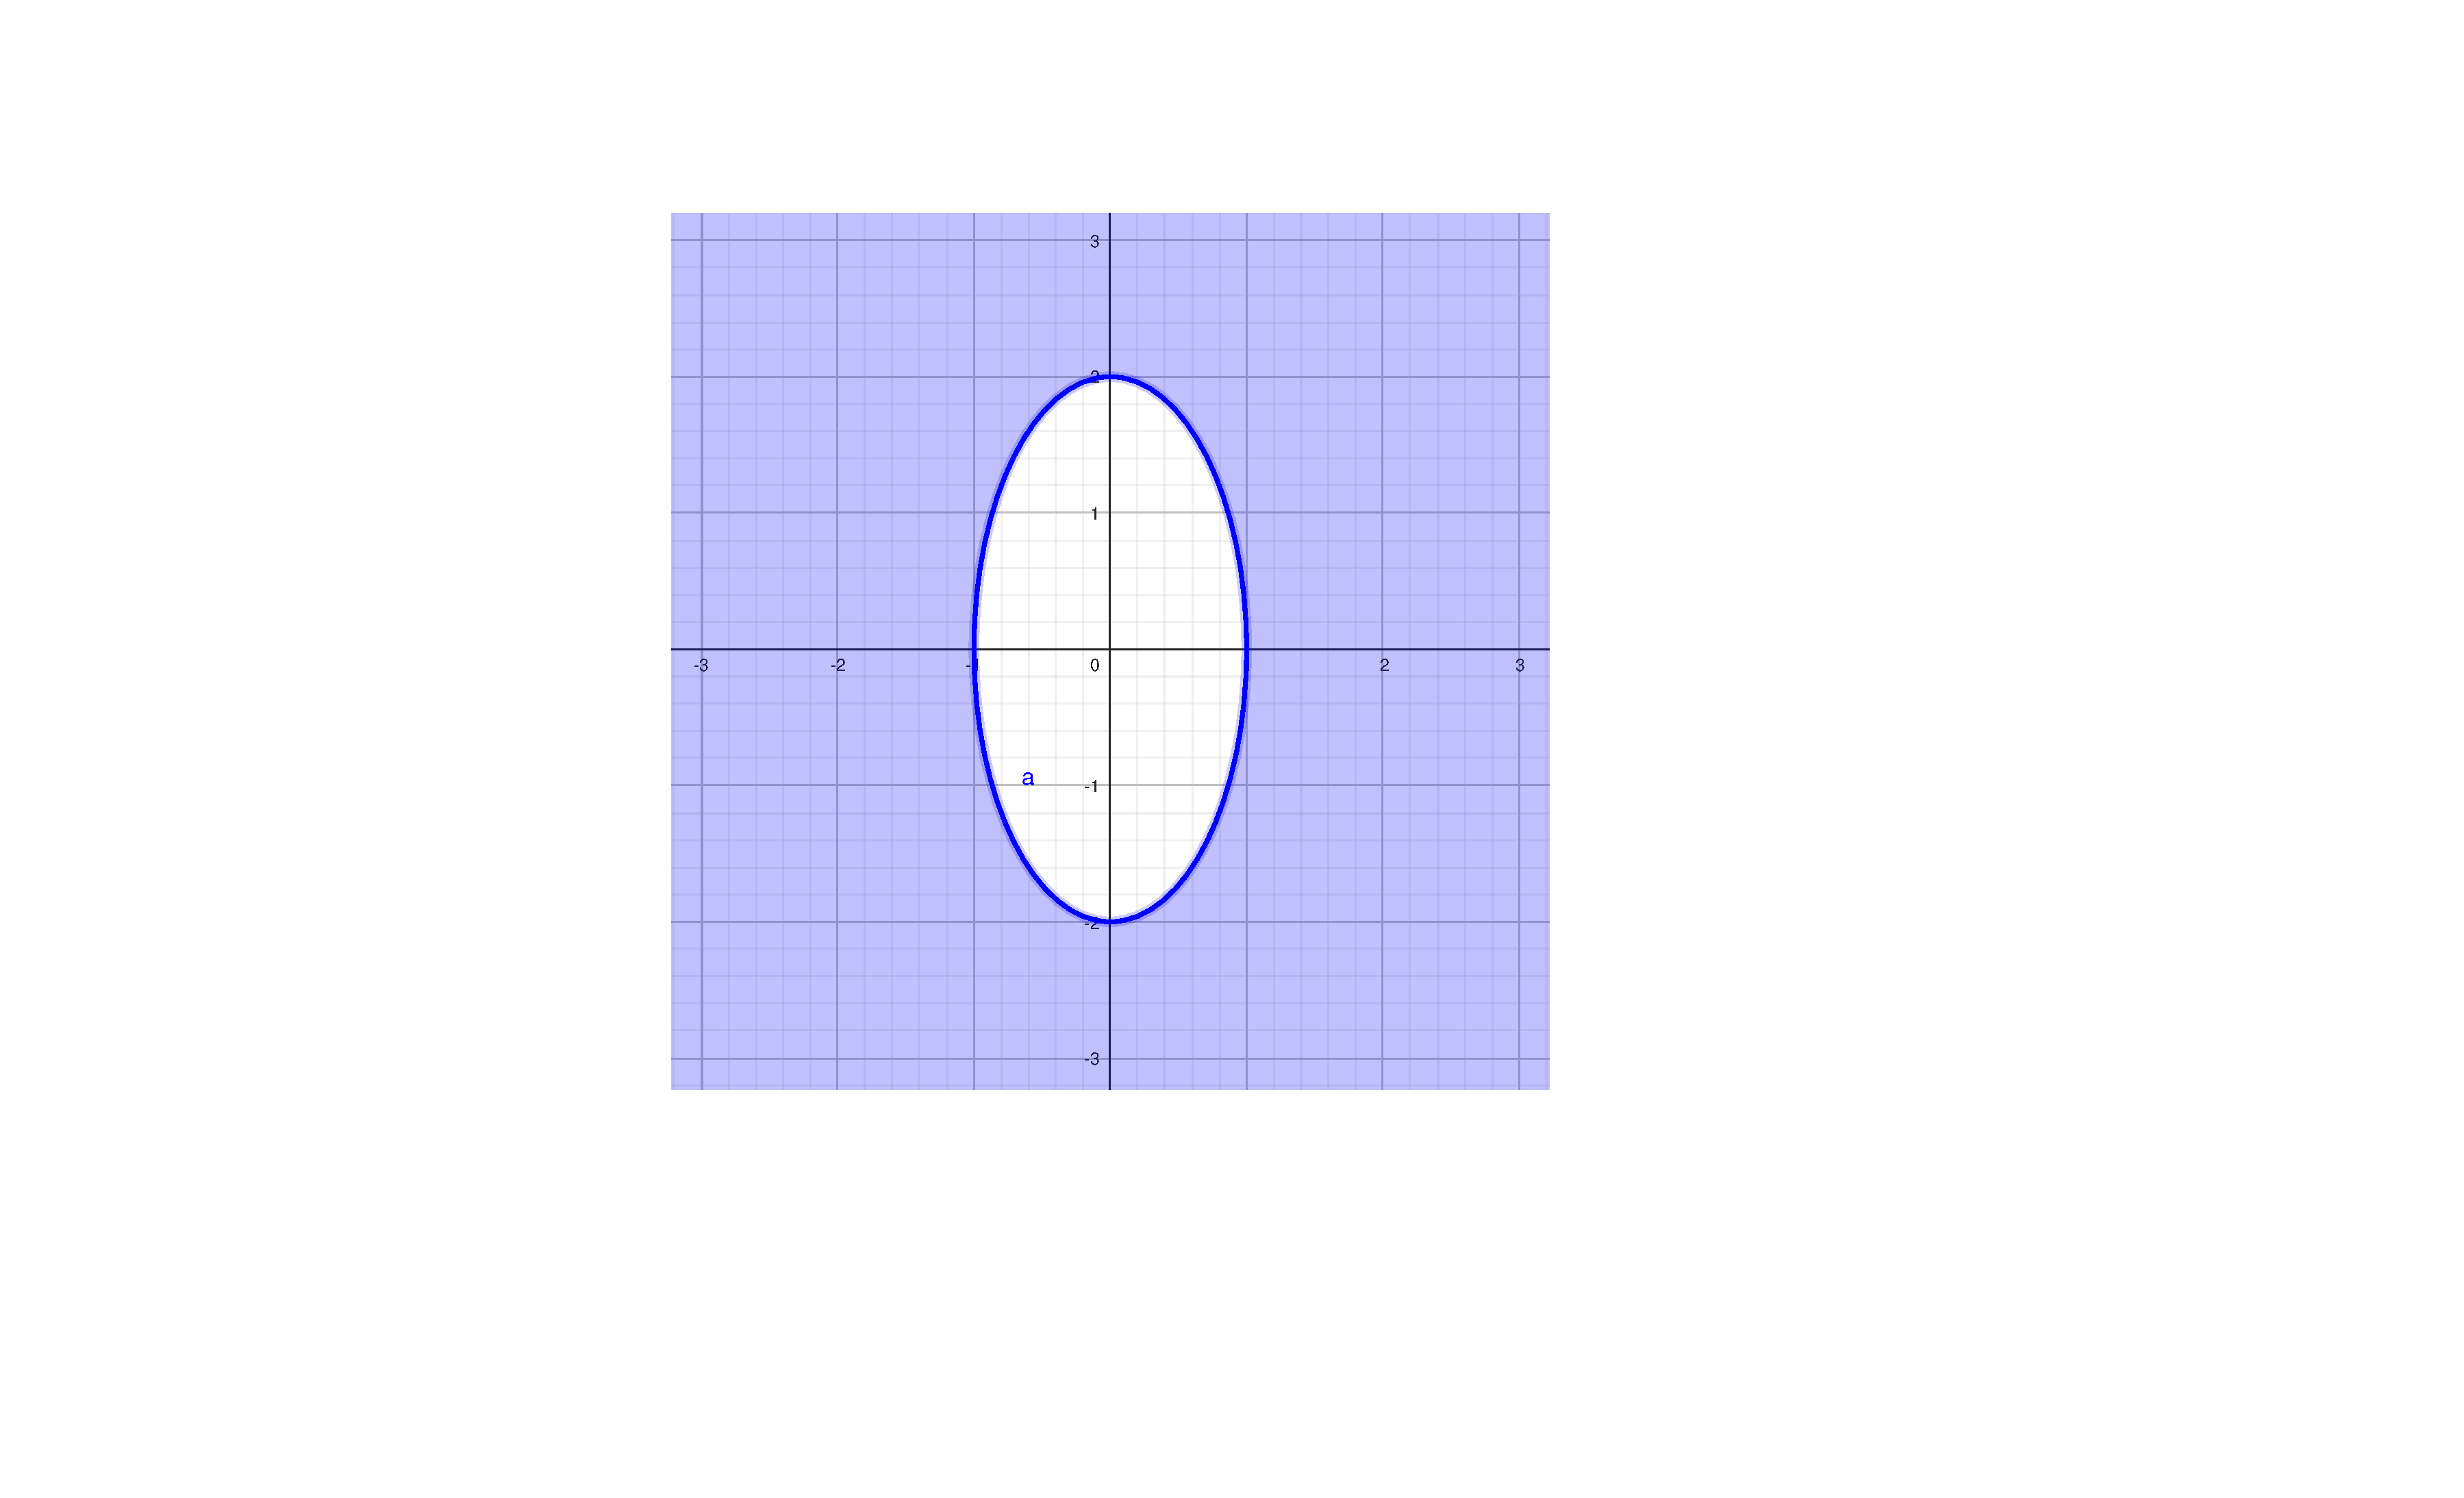
\includegraphics[width=.63\textwidth]{img/dominio_di_funzioni-3.pdf}
	\end{figure}
	\begin{itemize}
		\item L'insieme dei punti interni:
		\begin{equation*}
			\mathrm{int}\left(D\right) = \mathring{D} = \left\{\left(x,y\right) \in \mathbb{R}^{2} \: : \: 4x^{2} + y^{2} - 4 > 0\right\}
		\end{equation*}

		\item L'insieme dei punti di frontiera:
		\begin{equation*}
			\partial D = \left\{\left(x,y\right) \in \mathbb{R}^{2} \: : \: 4x^{2} + y^{2} - 4 = 0\right\}
		\end{equation*}

		\item La chiusura:
		\begin{equation*}
			\overline{D} = D \cup \partial D = \left\{\left(x,y\right) \in \mathbb{R}^{2} \: : \: 4x^{2} + y^{2} - 4 \ge 0\right\}
		\end{equation*}
	\end{itemize}
	L'insieme $D$ non è aperto poiché $D \ne \mathring{D}$ ma è chiuso poiché $D = \overline{D}$.\newpage

	\begin{flushleft}
		\example{\underline{Esempio 4}}
	\end{flushleft}

	\noindent
	Data la funzione:
	\begin{equation*}
		f\left(x,y\right) = \sqrt{x+y+1} - \ln\left(x^{2} - y\right)
	\end{equation*}
	La condizione d'esistenza è il valore sotto radice e il logaritmo:
	\begin{equation*}
		D = \left\{\left(x,y\right) \in \mathbb{R}^{2} \: : \: x+y+1 \ge 0 \: \land \: x^{2}-y > 0\right\}
	\end{equation*}
	In questo caso, la prima disuguaglianza è semplice. Sarebbe come dire $x$ deve essere l'opposto di $y$ ($x = -y$), ma con $y$ che poi viene incrementata di $1$. Per cui, se $x = 1$, la $y = -1 + 1$, cioè $0$. Invece, per la seconda dovrebbe essere immediato il fatto che sia un'iperbole. Difatti, se $x=\pm1^{2}$, allora $y = 1$, se $x=\pm2^{2}=4$ allora $y=4$ e così via.
	\begin{figure}[!htp]
		\centering
		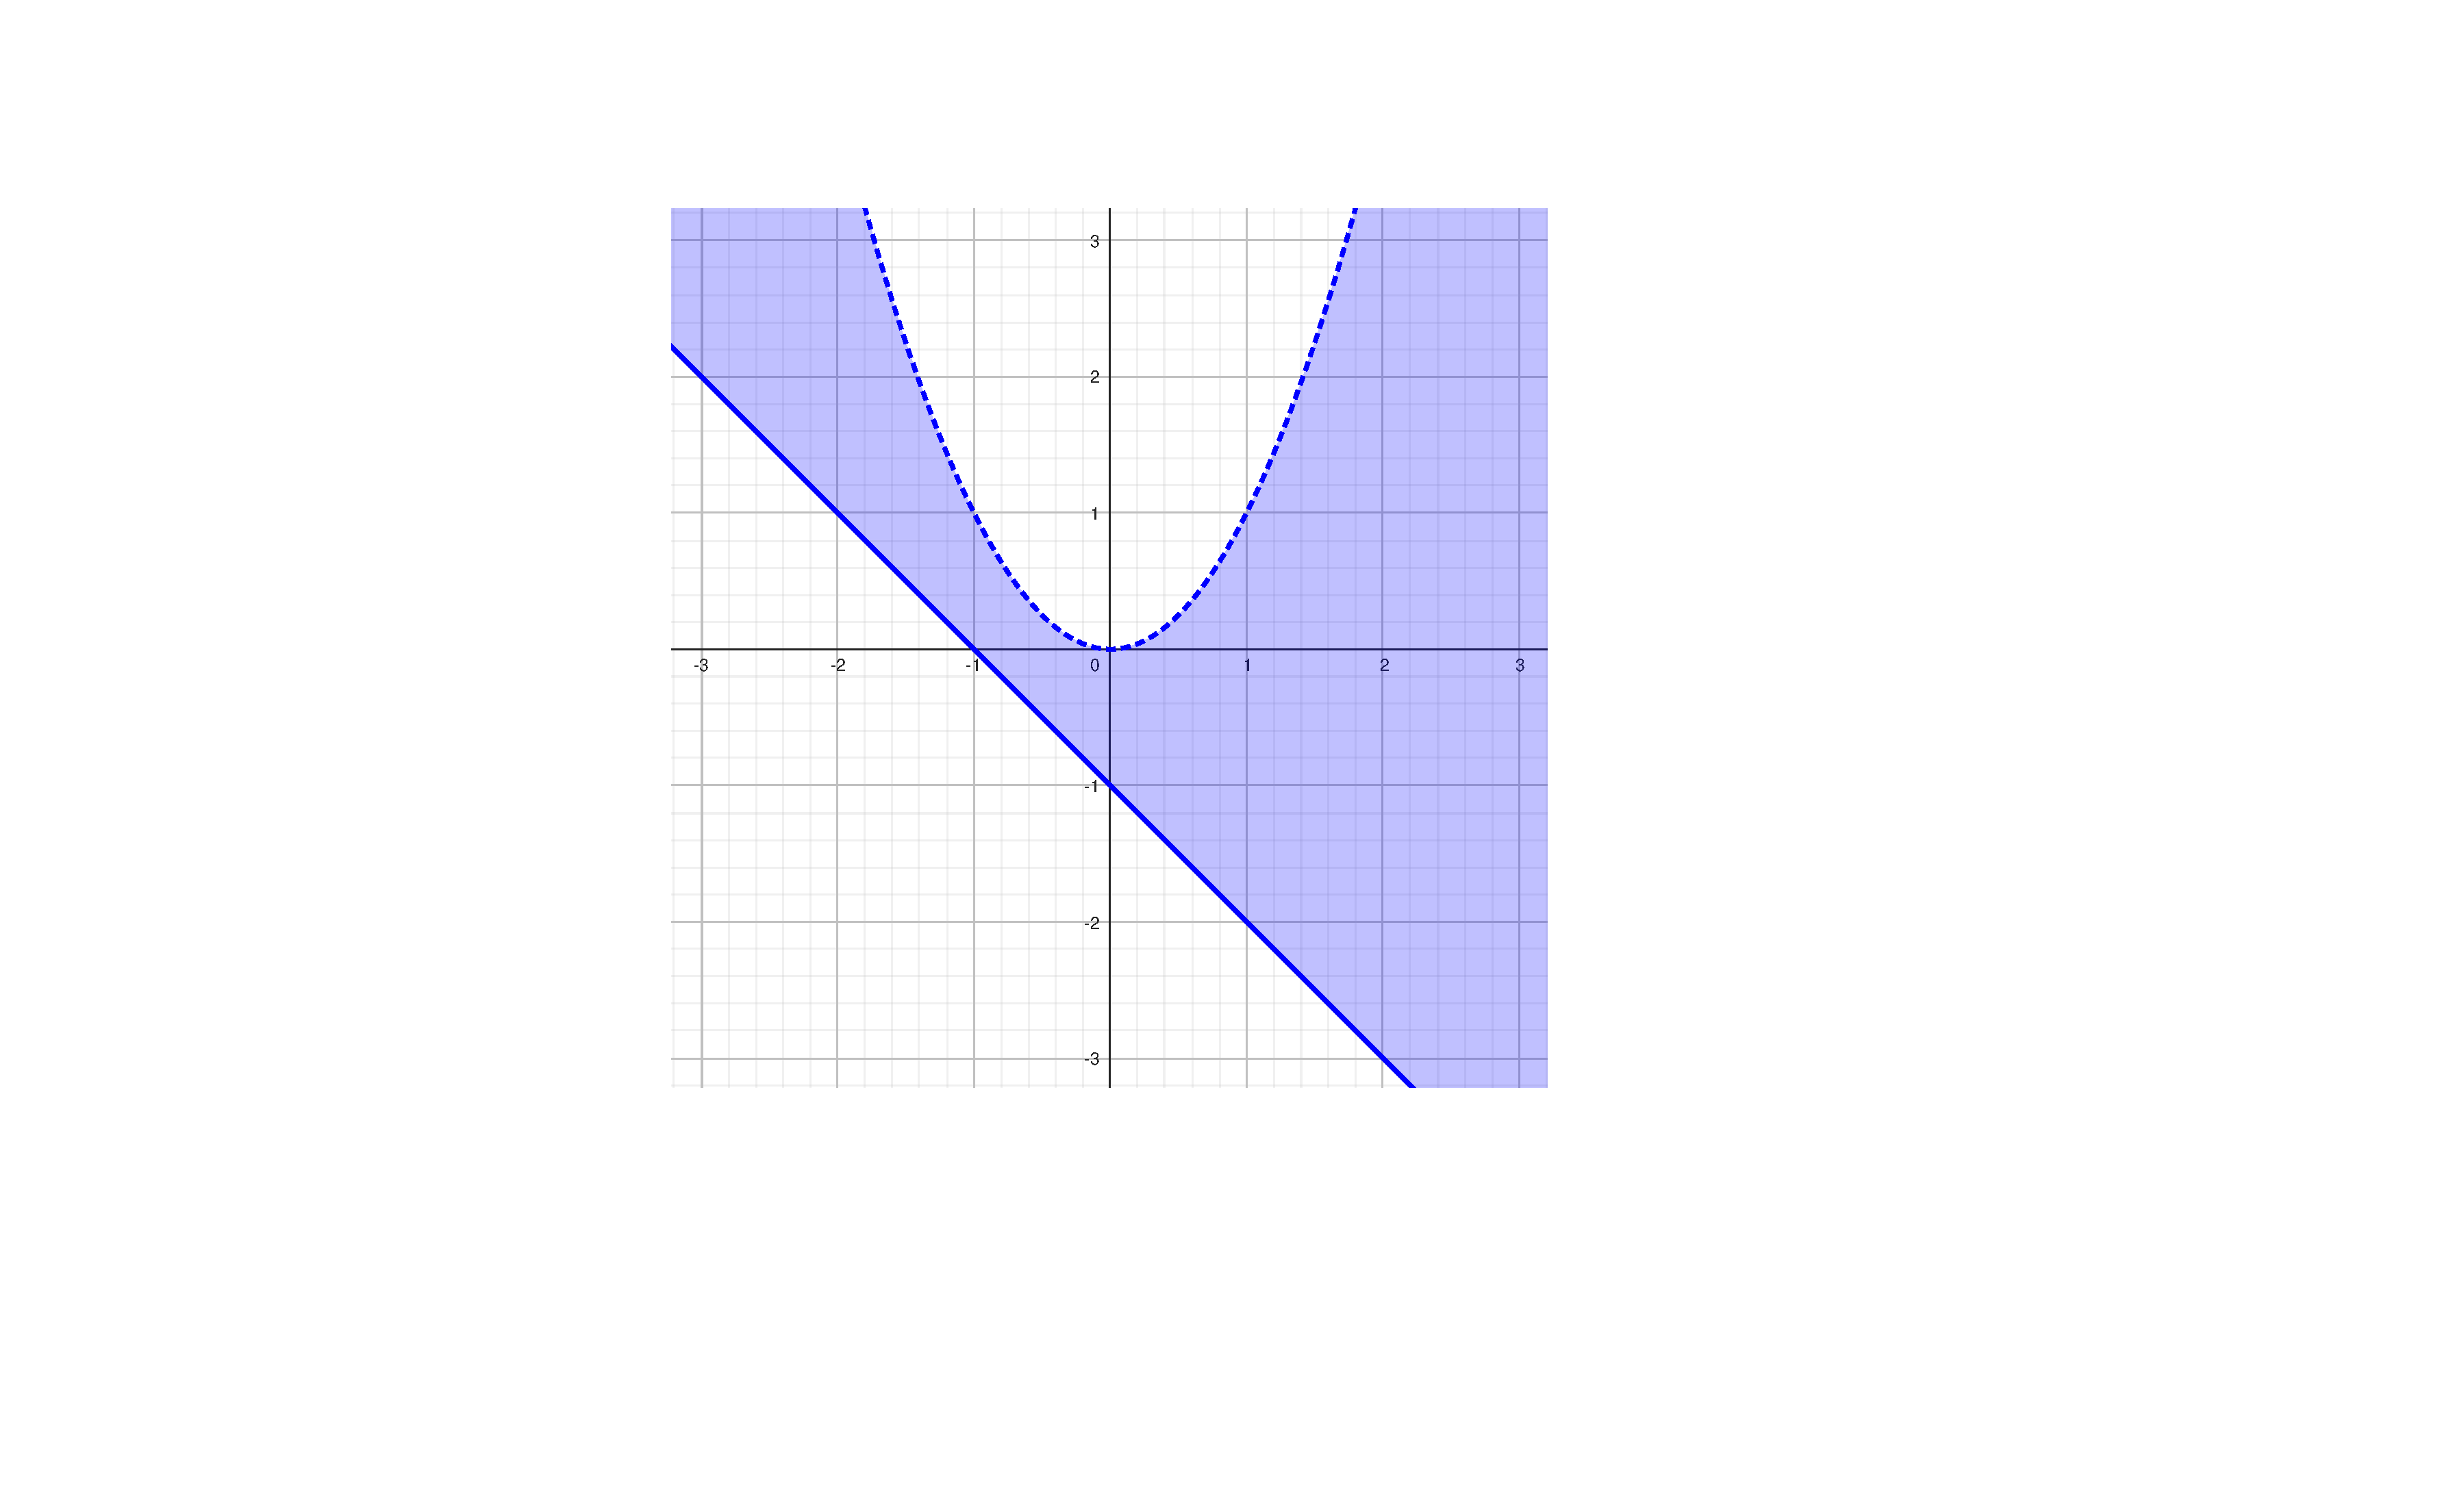
\includegraphics[width=.7\textwidth]{img/dominio_di_funzioni-4.pdf}
	\end{figure}
	\begin{itemize}
		\item L'insieme dei punti interni:
		\begin{equation*}
			\mathrm{int}\left(D\right) = \mathring{D} = \left\{\left(x,y\right) \in \mathbb{R}^{2} \: : \: x+y+1 > 0 \: \land \: x^{2}-y > 0\right\}
		\end{equation*}

		\item L'insieme dei punti di frontiera:
		\begin{equation*}
			\partial D = \left\{\left(x,y\right) \in \mathbb{R}^{2} \: : \: x+y+1 = 0 \: \land \: x^{2}-y = 0\right\}
		\end{equation*}

		\item La chiusura:
		\begin{equation*}
			\overline{D} = D \cup \partial D = \left\{\left(x,y\right) \in \mathbb{R}^{2} \: : \: x+y+1 \ge 0 \: \land \: x^{2}-y \ge 0\right\}
		\end{equation*}
	\end{itemize}
	L'insieme $D$ non è aperto poiché $D \ne \mathring{D}$ ma neanche chiuso poiché $D \ne \overline{D}$.\newpage

	\begin{flushleft}
		\example{\underline{Esempio 5}}
	\end{flushleft}

	\noindent
	Data la funzione:
	\begin{equation*}
		f\left(x,y\right) = \arccos\left(xy\right)
	\end{equation*}
	La funzione $\arccos$ corrisponde a $\alpha = \arccos\left(xy\right)$ ovvero $\cos\left(\alpha\right) = xy$. Ricordando (\href{https://www.youmath.it/lezioni/analisi-matematica/le-funzioni-elementari-e-le-loro-proprieta/376-arcocoseno.html}{approfondimento}) che la funzione $\arccos$ ha il suo argomento, in questo caso $xy$, definito nell'intervallo $\left[-1, 1\right]$ e il valore $\alpha$ sarà definito nell'intervallo $\left[0,\pi\right]$:
	\begin{equation*}
		\begin{array}{rcl}
			\arccos &:& \left[-1, +1\right] \rightarrow \left[0,\pi\right] \\ [.5em]
			&& x \mapsto \arccos\left(x\right) \\ [.5em]
			D &=& \left\{\left(x,y\right) \in \mathbb{R}^{2} \: : \: -1 \le xy \le 1\right\}
		\end{array}
	\end{equation*}
	Il dominio è rappresentabile banalmente sapendo che $xy = \pm 1 \rightarrow x = \pm \dfrac{1}{y}$.
	\begin{figure}[!htp]
		\centering
		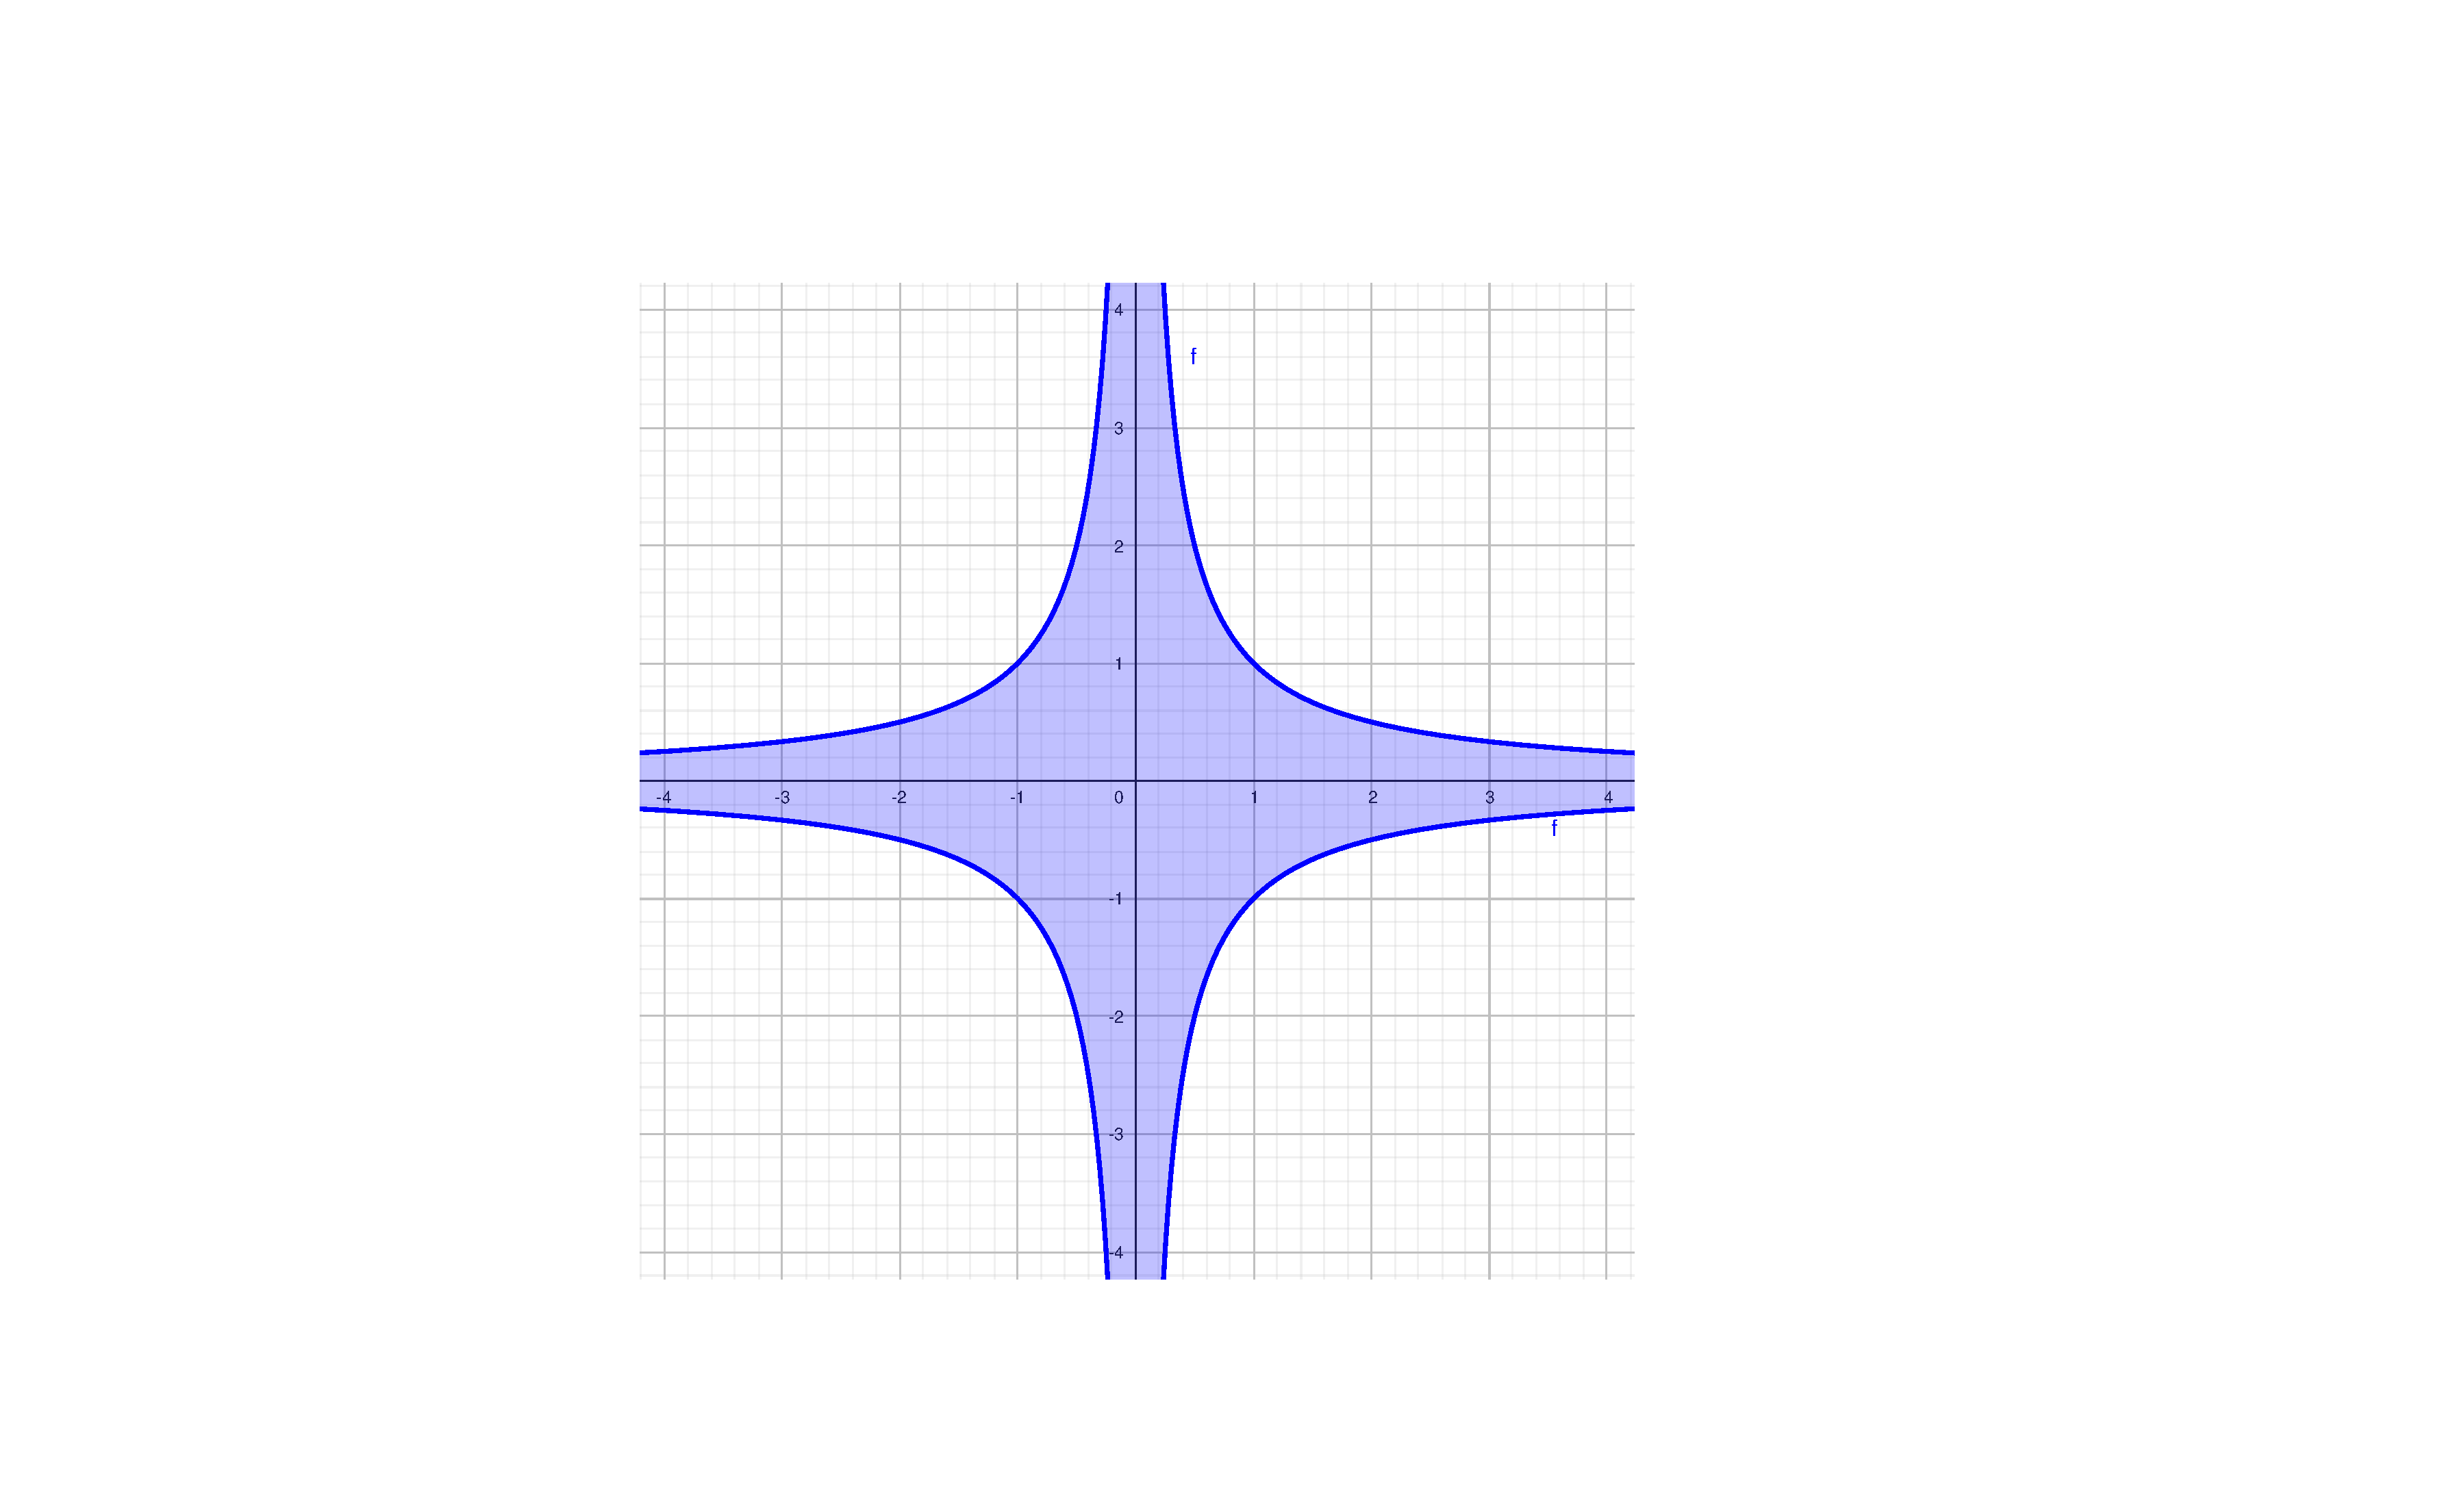
\includegraphics[width=.7\textwidth]{img/dominio_di_funzioni-5.pdf}
	\end{figure}
	\begin{itemize}
		\item L'insieme dei punti interni:
		\begin{equation*}
			\mathrm{int}\left(D\right) = \mathring{D} = \left\{\left(x,y\right) \in \mathbb{R}^{2} \: : \: -1 < xy < 1\right\}
		\end{equation*}

		\item L'insieme dei punti di frontiera:
		\begin{equation*}
			\partial D = \left\{\left(x,y\right) \in \mathbb{R}^{2} \: : \: -1 = xy \: \lor \: xy = 1\right\}
		\end{equation*}

		\item La chiusura:
		\begin{equation*}
			\overline{D} = D \cup \partial D = \left\{\left(x,y\right) \in \mathbb{R}^{2} \: : \: -1 \le xy \le 1\right\}
		\end{equation*}
	\end{itemize}
	L'insieme $D$ non è aperto poiché $D \ne \mathring{D}$ ma è chiuso poiché $D = \overline{D}$.\newpage

	\begin{flushleft}
		\example{\underline{Esempio 6}}
	\end{flushleft}

	\noindent
	Data la funzione:
	\begin{equation*}
		f\left(x,y\right) = \dfrac{\ln\left(1-x^{2}-y^{2}\right)}{\sqrt{x}}
	\end{equation*}
	Le condizioni d'esistenza sono sulla radice (maggiore di zero) e sul logaritmo (maggiore di zero):
	\begin{equation*}
		D = \left\{\left(x,y\right) \in \mathbb{R}^{2} \: : \: 1-x^{2}-y^{2} > 0 \: \land \: x > 0\right\}
	\end{equation*}
	Il dominio è rappresentabile accorgendosi che $1-x^{2}-y^{2}$ è una circonferenza con un'equazione canonica del tipo $x^{2} + y^{2} = 1$.
	\begin{figure}[!htp]
		\centering
		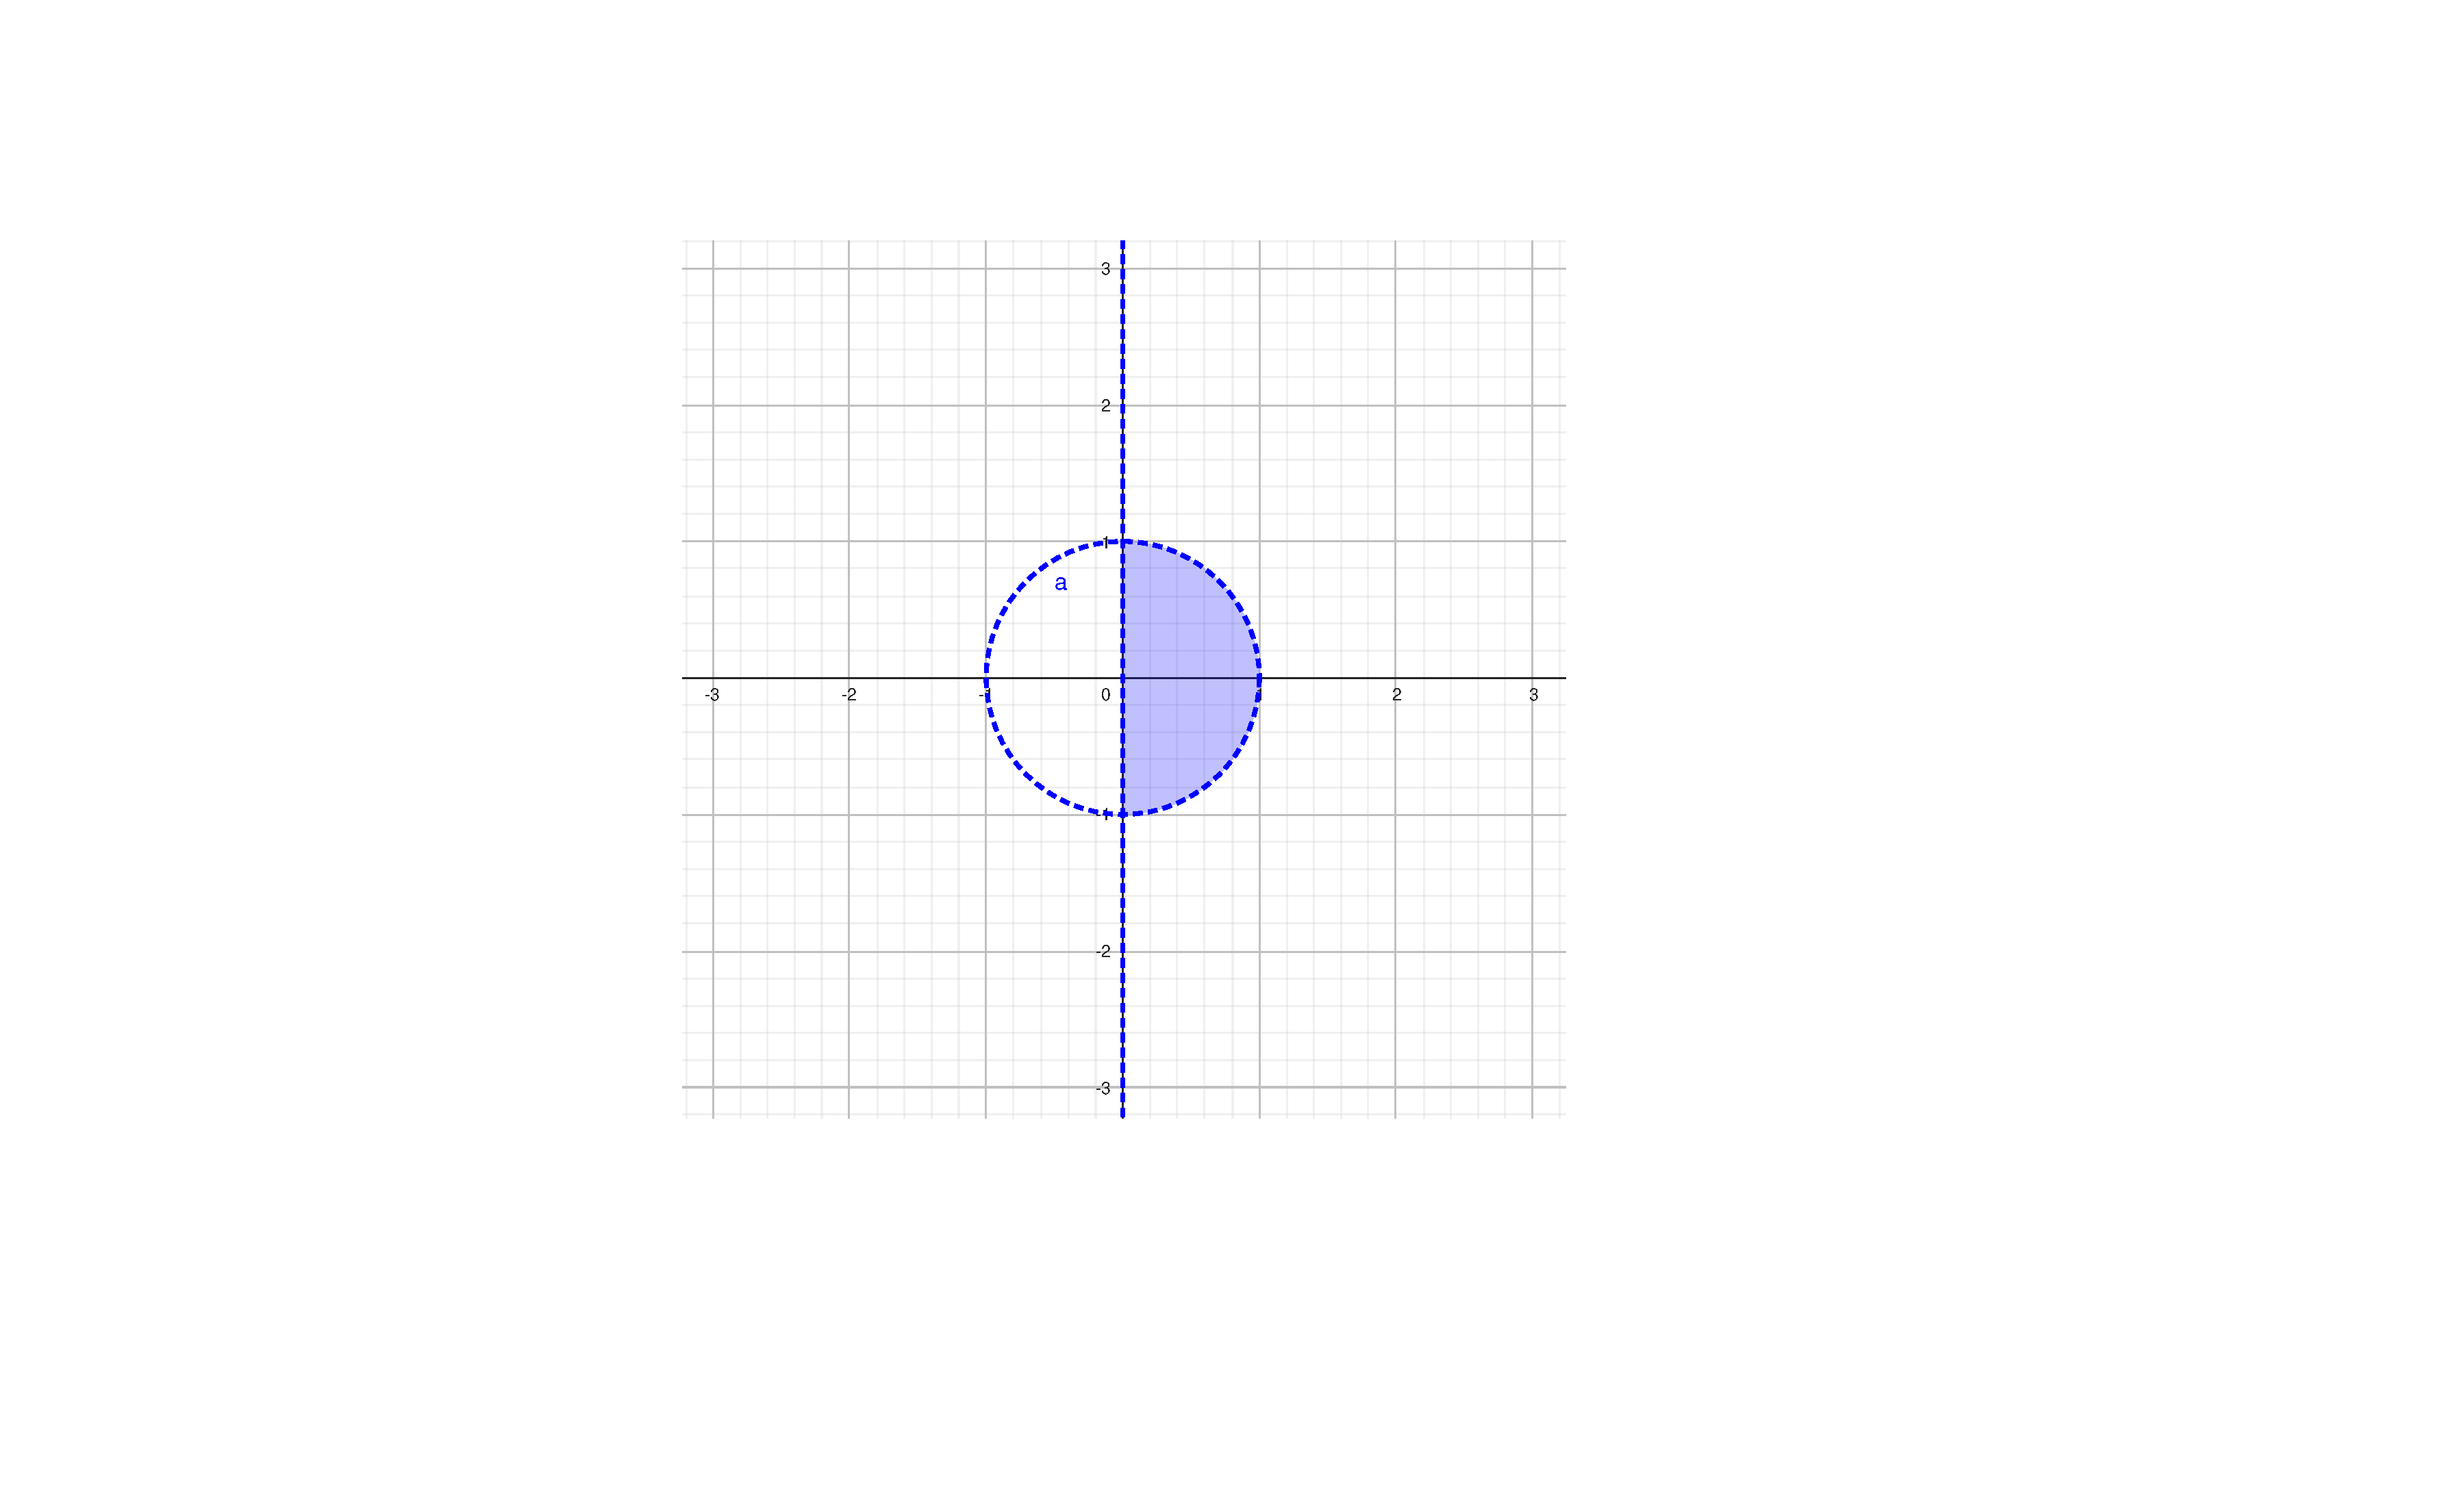
\includegraphics[width=.7\textwidth]{img/dominio_di_funzioni-6.pdf}
	\end{figure}
	\begin{itemize}
		\item L'insieme dei punti interni:
		\begin{equation*}
			\mathrm{int}\left(D\right) = \mathring{D} = \left\{\left(x,y\right) \in \mathbb{R}^{2} \: : \: 1-x^{2}-y^{2} > 0 \: \land \: x > 0\right\}
		\end{equation*}

		\item L'insieme dei punti di frontiera:
		\begin{equation*}
			\partial D = \left\{\left(x,y\right) \in \mathbb{R}^{2} \: : \: 1-x^{2}-y^{2} = 0 \: \land \: x = 0\right\}
		\end{equation*}

		\item La chiusura:
		\begin{equation*}
			\overline{D} = D \cup \partial D = \left\{\left(x,y\right) \in \mathbb{R}^{2} \: : \: 1-x^{2}-y^{2} \ge 0 \: \land \: x \ge 0\right\}
		\end{equation*}
	\end{itemize}
	L'insieme $D$ è aperto poiché $D = \mathring{D}$ ma non è chiuso poiché $D \ne \overline{D}$.\newpage

	\begin{flushleft}
		\example{\underline{Esempio 7}}
	\end{flushleft}

	\noindent
	Data la funzione:
	\begin{equation*}
		f\left(x,y,z\right) = \dfrac{1}{y^{2} + z^{2} - 4}
	\end{equation*}
	Sotto radice il valore deve essere diverso da zero, per cui $y^{2} + z^{2} - 4 \ne 0$. È possibile fare alcune manipolazioni $y^{2} + z^{2} \ne 4$ e scrivere il dominio come:
	\begin{equation*}
		D = \left\{\left(x,y,z\right) \in \mathbb{R}^{3} \: : \: y^{2} + z^{2} \ne 4\right\}
	\end{equation*}
	\begin{figure}[!htp]
		\centering
		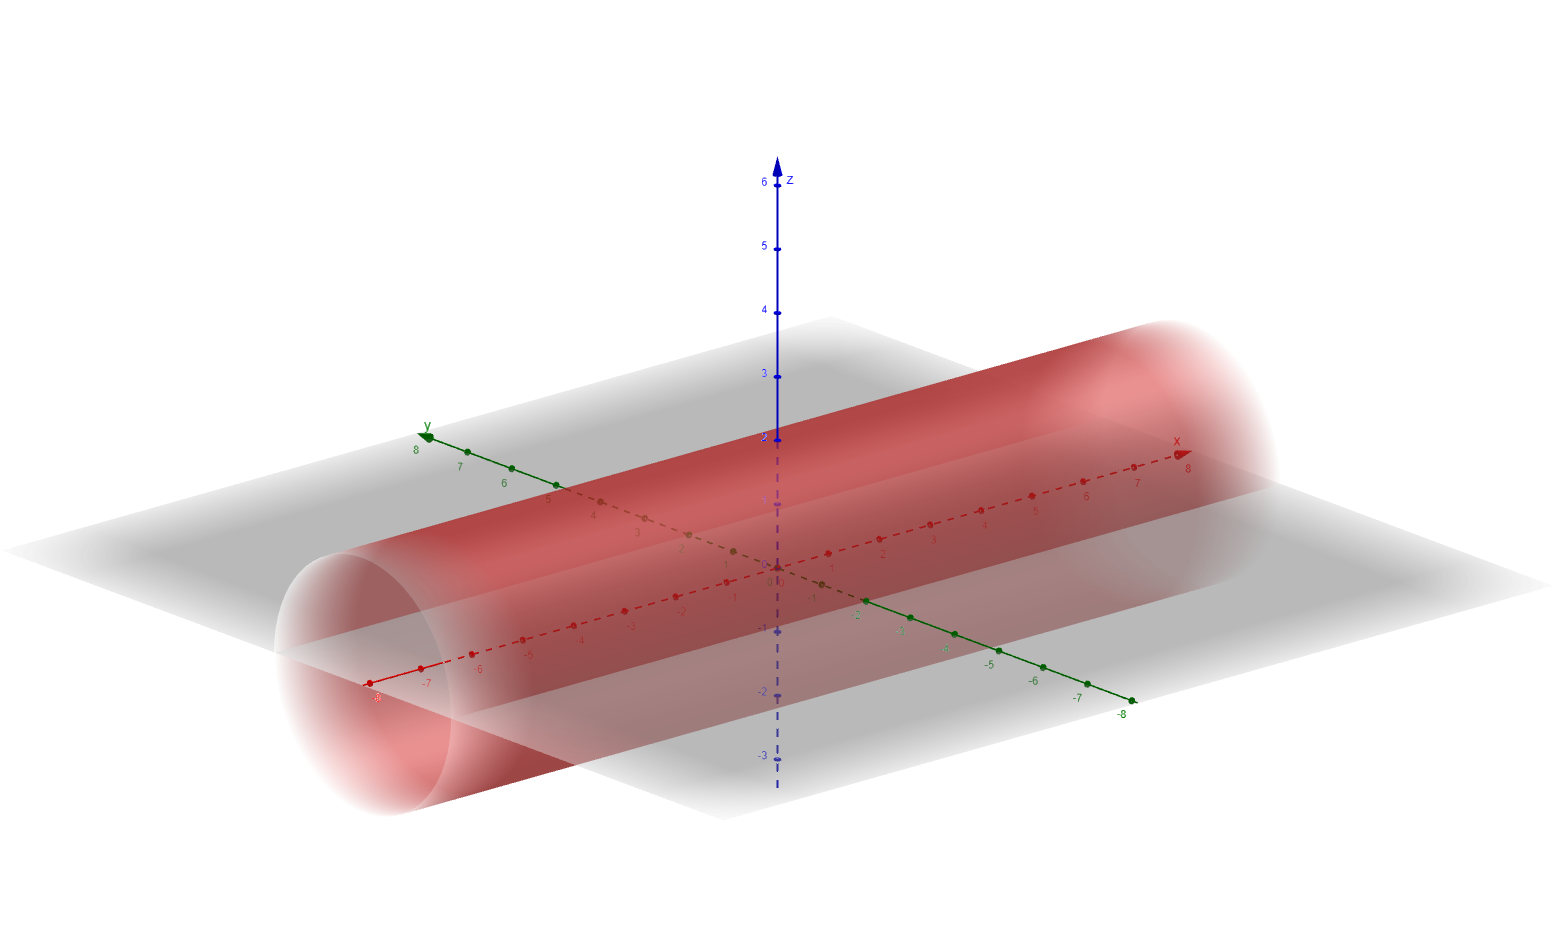
\includegraphics[width=\textwidth]{img/dominio_di_funzioni-7.png}
		\caption*{La linea blu è l'asse $z$ (intersecata in $\pm 2$), la linea verde è l'asse $y$ (intersecata in $\pm 2$), la linea rossa è l'asse $x$ (all'interno del cilindro).}
	\end{figure}
	\begin{itemize}
		\item L'insieme dei punti interni:
		\begin{equation*}
			\mathrm{int}\left(D\right) = \mathring{D} = \left\{\left(x,y,z\right) \in \mathbb{R}^{3} \: : \: y^{2} + z^{2} \ne 4 \right\}
		\end{equation*}

		\item L'insieme dei punti di frontiera:
		\begin{equation*}
			\partial D = \left\{\left(x,y,z\right) \in \mathbb{R}^{3} \: : \: y^{2} + z^{2} = 4\right\}
		\end{equation*}

		\item La chiusura:
		\begin{equation*}
			\overline{D} = D \cup \partial D = \text{non possibile}
		\end{equation*}
	\end{itemize}
	L'insieme $D$ è aperto poiché $D = \mathring{D}$ ma non è chiuso poiché $D \ne \overline{D}$.\newpage

	\begin{flushleft}\label{esempio bonus rappresentare un dominio}
		\example{\underline{Esempio bonus}}
	\end{flushleft}
	Data la funzione:
	\begin{equation*}
		f\left(x,y\right) = \ln\left(x^{2}-y^{2}+1\right) - \dfrac{1}{\sqrt{x}}
	\end{equation*}
	Il dominio è influenzato dal logaritmo e dalla radice al denominatore (combinazione di condizioni):
	\begin{equation*}
		D = \left\{\left(x,y\right) \in \mathbb{R}^{2} \: : \: x^{2} - y^{2} + 1 > 0 \: \land \: x > 0\right\}
	\end{equation*}
	L'equazione $x^{2} - y^{2} + 1$ è un'iperbole (par. \ref{subsubsection: iperbole}). Infatti basta ricordare che se $x^{2}$ e $y^{2}$ hanno segno concorde, allora si tratta di un'ellisse o di una circonferenza, mentre nel caso di segno discorde, si tratta di un'iperbole. Per rappresentarla, si eseguono alcune operazioni algebriche:
	\begin{equation*}
		x^{2} - y^{2} + 1 \rightarrow x^{2} - y^{2} = - 1
	\end{equation*}
	Si scrive l'equazione canonica:
	\begin{equation*}
		\begin{array}{rcl}
			\dfrac{\left(x-x_{C}\right)^{2}}{a^{2}} - \dfrac{\left(y-y_{C}\right)^{2}}{b^{2}} &=& \pm 1 \hspace{1.5em} \text{con } a \ne 0, \: b \ne 0 \\ [1em]
			%
			\dfrac{\left(x-0\right)^{2}}{1^{2}} - \dfrac{\left(y-0\right)^{2}}{1^{2}} &=& -1
		\end{array}
	\end{equation*}
	Per cui, l'iperbole ha centro nell'origine (lo si capisce dai $-0$!), il segno dell'$1$ è negativo, per cui l'iperbole ha un'intersezione nell'asse delle ordinate ($y$).

	\newpage

	\subsubsection{Grafico di una funzione scalare in \texorpdfstring{$n$}{n} variabili}\label{subsubsection: grafico di una funzione scalare in n variabili}

	\begin{boxdef}
		Se $f$ è una funzione reale di due variabili reali con dominio $D$, il \definition{grafico} della funzione $f$ è l'insieme di tutti i punti $\left(x,y,z\right) \in \mathbb{R}^{3}$ tali che $z = f\left(x,y\right)$, con $\left(x,y\right) \in D$.
	\end{boxdef}
	
	\noindent
	La definizione si può estendere per $n > 2$. In altre parole, il grafico di una funzione è:
	\begin{equation*}
		\Gamma\left(f\right) = \left\{\left(x, f\left(x\right)\right) \in \mathbb{R}^{n+1}\right\}
	\end{equation*}
	Nel caso di $n = 2$, il grafico della funzione $f$ risulta:
	\begin{figure}[!htp]
		\centering
		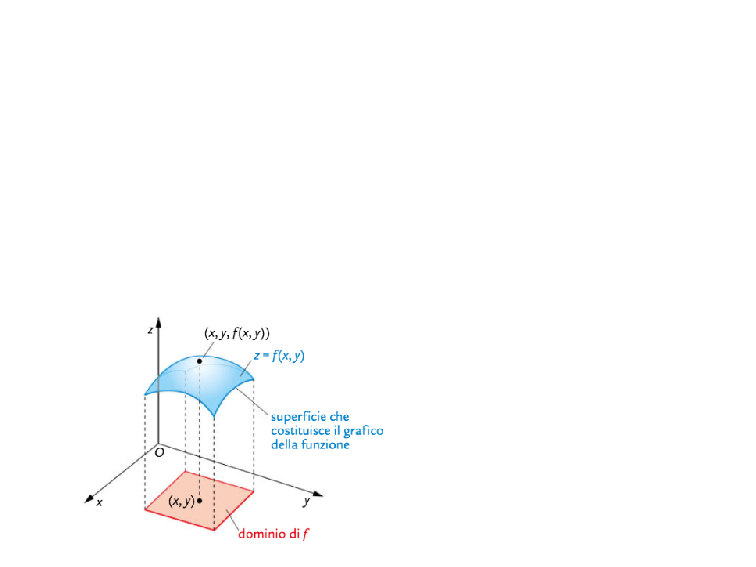
\includegraphics[width=.5\textwidth]{img/grafico_di_una_funzione.pdf}
	\end{figure}

	\longline

	\subsubsection{Esempio di grafico di funzioni a due variabili}\label{subsubsection: esempi di grafico di funzioni a due variabili}

	Data la funzione:
	\begin{equation*}
		f\left(x,y\right) = \sqrt{9 - x^{2} - y^{2}}
	\end{equation*}
	La sua condizione d'esistenza è determinata dalla radice quadrata:
	\begin{equation*}
		D = \left\{\left(x,y\right) \in \mathbb{R}^{2} \: : \: 9 - x^{2} - y^{2} \ge 0 \right\}
	\end{equation*}
	Il dominio è una circonferenza di raggio $3$ ($\sqrt{9}$):\newpage
	\begin{figure}[!htp]
		\centering
		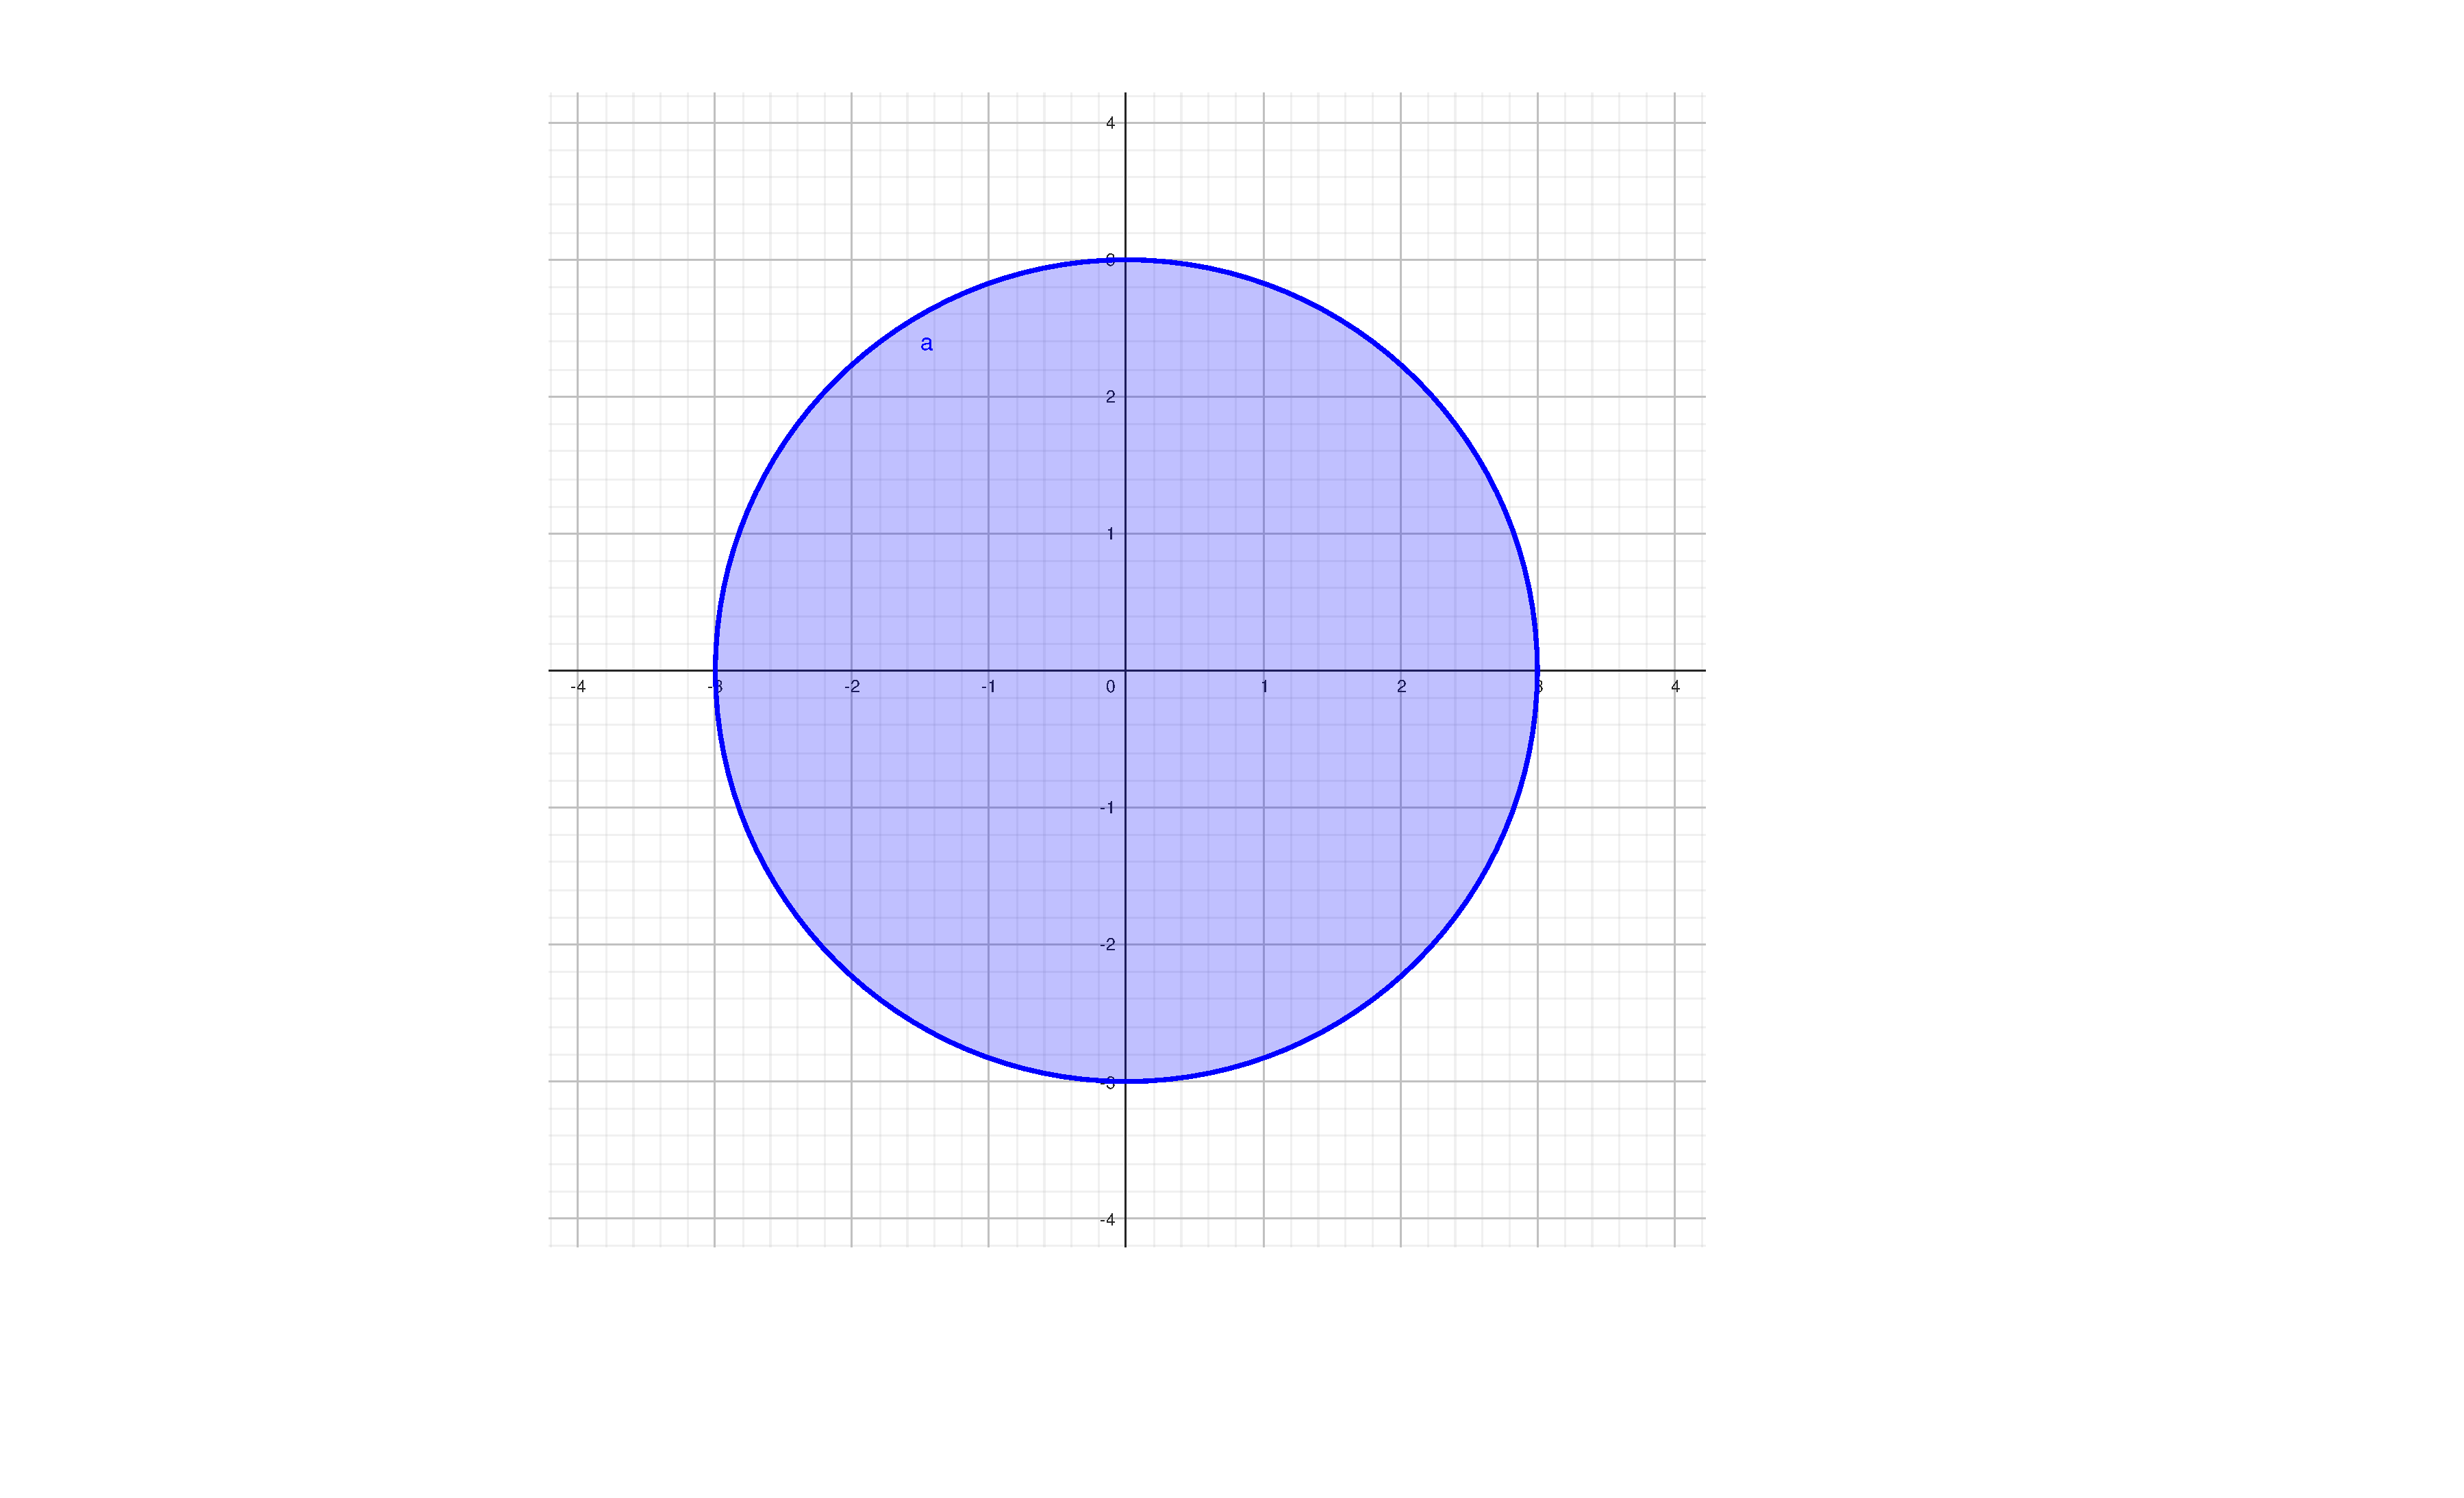
\includegraphics[width=.5\textwidth]{img/grafico_di_funzioni-1.pdf}
	\end{figure}

	\noindent
	Invece, per quanto riguarda il grafico della funzione, si applica la formula. Per cui, il grafico avrà il seguente dominio:
	\begin{equation*}
		\Gamma\left(f\right) = \left\{\left(x,y,z\right) \in \mathbb{R}^{3} \: : \: z = f\left(x,y\right)\right\} = \left\{\left(x,y,z\right) \in \mathbb{R}^{3} \: : \: z = \sqrt{9 - x^{2} - y^{2}}\right\}
	\end{equation*}
	Per rappresentare la figura, si deve avere un po' di intuito poiché è noto che una sfera abbia i termini $x,y,z$ al quadrato. Di conseguenza, la $z$ può essere anche vista come $x^{2} = 9 - x^{2} - y^{2}$. E con alcuni aggiustamenti aritmetici, si giunge all'equazione canonica $x^{2} + y^{2} + z^{2} = 9$. Il dominio del grafico può essere riscritto ricordandosi di aggiungere la condizione d'esistenza sulla $z$, cioè il maggiore uguale dovuto alla radice quadrata.
	\begin{equation*}
		\Gamma\left(f\right) = \left\{\left(x,y,z\right) \in \mathbb{R}^{3} \: : \: z \ge 0, \: x^{2} + y^{2} + z^{2} = 9 \right\}
	\end{equation*}
	Il grafico è una sfera tagliata a metà a causa della $z \ge 0$:
	\begin{figure}[!htp]
		\centering
		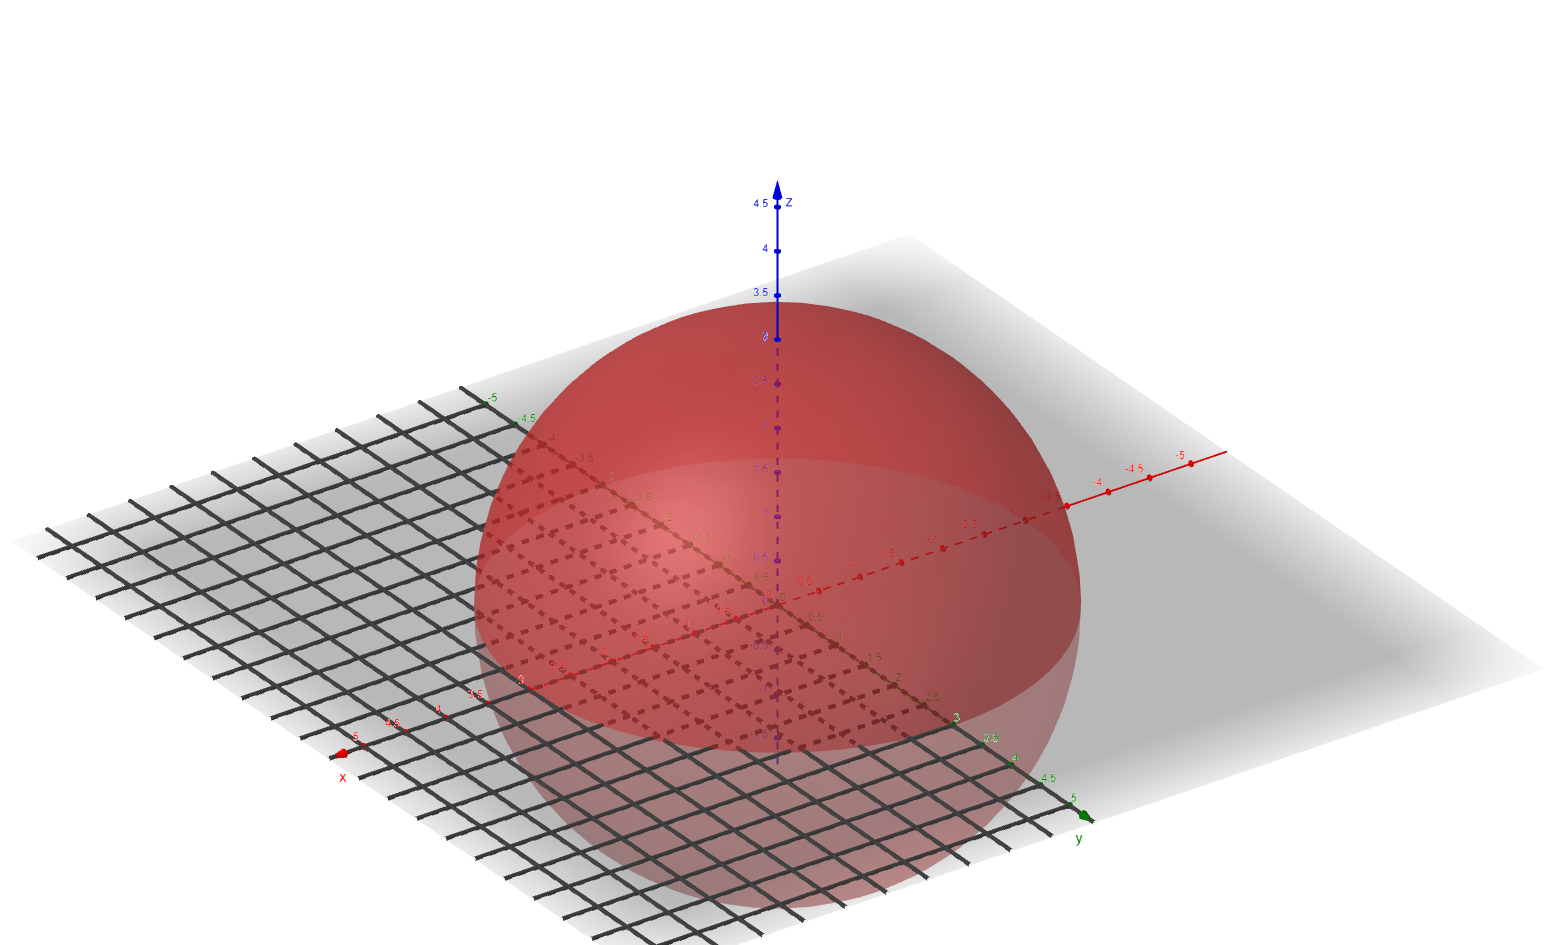
\includegraphics[width=\textwidth]{img/grafico_di_una_funzione.png}
	\end{figure}\newpage

	\subsection{Insiemi (curve) di livello}\label{subsection: insiemi (curve) di livello}

	L'insieme dei punti nel dominio di una funzione $f$ che hanno la stessa immagine $k \in \mathbb{R}$ si chiama \definition{insieme di livello} $k$ (o curve di livello):
	\begin{equation}\label{eq: curve di livello}
		L_{k}\left(f\right) = \left\{x \in \mathbb{R}^{n} \: : \: f\left(x\right) = k\right\}
	\end{equation}
	Nel caso in cui $n = 2$, la funzione $L_{k}\left(f\right)$ è la proiezione sul piano $xy$ della curva che si ottiene intersecando il grafico della funzione $f$ con il piano $z = k$.\newline

	\noindent
	In parole povere, le \definition{curve di livello} forniscono una rappresentazione bidimensionale del grafico della funzione $f$. Questo rendere la rappresentazione, talvolta, più chiara e semplice da eseguire.\newpage

	\subsubsection{Alcuni esempi}\label{subsubsection: alcuni esempi}

	\begin{flushleft}
		\example{\underline{Esempio 1}}
	\end{flushleft}
	Data la funzione:
	\begin{equation*}
		f\left(x,y\right) = \sqrt{9-x^{2} -y^{2}}
	\end{equation*}
	E il dominio relativo (già calcolato nel par. \ref{subsubsection: esempi di grafico di funzioni a due variabili}):
	\begin{equation*}
		D = \left\{\left(x,y\right) \in \mathbb{R}^{2} \: : \: 9 - x^{2} - y^{2} \ge 0 \right\}
	\end{equation*}
	La funzione è una circonferenza di raggio $3$. Di conseguenza, le curve di livello andranno da un massimo di raggio pari a $3$ ad un minimo pari a $0$:
	\begin{figure}[!htp]
		\centering
		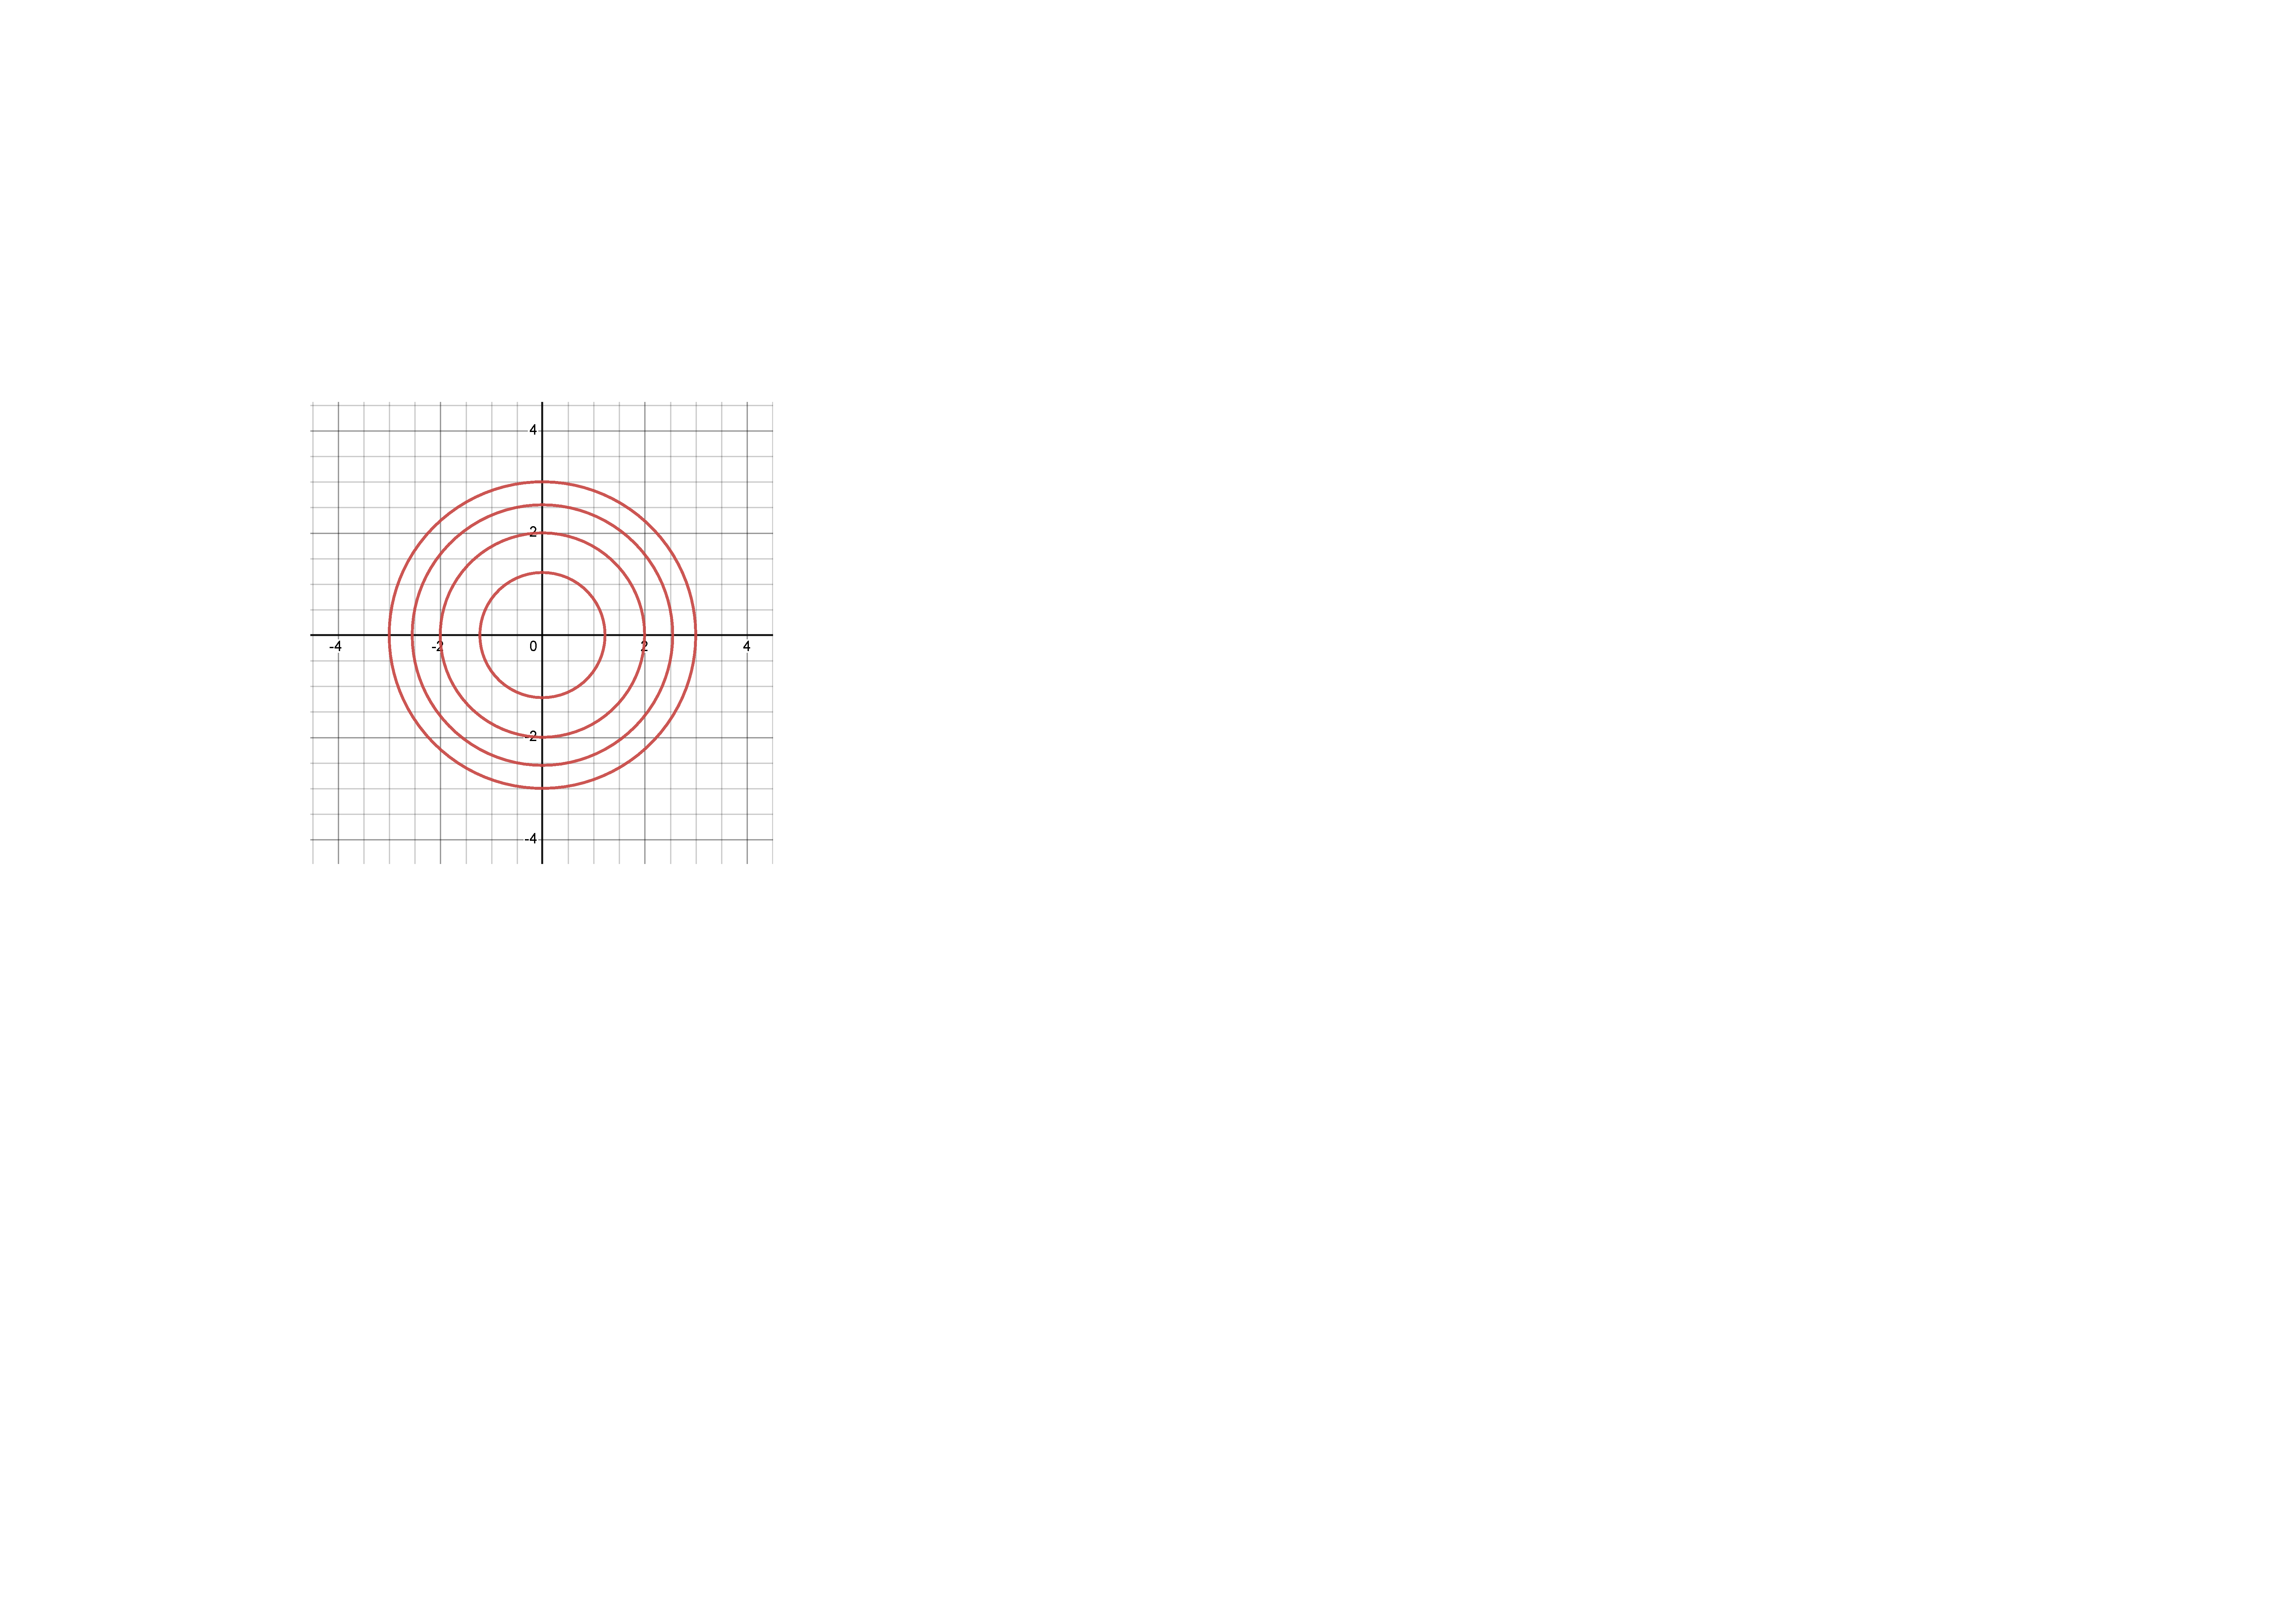
\includegraphics[width=.65\textwidth]{img/curve_di_livello-1.pdf}
	\end{figure}
	
	\noindent
	In forma matematica (eq. \ref{eq: curve di livello}):
	\begin{equation*}
		L_{k}\left(f\right) = \left\{\left(x,y\right) \in \mathbb{R}^{2} \: : \: f\left(x,y\right) = k\right\} = \left\{\left(x,y\right) \in \mathbb{R}^{2} \: : \: \sqrt{9-x^{2} -y^{2}} = k\right\}
	\end{equation*}
	Per rappresentarla facilmente, si utilizzano alcune manipolazioni algebriche:
	\begin{equation*}
		\begin{array}{rcl}
			\sqrt{9-x^{2} -y^{2}} &=& k \\ [.3em]
			9-x^{2} -y^{2} &=& k^{2} \\ [.3em]
			-x^{2} -y^{2} &=& k^{2} - 9 \\ [.3em]
			x^{2} + y^{2} &=& 9 - k^{2}
		\end{array}
	\end{equation*}
	Risulta evidente adesso che modificando la $k$, si modifica il raggio della circonferenza ($x^{2}+y^{2}$). Per cui, è immediato il fatto che la $k$ debba essere compresa tra $0$ e $3$:
	\begin{equation*}
		0 \le k \le 3
	\end{equation*}
	Infatti, nel grafico delle curve di livello nella pagina precedente, la seconda curva di livello interseca il valore $2$. Questo perché con $k = \sqrt{5}$ si ha:
	\begin{equation*}
		L_{\sqrt{5}}\left(f\right) = \left\{\left(x,y\right) \in \mathbb{R}^{2} \: : \: x^{2} + y^{2} = 9 - \left(\sqrt{5}\right)^{2} \Rightarrow x^{2} + y^{2} = 4\right\}
	\end{equation*}\newpage

	\begin{flushleft}
		\example{\underline{Esempio 2}}
	\end{flushleft}
	Data la funzione:
	\begin{equation*}
		f\left(x,y\right) = e^{-x^{2}-y^{2}}
	\end{equation*}
	E il dominio risulta essere:
	\begin{equation*}
		D = \left\{\left(x,y\right) \in \mathbb{R}^{2} \: : \: \mathbb{R}^{2}\right\}
	\end{equation*}
	Si applicano le curve di livello, utilizzando sempre l'equazione \ref{eq: curve di livello}:
	\begin{equation*}
		L_{k}\left(f\right) = \left\{\left(x,y\right) \in \mathbb{R}^{2} \: : \: e^{-x^{2}-y^{2} = k}\right\}
	\end{equation*}
	L'espressione è possibile riscriverla come:
	\begin{equation*}
		-x^{2}-y^{2} = \ln\left(k\right) \rightarrow x^{2} + y^{2} = -\ln\left(k\right)
	\end{equation*}
	Dalla quale si ricava la condizione d'esistenza $k > 0$. Si deduce che se $k \le 0$, le curve di livello hanno valore $0$:
	\begin{equation*}
		\begin{cases}
			L_{k} = 0 & k \le 0 \\
			L_{k} = \left\{\left(x,y\right) \in \mathbb{R}^{2} \: : \: x^{2}+y^{2} = -\ln\left(k\right)\right\} & k > 0
		\end{cases}
	\end{equation*}
	Ma non solo, nel caso in cui $k > 0$, la condizione è rispettata finché il risultato del logaritmo è negativo o uguale a zero. Con $k = 1$ il logaritmo si annulla e la condizione $x^{2} + y^{2} = 0$ è rispettata. Ma con $k = 2$ il risultato è $\approx - 0.69$ e la condizione non viene rispettata. Di conseguenza, si aggiorna il sistema:
	\begin{equation*}
		\begin{cases}
			L_{k} = 0 & k \le 0 \\
			L_{k} = \left\{\left(x,y\right) \in \mathbb{R}^{2} \: : \: x^{2}+y^{2} = -\ln\left(k\right)\right\} & 0 < k \le 1 \\
			\uparrow & \text{otherwise}
		\end{cases}
	\end{equation*}\newpage

	\begin{flushleft}
		\example{\underline{Esempio 3}}
	\end{flushleft}
	Data la funzione:
	\begin{equation*}
		f\left(x,y\right) = \sqrt{11 - 4x^{2} - 9y^{2} + 16x - 18y}
	\end{equation*}
	Il dominio è semplicemente maggiore o uguale a zero:
	\begin{equation*}
		D = \left\{\left(x,y\right) \in \mathbb{R}^{2} \: : \: 11 - 4x^{2} - 9y^{2} + 16x - 18y \ge 0\right\}
	\end{equation*}
	Con qualche manipolazione algebrica, per ottenere l'equazione canonica, si ottiene:
	\begin{equation*}
		4x^{2} + 9y^{2} - 16x + 18y - 11 \le 0
	\end{equation*}
	Prima di tracciare le curve di livello è necessario rappresentare il dominio. Quindi, si sceglie di rappresentarlo alla frontiera, ovvero sia:
	\begin{equation*}
		4x^{2} + 9y^{2} - 16x + 18y = 11
	\end{equation*}
	Per convincersi che sia la frontiera, basta considerare la disuguaglianza del dominio:
	\begin{equation*}
		4x^{2} + 9y^{2} - 16x + 18y - 11 \le 0 \: \rightarrow \: 4x^{2} + 9y^{2} - 16x + 18y \le 11
	\end{equation*}
	Risulta evidente che i valori di sinistra devono essere minore o al massimo uguale a $11$.\newline

	\noindent
	Per rappresentare l'ellisse, è necessario ottenere l'equazione canonica. Quindi, si eseguono alcune manipolazioni algebriche:
	\begin{equation*}
		\begin{array}{rcl}
			4x^{2} + 9y^{2} - 16x + 18y &=& 11 \\ [.3em]
			4\left(x^{2} - 4x\right) + 9\left(y^{2} + 2y\right) &=& 11
		\end{array}
	\end{equation*}
	Dal paragrafo \ref{subsubsection: ellisse} si ricorda che l'equazione canonica è nella forma:
	\begin{equation*}
		\dfrac{\left(x-x_{C}\right)^{2}}{a^{2}} + \dfrac{\left(y-y_{C}\right)^{2}}{b^{2}} = 1
	\end{equation*}
	Per cui come è possibile procedere? Ci viene in soccorso il completamento dei quadrati (par. \ref{subsubsection: completamento dei quadrati}):
	\begin{enumerate}[label=\alph*.]
		\item Si cerca un $\Delta$ per ogni equazione di secondo grado (per $x$ e per $y$) tale che sia uguale a zero:
		\begin{equation*}
			\begin{array}{rcl}
				4x^{2} + 9y^{2} - 16x + 18y &=& 11 \\ [.3em]
				4x^{2} - 16x + 9y^{2} + 18y &=& 11 \\ [1em]
				%%
				4x^{2} - 16x &\rightarrow& \left(-16\right)^{2} - 4 \cdot 4 \cdot c = 0 \\ [.3em]
				&& -16c = -\left(-16\right)^{2} \\ [.3em]
				&& c = 16 \\ [1em]
				%%
				9y^{2} + 18y &\rightarrow& \left(18\right)^{2} - 4 \cdot 9 \cdot c = 0 \\ [.3em]
				&& -36c = -324 \\ [.3em]
				&& c = 9
			\end{array}
		\end{equation*}

		\item Si riscrive l'equazione con i nuovi termini ma lasciandola invariata, per cui:
		\begin{equation*}
			\begin{array}{rcl}
				\left(4x^{2} - 16x\right) + \left(9y^{2} + 18y\right) &=& 11 \\ [.3em]
				\left(4x^{2} - 16x + 16 - 16\right) + \left(9y^{2} + 18y + 9 - 9\right) &=& 11
			\end{array}
		\end{equation*}
		
		\item Si resiste alla voglia di semplificare e si esegue un raggruppamento:
		\begin{equation*}
			\begin{array}{rcl}
				4x^{2} - 16x + 16 &\rightarrow& 4\left(x^{2} - 4x + 4\right) \\ [.3em]
											 && 4\left(x-2\right)^{2} \\ [1em]
				9y^{2} + 18y + 9  &\rightarrow& 9\left(y^{2} + 2y + 1\right) \\ [.3em]
											 && 9\left(y+1\right)^{2}
			\end{array}
		\end{equation*}
		Per raggruppare in questo modo basta calcolare trovare le soluzioni dell'equazione di secondo grado e riscriverle come quadrato. Quindi, data l'equazione di secondo grado $ax^{2}+bx+c$:
		\begin{equation*}
			\dfrac{-b \pm \sqrt{b^{2} - 4 \cdot a \cdot c}}{2 \cdot a} \: \xRightarrow{\Delta = 0} \: \dfrac{-b}{2a} = \lambda \: \rightarrow \: \left(x-\lambda\right)^{2}
		\end{equation*}
		E infatti sostituendo l'equazione $x^{2} - 4x + 4$:
		\begin{equation*}
			\dfrac{-\left(-4\right) \pm \sqrt{\left(-4\right)^{2} - 4 \cdot 1 \cdot 4}}{2 \cdot 1} \: \xRightarrow{\Delta = 0} \: \dfrac{4}{2} = 2 \: \rightarrow \: \left(x-2\right)^{2}
		\end{equation*}

		\item Si riscrive l'equazione dopo il raggruppamento:
		\begin{equation*}
			\left(4\left(x-2\right)^{2} - 16\right) + \left(9\left(y+1\right)^{2} - 9\right) = 11
		\end{equation*}
		A questo punto si possono portare a destra i termini non legati alle variabili $x$ e $y$:
		\begin{equation*}
			4\left(x-2\right)^{2} + 9\left(y+1\right)^{2} = 36
		\end{equation*}

		\item A destra è necessario il valore $1$ per l'equazione canonica, dunque viene in automatico dividere tutto per $36$:
		\begin{equation*}
			\begin{array}{rcl}
				\dfrac{1}{36} \cdot 4\left(x-2\right)^{2} + \dfrac{1}{36} \cdot 9\left(y+1\right)^{2} &=& 36 \cdot \dfrac{1}{36} \\ [1em]
				\dfrac{\left(x-2\right)^{2}}{9} + \dfrac{\left(y+1\right)^{2}}{4} &=& 1
			\end{array}
		\end{equation*}
	\end{enumerate}
	Dato che il centro dell'ellisse è dato dai valori che vengono sottratti a $x^{2}$ ($x^{2}-x_{C}$) e $y^{2}$ ($y^{2}-y_{C}$), in questo caso le coordinate sono: $\left(2, -1\right)$. I vertici sono piuttosto immediati:
	\begin{equation*}
		\begin{array}{lclclcl}
			\text{Vertice sx} &\rightarrow& \left(2-\sqrt{9}, -1\right) && \text{Vertice dx} &\rightarrow& \left(2+\sqrt{9}, -1\right) \\ [.3em]
										 && \left(-1, -1\right) && && \left(5, -1\right) \\ [.3em]
			\text{Vertice up} &\rightarrow& \left(2, -1 + \sqrt{4}\right) && \text{Vertice down} &\rightarrow& \left(2, -1-\sqrt{4}\right) \\ [.3em]
			&& \left(2, 1\right) && && \left(2, -3\right) \\
		\end{array}
	\end{equation*}\newpage

	\begin{figure}[!htp]
		\centering
		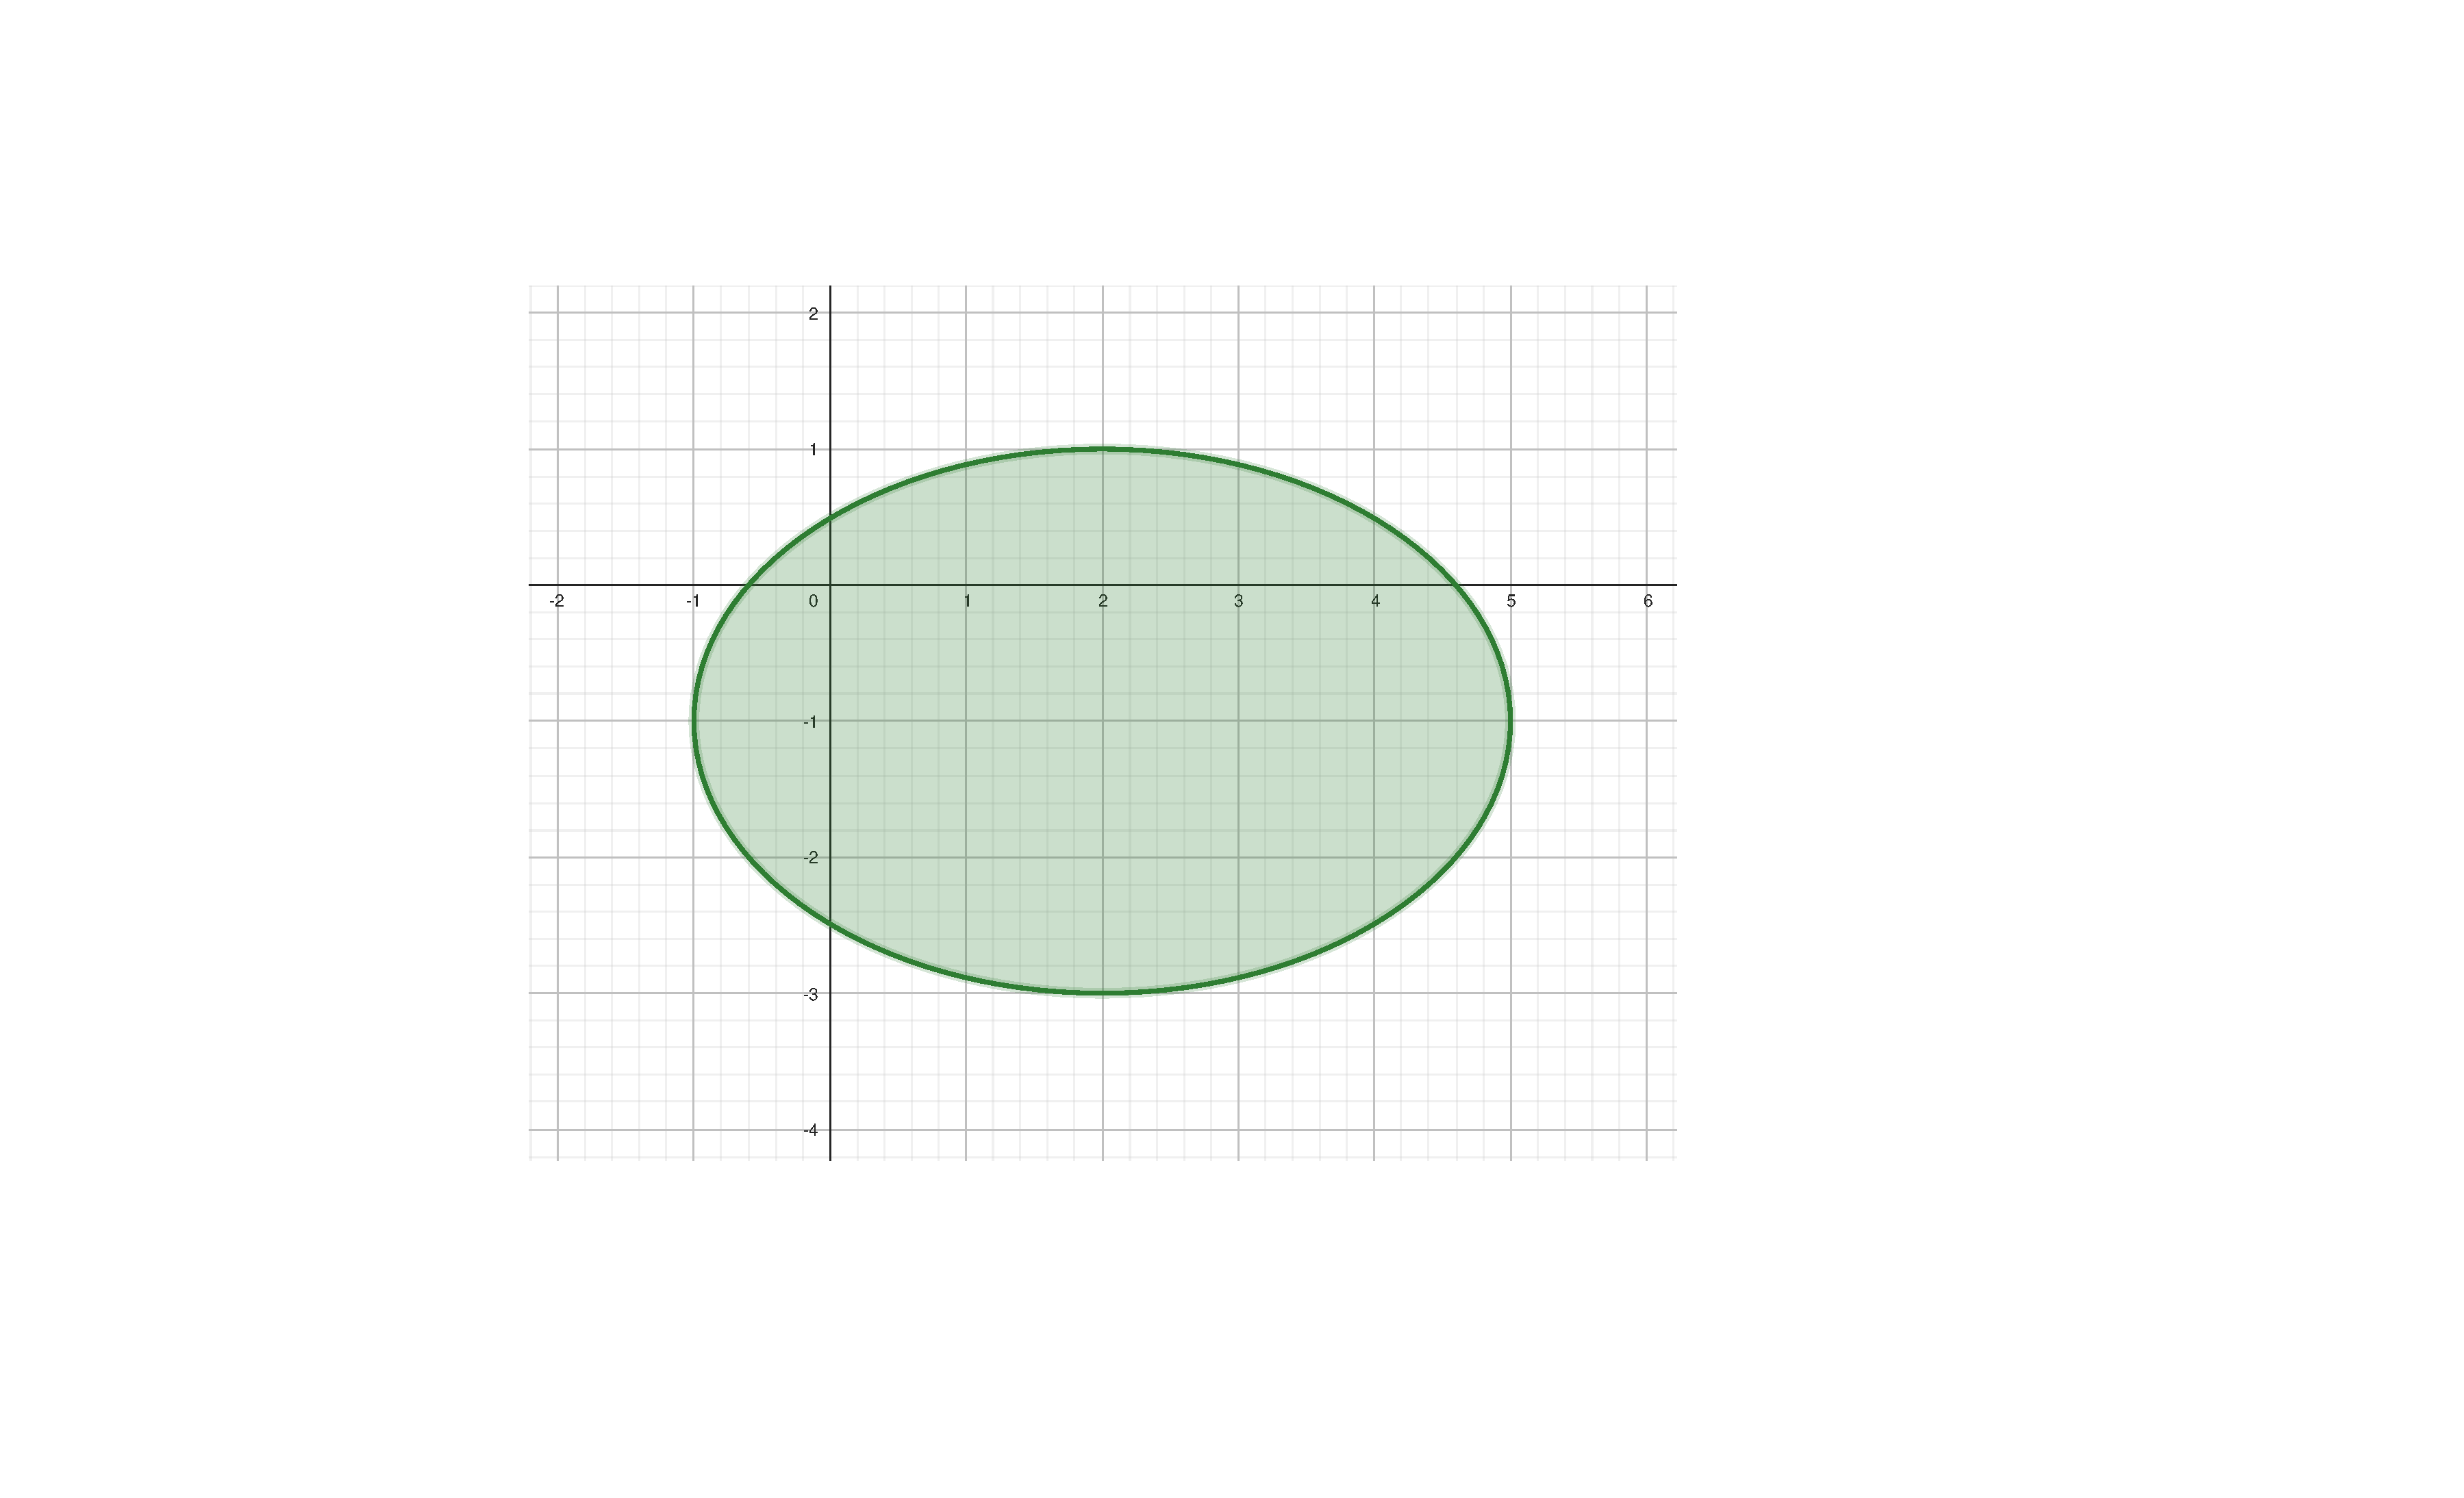
\includegraphics[width=.8\textwidth]{img/curve_di_livello-2.pdf}
		\caption*{La figura dell'ellisse alla frontiera e rappresenta anche la curva di livello più bassa poiché è al limite.}
	\end{figure}

	\noindent
	Il motivo per cui si dice "è al limite" è dato dal fatto che con $k$ sotto radice, la sua condizione d'esistenza è $k\ge 0$. Per cui, rappresentare:
	\begin{equation*}
		4x^{2}+9y^{2}-16x+18y-11 = 0
	\end{equation*}
	È identico a rappresentare:
	\begin{equation*}
		4x^{2}+9y^{2}-16x+18y-11 = \sqrt{k} \hspace{1em} \text{con } k = 0
	\end{equation*}
	Per completezza, si rappresenta una curva di livello utilizzando $k = \sqrt{11}$ e l'equazione \ref{eq: curve di livello} delle curve di livello:
	\begin{equation*}
		L_{\sqrt{11}}\left(f\right) = \left\{\left(x,y\right) \in \mathbb{R}^{2} \: : \: f\left(x,y\right) = \sqrt{11}\right\}
	\end{equation*}
	Per cui l'equazione da rappresentare è:
	\begin{equation*}
		\begin{array}{rcl}
			\sqrt{11 - 4x^{2} - 9y^{2} + 16x - 18y} &=& \sqrt{11} \\ [.3em]
			11 - 4x^{2} - 9y^{2} + 16x - 18y &=& 11 \\ [.3em]
			4x^{2} + 9y^{2} - 16x + 18y &=& 0
		\end{array}
	\end{equation*}
	Come in precedenza, si procede con il completamento dei quadrati:
	\begin{gather*}
		4x^{2} - 16x + 9y^{2} + 18y = 0 \\
		\downarrow \\
		\begin{array}{rcl}
			4x^{2} - 16x &\rightarrow& \left(-16\right)^{2} - 4 \cdot 4 \cdot c = 0 \\ [.3em]
									&& -16c = -\left(-16\right)^{2} \\ [.3em]
									&& c = 16 \\ [1em]
			9y^{2} + 18y &\rightarrow& \left(18\right)^{2} - 4 \cdot 9 \cdot c = 0 \\ [.3em]
									&& -36c = -324 \\ [.3em]
									&& c = 9
		\end{array}
	\end{gather*}
	\begin{gather*}
		\downarrow \\
		\left(4x^{2} - 16x + 16 - 16\right) + \left(9y^{2} + 18y + 9 - 9\right) = 0 \\
		\downarrow \\
		\begin{array}{rcl}
			4x^{2} - 16x + 16 &\rightarrow& 4\left(x^{2} - 4x + 4\right) \\ [.3em]
										 && 4\left(x-2\right)^{2} \\ [1em]
			9y^{2} + 18y + 9  &\rightarrow& 9\left(y^{2} + 2y + 1\right) \\ [.3em]
										 && 9\left(y+1\right)^{2}
		\end{array} \\
		\downarrow \\
		4\left(x-2\right)^{2} - 16 + 9\left(y+1\right)^{2} - 9 = 0 \\
		4\left(x-2\right)^{2} + 9\left(y+1\right)^{2} = 25 \\
		\downarrow \\
		\begin{array}{rcl}
			\dfrac{1}{25} \cdot 4\left(x-2\right)^{2} + \dfrac{1}{25} \cdot 9\left(y+1\right)^{2} &=& 25 \cdot \dfrac{1}{25} \\ [1em]
			\dfrac{\left(x-2\right)^{2}}{\frac{25}{4}} + \dfrac{\left(y+1\right)^{2}}{\frac{25}{9}} &=& 1
		\end{array}
	\end{gather*}
	Il centro dell'ellisse è $\left(2, -1\right)$ e i vertici sono:
	\begin{equation*}
		\begin{array}{lclclcl}
			\text{Vertice sx} &\rightarrow& \left(2-\sqrt{\frac{25}{4}}, -1\right) && \text{Vertice dx} &\rightarrow& \left(2+\sqrt{\frac{25}{4}}, -1\right) \\ [.8em]
										 && \left(-\frac{1}{2}, -1\right) && && \left(\frac{9}{2}, -1\right) \\ [.8em]
			\text{Vertice up} &\rightarrow& \left(2, -1 + \sqrt{\frac{25}{9}}\right) && \text{Vertice down} &\rightarrow& \left(2, -1-\sqrt{\frac{25}{9}}\right) \\ [.8em]
			&& \left(2, \frac{2}{3}\right) && && \left(2, -\frac{8}{3}\right)
		\end{array}
	\end{equation*}
	La figura dell'ellisse:
	\begin{figure}[!htp]
		\centering
		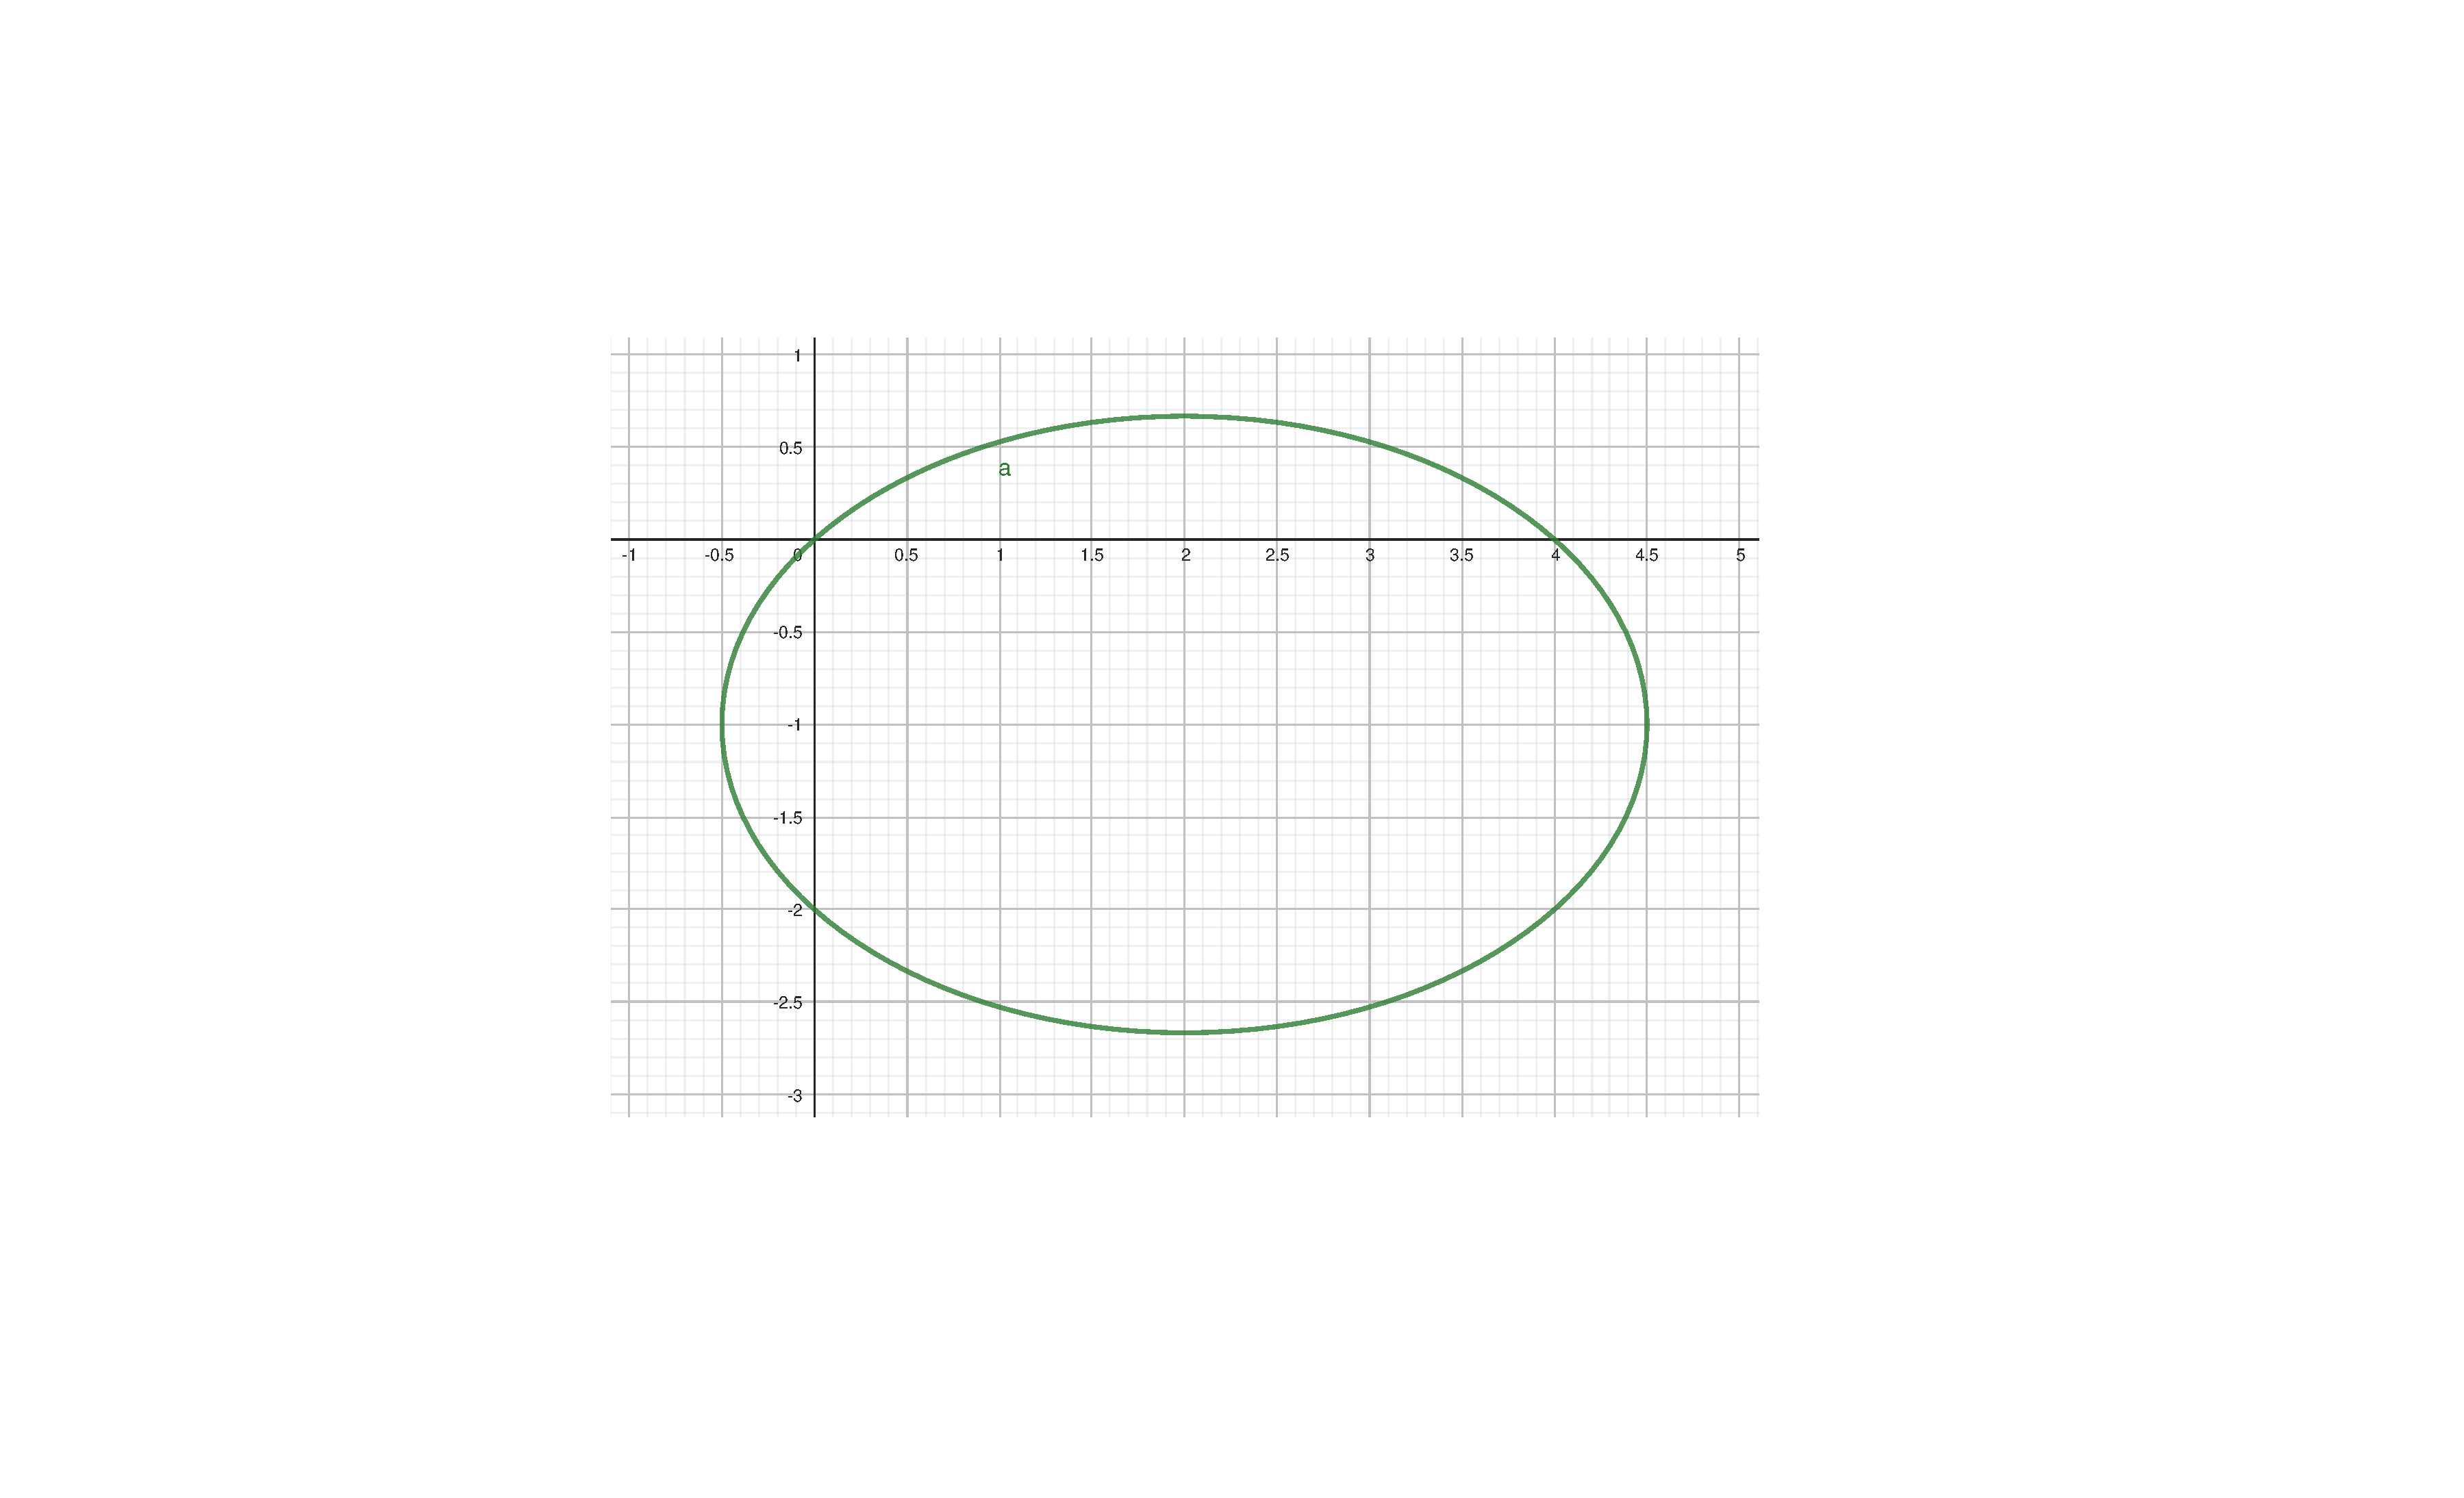
\includegraphics[width=.9\textwidth]{img/curve_di_livello-3.pdf}
	\end{figure}\newpage

	\subsection{Continuità}\label{subsection: continuità}

	Si mostra la definizione di continuità.

	\begin{boxdef}
		Si consideri una funzione $f \: : \: D \subseteq \mathbb{R}^{n} \rightarrow \mathbb{R}$ e un punto $x_{0} \in D$. La funzione $f$ è \definition{continua} nel punto $x_{0}$ se per ogni intorno $V$ di $f\left(x_{0}\right)$ esiste un intorno di $U$ di $x_{0}$ tale che:
		\begin{equation*}
			f\left(x\right) \in V \hspace{1.5em} \forall \: x \in U \cap D
		\end{equation*}
	\end{boxdef}

	\noindent
	Una \definition{notazione} utilizzata talvolta per dimostrare la continuità, è $\varepsilon - \delta$: per ogni $\varepsilon$ esiste un $\delta > 0$ tale che $\left| f\left(x\right) - f\left(x_{0}\right) \right| < \varepsilon$ per ogni $x$ appartenente a $D$ e dunque la distanza (par. \ref{subsection: spazio metrico e distanza}, eq. \ref{eq: distanza euclidea}) è minore di $\delta$ ($\left|\left| x - x_{0} \right|\right| < \delta$).\newline

	\framedtext{%
		\begin{flushleft}
			\example{\underline{Esempio}}
		\end{flushleft}
		
		Questo metodo è estendibile a qualsiasi altra funzione.

		\begin{proof}[\example{Dimostrare che la funzione $f\left(x,y\right)=\sin\left(x\right)$ è continua.}]
			Fissati un punto di coordinate $\left(\overline{x},\overline{y}\right) \in \mathbb{R}^{2}$ e un qualunque numero reale positivo $\varepsilon$, secondo la notazione $\varepsilon - \delta$ si ha:
			\begin{equation*}
				\left| f\left(x,y\right) - f\left(\overline{x},\overline{y}\right) \right| = \left| \sin\left(x\right) - \sin\left(\overline{x}\right) \right| < \varepsilon
			\end{equation*}
			Ovviamente tale affermazione è vera se:
			\begin{equation*}
				\left|\left| x - \overline{x} \right|\right| < \delta
			\end{equation*}
			Perciò, si consideri una palla aperta $U$ di centro $\left(\overline{x}, \overline{y}\right)$ e raggio $\delta$. Se $\left(x,y\right) \in U$ allora:
			\begin{equation*}
				\left|\left| x - \overline{x}\right|\right| < \left|\left| \left(x,y\right) - \left(\overline{x}, \overline{y}\right) \right|\right| < \delta
			\end{equation*}
			Dove $\left|\left| \left(x,y\right) - \left(\overline{x}, \overline{y}\right) \right|\right|$  corrisponde a $\sqrt{\left(x-\overline{x}\right)^{2} + \left(y-\overline{y}\right)^{2}}$.
			
			Ma da questa affermazione, si deduce che:
			\begin{equation*}
				\left| f\left(x,y\right) - f\left(\overline{x}, \overline{y}\right)\right| < \varepsilon = \left| \sin\left(x\right) - \sin\left(\overline{x}\right)\right| < \varepsilon
			\end{equation*}
		\end{proof}

		Nella dimostrazione:
		\begin{itemize}
			\item $\left|\left| x-\overline{x} \right|\right|$ rappresenta la distanza di $x$ da $\overline{x}$ (come spiegato nel paragrafo \ref{subsection: spazio metrico e distanza});
			
			\item $\left|\left| \left(x,y\right) - \left(\overline{x}, \overline{y}\right) \right|\right| = \sqrt{\left(x-\overline{x}\right)^{2} + \left(y-\overline{y}\right)^{2}}$ rappresenta la distanza dal punto di coordinate $\left(x,y\right)$ al punto $\left(\overline{x}, \overline{y}\right)$
		\end{itemize}
	}\newpage

	\noindent
	Si elencano qua di seguito alcune proprietà delle funzioni continue:
	\begin{itemize}
		\item Se $f$ e $g$ sono funzioni continue su $A \subseteq \mathbb{R}^{n}$, allora $f \pm g$ e $f \times g$ sono continue su $A$, mentre $f \div g$ è continua sull'insieme identico ma con il risultato della funzione $g$ diverso da zero. Quindi, la differenza tra insiemi:
		\begin{equation*}
			A \setminus \left\{x \in A \: : \: g\left(x\right) = 0\right\}
		\end{equation*}

		\item Se $f$ è continua su $A \subseteq \mathbb{R}^{n}$ e $g$ è continua su $I \subseteq \mathbb{R}$, allora $h=g \circ f$ è continua su $D = \left\{x \in A \: : \: f\left(x\right) \in I\right\}$.
		
		In altre parole, componendo funzioni continue si ottengono funzioni continue.
	\end{itemize}
	\begin{theorem}{\textbf{Teorema di Weierstrass}}\label{theorem: Weierstrass}
		Sia $f$ una funzione continua su un insieme chiuso e limitato $D \subseteq \mathbb{R}^{n}$. Allora $f$ ha minimo e massimo assoluto, cioè esistono $x_{min}, x_{max} \in D$ tali per cui:
		\begin{equation*}
			f\left(x_{min}\right) \le f\left(x\right) \le f\left(x_{max}\right) \hspace{2em} \forall x \in D
		\end{equation*}
	\end{theorem}
	La tecnica utilizza nel teorema è presente anche nel metodo del confronto (par \ref{subsubsection: maggiorazioni utili per risolvere limiti e Teorema del confronto (dei due carabinieri)})
	\newpage

	\subsection{Limiti}\label{subsection: limiti}

	\subsubsection{Definizione}\label{subsubsection: definizione di limiti}

	\begin{boxdef}
		Sia $f$ una funzione di due variabili e $\left(a,b\right)$ un punto di accumulazione del dominio $D \subseteq \mathbb{R}^{2}$ della funzione $f$.

		Si afferma che:
		\begin{equation}\label{eq: limite uguale a L}
			\lim_{\left(x,y\right) \rightarrow \left(a,b\right)} f\left(x,y\right) = L \in \mathbb{R}
		\end{equation}
		Se per ogni $\varepsilon > 0$ esiste un $\delta > 0$ tale che se:
		\begin{itemize}
			\item Per ogni $x,y$ appartenenti al dominio $D$ della funzione $f$, $\left(x,y\right) \in D$;
			\item La distanza tra il punto $\left(x,y\right)$ e il punto di accumulazione $\left(a,b\right)$ sia maggiore di zero ma minore di $\delta$:
			\begin{equation*}
				0 < \sqrt{\left(x-a\right)^{2} + \left(y-b\right)^{2}} < \delta
			\end{equation*}
		\end{itemize}
		Allora la distanza tra la funzione e il risultato del limite (che parte da $x,y$ e tende a $a,b$ della funzione $f$ nel punto $x,y$) è minore di $\varepsilon$:
		\begin{equation*}
			\left|\left| f\left(x,y\right) - L \right|\right| < \varepsilon
		\end{equation*}
	\end{boxdef}

	\noindent
	In generale, se la funzione $f \: : \: D \subseteq \mathbb{R}^{n} \rightarrow \mathbb{R}$ e $\overline{x}$ è un punto di accumulazione del dominio $D$:
	\begin{boxdef}
		Si dice che:
		\begin{equation}\label{eq: (generale) limite uguale a L}
			\lim_{x \rightarrow \overline{x}} f\left(x\right) = L\in\mathbb{R}
		\end{equation}
		Se per ogni $\varepsilon > 0$ esiste un $\delta > 0$ tale che se $x$ appartiene al dominio $D$ e $\left|\left| x - \overline{x} \right|\right| < \delta$ allora $\left|\left| f\left(x,y\right) - L \right|\right| < \varepsilon$.
	\end{boxdef}

	\noindent
	Da queste definizioni si può affermare che la funzione $f$ è \definition{continua} in $\overline{x} \in D$ se e solo se:
	\begin{equation*}
		\lim_{x \rightarrow \overline{x}} f\left(x\right) = f\left(\overline{x}\right)
	\end{equation*}
	Mostrare che i seguenti limiti \underline{non esistono}:
	\begin{enumerate}
		\item $\displaystyle\lim_{\left(x,y\right) \rightarrow \left(0,0\right)} \dfrac{x^{3}+y^{2}}{x^{2}+y^{2}}$
		
		\item $\displaystyle\lim_{\left(x,y\right) \rightarrow \left(0,0\right)} f\left(x,y\right)$ con:
		\begin{equation*}
			f\left(x,y\right) = \begin{cases}
				xe^{\frac{x}{y}} & y \ne 0 \\
				0 & y = 0
			\end{cases}
		\end{equation*}

		\item $\displaystyle\lim_{\left(x,y\right) \rightarrow \left(0,0\right)} \dfrac{xy}{x^{2}+y^{2}}$
	\end{enumerate}

	\begin{flushleft}
		\example{\underline{Esempio 1}}
	\end{flushleft}
	Dato il limite:
	\begin{equation*}
		\displaystyle\lim_{\left(x,y\right) \rightarrow \left(0,0\right)} \dfrac{x^{3}+y^{2}}{x^{2}+y^{2}}
	\end{equation*}
	Si considera la restrizione della funzione alla retta $y=0$:
	\begin{equation*}
		\displaystyle\lim_{x \rightarrow 0} f\left(x,0\right) = \dfrac{x^{3}+0^{2}}{x^{2}+0^{2}} = \dfrac{x^{3}}{x^{2}} = x = 0
	\end{equation*}
	Si considera la restrizione della funzione alla retta $x=0$:
	\begin{equation*}
		\displaystyle\lim_{y \rightarrow 0} f\left(0,y\right) = \dfrac{0^{3}+y^{2}}{0^{2}+y^{2}} = \dfrac{y^{2}}{y^{2}} = 1
	\end{equation*}
	I limiti sono diversi, quindi essi non esistono.

	\begin{flushleft}
		\example{\underline{Esempio 2}}
	\end{flushleft}
	Dato il limite:
	\begin{equation*}
		\displaystyle\lim_{\left(x,y\right) \rightarrow \left(0,0\right)} f\left(x,y\right) = \displaystyle\lim_{\left(x,y\right) \rightarrow \left(0,0\right)} \begin{cases}
			xe^{\frac{x}{y}} & y \ne 0 \\
			0 & y = 0
		\end{cases}
	\end{equation*}
	Esso non può esistere dato che la $y$ al denominatore non è ammessa.

	\begin{flushleft}
		\example{\underline{Esempio 3}}
	\end{flushleft}
	Dato il limite:
	\begin{equation*}
		\displaystyle\lim_{\left(x,y\right) \rightarrow \left(0,0\right)} \dfrac{xy}{x^{2}+y^{2}}
	\end{equation*}
	Si considera la restrizione della funzione alla retta $y=0$:
	\begin{equation*}
		\displaystyle\lim_{x \rightarrow 0} f\left(x,0\right) = \dfrac{x \cdot 0}{x^{2}+0^{2}} = \dfrac{0}{x^{2}} = 0
	\end{equation*}
	Si considera la restrizione della funzione alla retta $x=0$:
	\begin{equation*}
		\displaystyle\lim_{y \rightarrow 0} f\left(0,y\right) = \dfrac{0 \cdot y}{0^{2} + y^{2}} = \dfrac{0}{y^{2}} = 0
	\end{equation*}
	I due limiti sono uguali. Questa condizione è necessaria ma non sufficiente per affermare che i limiti esistano. Difatti, andando a risolvere il limite con $\left(x,x\right)$ si ottiene:
	\begin{equation*}
		\displaystyle\lim_{x \rightarrow 0}f\left(x,x\right) = \dfrac{x \cdot x}{x^{2} + x^{2}} = \dfrac{x^{2}}{2x^{2}} = \dfrac{1}{2} \cdot 1 = \dfrac{1}{2}
	\end{equation*}
	Risulta evidente che il limite non esiste.\newpage

	\begin{flushleft}
		\example{\underline{Esempio bonus}}
	\end{flushleft}

	\noindent
	Determinare e rappresentare graficamente il dominio, ed eventualmente calcolare il limite (se esiste):
	\begin{equation*}
		\displaystyle\lim_{\left(x,y\right) \rightarrow \left(0,0\right)} f\left(x,y\right) = \displaystyle\lim_{\left(x,y\right) \rightarrow \left(0,0\right)} \dfrac{\sqrt{x\left(x-y\right)}}{x^{2}+y^{2}}
	\end{equation*}
	Il dominio è:
	\begin{equation*}
		D = \left\{\left(x,y\right) \in \mathbb{R}^{2} \: : \: x\left(x-y\right) \ge 0 \: \land \: x^{2}+y^{2} > 0\right\}
	\end{equation*}
	Con la condizione $x^{2}+y^{2} > 0$, tutto il grafico viene incluso eccetto il punto $\left(0,0\right)$. Per rappresentare $x^2 -xy \ge 0$ è sufficiente rappresentare l'equazione $x^{2} = xy$. Ovvero una retta che si espande in positivo e in negativo rispetto $y$. Quindi con i punti $x = \pm 1$, $x = \pm 2$ e $x = \pm 3$ si ottiene:
	\begin{figure}[!htp]
		\centering
		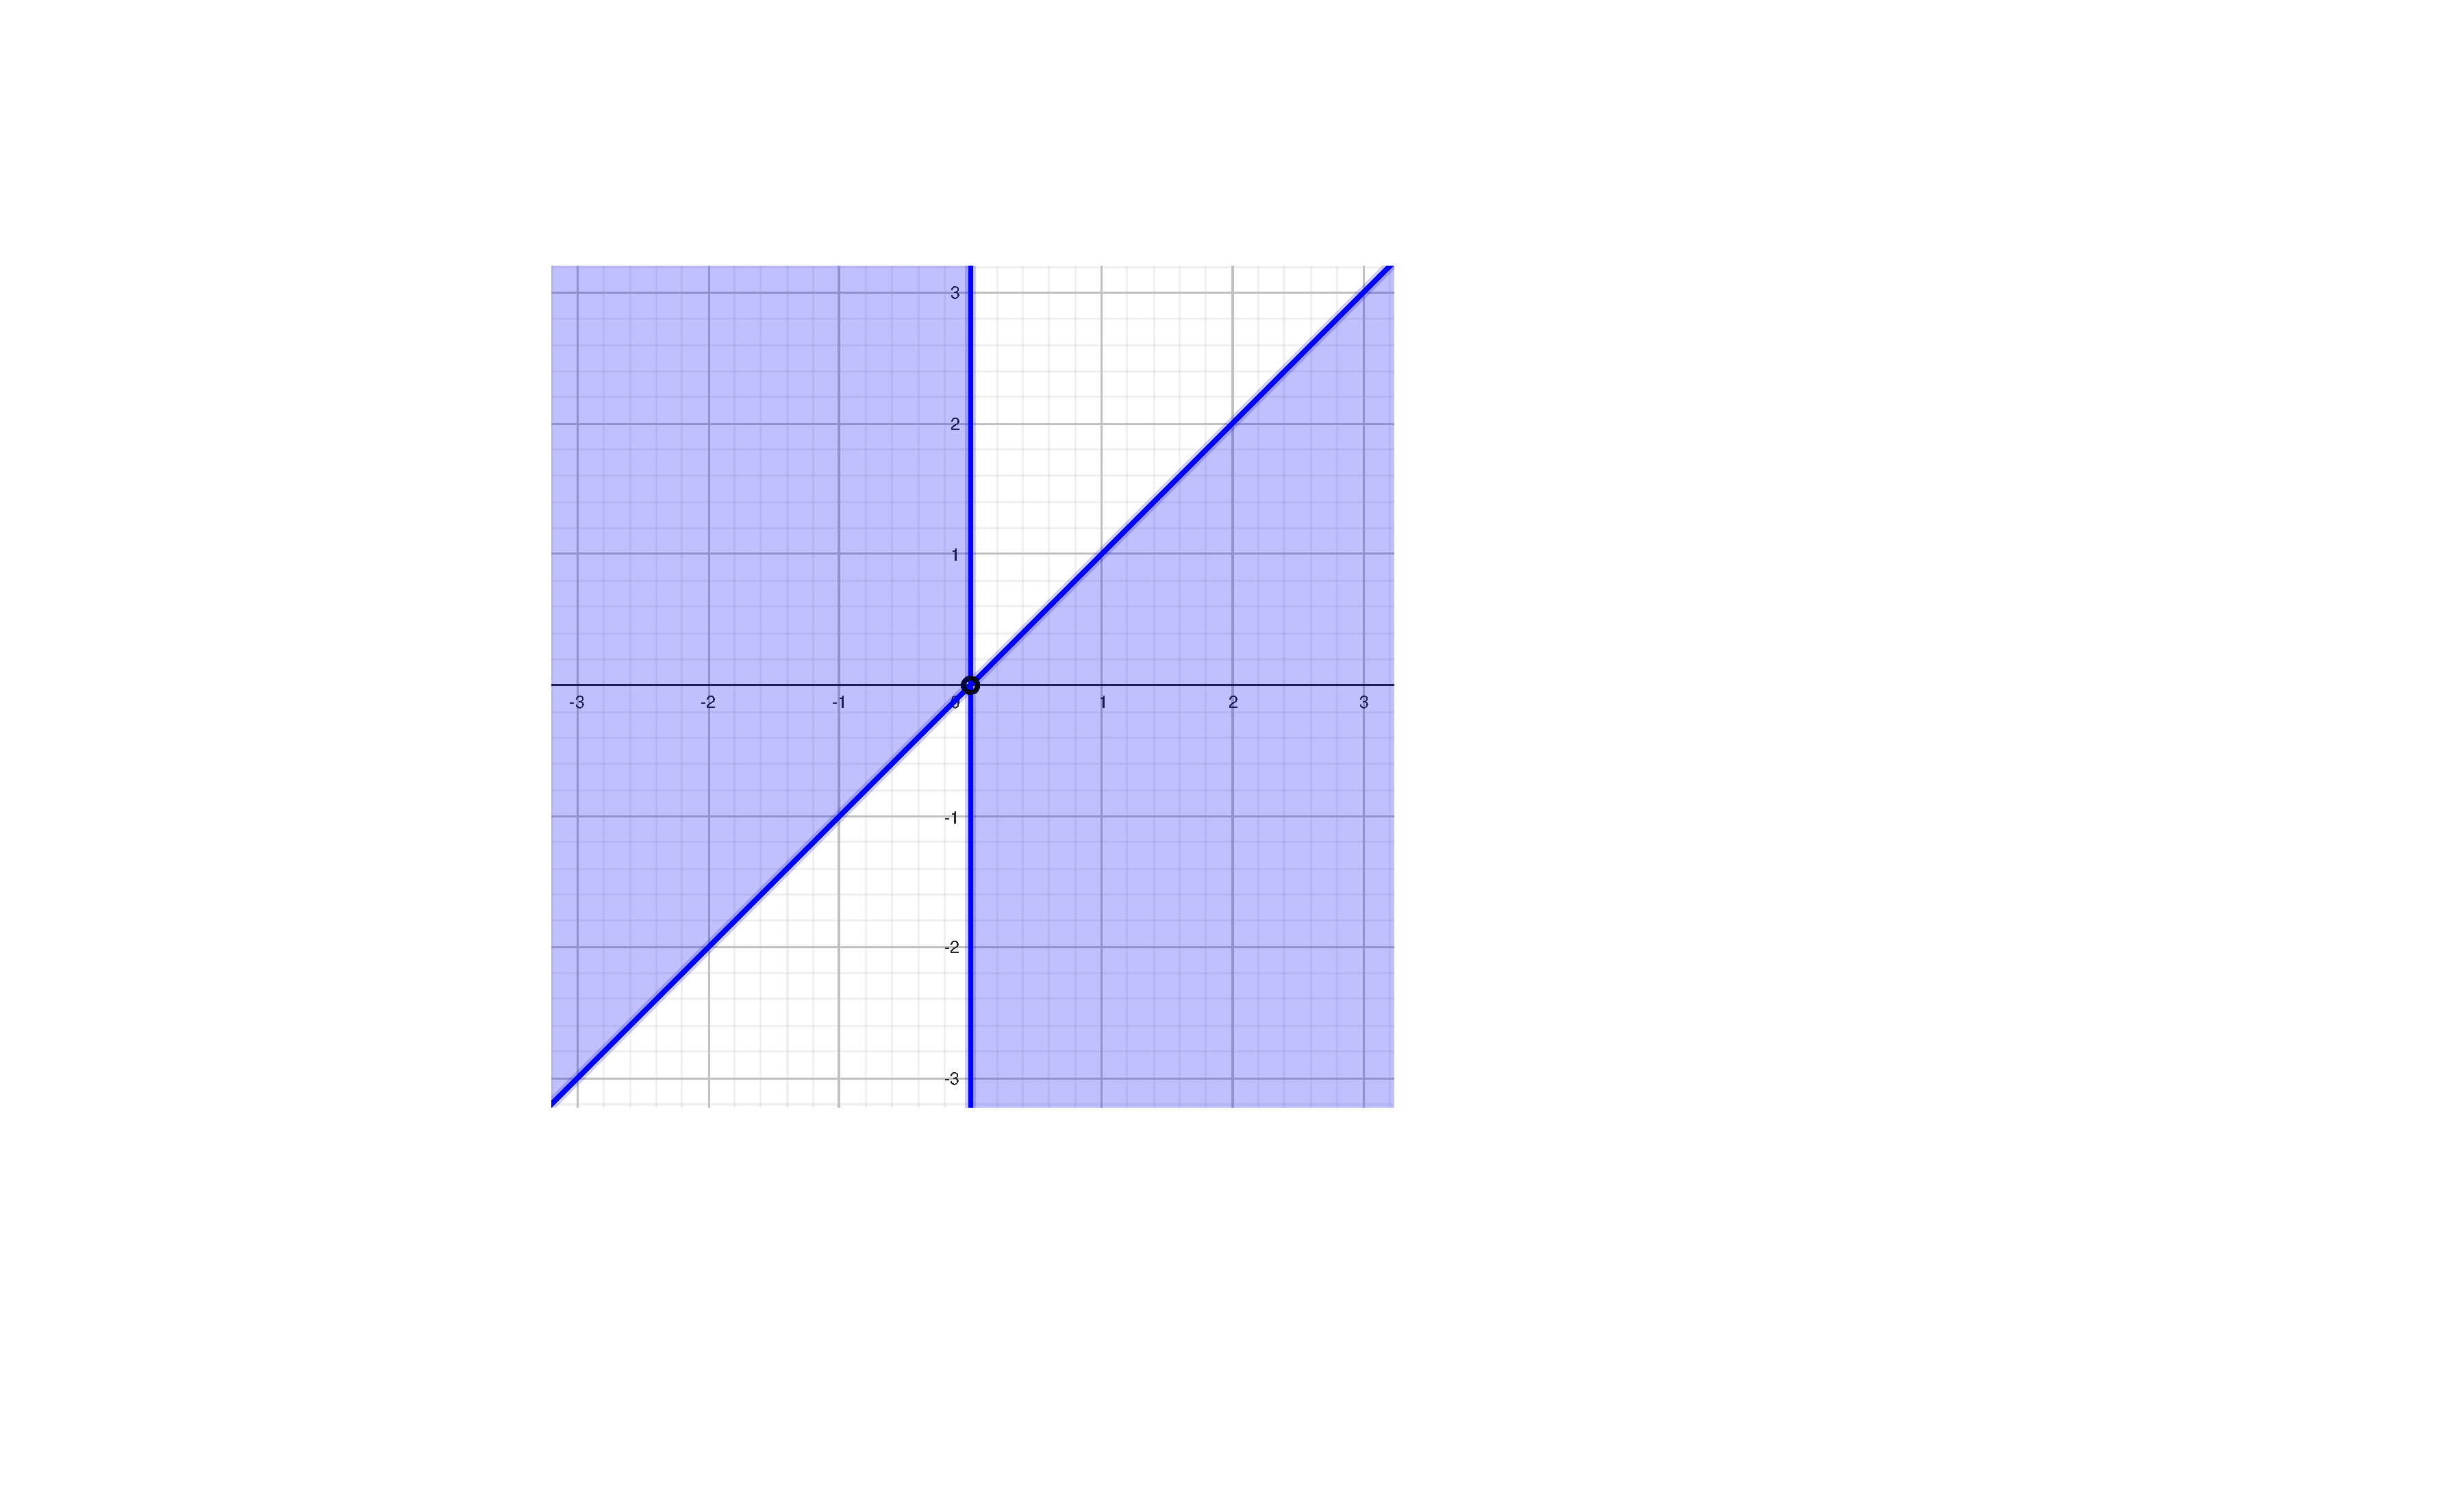
\includegraphics[width=.7\textwidth]{img/limiti-1.pdf}
	\end{figure}

	\noindent
	Per verificare l'esistenza del limite, si può verificare andando a sostituire parzialmente con $y = 0$:
	\begin{equation*}
		\displaystyle\lim_{x \rightarrow 0} f\left(x,0\right) = \dfrac{\sqrt{x\left(x-0\right)}}{x^{2}+0^{2}} = \dfrac{\sqrt{x^{2}}}{x^{2}} = \dfrac{x}{x^{2}} = \dfrac{1}{x} = \dfrac{1}{0^{+}} = +\infty
	\end{equation*}
	Ricordando che $0^{+}$ è un numero che corrisponde a $0,00\cdots001$. Per cui, un numero diviso $0^{+}$ risulta infinito. Per quanto riguarda $x = 0$:
	\begin{equation*}
		\displaystyle\lim_{y \rightarrow 0} f\left(0,y\right) = \dfrac{0}{0^{2} + y^{2}} = \dfrac{0}{y^{2}} = 0
	\end{equation*}
	Il risultato dei due limiti è differente, per cui il limite non esiste.\newpage

	\subsubsection{Manipolazioni algebriche}\label{subsubsection: manipolazioni algebriche}

	Per verificare l'esistenza di limiti per funzioni di due variabili, spesso si utilizzano tecniche di manipolazione algebrica per ottenere forme più convenienti.\newline

	\begin{flushleft}
		\example{\underline{Esempio 1}}
	\end{flushleft}
	Il seguente limite, se sostituito immediatamente si ottiene la forma indeterminata:
	\begin{equation*}
		\displaystyle\lim_{\left(x,y\right) \rightarrow \left(1,1\right)} \dfrac{x^{2}y^{3} - x^{3}y^{2}}{x^{2} - y^{2}} = \dfrac{1^2 \cdot 1^{3} - 1^{3} \cdot 1^{2}}{1^{2} - 1^{2}} = \dfrac{0}{0}
	\end{equation*}
	Con alcune manipolazioni algebriche si può ottenere la seguente forma:
	\begin{equation*}
		\dfrac{x^{2}y^{3} - x^{3}y^{2}}{x^{2} - y^{2}} = \dfrac{x^{2}y^{2}\left(y-x\right)}{\left(x+y\right)\left(x-y\right)} = \dfrac{\cancel{-} x^{2}y^{2}\cancel{\left(y-x\right)}}{- \left(x+y\right)\cancel{\left(x-y\right)}} = -\dfrac{x^{2}y^{2}}{x+y}
	\end{equation*}
	Andando a sostituire il limite si ottiene una forma determinata:
	\begin{equation*}
		\displaystyle\lim_{\left(x,y\right) \rightarrow \left(1,1\right)} -\dfrac{x^{2}y^{2}}{x+y} = - \dfrac{1}{2}
	\end{equation*}

	\begin{flushleft}
		\example{\underline{Esempio 2}}
	\end{flushleft}
	Il seguente limite ha forma indeterminata con una sostituzione immediata:
	\begin{equation*}
		\displaystyle\lim_{\left(x,y\right) \rightarrow \left(\pi, \frac{\pi}{2}\right)} \dfrac{\cos\left(y\right) - \sin\left(2y\right)}{\cos\left(x\right)\cos\left(y\right)} = \dfrac{\cos\left(\frac{\pi}{2}\right) - \sin\left(2 \cdot \frac{\pi}{2}\right)}{\cos\left(\pi\right)\cos\left(\frac{\pi}{2}\right)} = \dfrac{0 - 0}{-1\cdot 0} = \dfrac{0}{0}
	\end{equation*}
	Si eseguono alcune manipolazioni algebriche:
	\begin{equation*}
		\dfrac{\cos\left(y\right) - \sin\left(2y\right)}{\cos\left(x\right)\cos\left(y\right)} = 
		\dfrac{\cos\left(y\right) - 2 \sin\left(y\right) \cos\left(y\right)}{\cos\left(x\right)\cos\left(y\right)} =
		\dfrac{\cos\left(y\right)\left(1-2\sin\left(y\right)\right)}{\cos\left(x\right)\cos\left(y\right)} =
		\dfrac{1 - 2\sin\left(y\right)}{\cos\left(x\right)}
	\end{equation*}
	Andando a sostituire i valori del limite si ottiene una forma determinata:
	\begin{equation*}
		\displaystyle\lim_{\left(x,y\right) \rightarrow \left(\pi, \frac{\pi}{2}\right)} \dfrac{1 - 2\sin\left(y\right)}{\cos\left(x\right)} = +1
	\end{equation*}\newpage

	\subsubsection{Maggiorazioni utili per risolvere limiti e Teorema del confronto (dei due carabinieri)}\label{subsubsection: maggiorazioni utili per risolvere limiti e Teorema del confronto (dei due carabinieri)}

	Purtroppo, le manipolazioni algebriche talvolta non sono abbastanza. Risulta dunque necessario introdurre una nuova tecnica utilizzata in combo con un teorema famoso: il teorema del confronto o dei due carabinieri.
	\begin{theorem}[\textbf{Teorema del confronto}]
		Sia $x_{0} \in \mathbb{R}$ un punto di accumulazione per il dominio di tre funzioni: $f,g,h$. Le quali sono definite in un intorno di $x_{0}$ chiamato $I$. Ipotizzando che:
		\begin{enumerate}[label=\alph*)]
			\item Per ogni $x \in I$ la funzione $g\left(x\right)$ assuma valori non inferiori a $f\left(x\right)$ e non superiori a $h\left(x\right)$, ovverosia:
			\begin{equation*}
				f\left(x\right) \le g\left(x\right) \le h\left(x\right) \hspace{2em} \forall x \in I
			\end{equation*}

			\item I due limiti per $x$ tendente a $x_{0}$ di $f\left(x\right)$ e $h\left(x\right)$ esistano finiti e valgano entrambi $l$:
			\begin{equation*}
				\displaystyle\lim_{x\rightarrow x_{0}} f\left(x\right) = \displaystyle\lim_{x\rightarrow x_{0}} h\left(x\right) = l \hspace{2em} \text{con } l \in \mathbb{R}
			\end{equation*}
		\end{enumerate}
		Allora, sotto tali ipotesi, risulta che il limite per $x \rightarrow x_{0}$ di $g\left(x\right)$ vale $l$:
		\begin{equation*}
			\displaystyle\lim_{x\rightarrow x_{0}} g\left(x\right) = l
		\end{equation*}
	\end{theorem}
	Nel teorema vengono prese in considerazione tre funzioni definite in un intorno di $x_{0}$, la quale può essere un valore finito o infinito. La condizione importante per cui tale teorema sia veritiero, è che la seguente ipotesi sia vera:
	\begin{equation*}
		f\left(x\right) \le g\left(x\right) \le h\left(x\right)
	\end{equation*}
	Ovvero che $g$ \textbf{debba essere contenuta tra} $f$ \textbf{e} $h$. Per questo motivo, la funzione $f$ viene chiamata funzione \emph{\textbf{minorante}}, mentre la funzione $h$ viene chiamata funzione \emph{\textbf{maggiorante}} (questo è anche il motivo per cui si cercano \dquotes{maggiorazioni} per risolvere i limiti).\newline

	\noindent
	Il teorema si chiama \dquotes{dei due carabinieri} poiché è possibile immaginare le funzioni esterne ($f$ e $h$) come due carabinieri che accompagnano il detenuto ($g$) in prigione.\newline

	\noindent
	Alcune maggiorazioni utili da tenere a mente:
	\begin{itemize}
		\item $\left| x \pm y \right| \le \left| x \right| + \left| y \right|$ per ogni $\left(x,y\right) \in \mathbb{R}^{2}$
		
		\item $\left| xy \right| \le \dfrac{1}{2}\left(x^{2} + y^{2}\right)$ per ogni $\left(x,y\right) \in \mathbb{R}^{2}$

		\item $\left| x \right| \le \sqrt{x^{2} + y^{2}}$ per ogni $\left(x,y\right) \in \mathbb{R}^{2}$

		\item $-1 \le \sin\left(x\right) \le 1$ per ogni $x \in \mathbb{R}$

		\item $-1 \le \cos\left(x\right) \le 1$ per ogni $x \in \mathbb{R}$

		\item $\left| \sin\left(x\right) \right| \le \left| x \right|$ per ogni $x \in \mathbb{R}$
	\end{itemize}\newpage

	\begin{flushleft}
		\example{\underline{Esempio 1}}
	\end{flushleft}
	Calcolare, se esiste, il limite:
	\begin{equation*}
		\displaystyle\lim_{\left(x,y\right) \rightarrow \left(0,0\right)} f\left(x,y\right) \rightarrow f\left(x,y\right) = 
		\begin{cases}
			\dfrac{x^{4}+y^{4}}{x^{2}+y^{2}} 	& \left(x,y\right) \ne \left(0,0\right) \\ \\
			0									& \left(x,y\right) = \left(0,0\right)
		\end{cases}
	\end{equation*}
	Si può applicare il teorema del confronto. La funzione minorante può essere tranquillamente zero, mentre la funzione maggiorante è necessario calcolarla.
	\begin{equation*}
		0 \le \dfrac{x^{4}+y^{4}}{x^{2}+y^{2}} \le \: ???
	\end{equation*}
	La funzione maggiorante può essere la funzione originale ma con alcune manipolazioni algebriche:
	\begin{equation*}
		\dfrac{x^{4}+y^{4}}{x^{2}+y^{2}} = \dfrac{\left(x^{2}+y^{2}\right)^{2}}{x^{2}+y^{2}} = x^{2}+y^{2}
	\end{equation*}
	Per cui la base di partenza del teorema del confronto è:
	\begin{equation*}
		0 \le \dfrac{x^{4}+y^{4}}{x^{2}+y^{2}} \le x^{2}+y^{2}
	\end{equation*}
	Adesso si può verificare il limite per gli estremi e se i risultati rispettano la disuguaglianza, allora si può affermare che esiste. Il limite di $0$ è immediato, mentre il limite di $x^{2} + y^{2}$ è:
	\begin{equation*}
		\displaystyle\lim_{\left(x,y\right) \rightarrow \left(0,0\right)} x^{2} + y^{2} = 0^{2} + 0^{2} = 0
	\end{equation*}
	Per cui, grazie al teorema del confronto è possibile affermare che:
	\begin{equation*}
		\begin{array}{rcccl}
			0 &\le& \dfrac{x^{4}+y^{4}}{x^{2}+y^{2}} &\le& x^{2}+y^{2} \\ [1em]
			%
			\displaystyle\lim_{\left(x,y\right)\rightarrow\left(0,0\right)} 0 &\le& \displaystyle\lim_{\left(x,y\right)\rightarrow\left(0,0\right)}\dfrac{x^{4}+y^{4}}{x^{2}+y^{2}} &\le& \displaystyle\lim_{\left(x,y\right)\rightarrow\left(0,0\right)}x^{2}+y^{2} \\ [1em]
			%
			0 &\le& \dfrac{x^{4}+y^{4}}{x^{2}+y^{2}} &\le& 0
		\end{array}
	\end{equation*}
	Il limite esiste ed è uguale a zero:
	\begin{equation*}
		\displaystyle\lim_{\left(x,y\right) \rightarrow \left(0,0\right)} f\left(x,y\right) = 0
	\end{equation*}
	Inoltre la funzione è continua.\newpage

	\begin{flushleft}
		\example{\underline{Esempio 2}}
	\end{flushleft}
	Calcolare, se esiste, il limite:
	\begin{equation*}
		\displaystyle\lim_{\left(x,y\right) \rightarrow \left(0,0\right)} f\left(x,y\right) \rightarrow f\left(x,y\right) = 
		\begin{cases}
			\dfrac{x^{2}}{\sqrt{x^{2} + y^{2}}}	& \left(x,y\right) \ne \left(0,0\right) \\ \\
			0									& \left(x,y\right) = \left(0,0\right)
		\end{cases}
	\end{equation*}
	Si può applicare il teorema del confronto. La funzione minorante può essere tranquillamente zero, mentre la funzione maggiorante è necessario calcolarla.
	\begin{equation*}
		0 \le \dfrac{x^{2}}{\sqrt{x^{2} + y^{2}}} \le \: ???
	\end{equation*}
	La funzione maggiorante può essere ottenuta grazie alla maggiorazione $x^{2} + y^{2}$, ovvero aggiungendo una $y^{2}$:
	\begin{equation*}
		0 \le \dfrac{x^{2}}{\sqrt{x^{2} + y^{2}}} \le \dfrac{x^{2} + y^{2}}{\sqrt{x^{2} + y^{2}}}
	\end{equation*}
	Il denominatore e il numeratore si possono semplificare:
	\begin{equation*}
		0 \le \dfrac{x^{2}}{\sqrt{x^{2} + y^{2}}} \le \sqrt{x^{2}+y^{2}}
	\end{equation*}
	Adesso si può verificare il limite per gli estremi e se i risultati rispettano la disuguaglianza, allora si può affermare che esiste. Il limite di $0$ è immediato, mentre il limite di $\sqrt{x^{2} + y^{2}}$ è:
	\begin{equation*}
		\displaystyle\lim_{\left(x,y\right) \rightarrow \left(0,0\right)} \sqrt{x^{2} + y^{2}} = \sqrt{0^{2} + 0^{2}} = 0
	\end{equation*}
	Per cui, grazie al teorema del confronto è possibile affermare che:
	\begin{equation*}
		\begin{array}{rcccl}
			0 &\le& \dfrac{x^{2}}{\sqrt{x^{2} + y^{2}}} &\le& \sqrt{x^{2}+y^{2}} \\ [1em]
			%
			\displaystyle\lim_{\left(x,y\right)\rightarrow\left(0,0\right)} 0 &\le& \displaystyle\lim_{\left(x,y\right)\rightarrow\left(0,0\right)}\dfrac{x^{2}}{\sqrt{x^{2} + y^{2}}} &\le& \displaystyle\lim_{\left(x,y\right)\rightarrow\left(0,0\right)} \sqrt{x^{2}+y^{2}} \\ [1em]
			%
			0 &\le& \dfrac{x^{2}}{\sqrt{x^{2} + y^{2}}} &\le& 0
		\end{array}
	\end{equation*}
	Il limite esiste ed è uguale a zero:
	\begin{equation*}
		\displaystyle\lim_{\left(x,y\right) \rightarrow \left(0,0\right)} f\left(x,y\right) = 0
	\end{equation*}
	E la funzione è continua. In questo esempio, la maggiorazione è stata applicata con l'intuito, ovvero con l'intento di riuscire a semplificare il denominatore così da non avere forme indeterminate nel caso di sostituzione.\newpage

	\begin{flushleft}\label{limiti: esempio 3}
		\example{\underline{Esempio 3}}
	\end{flushleft}
	Calcolare, se esiste, il limite:
	\begin{equation*}
		\displaystyle\lim_{\left(x,y\right) \rightarrow \left(0,0\right)} f\left(x,y\right) \rightarrow f\left(x,y\right) = 
		\begin{cases}
			\dfrac{x^{4}y^{4}}{x^{2} + y^{4}}	& \left(x,y\right) \ne \left(0,0\right) \\ \\
			0										& \left(x,y\right) = \left(0,0\right)
		\end{cases}
	\end{equation*}
	Si può applicare il teorema del confronto. La funzione minorante può essere tranquillamente zero, mentre la funzione maggiorante è necessario calcolarla.
	\begin{equation*}
		0 \le \dfrac{x^{4}y^{4}}{x^{2} + y^{4}} \le \: ???
	\end{equation*}
	La funzione maggiorante può essere ottenuta con un piccolo ragionamento. Osservando bene, si può scompattare la frazione e notare che un valore ($y$) diviso lo stesso valore ma aumentato di un'unità sempre positiva ($x^{2}+y$), è sempre minore uguale a $1$. Questo perché il numeratore sarà sempre minore o uguale al denominatore:
	\begin{equation*}
		\dfrac{y^{4}}{x^{2}+y^{4}} \le 1
	\end{equation*}
	Quindi, un'unità che è $1$ o minore, sarà sempre minore o uguale ad un valore elevato alla $4$. Formalmente:
	\begin{equation*}
			0 \le \dfrac{x^{4}y^{4}}{x^{2}+y^{4}} = \underbrace{\dfrac{y^{4}}{x^{2}+y^{4}}}_{\le 1} \cdot x^{4} \le x^{4}
	\end{equation*}
	Adesso si può verificare il limite per gli estremi e se i risultati rispettano la disuguaglianza, allora si può affermare che esiste. Il limite di $0$ è immediato, mentre il limite di $x^{4}$ è zero. Ne consegue che:
	\begin{equation*}
		\begin{array}{rcccl}
			0 &\le& \dfrac{y^{4}}{x^{2}+y^{4}} \cdot x^{4} &\le& x^{4} \\ [1em]
			%
			\displaystyle\lim_{\left(x,y\right)\rightarrow\left(0,0\right)} 0 &\le& \displaystyle\lim_{\left(x,y\right)\rightarrow\left(0,0\right)}\dfrac{y^{4}}{x^{2}+y^{4}} \cdot x^{4} &\le& \displaystyle\lim_{\left(x,y\right)\rightarrow\left(0,0\right)} x^{4} \\ [1em]
			%
			0 &\le& \dfrac{y^{4}}{x^{2}+y^{4}} \cdot x^{4} &\le& 0
		\end{array}
	\end{equation*}
	Il limite esiste ed è uguale a zero:
	\begin{equation*}
		\displaystyle\lim_{\left(x,y\right) \rightarrow \left(0,0\right)} f\left(x,y\right) = 0
	\end{equation*}
	E la funzione è continua. Anche in questo esempio, la maggiorazione è stata applicata con l'intuito, ovvero con l'intento di riuscire a imporre una maggiorazione.\newpage

	\begin{flushleft}
		\example{\underline{Esempio 4}}
	\end{flushleft}
	Calcolare, se esiste, il limite:
	\begin{equation*}
		\displaystyle\lim_{\left(x,y\right) \rightarrow \left(0,0\right)} f\left(x,y\right) \rightarrow f\left(x,y\right) = 
		\begin{cases}
			\dfrac{\sin\left(xy\right)}{\sqrt{\left| x y \right|}}	& \left(x,y\right) \ne \left(0,0\right) \\ \\
			0										& \left(x,y\right) = \left(0,0\right)
		\end{cases}
	\end{equation*}
	Si può applicare il teorema del confronto. La funzione minorante può essere tranquillamente zero, mentre la funzione maggiorante è necessario calcolarla.
	\begin{equation*}
		0 \le \dfrac{x^{4}y^{4}}{x^{2} + y^{4}} \le \: ???
	\end{equation*}
	La funzione maggiorante può essere ottenuta guardando le maggiorazioni ad inizio capitolo. Infatti, il seno è possibile riscriverlo come il valore assoluto del suo argomento:
	\begin{equation*}
		\left|\dfrac{\sin\left(xy\right)}{\sqrt{\left| x y \right|}}\right| \le \dfrac{\left|xy\right|}{\sqrt{\left| x y \right|}}
	\end{equation*}
	Semplificando il numeratore con il denominatore (perché un valore diviso per la sua radice quadrata restituisce il risultato della radice quadrata):
	\begin{equation*}
		\sqrt{\left| xy \right|}
	\end{equation*}
	Adesso si può verificare il limite per gli estremi e se i risultati rispettano la disuguaglianza, allora si può affermare che esiste. Il limite di $0$ è immediato, mentre il limite di $\sqrt{\left| xy \right|}$ è zero. Ne consegue che:
	\begin{equation*}
		\begin{array}{rcccl}
			0 &\le& \dfrac{\sin\left(xy\right)}{\sqrt{\left| x y \right|}} &\le& \sqrt{\left| xy \right|} \\ [1.5em]
			%
			\displaystyle\lim_{\left(x,y\right)\rightarrow\left(0,0\right)} 0 
			&\le& 
			\displaystyle\lim_{\left(x,y\right)\rightarrow\left(0,0\right)} \dfrac{\sin\left(xy\right)}{\sqrt{\left| x y \right|}} 
			&\le& 
			\displaystyle\lim_{\left(x,y\right)\rightarrow\left(0,0\right)} \sqrt{\left| xy \right|} \\ [1.5em]
			%
			0 &\le& \dfrac{\sin\left(xy\right)}{\sqrt{\left| x y \right|}} &\le& 0
		\end{array}
	\end{equation*}
	Il limite esiste ed è uguale a zero:
	\begin{equation*}
		\displaystyle\lim_{\left(x,y\right) \rightarrow \left(0,0\right)} f\left(x,y\right) = 0
	\end{equation*}
	E la funzione è continua. A differenza degli altri esempi, qui la maggiorazione è stata applicata ricordandosi una maggiorazione nota.\newpage

	\begin{flushleft}
		\example{\underline{Esempio 5}}
	\end{flushleft}
	Calcolare, se esiste, il limite:
	\begin{equation*}
		\displaystyle\lim_{\left(x,y\right) \rightarrow \left(0,0\right)} f\left(x,y\right) \rightarrow f\left(x,y\right) = \dfrac{
				x^{6} + 3y^{3} - 3x^{2} - 3y^{2}
			}{x^{2}+y^{2}}
	\end{equation*}
	Si può applicare il teorema del confronto. Ma prima di partire è necessario capire dove applicarlo. La funzione maggiorante può essere ottenuta notando che la frazione può essere riscritta in un altro modo:
	\begin{equation*}
		\dfrac{
				x^{6} + 3y^{3} - 3x^{2} - 3y^{2}
		}{x^{2}+y^{2}}
		=
		\dfrac{
			x^{6} + 3y^{3} -3 \left(x^{2} + y^{2}\right)
		}{x^{2}+y^{2}} =
		\dfrac{x^{6} + 3y^{3}}{x^{2}+y^{2}} - \underbrace{\dfrac{3 \left(x^{2} + y^{2}\right)}{x^{2}+y^{2}}}_{3}
	\end{equation*}
	Il valore $-3$ è una costante e non dipende da nessuna variabile! Per cui adesso si sposta l'attenzione sulla frazione. Essa può essere riscritta come:
	\begin{equation*}
		\dfrac{x^{6} + 3y^{3}}{x^{2}+y^{2}} = \dfrac{x^{6}}{x^{2}+y^{2}} + \dfrac{3y^{3}}{x^{2}+y^{2}} = x^{4} \cdot \dfrac{x^{2}}{x^{2}+y^{2}} + \dfrac{y^{2}}{x^{2}+y^{2}} \cdot 3|y|
	\end{equation*}
	Come accadeva nell'esempio 3 a pagina \pageref{limiti: esempio 3}, le due frazioni hanno un valore minore o uguale a $1$ poiché il numeratore sarà sempre minore del denominatore. Quindi, si può considerare solo i valori moltiplicati, e applicare il teorema del confronto:
	\begin{equation*}
		\begin{array}{rcccl}
			0 
			&\le& 
			\dfrac{x^{6} + 3y^{3}}{x^{2}+y^{2}}
			&\le& x^{4} + 3|y| \\ [1.5em]
			%
			\displaystyle\lim_{\left(x,y\right)\rightarrow\left(0,0\right)} 0 
			&\le& 
			\displaystyle\lim_{\left(x,y\right)\rightarrow\left(0,0\right)} \dfrac{x^{6} + 3y^{3}}{x^{2}+y^{2}}
			&\le& 
			\displaystyle\lim_{\left(x,y\right)\rightarrow\left(0,0\right)} x^{4} + 3|y| \\ [1.5em]
			%
			0 &\le& \dfrac{x^{6} + 3y^{3}}{x^{2}+y^{2}} &\le& 0
		\end{array}
	\end{equation*}
	Il limite di quella frazione è uguale a zero. Ma attenzione, il risultato finale è diverso. Si ricorda che era stato rimosso il valore $-3$ poiché era una costante. Quindi il risultato del limite della funzione è $-3$:
	\begin{gather*}
		\dfrac{
				x^{6} + 3y^{3} - 3x^{2} - 3y^{2}
		}{x^{2}+y^{2}} = \dfrac{x^{6} + 3y^{3}}{x^{2}+y^{2}} - 3 \\ \\
		\displaystyle\lim_{\left(x,y\right) \rightarrow \left(0,0\right)} f\left(x,y\right) = \displaystyle\lim_{\left(x,y\right) \rightarrow \left(0,0\right)}\dfrac{x^{6} + 3y^{3}}{x^{2}+y^{2}} - 3 = -3
	\end{gather*}
	E la funzione è continua. Come negli altri esempi, qui la maggiorazione è stata applicata facendo alcune considerazioni su una parte di funzione.\newpage

	\subsubsection{Calcolo limiti in coordinate polari}\label{subsubsection: calcolo limiti in coordinate polari}

	Per studiare il comportamento di una funzione $f$ che da $\left(x,y\right) \rightarrow \left(a,b\right)$, si può vedere che cosa accade alla funzione:
	\begin{equation}
		F\left(\rho, \theta\right) = f\left(a + \rho\cos\left(\theta\right), b + \sin\left(\theta\right)\right)
	\end{equation}
	Quando $\rho$ tende a $0^{+}$.
	\begin{theorem}
		Se in un intorno di $\left(a,b\right)$ si ha $\left| F\left(\rho, \theta\right) - L \right| \le g\left(\rho\right)$ con $g\left(\rho\right) \rightarrow 0$ per $\rho$ che tende a $0^{+}$, allora:
		\begin{equation}
			\displaystyle\lim_{\left(x,y\right) \rightarrow \left(a,b\right)} f\left(x,y\right) = L
		\end{equation}
	\end{theorem}

	\noindent
	Da notare che quello che il teorema esprime è:
	\begin{equation*}
		\displaystyle\lim_{\rho \rightarrow 0^{+}} F\left(\rho,\theta\right) = L
	\end{equation*}
	\textbf{Uniformemente} rispetto a $\theta$.\newline
	
	\noindent
	In parole povere il teorema può essere riscritto come: se in un intorno di $\left(a,b\right)$ si ha
	\begin{equation*}
		\left| F\left(r, \theta\right) - L \right| \le g\left(r\right) \hspace{2em} \text{con} \hspace{2em} \displaystyle\lim_{r \rightarrow 0^{+}} g\left(r\right) = 0
	\end{equation*}
	Allora:
	\begin{equation*}
		\displaystyle\lim_{\left(x,y\right) \rightarrow \left(a,b\right)} f\left(x,y\right) = L
	\end{equation*}
	\framedtext{%
		\underline{\textbf{N.B.}}: si ricorda che per passare alle coordinate polari bisogna trasformare la $x$ e la $y$ in:
		\begin{equation*}
			\begin{cases}
				x = a + \rho\cos\left(\theta\right) \\
				y = b + \rho\sin\left(\theta\right)
			\end{cases}
		\end{equation*}
		Dove $a$ e $b$ sono le coordinate in cui viene definito il limite
	}\:\newline

	\noindent
	Nelle seguenti pagine si riportano alcuni esempi di limiti risolti con le coordinate polari (il limite numero 4 è importante come esempio):
	\begin{enumerate}
		\item $\displaystyle\lim_{\left(x,y\right) \rightarrow \left(0,0\right)} \dfrac{xy}{\sqrt{x^{2} + y^{2}}} = 0$
		\item $\displaystyle\lim_{\left(x,y\right) \rightarrow \left(0,1\right)} \dfrac{x^{2}}{\sqrt{x^{2} + \left(y-1\right)^{2}}} = 0$
		\item $\displaystyle\lim_{\left(x,y\right) \rightarrow \left(2,-1\right)} \dfrac{\left(x-2\right)^{3} + 4\left(x-2\right)^{2} + 4\left(y+1\right)^{2}}{\left(x-2\right)^{2} + \left(y+1\right)^{2}} = 4$
		\item $\displaystyle\lim_{\left(x,y\right) \rightarrow \left(0,0\right)} \dfrac{xy^{2}}{x^{2} + y^{4}} = 0$
	\end{enumerate}\newpage

	\begin{flushleft}
		\example{\underline{Esempio 1}}
	\end{flushleft}
	Verificare il risultato del limite:
	\begin{equation*}
		\displaystyle\lim_{\left(x,y\right) \rightarrow \left(0,0\right)} \dfrac{xy}{\sqrt{x^{2} + y^{2}}} = 0
	\end{equation*}
	Si applica il teorema per i limiti in coordinate polari. Per cui, la funzione, ovvero la frazione, meno il suo risultato, in questo caso $0$, deve essere minore o uguale alla funzione $g\left(r\right)$, in questo caso l'incognita da trovare. Ovviamente la funzione $g$ deve avere il limite per $0^{+}$ che è uguale a zero. Prima di tutto si riscrive l'espressione con le coordinate polari:
	\begin{equation*}
		\dfrac{xy}{\sqrt{x^{2} + y^{2}}} \rightarrow F\left(r, \theta\right) = \dfrac{r\cos\left(\theta\right) \cdot r\sin\left(\theta\right)}{\sqrt{\left(r \cos\left(\theta\right)\right)^{2} + \left(r \sin\left(\theta\right)\right)^{2}}}
	\end{equation*}
	Poi si eseguono alcune manipolazioni algebriche:
	\begin{gather*}
		\dfrac{r^{2} \cos\left(\theta\right)\sin\left(\theta\right)}{\sqrt{r^{2}\cos^{2}\left(\theta\right) + r^{2}\sin^{2}\left(\theta\right)}}
		=
		\dfrac{r^{2} \cos\left(\theta\right)\sin\left(\theta\right)}{\sqrt{r^{2} \left(\cos^{2}\left(\theta\right)+ \sin^{2}\left(\theta\right)\right)}}
		=
		\dfrac{r^{2} \cos\left(\theta\right)\sin\left(\theta\right)}{\sqrt{r^{2} \cdot 1}} \\ \\
		%
		\dfrac{r^{2}}{\sqrt{r^{2}}} \cdot \cos\left(\theta\right)\sin\left(\theta\right) = \sqrt{r^{2}} \cdot \cos\left(\theta\right)\sin\left(\theta\right)
	\end{gather*}
	Per definizione del seno e del coseno, si è certi che la funzione $F\left(r,\theta\right)$ è sicuramente minore o uguale a $\sqrt{r^{2}}$:
	\begin{equation*}
		0 \le \left| F\left(r,\theta\right) - L \right| \le \sqrt{r^{2}}
	\end{equation*}
	Il risultato del limite che tende a $0^{+}$ su $\sqrt{r^{2}}$ è zero. Inoltre, dipende solo da $r$ e non da $\theta$, per cui è una condizione abbastanza forte per dire che il limite esiste ed è uguale a zero (in riferimento a $f\left(x,y\right)$).\newpage

	\begin{flushleft}
		\example{\underline{Esempio 2}}
	\end{flushleft}
	Verificare che il limite esista e valga zero:
	\begin{equation*}
		\displaystyle\lim_{\left(x,y\right) \rightarrow \left(0,1\right)} \dfrac{x^{2}}{\sqrt{x^{2} + \left(y-1\right)^{2}}}
	\end{equation*}
	In questo caso le coordinate polari saranno $r \cos\left(\theta\right)$ e $1 + r\sin\left(\theta\right)$. Questo perché il limite tende a $a=0$ e $b=1$:
	\begin{equation*}
		0 \le \left| \dfrac{r^{2} \cos^{2}\left(\theta\right)}{\sqrt{r^{2} \cos^{2}\left(\theta\right) + \left(1 + r \sin\left(\theta\right)-1\right)^{2}}} \right| \le \: ???
	\end{equation*}
	Si semplifica la frazione:
	\begin{equation*}
		\left| \dfrac{r^{2} \cos^{2}\left(\theta\right)}{\sqrt{r^{2} \cos^{2}\left(\theta\right) + r^{2} \sin^{2}\left(\theta\right)}} \right| = \left| \dfrac{r^{2} \cos^{2}\left(\theta\right)}{\sqrt{r^{2}}} \right| = \left| \dfrac{r^{2} \cos^{2}\left(\theta\right)}{r} \right| = r \cos^{2}\left(\theta\right)
	\end{equation*}
	Il valore trovato è sicuramente sempre minore o uguale a $r$:
	\begin{equation*}
		0 \le r \cos^{2}\left(\theta\right) \le r
	\end{equation*}
	Il limite in $r$ di $0^{+}$ è sempre $0^{+}$. Per cui, il limite della funzione esiste ed è uguale a zero.\newpage

	\begin{flushleft}
		\example{\underline{Esempio 3}}
	\end{flushleft}
	Verificare che il limite esista e valga $4$:
	\begin{equation*}
		\displaystyle\lim_{\left(x,y\right) \rightarrow \left(2,-1\right)} \dfrac{\left(x-2\right)^{3} + 4\left(x-2\right)^{2} + 4\left(y+1\right)^{2}}{\left(x-2\right)^{2} + \left(y+1\right)^{2}}
	\end{equation*}
	Si riscrive la funzione con le coordinate polari:
	\begin{gather*}
		\begin{cases}
			x = 2 + r\cos\left(\theta\right) \\
			y = -1 + r\sin\left(\theta\right)
		\end{cases} \\
		\begin{array}{rcl}
			\dfrac{r^{3}\cos^{3}\left(\theta\right) + 4 r^{2} \cos^{2}\left(\theta\right) + 4 r^{2} \sin^{2}\left(\theta\right)}{r^{2} \cos^{2}\left(\theta\right) + r^{2} \sin^{2}\left(\theta\right)} 
			&=&
			\dfrac{
				r^{3}\cos^{3}\left(\theta\right) + 4r^{2}\left(\cos^{2}\left(\theta\right) + \sin^{2}\left(\theta\right)\right)
			}{
				r^{2}\left(\cos^{2}\left(\theta\right) + \sin^{2}\left(\theta\right)\right)
			} \\ [1.5em]
			%
			&=&
			\dfrac{r^{3}\cos^{3}\left(\theta\right) + 4r^{2}}{r^{2}} \\ [1.5em]
			%
			&=& \dfrac{r^{3}\cos^{3}\left(\theta\right)}{r^{2}} + \dfrac{4r^{2}}{r^{2}} \\ [1.5em]
			%
			&=& r \cos^{3}\left(\theta\right) + 4
		\end{array}
	\end{gather*}
	A questo punto, si può notare che la formula $\left| F\left(r,\theta\right) - L \right|$ prevede $- L$, che in questo esempio è identificato dal $+4$ ottenuto nell'ultimo passaggio. Per cui:
	\begin{equation*}
		\left| F\left(r,\theta\right) - 4 \right| = \left| r \cos^{3}\left(\theta\right) \right|
	\end{equation*}
	Quel valore è sicuramente minore o uguale a $r$ (classico ragionamento fatto anche per gli esercizi precedenti):
	\begin{equation*}
		\left| r \cos^{3}\left(\theta\right) \right| \le r
	\end{equation*}
	E il limite di $r$ in $0^{+}$ è uguale a $0^{+}$, ovvero un'unità infinitesima. L'esercizio si conclude affermando che il limite esiste e ha risultato uguale a $4$. Questo perché si considera $F-L$ e non solo la funzione $F$.

	\longline

	\begin{flushleft}
		\example{\underline{Esempio 4 (importante)}}
	\end{flushleft}
	Questo limite, a differenza degli altri, può essere risolto in maniera differente:
	\begin{equation*}
		\displaystyle\lim_{\left(x,y\right) \rightarrow \left(0,0\right)} \dfrac{xy^{2}}{x^{2} + y^{4}}
	\end{equation*}
	Nel caso in cui il limite esistesse, varrebbe zero. Questo perché la restrizione della funzione $f$ a qualunque retta passante per l'origine, porta a:
	\begin{equation*}
		\displaystyle\lim_{x \rightarrow 0} f\left(x,mx\right) = \displaystyle\lim_{x \rightarrow 0} \dfrac{mx^{3}}{x^{2} + m^{4}x^{4}} = \displaystyle\lim_{x \rightarrow 0} \dfrac{mx}{1 + m^{4}x^{2}} = 0
	\end{equation*}
	Qualunque sia $m \in \mathbb{R}$. Tuttavia, questo modo differente di dimostrare l'esistenza di un limite, non è una condizione sufficiente per concludere la dimostrazione. Infatti, nel caso in cui ci si muovesse lungo l'asse $y$ con $y = \sqrt{x}$ accadrebbe:
	\begin{equation*}
		\displaystyle\lim_{x \rightarrow 0^{+}} f\left(x, \sqrt{x}\right) = \displaystyle\lim_{x \rightarrow 0^{+}} \dfrac{x \cdot x}{x^{2} + x^{2}} = \displaystyle\lim_{x \rightarrow 0^{+}} \dfrac{x^{2}}{2x^{2}} = \dfrac{1}{2}
	\end{equation*}
	E questo dimostra che il limite originale non esiste.\newpage

	\subsection{Curve in $\mathbb{R}^{n}$}

	\begin{boxdef}
		Sia $I$ un intervallo della retta reale. Si chiama \definition{curva in $\mathbb{R}^{n}$} una funzione del tipo:
		\begin{equation}\label{eq: curva in Rn}
			\begin{array}{rcl}
				\gamma \: : \: I &\rightarrow& \mathbb{R}^{n} \\ [.5em]
				%
				t &\mapsto& \left(\gamma_{1}\left(t\right), \gamma_{2}\left(t\right), \cdots, \gamma_{n}\left(t\right)\right)
			\end{array}
		\end{equation}
		Che ha tutte le componenti $\gamma_{i} \: : \: I \rightarrow \mathbb{R}$ continue su $I$. Inoltre, viene detto \textbf{sostegno della curva} l'immagine di $\gamma$:
		\begin{equation}\label{eq: sostegno della curva}
			\gamma\left(I\right) = \left\{\gamma\left(t\right) \: : \: t \in I\right\}
		\end{equation}
	\end{boxdef}

	\noindent
	Con il termine \dquotes{curva} si intende una funzione di variabile reale\footnote{A ogni valore del parametro $t \in I$ è associato uno e un solo punto del sostegno.}, con \dquotes{sostegno di una curva} si intende un \textbf{insieme di punti} nello spazio euclideo.\newline

	\noindent
	Nel caso in cui l'insieme $I$ è chiuso e limitato, cioè $I = \left[a,b\right]$, si dice che la curva $\gamma$ è un \textbf{arco} o un \textbf{cammino continuo}. Inoltre, $\gamma\left(a\right)$ e $\gamma\left(b\right)$ sono estremi dell'arco (punto iniziale e punto finale). Alcuni esempi di parametrizzazione:
	\begin{figure}[!htp]
		\centering
		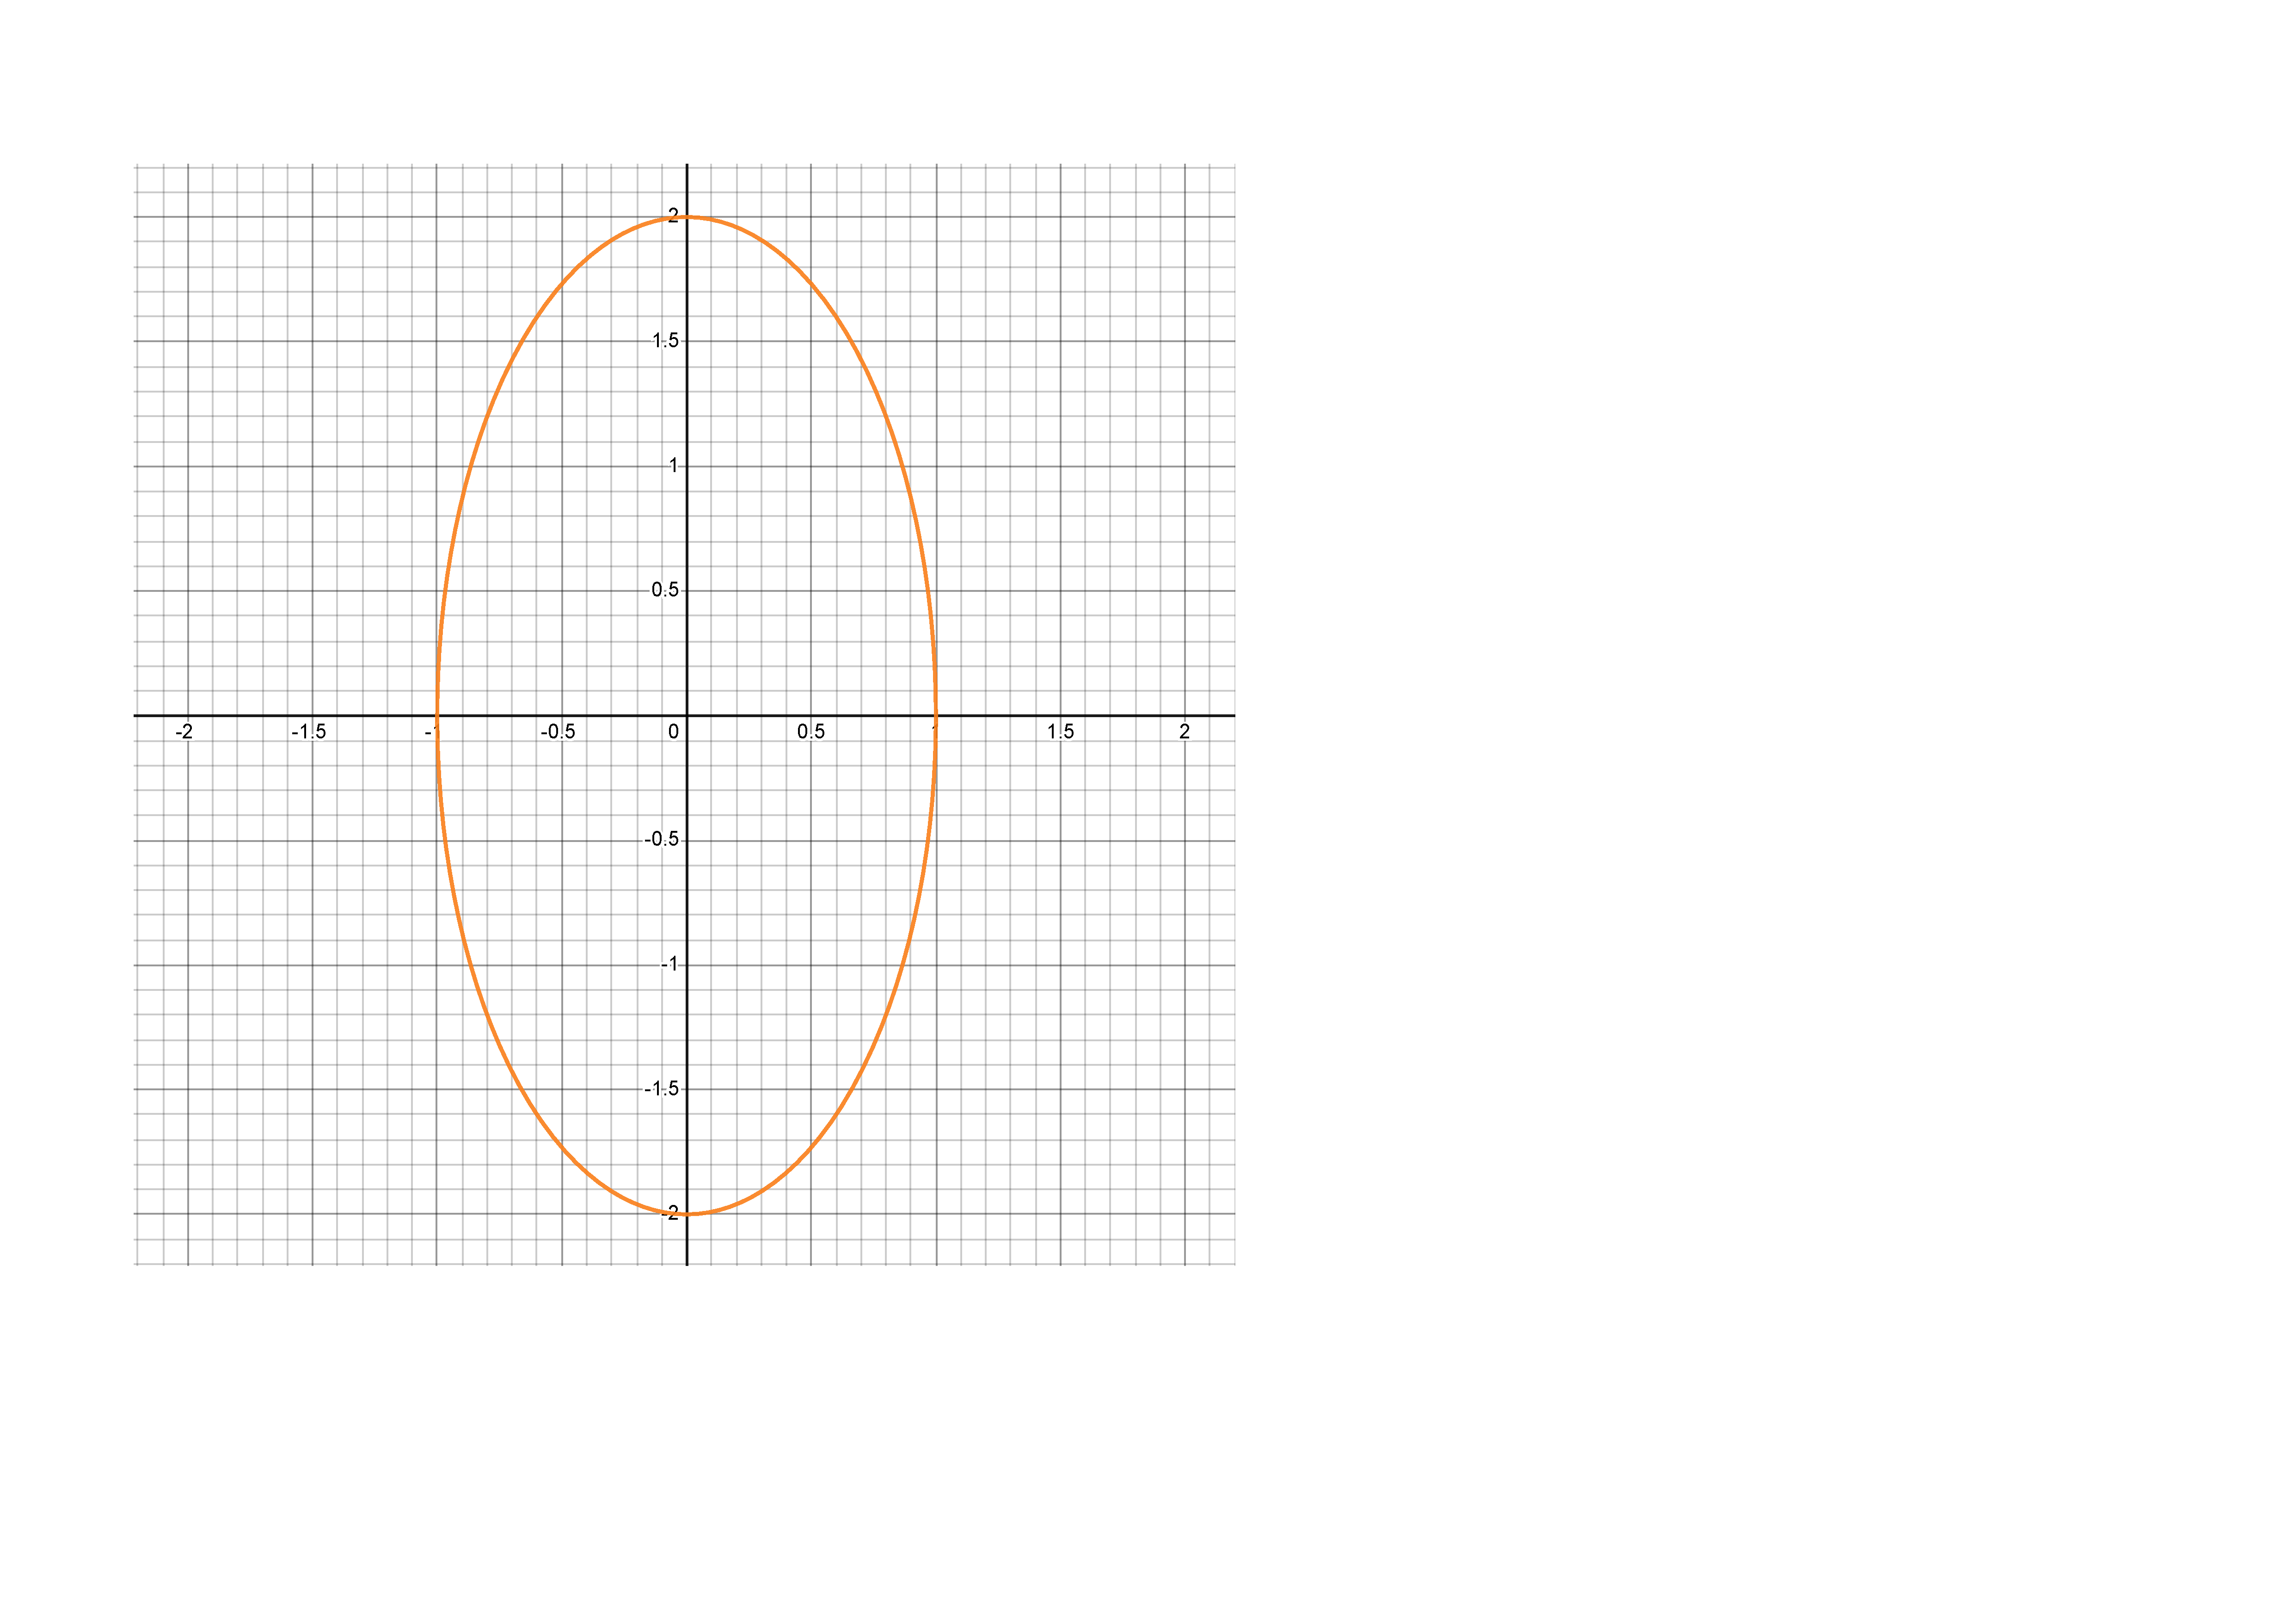
\includegraphics[width=.8\textwidth]{img/parametrizzazioni-1.pdf}
		\caption*{$\gamma: \left[0, 2\pi\right] \rightarrow \mathbb{R}^{2} \hspace{2em} t\mapsto\left(\cos\left(t\right), 2\sin\left(t\right)\right)$ è un cammino chiuso semplice.}
	\end{figure}\newpage

	\begin{figure}[!htp]
		\centering
		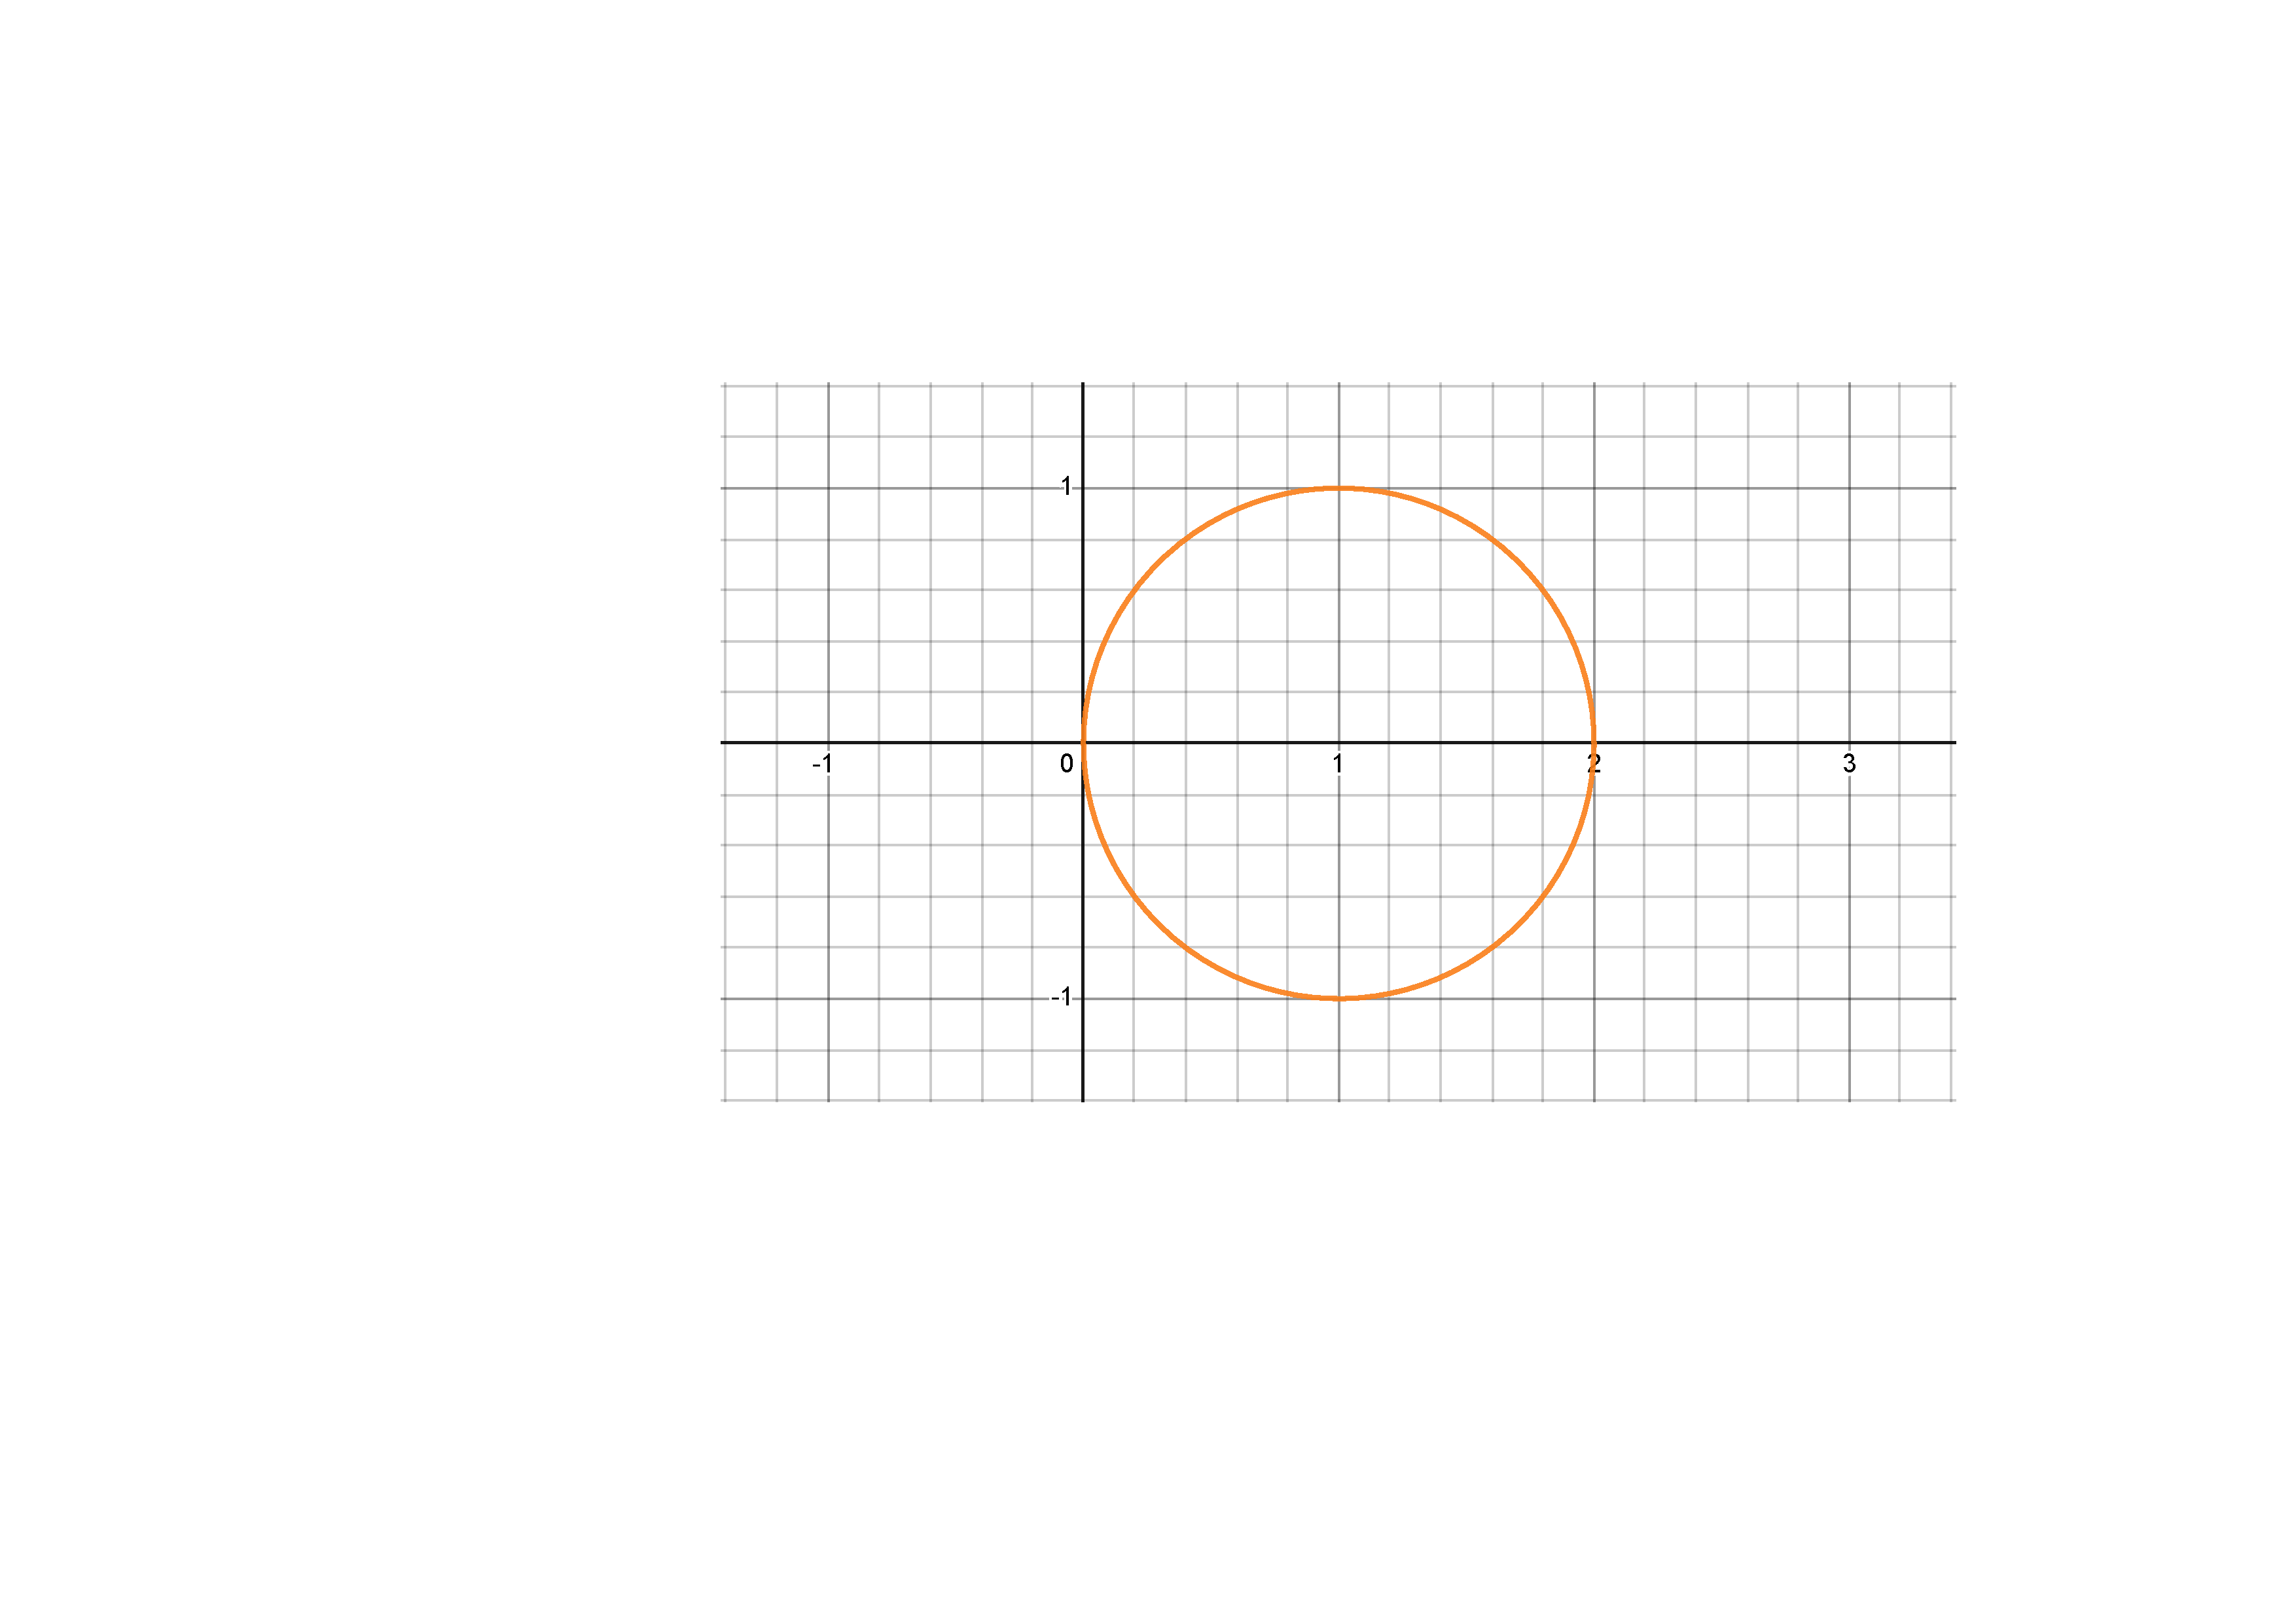
\includegraphics[width=.8\textwidth]{img/parametrizzazioni-2.pdf}
		\caption*{$\gamma: \left[0, \dfrac{\pi}{2}\right] \rightarrow \mathbb{R}^{2} \hspace{2em} t\mapsto\left(1+\cos\left(t\right), \sin\left(t\right)\right)$ è un arco di circonferenza semplice, ma non è chiuso.}
	\end{figure}

	\begin{figure}[!htp]
		\centering
		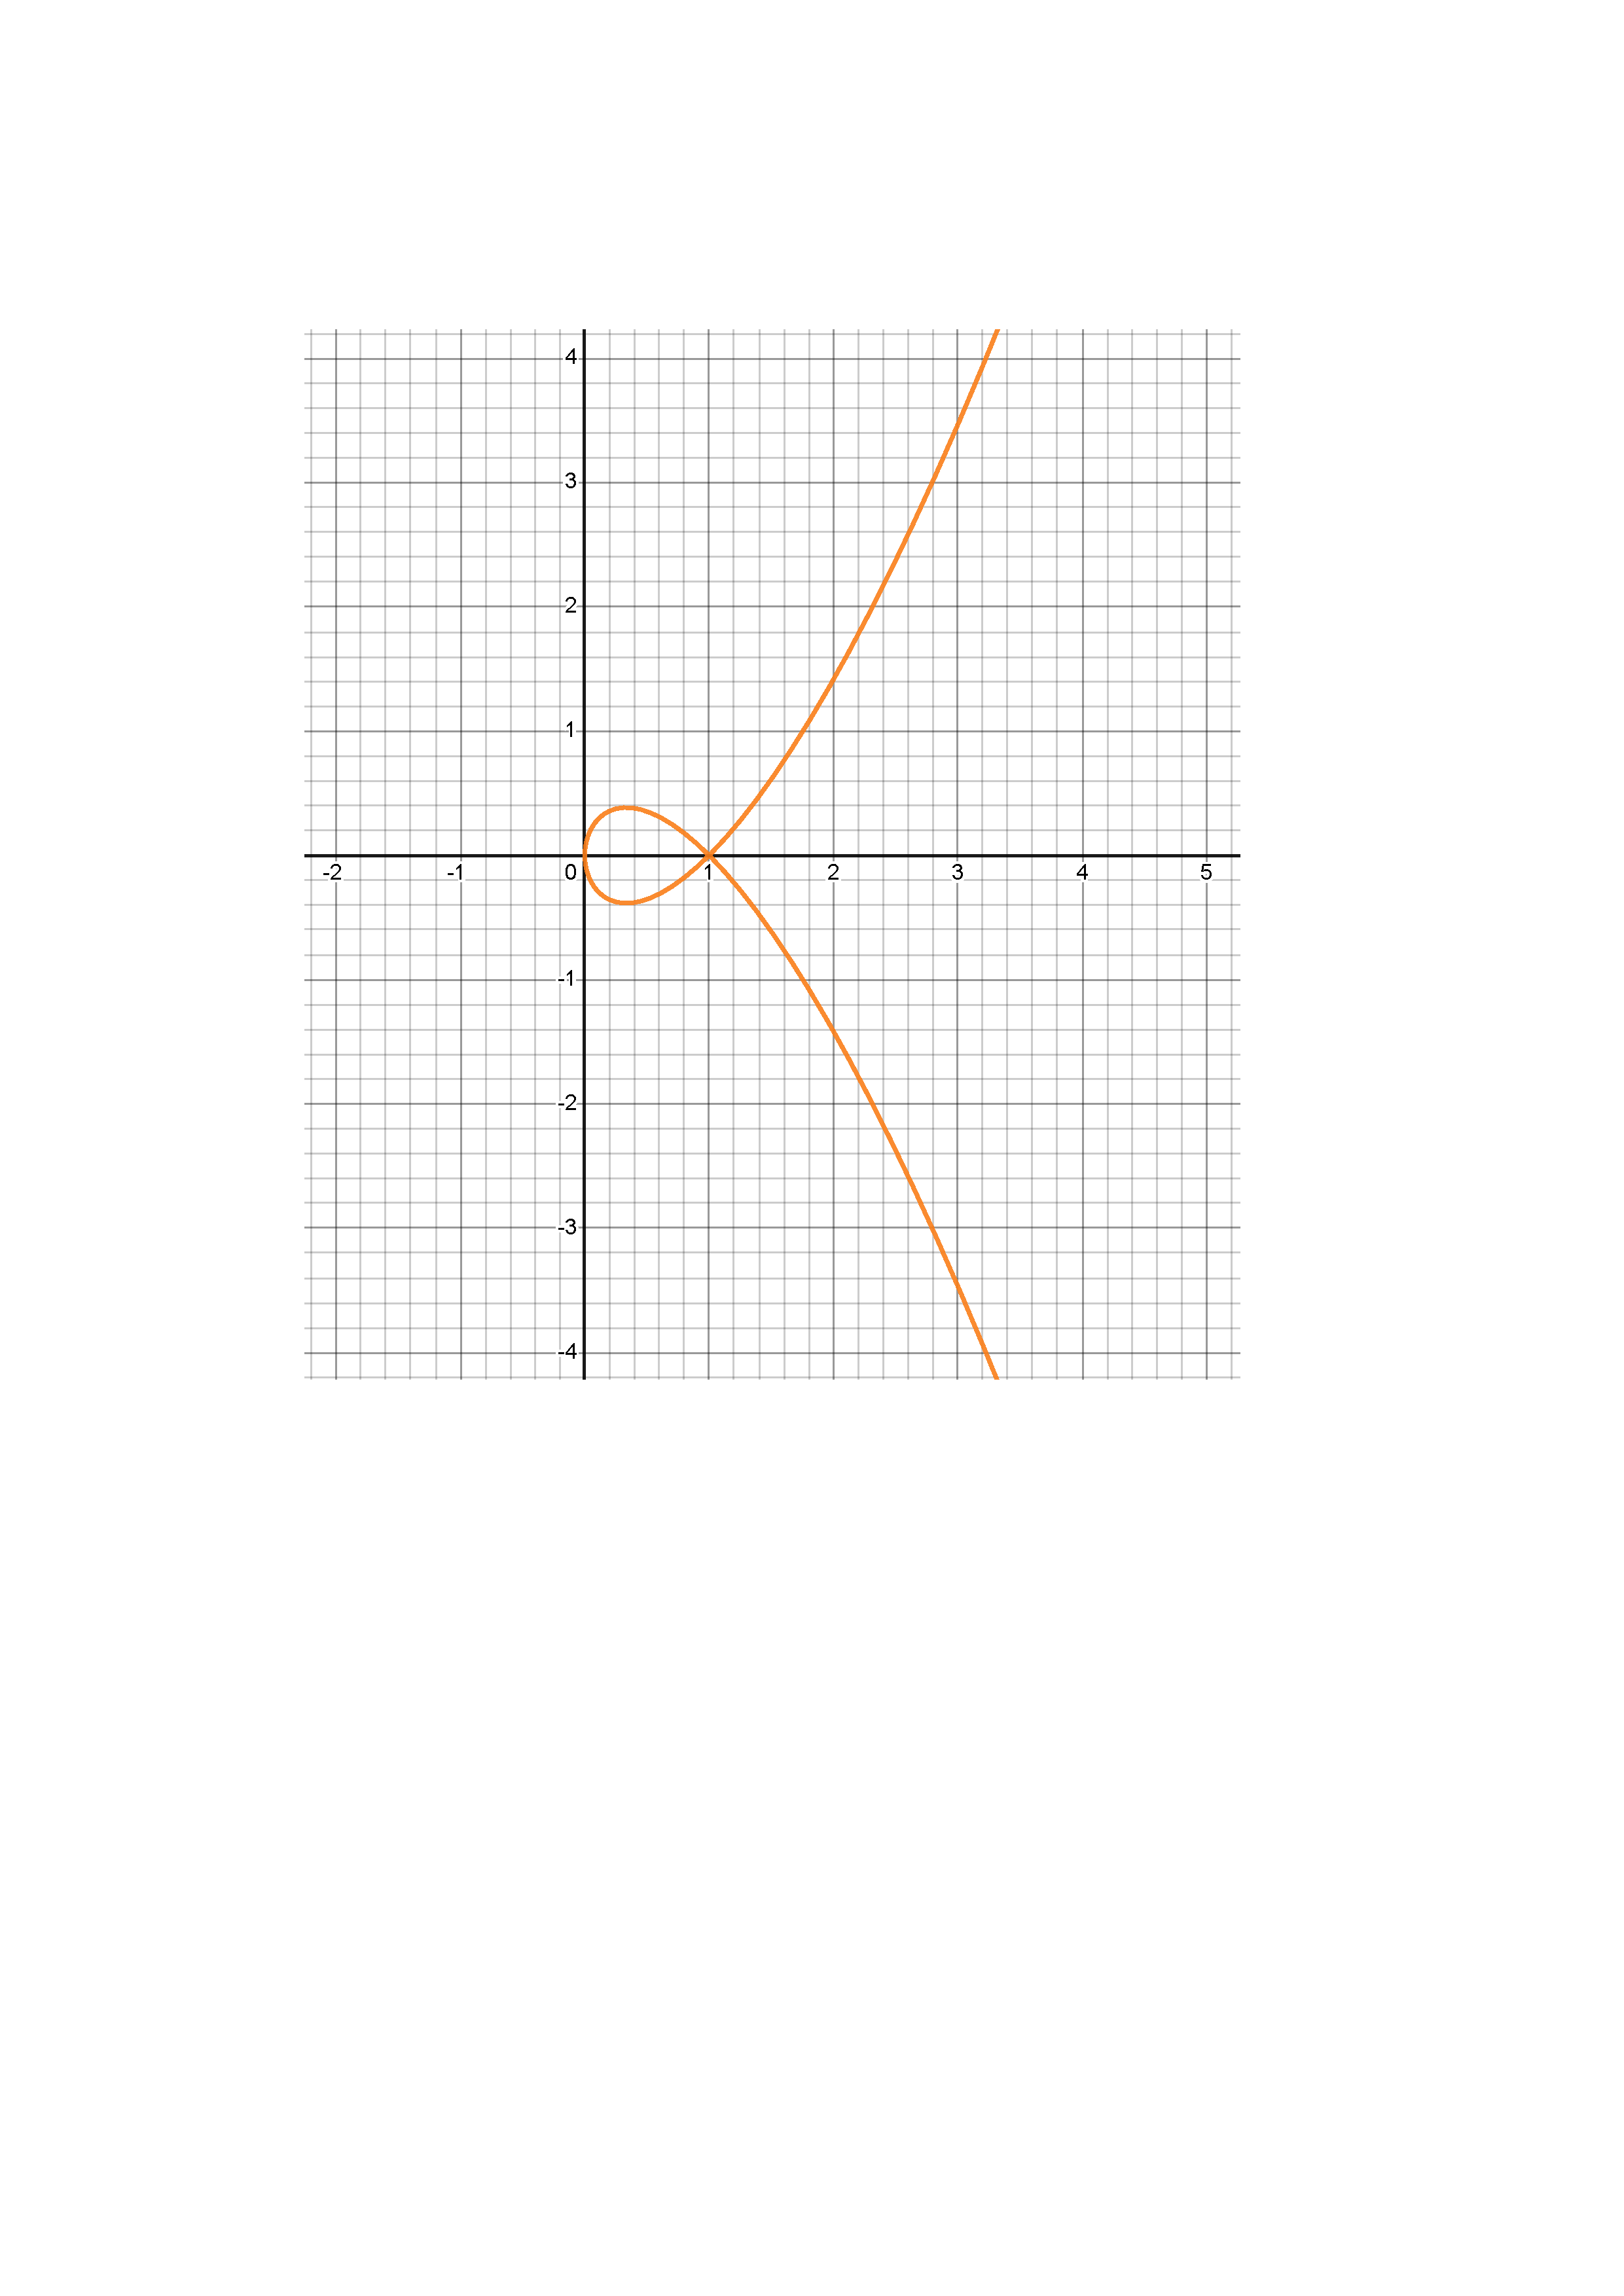
\includegraphics[width=.8\textwidth]{img/parametrizzazioni-3.pdf}
		\caption*{$\gamma: \mathbb{R} \rightarrow \mathbb{R}^{2} \hspace{2em} t\mapsto\left(t^{2}, t^{3}-t\right)$ è una curva non semplice.}
	\end{figure}\newpage

	\subsubsection{Parametrizzazioni notevoli}\label{subsubsection: parametrizzazioni notevoli}

	Esistono tre tipi di parametrizzazioni notevoli: per un segmento, per un grafico di una funzione e per le coniche.

	\begin{flushleft}\label{parametrizzazione notevole: segmento}
		\definition{Parametrizzazione notevole: \underline{segmento}}
	\end{flushleft}
	Dato il seguente grafico:
	\begin{figure}[!htp]
		\centering
		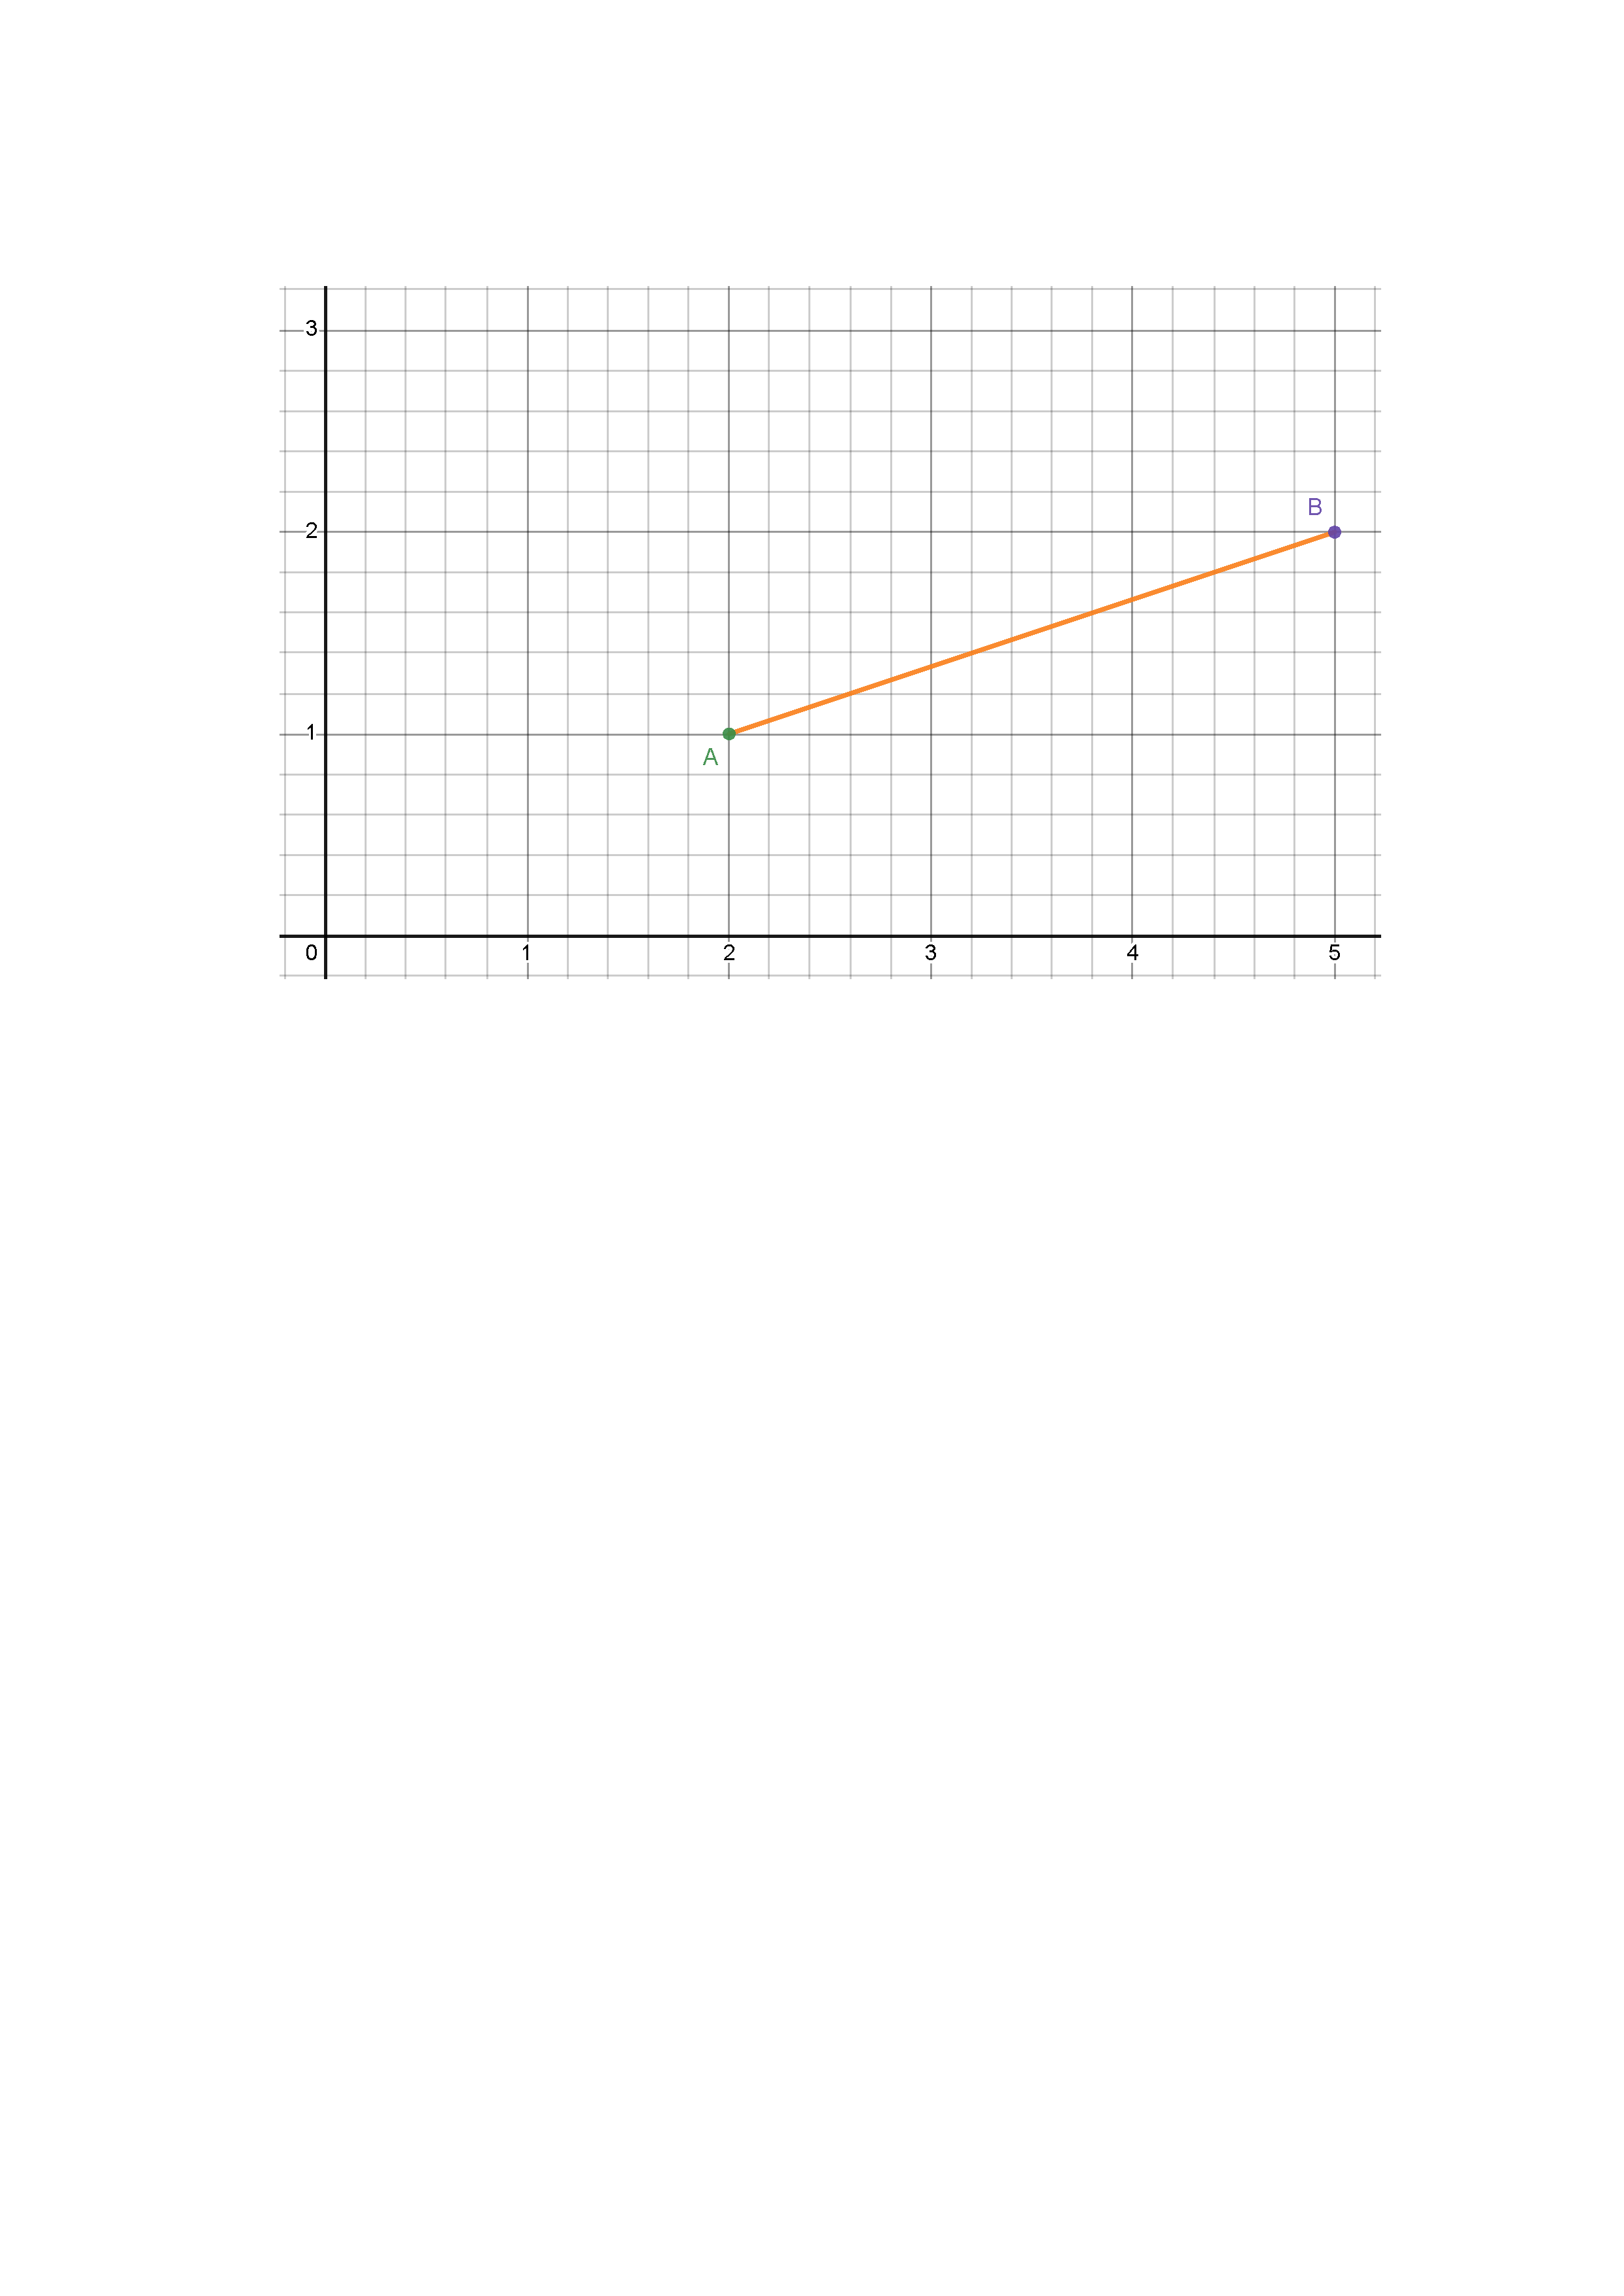
\includegraphics[width=.8\textwidth]{img/parametrizzazioni_notevoli-1.pdf}
	\end{figure}

	\noindent
	Si definisce il vettore $\overrightarrow{v}$ che parte dal punto $B$ e finisce al punto $A$ come:
	\begin{equation*}
		\overrightarrow{v} = B - A = \left(5,2\right) - \left(2,1\right) = \left(3,1\right)
	\end{equation*}
	La \textbf{parametrizzazione notevole} di una retta (segmento) è la seguente formula:
	\begin{equation}\label{eq: parametrizzazione notevole: segmento o retta}
		\gamma\left(t\right) = A + t \cdot \overrightarrow{v} \hspace{2em} \text{con } t \in \left[0,1\right]
	\end{equation}
	Sostituendo i valori noti in questo esempio:
	\begin{equation*}
		\gamma\left(t\right) = \left(2,1\right) + t\left(3,1\right) = \left(2 + 3t, 1 + t\right)
	\end{equation*}
	La parametrizzazione dunque è:
	\begin{equation*}
		\begin{array}{rcl}
			\gamma : \left[0,1\right] &\rightarrow& \mathbb{R}^{2} \\
			t &\mapsto& \left(2+3t, 1+t\right)
		\end{array}
	\end{equation*}\newpage

	\begin{flushleft}
		\definition{Parametrizzazione notevole: \underline{grafico di una funzione}}
	\end{flushleft}
	Dato il seguente grafico come esempio:
	\begin{figure}[!htp]
		\centering
		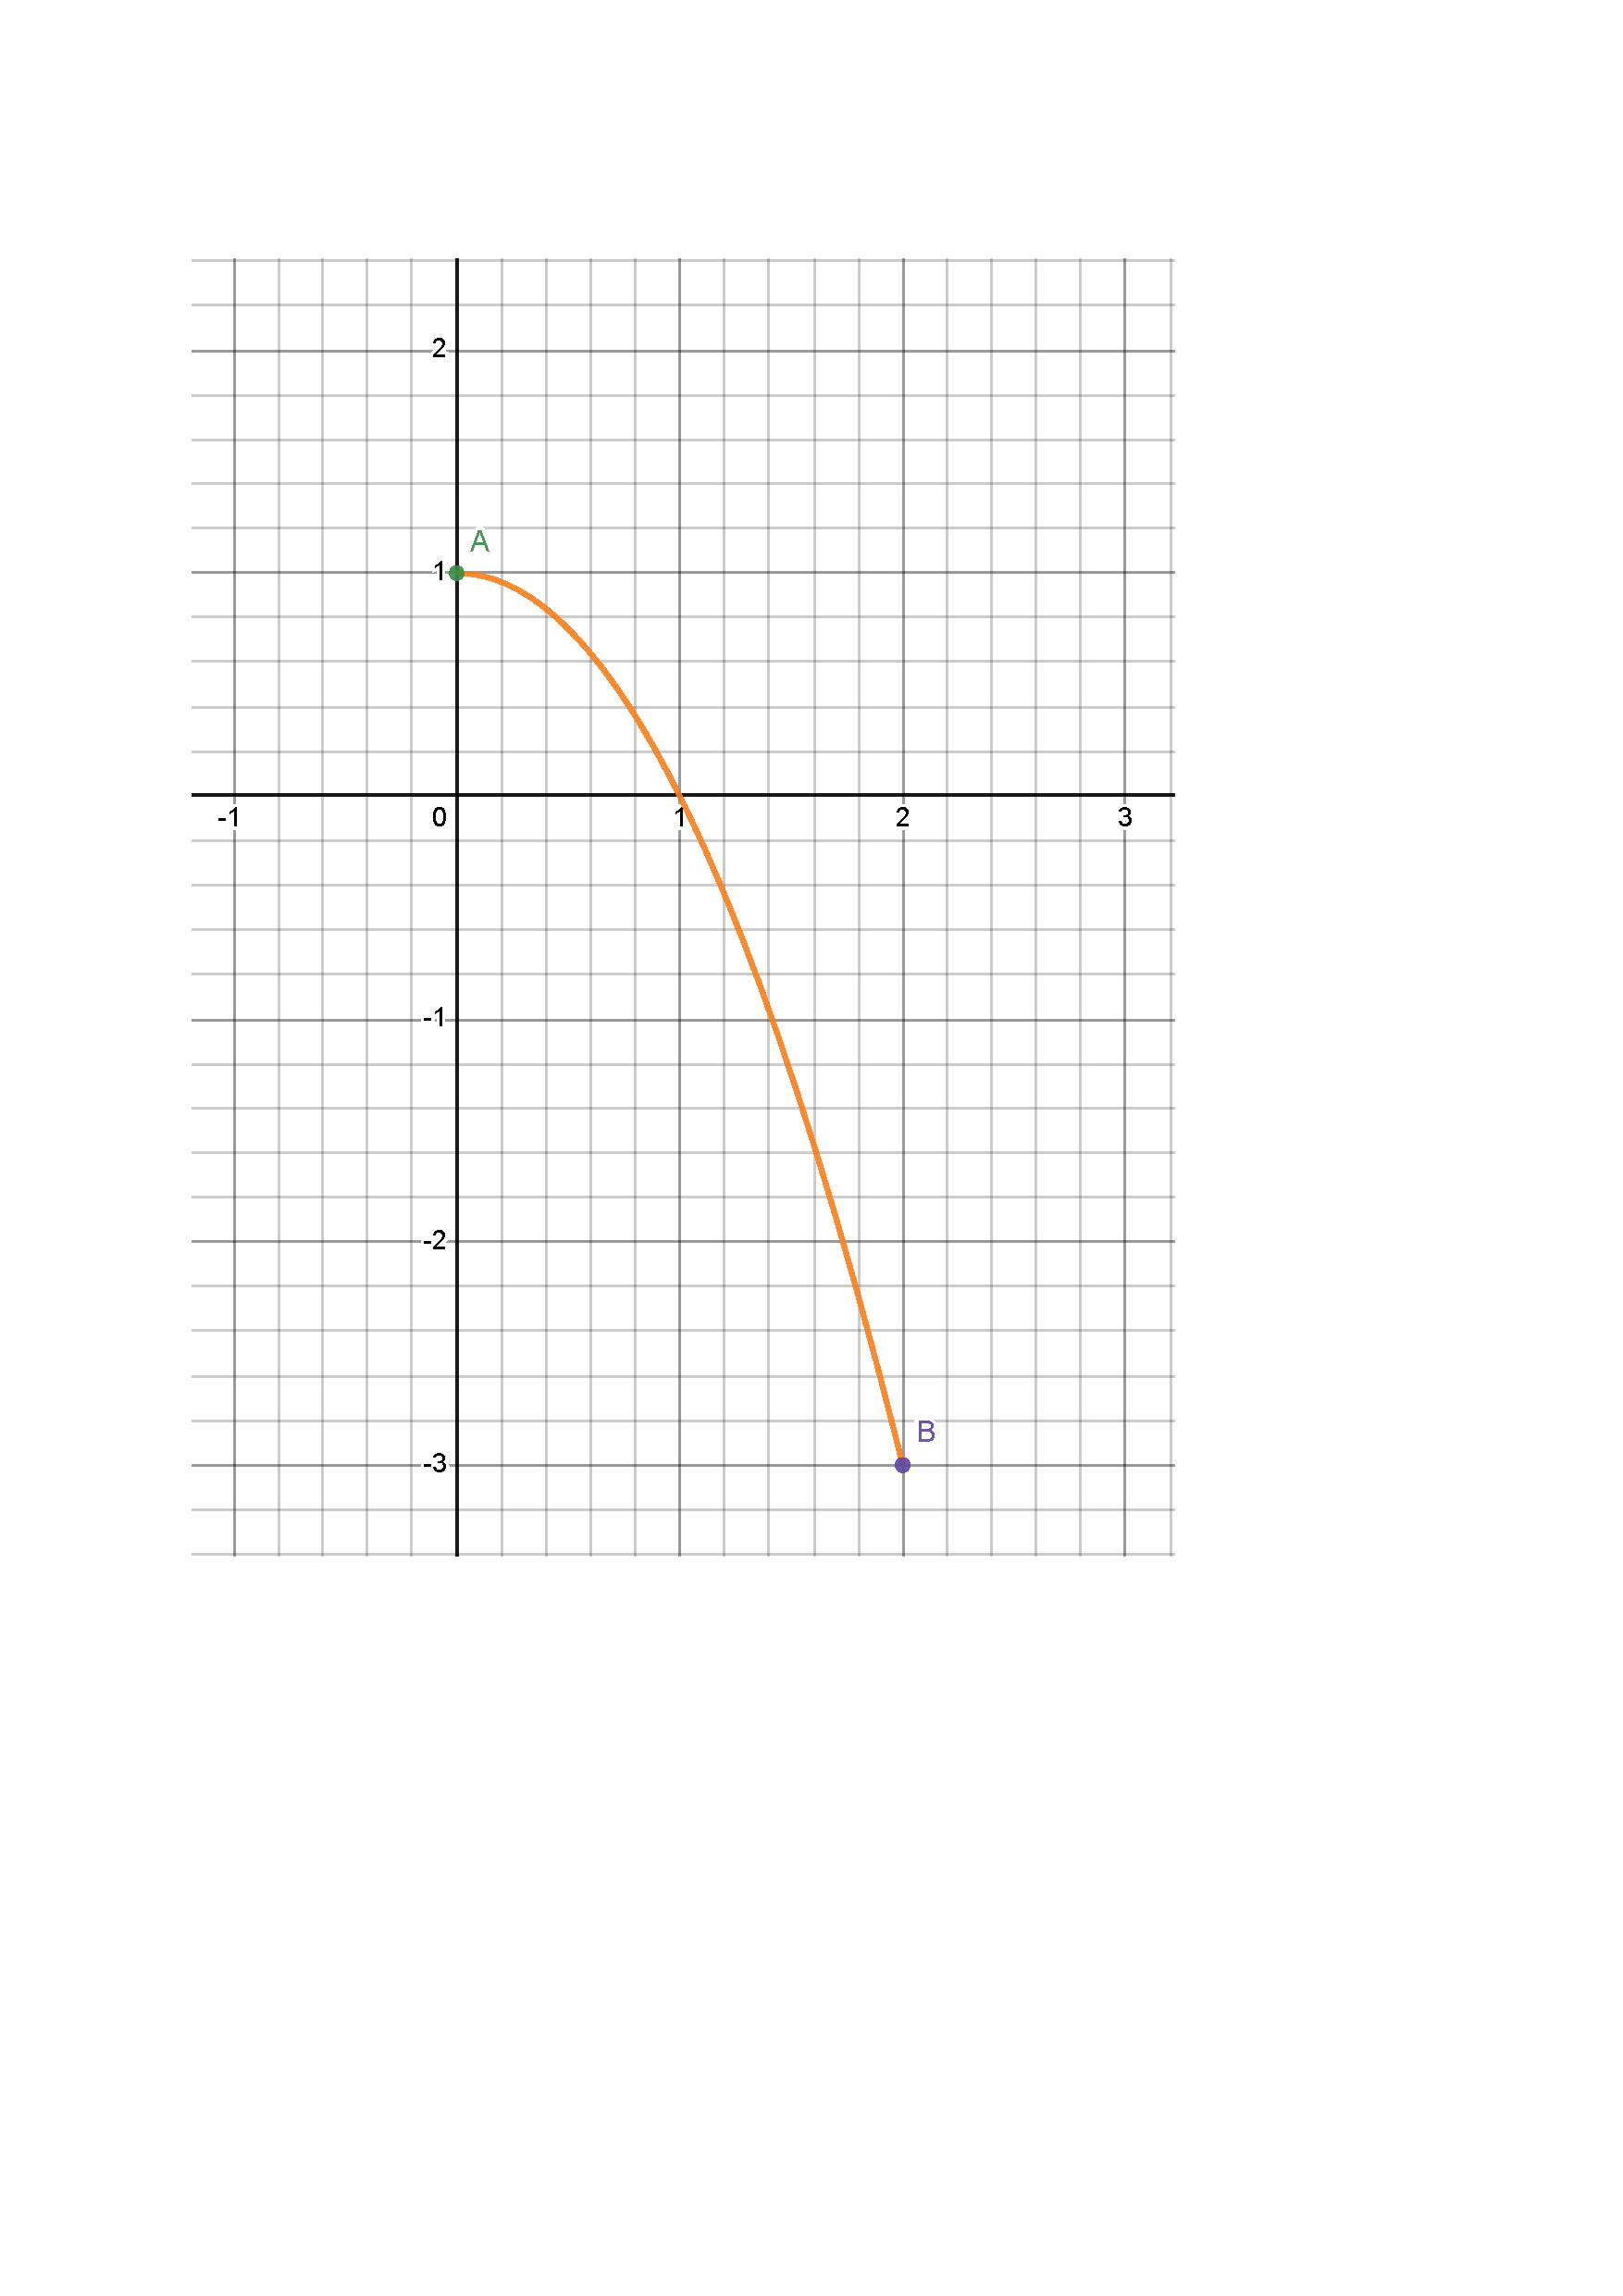
\includegraphics[width=.55\textwidth]{img/parametrizzazioni_notevoli-2.pdf}
	\end{figure}

	\noindent
	Il grafico di una funzione:
	\begin{equation*}
		\begin{array}{rcl}
			f : I &\rightarrow& \mathbb{R} \\
			x &\mapsto& f\left(x\right)
		\end{array}
	\end{equation*}
	Ha una parametrizzazione del tipo:
	\begin{equation}
		\begin{array}{rcl}
			\gamma : I &\rightarrow& \mathbb{R}^{2} \\
			t &\mapsto& \left(t, f\left(t\right)\right)
		\end{array}
	\end{equation}
	L'esempio ha i punti $A = \left(0,1\right)$ e $B = \left(2,-3\right)$ e dunque la parametrizzazione è:
	\begin{equation*}
		\begin{array}{rcl}
			\gamma\left[0,2\right] &\rightarrow& \mathbb{R}^{2} \\
			t &\mapsto& \left(t, 1-t^{2}\right)
		\end{array}
	\end{equation*}

	\begin{flushleft}
		\definition{Parametrizzazione notevole: \underline{conica}}
	\end{flushleft}
	\begin{itemize}
		\item La parametrizzazione di un'\textbf{ellisse di centro} $\left(x_{c}, y_{c}\right)$ e semiassi $a,b$:
		\begin{equation*}
			\begin{array}{rcl}
				\gamma:\left[0,2\pi\right] &\rightarrow& \mathbb{R}^{2} \\
				t &\mapsto& \left(x_{c} + a \cos\left(t\right), y_{c} + b \sin\left(t\right)\right)
			\end{array}
		\end{equation*}

		\item La parametrizzazione dell'\textbf{iperbole equilatera} $\left(x^{2}-y^{2} = 1, \: x > 0\right)$:
		\begin{equation*}
			\begin{array}{rcl}
				\mathbb{R} &\rightarrow& \mathbb{R}^{2} \\
				t &\mapsto& \left(\cosh\left(t\right), \sinh\left(t\right)\right)
			\end{array}
		\end{equation*}
		Ricordando che $\cosh\left(t\right) = \dfrac{e^{t} + e^{-t}}{2}$ e $\sinh\left(t\right) = \dfrac{e^{t} - e^{-t}}{2}$
	\end{itemize}\newpage

	\subsubsection{Retta tangente a una curva}\label{subsubsection: retta tangente a una curva}

	Una curva $\gamma\left(t\right)$, con $t \in I$, è derivabile in $I$ se e solo se tutte le sue componenti sono derivabili in $I$ e in tal caso:
	\begin{equation*}
		\gamma'\left(t\right) = \left(\gamma_{1}'\left(t\right), \gamma_{2}'\left(t\right), \cdots, \gamma_{n}'\left(t\right)\right)
	\end{equation*}
	Si può interpretare la derivata della curva $\gamma'\left(t\right)$ come un vettore velocità di un punto, il quale descrive la traiettoria (sostegno della curva $\gamma$) secondo la parametrizzazione data.

	Nel caso in cui la derivata è diversa dal vettore zero, $\gamma'\left(t_{0}\right) \ne \overrightarrow{0}$, allora una \definition{parametrizzazione della retta tangente alla curva} in $\gamma\left(t_{0}\right)$ è:
	\begin{equation}\label{eq: parametrizzazione della retta tangente alla curva}
		r\left(t\right) = \gamma\left(t_{0}\right) + t\gamma'\left(t_{0}\right) \hspace{2em} t \in \mathbb{R}
	\end{equation}

	\longline

	\subsubsection{Esercizio parametrizzazione retta tangente}\label{subsubsection: esercizio parametrizzazione retta tangente}
	
	Trovare l'equazione della retta tangente al sostegno della curva:
	\begin{equation*}
		\begin{array}{rcl}
			\gamma:\left(-1, +\infty\right) &\rightarrow& \mathbb{R}^{3} \\
			t &\mapsto& \left(e^{t}, \ln\left(t+1\right), t\right)
		\end{array}
	\end{equation*}
	Nel suo punto di coordinate $\left(1, 0, 0\right)$. Il \textbf{primo passo} è trovare un punto $t_{0}$ appartenente alla curva $\left(-1,+\infty\right)$ tale che il risultato sia $\gamma\left(t_{0}\right) = \left(1,0,0\right)$. Per questo motivo, si inseriscono i valori nel sistema:
	\begin{equation*}
		\begin{cases}
			e^{t} = 1 \\
			\ln\left(t+1\right) = 0 \\
			t = 0
		\end{cases}
		\xrightarrow{\text{soluzione immediata}}
		t_{0} = 0
	\end{equation*}
	Il \textbf{secondo passo} è calcolare la derivata in quel punto:
	\begin{equation*}
		\left. \gamma'\left(t\right) \right|_{t = 0} 
		=
		\left. 
		\begin{cases}
			\frac{d}{dt} \left(e^{t}\right) \\
			\frac{d}{dt} \left(\ln\left(t+1\right)\right) \\
			\frac{d}{dt} \left(t\right)
		\end{cases} 
		\right|_{t=0}
		=
		\left.
		\begin{cases}
			e^{t} \\
			\frac{1}{t+1} \\
			1
		\end{cases}
		\right|_{t=0}
		=
		\left(1,1,1\right)
	\end{equation*}
	Il \textbf{terzo e ultimo passo} è scrivere l'equazione della tangente (eq. \ref{eq: parametrizzazione della retta tangente alla curva}):
	\begin{equation*}
		r\left(s\right) = \gamma\left(t_{0}\right) + s \cdot \gamma'\left(t_{0}\right) = \left(1,0,0\right) + s\left(1,1,1\right) = \left(1+s, s, s\right)
	\end{equation*}
	Questa risulta essere l'equazione parametrica:
	\begin{equation*}
		\begin{cases}
			x = 1+s \\
			y = s \\
			z = s
		\end{cases}
		\hspace{1em}
		s \in \mathbb{R}
	\end{equation*}\newpage

	\subsubsection{Esercizio parametrizzazione arco di ellisse}\label{subsubsection: esercizio parametrizzazione arco di ellisse}
	
	Trovare una parametrizzazione dell'arco di ellisse di equazione:
	\begin{equation*}
		4x^{2} + 9y^{2} + 8x - 36y + 4 = 0
	\end{equation*}
	E si scriva poi l'equazione della tangente alla curva in $P\left(-1 - \dfrac{3\sqrt{3}}{2}, +1\right)$.
	
	\noindent
	Il \textbf{primo passo} è verificare che l'equazione data sia in forma canonica e in caso contrario ottenerla con le varie tecniche introdotte nel capitolo dei Prerequisiti. Quindi, si esegue la tecnica del completamento dei quadrati (par. \ref{subsubsection: completamento dei quadrati}) per ottenere la forma canonica:
	\begin{itemize}
		\item Si raggruppano le variabili:
		\begin{equation*}
			4\left(x^{2} + 2x\right) + 9\left(y^{2} - 4y\right) + 4 = 0
		\end{equation*}

		\item Si cerca un $\Delta = 0$:
		\begin{equation*}
			\begin{array}{rcl}
				x^{2} + 2x &\rightarrow& 2^{2} - 4 \cdot 1 \cdot c = 0 \\ [.3em]
									  && -4c = -4 \\ [.3em]
									  && c = 1 \\ [1em]
				y^{2} - 4y &\rightarrow& \left(-4\right)^{2} - 4 \cdot 1 \cdot c = 0 \\ [.3em]
									  && -4c = -16 \\ [.3em]
									  && c = 4
			\end{array}
		\end{equation*}

		\item Si riscrive l'equazione:
		\begin{equation*}
			4\left(x^{2} + 2x + 1 - 1\right) + 9\left(y^{2} - 4y + 4 - 4\right) + 4 = 0
		\end{equation*}

		\item Si raggruppano le equazioni di secondo grado con i nuovi termini e si ottiene l'equazione canonica:
		\begin{gather*}
			\begin{array}{rcl}
				x^{2} + 2x + 1 &\rightarrow& \dfrac{-2 \pm 0}{2 \cdot 1} = -1 \\ [1em]
				y^{2} - 4y + 4 &\rightarrow& \dfrac{-\left(-4\right) \pm 0}{2 \cdot 1} = 2
			\end{array}
			\\ \\
			\begin{array}{rcl}
				4\left(\left(x+1\right)^{2} - 1\right) + 9\left(\left(y-2\right)^{2} - 4\right) + 4 &=& 0 \\ [1em]
				4\left(x+1\right)^{2} - 4 + 9\left(y-2\right)^{2} - 36 + 4 &=& 0 \\ [1em]
				4\left(x+1\right)^{2} + 9\left(y-2\right)^{2} &=& 36 \\ [1em]
				\dfrac{1}{36} \cdot 4\left(x+1\right)^{2} + \dfrac{1}{36} \cdot 9\left(y-2\right)^{2} &=& 36 \cdot \dfrac{1}{36} \\ [1em]
				\dfrac{\left(x+1\right)^{2}}{9} + \dfrac{\left(y-2\right)^{2}}{4} &=& 1
			\end{array}
		\end{gather*}
	\end{itemize}
	La parametrizzazione di un'ellisse di centro $\left(x_{c}, y_{c}\right)$ e semiassi $a,b$ è:
	\begin{equation*}
		\gamma:\left[0,2\pi\right] \rightarrow \mathbb{R}^{2} \hspace{2em}
		t 
		\mapsto 
		\begin{cases}
			x_{c} + a \cos\left(t\right) \\
			y_{c} + b \sin\left(t\right)
		\end{cases}
	\end{equation*}
	Quindi, il \textbf{secondo passo} è trovare la parametrizzazione. In questo esempio, l'ellisse è centrata in $\left(-1, 2\right)$ mentre i semiassi sono $a = \sqrt{9} = 3$ e $b = \sqrt{4} = 2$. Per cui, la parametrizzazione di un'ellisse è:
	\begin{equation*}
		\gamma:\left[0,2\pi\right] \rightarrow \mathbb{R}^{2} \hspace{2em}
		t 
		\mapsto 
		\begin{cases}
			-1 + 3 \cos\left(t\right) \\
			2  + 2 \sin\left(t\right)
		\end{cases}
	\end{equation*}
	Il \textbf{terzo passo} è eguagliare la parametrizzazione al punto $P$ questo perché è necessario trovare l'equazione della tangente alla curva. Per questo motivo, si procede il calcolo con il sistema:
	\begin{equation*}
		\begin{cases}
			-1 + 3 \cos\left(t\right) = -1 - \dfrac{3\sqrt{3}}{2} \\
			2  + 2 \sin\left(t\right) = +1
		\end{cases}
		\rightarrow
		\begin{cases}
			\cos\left(t\right) = - \dfrac{3\sqrt{3}}{2} \cdot \dfrac{1}{3} \\
			\\
			\sin\left(t\right) = -1 \cdot \dfrac{1}{2}
		\end{cases}
		\rightarrow
		\begin{cases}
			\cos\left(t\right) = - \dfrac{\sqrt{3}}{2} \\
			\\
			\sin\left(t\right) = - \dfrac{1}{2}
		\end{cases}
	\end{equation*}
	A questo punto il calcolo della $t$ non è banale perché applicando la funzione $\arccos$ e $\arcsin$, si otterrebbero due valori differenti di $t$. Quindi come è possibile ottenerla? Si utilizza la definizione di tangente che è seno fratto coseno:
	\begin{equation*}
		\tan\left(t\right) = \dfrac{\sin\left(t\right)}{\cos\left(t\right)} \rightarrow \tan\left(t\right) = \dfrac{-\frac{1}{2}}{-\frac{\sqrt{3}}{2}} = -\dfrac{1}{2} \div -\dfrac{\sqrt{3}}{2} = -\dfrac{1}{2} \cdot -\dfrac{2}{\sqrt{3}} = \dfrac{1}{\sqrt{3}}
	\end{equation*}
	Con l'arcotangente si ottiene il valore $t$:
	\begin{equation*}
		\arctan\left(\dfrac{1}{\sqrt{3}}\right) = t = \dfrac{\pi}{6}
	\end{equation*}
	Ma attenzione! Con $\frac{\pi}{6}$ il valore del coseno e seno sarebbero differenti (riguardo il segno). Questo perché, la funzione arcotangente restituisce il primo valore trovato, ovvero quello nel quadrante positivo (si veda la figura \ref{fig: funzione tan} nella pagina successiva).
	
	Per risolvere questo problema, si disegna una circonferenza su un piano cartesiano, e partendo dal punto $\left(1,0\right)$, si cerca, con i diversi livelli di gradi, di arrivare nel quadrante interessato. Quindi:
	\begin{itemize}
		\item Il primo quadrante (in alto a dx) avrà i valori del seno e coseno positivi. Il range dei gradi è: $\left(0\degree,90\degree\right)$
		\item Il secondo quadrante (in alto a sx) avrà i valori del coseno negativi e del seno positivi. Il range dei gradi è: $\left(90\degree, 180\degree\right)$
		\item Il terzo quadrante (in basso a sx) avrà i valori del coseno e del seno negativi. Il range dei gradi è: $\left(180\degree, 270\degree\right)$
		\item Il quarto quadrante (in basso a dx) avrà i valori del coseno positivi e i valori del seno negativi. Il range dei gradi è: $\left(270\degree, 0\degree\right)$
	\end{itemize}\newpage
	\begin{figure}[!htp]
		\centering
		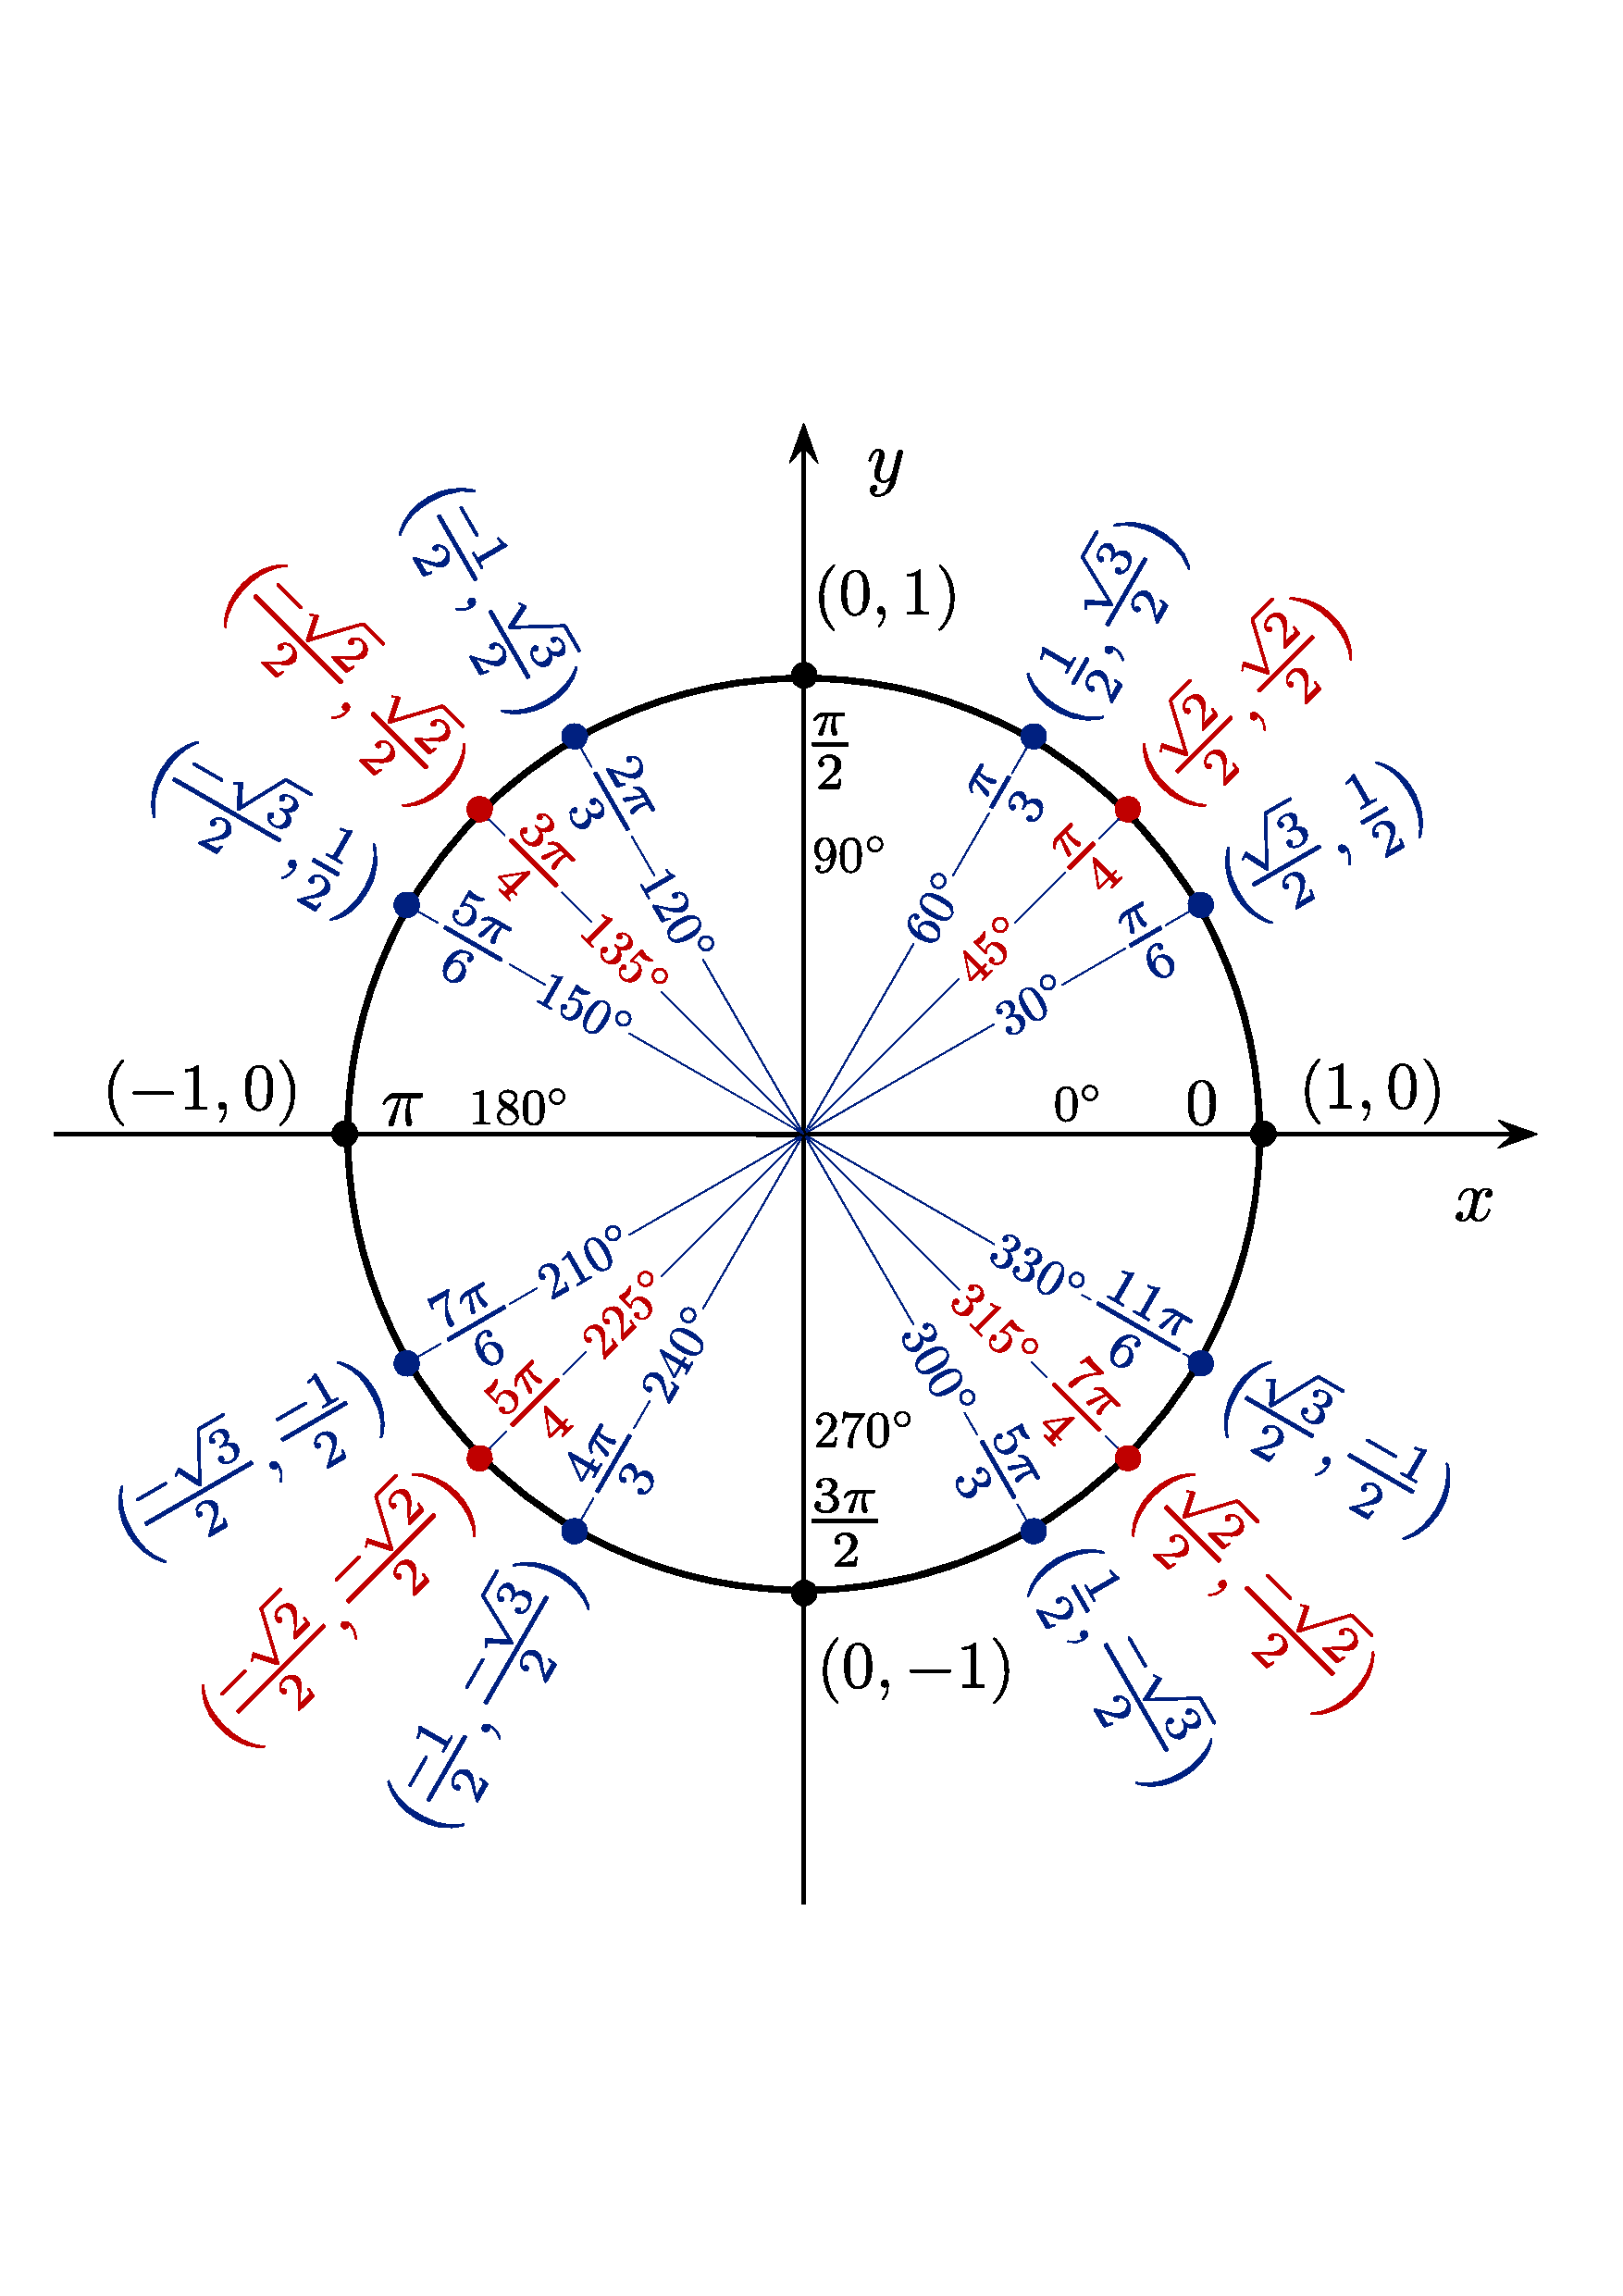
\includegraphics[width=.7\textwidth]{img/trigonometria_tan.pdf}
		\caption{I valori assunti dalla funzione $\tan$.}
		\label{fig: funzione tan}
	\end{figure}
	
	\noindent
	Portando il valore $\frac{\pi}{6}$ da radianti a gradi (ricordando $\pi = 180\degree$, quindi $\frac{1}{6}\pi = \frac{1}{6} \cdot 180 = 30\degree$) si ottengono $30\degree$. Quindi, sapendo che il terzo quadrante è quello interessato, per arrivarci si continua ad aumentare il valore stesso:
	\begin{gather*}
		\begin{array}{rcl}
			30\degree+30\degree+30\degree=90\degree &\rightarrow& \text{primo quadrante passato} \\
			90\degree+30\degree+30\degree+30\degree=180\degree &\rightarrow& \text{secondo quadrante passato} \\
			180\degree+30\degree = 210\degree &\rightarrow& \text{primo valore ammesso nel terzo quadrante}
		\end{array}
	\end{gather*}
	Il valore è stato aumentato $7$ volte, per cui, al valore $\frac{\pi}{6}$ (corrispondente valore in radianti di $30\degree$) basterà moltiplicare $7$:
	\begin{equation*}
		t = \dfrac{7\pi}{6}
	\end{equation*}

	\noindent
	Come viene mostrata nell'equazione \ref{eq: parametrizzazione della retta tangente alla curva}, per ottenere l'equazione è necessaria la derivata della parametrizzazione. Per cui, il \textbf{quarto passo} è eseguire la derivata della parametrizzazione e valutarla nel valore $t$ trovato con il punto $P$ nel passaggio precedente:
	\begin{equation*}
		\gamma'\left(t\right) = \begin{cases}
			-3\sin\left(t\right) \\
			2\cos\left(t\right)
		\end{cases}
		\rightarrow
		\gamma'\left(\dfrac{7\pi}{6}\right) = \begin{cases}
			-3\sin\left(\dfrac{7\pi}{6}\right) \\ \\
			2\cos\left(\dfrac{7\pi}{6}\right)
		\end{cases} = \begin{cases}
			\dfrac{3}{2} \\ \\
			-\sqrt{3}
		\end{cases}
	\end{equation*}\newpage

	\noindent
	Il \textbf{quinto passo} è applicare l'equazione \ref{eq: parametrizzazione della retta tangente alla curva}:
	\begin{equation*}
		\begin{array}{rcl}
			r\left(t\right) &=& \gamma\left(t\right) + t \cdot \gamma'\left(t\right) \hspace{2em} t \in \mathbb{R} \\ [1em]
			%
			&=& \begin{cases}
				-1 + 3 \cos\left(\dfrac{7\pi}{6}\right) \\
				\\
				2  + 2 \sin\left(\dfrac{7\pi}{6}\right)
			\end{cases}
			+
			t \cdot
			\begin{cases}
				-3\sin\left(\dfrac{7\pi}{6}\right) \\ \\
				2\cos\left(\dfrac{7\pi}{6}\right)
			\end{cases} \\ [3.5em]
			%
			&=& 
			\begin{cases}
				-1-\dfrac{3\sqrt{3}}{2} \\
				1
			\end{cases}
			+
			t \cdot
			\begin{cases}
				\dfrac{3}{2} \\ \\
				-\sqrt{3}
			\end{cases} \\ [3em]
			%
			&=&
			\begin{cases}
				-1-\dfrac{3\sqrt{3}}{2} + \dfrac{3}{2}t \\ \\
				1 - \sqrt{3} t
			\end{cases}
			\hspace{2em}
			t \in \mathbb{R}
		\end{array}
	\end{equation*}
	L'esercizio si conclude qua con l'equazione della retta tangente.\newpage

	\subsubsection{Lunghezza di una curva}\label{subsubsection: lunghezza di una curva}

	Dato l'arco di curva:
	\begin{equation*}
		\gamma:\left[a,b\right] \rightarrow \mathbb{R}^{n}
	\end{equation*}
	E una partizione dell'intervallo $\left[a,b\right]$:
	\begin{equation*}
		\mathcal{P} = \left\{a=t_{0}, t_{1}, t_{2}, \cdots, b = t_{m}\right\}
	\end{equation*}
	Alla partizione rimane associata una poligonale, di cui si può \textbf{calcolare la lunghezza} (di una curva):
	\begin{equation}\label{eq: lunghezza di una curva}
		L\left(\mathcal{P}\right) = \displaystyle\sum_{i=1}^{m} \left|\left| \gamma\left(t_{i}\right) - \gamma \left(t_{i-1}\right) \right|\right|
	\end{equation}

	\begin{boxdef}
		Si dice che un \definition{arco di curva} è \definition{rettificabile} se $\sup_{\mathcal{P}} L\left(\mathcal{P} < \infty\right)$. In tal caso, per definizione:
		\begin{equation*}
			L\left(\gamma\right) = \sup_{\mathcal{P}} L\left(\mathcal{P}\right)
		\end{equation*}
	\end{boxdef}

	\begin{boxdef}
		Se $\gamma : \left[a,b\right] \rightarrow \mathbb{R}^{n}$ è un arco di curva regolare, ovvero la derivata prima è diverso al vettore nullo ed è continua, allora è rettificabile e la sua \definition{lunghezza} è:
		\begin{equation}
			\displaystyle\int_{a}^{b} \left|\left| \gamma'\left(t\right) \right|\right| \: \mathrm{d}t
		\end{equation}
	\end{boxdef}

	\noindent
	Dove la lunghezza viene calcolata in questo modo:
	\begin{equation}\label{eq: lunghezza di una curva}
		\left|\left| \gamma'\left(t\right) \right|\right| = \sqrt{x^{2} + y^{2} + \cdots n^{2}}
	\end{equation}
	In cui tutte le variabili sotto radice sono i valori della parametrizzazione. Ovviamente devono essere inseriti post derivata. Si veda gli esempi.

	\begin{flushleft}
		\example{\underline{Esempio 1}}
	\end{flushleft}
	Calcolare la lunghezza dell'arco di curva:
	\begin{equation*}
		\begin{array}{rcl}
			\gamma:\left[0,2\pi\right] &\rightarrow& \mathbb{R}^{3} \\
			t &\mapsto& \left(\cos\left(t\right), \sin\left(t\right), 3t\right)
		\end{array}
	\end{equation*}
	Il \textbf{primo passo} per calcolare la lunghezza è trovare la derivata:
	\begin{equation*}
		\gamma'\left(t\right) = \begin{cases}
			-\sin\left(t\right) \\
			\cos\left(t\right) \\
			3
		\end{cases}
	\end{equation*}
	Il \textbf{secondo passo} è calcolare l'integrale applicando l'equazione \ref{eq: lunghezza di una curva}:
	\begin{equation*}
		\displaystyle\int_{0}^{2\pi} \sqrt{\left(-\sin\left(t\right)\right)^{2} + \left(\cos\left(t\right)\right)^{2} + \left(3\right)^{2}} \:\mathrm{d}t = \displaystyle\int_{0}^{2\pi} \sqrt{10} \:\mathrm{d}t = \left[\sqrt{10}t\right]_{0}^{2\pi} = \sqrt{10} \cdot 2\pi
	\end{equation*}\newpage


	\newpage
	\newpage
	\newpage
	\subsection{Esercizi}

	\subsubsection{Limiti e continuità}

	\begin{flushleft}\label{exam: esame 01 marzo 2022 - Gruppo A - 4 esercizio}
		\definition{\underline{Esame 1 marzo 2022 - Gruppo A}}
	\end{flushleft}
	\example{\emph{Stabilire se la funzione}
	\begin{equation*}
		f\left(x,y\right) = \begin{cases}
			\dfrac{\left(x-1\right)\left(y-2\right)}{\sqrt{\left(x-1\right)^{2} + \left(y-2\right)^{2}}} & \left(x,y\right) \ne \left(1,2\right) \\
			\\
			0 & \left(x,y\right) = \left(1,2\right)
		\end{cases}
	\end{equation*}
	\emph{è continua in $\mathbb{R}^{2}$.}}
	
	\noindent
	\example{\emph{Se sostituiamo l'espressione $\sqrt{\left(x-1\right)^{2} + \left(y-2\right)^{2}}$ con $\left(x-1\right)^{2} + \left(y-2\right)^{2}$, la risposta cambia?}}\newline

	\noindent
	Vedendo i termini al denominatore (al quadrato) e i punti $a,b$, cioè $1,2$, si può tentare di utilizzare le coordinate polari così da avere una semplificazione, non da poco, al denominatore. Quindi, le coordinate polari sono:
	\begin{equation*}
		\begin{cases}
			x = 1 + r\cos\left(\theta\right) \\
			y = 2 + r\sin\left(\theta\right)
		\end{cases}
	\end{equation*}
	Si sostituiscono le coordinate polari nell'espressione:
	\begin{equation*}
		\dfrac{\left(x-1\right)\left(y-2\right)}{\sqrt{\left(x-1\right)^{2} + \left(y-2\right)^{2}}} 
		\rightarrow
		\dfrac{
			\left(1 + r\cos\left(\theta\right)-1\right)\left(2 + r\sin\left(\theta\right)-2\right)
		}{
			\sqrt{\left(1 + r\cos\left(\theta\right)-1\right)^{2} + \left(2 + r\sin\left(\theta\right)-2\right)^{2}}
		}
	\end{equation*}
	Si eseguono alcune manipolazioni algebriche:
	\begin{equation*}
		\begin{array}{rcl}
			\dfrac{
				\left(1 + r\cos\left(\theta\right)-1\right)\left(2 + r\sin\left(\theta\right)-2\right)
			}{
				\sqrt{\left(1 + r\cos\left(\theta\right)-1\right)^{2} + \left(2 + r\sin\left(\theta\right)-2\right)^{2}}
			}
			&=&
			\dfrac{
				\left(r\cos\left(\theta\right)\right) \cdot \left(r\sin\left(\theta\right)\right)
			}{
				\sqrt{r^{2}\cos^{2}\left(\theta\right) + r^{2}\sin^{2}\left(\theta\right)}
			} \\ [2em]
			%
			&=&
			\dfrac{
				r^{2} \cos\left(\theta\right)\sin\left(\theta\right)
			}{
				\sqrt{r^{2}\left(\cos^{2}\left(\theta\right) + \sin^{2}\left(\theta\right)\right)}
			} \\ [2em]
			%
			&=&
			\dfrac{
				r^{2} \cos\left(\theta\right)\sin\left(\theta\right)
			}{
				\sqrt{r^{2} \cdot \cancel{\left(1\right)}}
			} \\ [2em]
			%
			&=&
			\dfrac{
				r^{2} \cos\left(\theta\right)\sin\left(\theta\right)
			}{
				r
			} \\ [1.5em]
			%
			&=&
			r \cos\left(\theta\right)\sin\left(\theta\right)
		\end{array}
	\end{equation*}
	Adesso si può applicare il teorema del calcolo dei limiti con coordinate polari, ovverosia se è vero che:
	\begin{equation*}
		\left| F\left(r, \theta\right) - L \right| \le g\left(r\right) \hspace{2em} \text{con} \hspace{2em}
		\displaystyle\lim_{r \rightarrow 0^{+}} g\left(r\right) = 0
	\end{equation*}
	Allora si può concludere che il limite della funzione è uguale a $L$:
	\begin{equation*}
		\displaystyle\lim_{\left(x,y\right) \rightarrow \left(a,b\right)} f\left(x,y\right) = L
	\end{equation*}
	Applicando la teoria alla pratica, si ha che:
	\begin{equation*}
		\left| F\left(r, \theta\right) - 0 \right| \le g\left(r\right) = \left| r \cos\left(\theta\right)\sin\left(\theta\right) \right| \le r
	\end{equation*}
	La maggiorazione fatta in questo caso è sempre vera poiché il valore $r$, a sinistra, è influenzato dalle due funzioni trigonometriche le quali, si ricorda, non potranno mai essere maggiori di $1$. Per cui $r$ sarà sempre uguale a sé stessa o minore. Inoltre, la funzione $g\left(r\right)$, in questo caso $r$, ha come risultato del limite per $r \rightarrow 0^{+}$ un valore infinitesimo. Infine, la funzione $g\left(r\right)$ non dipende da $\theta$, per cui rispetta il teorema (si dice che è uniformemente rispetto a $\theta$).\newline

	\noindent
	Con queste osservazioni, si può affermare con certezza che la funzione è continua in $\mathbb{R}^{2}$ e che il limite in $\left(1,2\right)$ ha risultato $0$:
	\begin{equation*}
		\displaystyle\lim_{\left(x,y\right) \rightarrow \left(1,2\right)} f\left(x,y\right) = 0
	\end{equation*}\:
	
	\noindent
	\example{\emph{Se sostituiamo l'espressione $\sqrt{\left(x-1\right)^{2} + \left(y-2\right)^{2}}$ con $\left(x-1\right)^{2} + \left(y-2\right)^{2}$, la risposta cambia?}}\newline

	\noindent
	La risposta è assolutamente sì! Il motivo è semplice. Riprendendo le manipolazioni algebriche effettuate nella pagina precedente, è facile notare che nel punto in cui al denominatore è presente solo $r^{2}$ sotto radice (si riportano qua i calcoli essenziali per comodità):
	\begin{equation*}
		\dfrac{
				r^{2} \cos\left(\theta\right)\sin\left(\theta\right)
		}{
			\sqrt{r^{2}}
		}
		\xlongrightarrow{\text{caso particolare}}
		\dfrac{
			r^{2} \cos\left(\theta\right)\sin\left(\theta\right)
		}{
			r^{2}
		}
	\end{equation*}
	La mancanza della radice avrebbe portato a semplificare al numeratore e al denominatore $r$, causando così l'alterazione della funzione $F\left(r,\theta\right)$ nel teorema, la quale sarebbe stata:
	\begin{equation*}
		\left| \cos\left(\theta\right)\sin\left(\theta\right) \right| \le g\left(r\right)
	\end{equation*}
	E avrebbe impedito di trovare una maggiorazione (funzione $g$) uniformemente rispetto a $\theta$. Ne consegue che la funzione non sarebbe stata continua in $\mathbb{R}^{2}$.
	



	%~~~~~~~~~~~~~~~~~~~~~~~~~~~~~~~~~~~~~~~~~~~~~~~~~~~~~~~~~~~~~~~~~~~~~~~~~~~~~~~~~~~~~~~~~~~~~~~~~~~~~~~%
	%~~~~~~~~~~~~~~~~~~~~~~~~~~~~~~~~~~~~~~~~~~~~~~~~~~~~~~~~~~~~~~~~~~~~~~~~~~~~~~~~~~~~~~~~~~~~~~~~~~~~~~~%
	%~~~~~~~~~~~~~~~~~~~~~~~~~~~~~~~~~~~~~~~~~~~~~~~~~~~~~~~~~~~~~~~~~~~~~~~~~~~~~~~~~~~~~~~~~~~~~~~~~~~~~~~%
	%~~~~~~~~~~~~~~~~~~~~~~~~~~~~~~~~~~~~~~~~~~~~~~~~~~~~~~~~~~~~~~~~~~~~~~~~~~~~~~~~~~~~~~~~~~~~~~~~~~~~~~~%
	%~~~~~~~~~~~~~~~~~~~~~~~~~~~~~~~~~~~~~~~~~~~~~~~~~~~~~~~~~~~~~~~~~~~~~~~~~~~~~~~~~~~~~~~~~~~~~~~~~~~~~~~%
	%~~~~~~~~~~~~~~~~~~~~~~~~~~~~~~~~~~~~~~~~~~~~~~~~~~~~~~~~~~~~~~~~~~~~~~~~~~~~~~~~~~~~~~~~~~~~~~~~~~~~~~~%

	\newpage
	\newpage
	\newpage
	\section{Temi d'esame}

	In questo paragrafo viene presentata una lista di temi d'esame svolti durante la scrittura di questi appunti. Le risorse vengono raggruppate per appello, per cui nel caso in cui si fosse intenzionati a ripassare un solo argomento, si consiglia di andare alla fine del capitolo nella sezione \dquotes{Esercizi}. Infine, con \dquotes{Ex.} si intende il numero dell'esercizio nel testo d'esame.
	%\begin{table}[!htp]
	%	\centering
	%	\begin{tabular}{@{} @{}}
	%		\textbf{Anno} & \textbf{Appello} & \textbf{Gruppo} & \textbf{Argomenti}
	%	\end{tabular}
	%\end{table}
	\begin{itemize}
		\item 2023
		\begin{itemize}
			\item 21 giugno
			\begin{itemize}
				\item Gruppo A
				\begin{itemize}
					\item (Ex. 1) Variabili separabili e problema di Cauchy: pag.\pageref{exam: esame 21 giugno 2023 - Gruppo A - 1 esercizio}
				\end{itemize}
			\end{itemize}
		\end{itemize}

		\item 2022
		\begin{itemize}
			\item 01 marzo
			\begin{itemize}
				\item Gruppo A
				\begin{itemize}
					\item (Ex. 4) Limiti e continuità: pag.\pageref{exam: esame 01 marzo 2022 - Gruppo A - 4 esercizio}
				\end{itemize}
			\end{itemize}
		\end{itemize}
	\end{itemize}
\end{document}